\documentclass[a4paper,11pt,fleqn,twoside,openright ]{memoir} 	% Openright aabner kapitler paa hoejresider (openany begge)

%%%% PACKAGES %%%%

% ¤¤ Oversaettelse og tegnsaetning ¤¤ %
\usepackage[utf8]{inputenc}					% Input-indkodning af tegnsaet (UTF8)
\usepackage[danish]{babel}					% Dokumentets sprog
\usepackage[T1]{fontenc}					% Output-indkodning af tegnsaet (T1)
\usepackage{ragged2e,anyfontsize}			% Justering af elementer
\usepackage{fixltx2e}						% Retter forskellige fejl i LaTeX-kernen
																			
% ¤¤ Figurer og tabeller (floats) ¤¤ %
\usepackage{graphicx} 						% Haandtering af eksterne billeder (JPG, PNG, PDF)
\usepackage{multirow}                		% Fletning af raekker og kolonner (\multicolumn og \multirow)
\usepackage{colortbl} 						% Farver i tabeller (fx \columncolor, \rowcolor og \cellcolor)
\usepackage[dvipsnames]{xcolor}				% Definer farver med \definecolor. Se mere: http://en.wikibooks.org/wiki/LaTeX/Colors
\usepackage{flafter}						% Soerger for at floats ikke optraeder i teksten foer deres reference
\let\newfloat\relax 						% Justering mellem float-pakken og memoir
\usepackage{float}							% Muliggoer eksakt placering af floats, f.eks. \begin{figure}[H]
%\usepackage{eso-pic}						% Tilfoej billedekommandoer paa hver side
%\usepackage{wrapfig}						% Indsaettelse af figurer omsvoebt af tekst. \begin{wrapfigure}{Placering}{Stoerrelse}
%\usepackage{multicol}         	        	% Muliggoer tekst i spalter
%\usepackage{rotating}						% Rotation af tekst med \begin{sideways}...\end{sideways}

% ¤¤ Matematik mm. ¤¤
\usepackage{amsmath,amssymb,stmaryrd} 		% Avancerede matematik-udvidelser
\usepackage{mathtools}						% Andre matematik- og tegnudvidelser
\usepackage{textcomp}                 		% Symbol-udvidelser (f.eks. promille-tegn med \textperthousand )
\usepackage{siunitx}						% Flot og konsistent praesentation af tal og enheder med \si{enhed} og \SI{tal}{enhed}
\sisetup{output-decimal-marker = {,}}		% Opsaetning af \SI (DE for komma som decimalseparator) 
\usepackage[version=3]{mhchem} 				% Kemi-pakke til flot og let notation af formler, f.eks. \ce{Fe2O3}
%\usepackage{rsphrase}						% Kemi-pakke til RS-saetninger, f.eks. \rsphrase{R1}

% ¤¤ Referencer og kilder ¤¤ %
\usepackage[danish]{varioref}				% Muliggoer bl.a. krydshenvisninger med sidetal (\vref)
\usepackage{natbib}							% Udvidelse med naturvidenskabelige citationsmodeller
%\usepackage{xr}							% Referencer til eksternt dokument med \externaldocument{<NAVN>}
%\usepackage{glossaries}					% Terminologi- eller symbolliste (se mere i Daleifs Latex-bog)

% ¤¤ Misc. ¤¤ %
\usepackage{listings}						% Placer kildekode i dokumentet med \begin{lstlisting}...\end{lstlisting}
\usepackage{lipsum}							% Dummy text \lipsum[..]
\usepackage[shortlabels]{enumitem}			% Muliggoer enkelt konfiguration af lister
\usepackage{pdfpages}						% Goer det muligt at inkludere pdf-dokumenter med kommandoen \includepdf[pages={x-y}]{fil.pdf}	
\pdfoptionpdfminorversion=6					% Muliggoer inkludering af pdf dokumenter, af version 1.6 og hoejere
\pretolerance=2500 							% Justering af afstand mellem ord (hoejt tal, mindre orddeling og mere luft mellem ord)

\usepackage{calc}
\usepackage{longtable} %tables that expands over more pages
\usepackage{lastpage} %Enables getting current numbers of pages 
\usepackage{pdflscape} %Enables pages in landscape mode

% Kommentarer og rettelser med \fxnote. Med 'final' i stedet for 'draft' udloeser hver note en error i den faerdige rapport.
\usepackage[footnote,draft,danish,silent,nomargin]{fixme}		


%%%% CUSTOM SETTINGS %%%%

% ¤¤ Marginer ¤¤ %
\setlrmarginsandblock{3.5cm}{2.5cm}{*}		% \setlrmarginsandblock{Indbinding}{Kant}{Ratio}
\setulmarginsandblock{2.5cm}{3.0cm}{*}		% \setulmarginsandblock{Top}{Bund}{Ratio}
\checkandfixthelayout 						% Oversaetter vaerdier til brug for andre pakker

%	¤¤ Afsnitsformatering ¤¤ %
\setlength{\parindent}{0mm}           		% Stoerrelse af indryk
\setlength{\parskip}{3mm}          			% Afstand mellem afsnit ved brug af double Enter
\linespread{1,1}							% Linie afstand

% ¤¤ Litteraturlisten ¤¤ %
\bibpunct[,]{[}{]}{;}{a}{,}{,} 				% Definerer de 6 parametre ved Harvard henvisning (bl.a. parantestype og seperatortegn)
\bibliographystyle{bibtex/harvard}			% Udseende af litteraturlisten.

% ¤¤ Indholdsfortegnelse ¤¤ %
\setsecnumdepth{subsection}		 			% Dybden af nummerede overkrifter (part/chapter/section/subsection)
\maxsecnumdepth{subsection}					% Dokumentklassens graense for nummereringsdybde
\settocdepth{section} 					% Dybden af indholdsfortegnelsen

% ¤¤ Lister ¤¤ %
\setlist{
  topsep=0pt,								% Vertikal afstand mellem tekst og listen
  itemsep=-1ex,								% Vertikal afstand mellem items
} 

% ¤¤ Visuelle referencer ¤¤ %
\usepackage[colorlinks]{hyperref}			% Danner klikbare referencer (hyperlinks) i dokumentet.
\hypersetup{colorlinks = true,				% Opsaetning af farvede hyperlinks (interne links, citeringer og URL)
    linkcolor = black,
    citecolor = black,
    urlcolor = black
}

% ¤¤ Opsaetning af figur- og tabeltekst ¤¤ %
\captionnamefont{\small\bfseries\itshape}	% Opsaetning af tekstdelen ('Figur' eller 'Tabel')
\captiontitlefont{\small}					% Opsaetning af nummerering
\captiondelim{. }							% Seperator mellem nummerering og figurtekst
\hangcaption								% Venstrejusterer flere-liniers figurtekst under hinanden
\captionwidth{\linewidth}					% Bredden af figurteksten
\setlength{\belowcaptionskip}{0pt}			% Afstand under figurteksten
		
% ¤¤ Opsaetning af listings ¤¤ %
\definecolor{commentGreen}{RGB}{34,139,24}
\definecolor{stringPurple}{RGB}{208,76,239}

\lstset{language=Matlab,					% Sprog
	basicstyle=\ttfamily\scriptsize,		% Opsaetning af teksten
	keywords={for,if,while,else,elseif,		% Noegleord at fremhaeve
			  end,break,return,case,
			  switch,function},
	keywordstyle=\color{blue},				% Opsaetning af noegleord
	commentstyle=\color{commentGreen},		% Opsaetning af kommentarer
	stringstyle=\color{stringPurple},		% Opsaetning af strenge
	showstringspaces=false,					% Mellemrum i strenge enten vist eller blanke
	numbers=left, numberstyle=\tiny,		% Linjenumre
	extendedchars=true, 					% Tillader specielle karakterer
	columns=flexible,						% Kolonnejustering
	breaklines, breakatwhitespace=true,		% Bryd lange linjer
}

% ¤¤ Navngivning ¤¤ %
\addto\captionsdanish{
	\renewcommand\appendixname{Appendiks}
	\renewcommand\contentsname{Indholdsfortegnelse}	
	\renewcommand\appendixpagename{Appendiks}
	\renewcommand\appendixtocname{Appendiks}
	\renewcommand\cftchaptername{\chaptername~}				% Skriver "Kapitel" foran kapitlerne i indholdsfortegnelsen
	\renewcommand\cftappendixname{\appendixname~}			% Skriver "Appendiks" foran appendiks i indholdsfortegnelsen
}

% ¤¤ Kapiteludssende ¤¤ %

\newif\ifNoChapNumber
\makeatletter
\makechapterstyle{VZ34}{
	\renewcommand\chapternamenum{}
	\renewcommand\printchaptername{}
	\renewcommand\printchapternum{}
	\renewcommand\chapnumfont{\Huge\bfseries}
	\renewcommand\chaptitlefont{\Huge\bfseries\raggedright}
	\renewcommand\printchaptertitle[1]{%
		\begin{tabular}{@{}p{1cm}|!{\quad}p{\textwidth-1cm-2em-4\tabcolsep }}
			\ifNoChapNumber\relax\else\chapnumfont \thechapter\fi
			& \chaptitlefont ##1
		\end{tabular}
		\NoChapNumberfalse
	}
	\renewcommand\printchapternonum{\NoChapNumbertrue}
}
\chapterstyle{VZ34}

% ¤¤ Sidehoved ¤¤ %

\makepagestyle{Uni}							% Definerer sidehoved og sidefod udseende frem til ...
\makepsmarks{Uni}{%
	\createmark{chapter}{left}{shownumber}{}{. \ }
	\createmark{section}{right}{shownumber}{}{. \ }
	\createplainmark{toc}{both}{\contentsname}
	\createplainmark{lof}{both}{\listfigurename}
	\createplainmark{lot}{both}{\listtablename}
	\createplainmark{bib}{both}{\bibname}
	\createplainmark{index}{both}{\indexname}
	\createplainmark{glossary}{both}{\glossaryname}
}
\nouppercaseheads											% Ingen Caps oenskes

\makeevenhead{Uni}{Gruppe B131}{}{\leftmark}				% Definerer lige siders sidehoved (\makeevenhead{Navn}{Venstre}{Center}{Hoejre})
\makeoddhead{Uni}{\rightmark}{}{Aarhus Universitet}			% Definerer ulige siders sidehoved (\makeoddhead{Navn}{Venstre}{Center}{Hoejre})
\makeevenfoot{Uni}{\thepage}{}{}							% Definerer lige siders sidefod (\makeevenfoot{Navn}{Venstre}{Center}{Hoejre})
\makeoddfoot{Uni}{}{}{\thepage}								% Definerer ulige siders sidefod (\makeoddfoot{Navn}{Venstre}{Center}{Hoejre})
\makeheadrule{Uni}{\textwidth}{0.5pt}						% Tilfoejer en streg under sidehovedets indhold
\makefootrule{Uni}{\textwidth}{0.5pt}{1mm}					% Tilfoejer en streg under sidefodens indhold

\copypagestyle{Unichap}{Uni}								% Sidehoved for kapitelsider defineres som standardsider, men med blank sidehoved
\makeoddhead{Unichap}{}{}{}
\makeevenhead{Unichap}{}{}{}
\makeheadrule{Unichap}{\textwidth}{0pt}
\aliaspagestyle{chapter}{Unichap}							% Den ny style vaelges til at gaelde for chapters
															% ... her
															
\pagestyle{Uni}												% Valg af sidehoved og sidefod (benyt "plain" for ingen sidehoved/fod)


%%%% CUSTOM COMMANDS %%%%

% ¤¤ Billede hack ¤¤ %										% Indsaet figurer nemt med \figur{Stoerrelse}{Fil}{Figurtekst}{Label}
\newcommand{\figur}[4]{
		\begin{figure}[H] \centering
			\includegraphics[width=#1\textwidth]{billeder/#2}
			\caption{#3}\label{#4}
		\end{figure} 
}

%\usepackage{caption} %Tillader instillinger lokalt af figurtekst
%\captionsetup[figure]{labelfont={bf,small},textfont={it,small}}

\newsubfloat{figure}

% ¤¤ Specielle tegn ¤¤ %
\newcommand{\decC}{^{\circ}\text{C}}
\newcommand{\dec}{^{\circ}}
\newcommand{\m}{\cdot}


%%%% ORDDELING %%%%

\hyphenation{}											% Preamble indlaeses
\raggedbottom													% Soerger for at LaTeX ikke "straekker" teksten

%\includeonly{file1,file2}										% Inkluder kun specifikke filer (kommasepareret liste)

\begin{document}												% Starter dokumentet - obligatorisk


\frontmatter													% Forindhold - nummereres med romertal

\thispagestyle{empty} % Remove page numbering on this page


\colorbox{usDef}{
	\parbox[t]{1.0\linewidth}{
		\centering \fontsize{30pt}{50pt}\selectfont % The first argument for fontsize is the font size of the text and the second is the line spacing - you may need to play with these for your particular title
		\vspace*{0.7cm} % Space between the start of the title and the top of the grey box
		
		\hfill Remote Ischemic Conditioning\\
		\hfill Udviklingsdokumentation \\
		
		\vspace*{0.7cm} % Space between the end of the title and the bottom of the grey box
	}
}

\vfill % Space between the title box and author information


{\centering \large 
	\hfill Simon Vammen Grønbæk \\
	\hfill Karl-Johan Schmidt\\
	\hfill Aarhus University \\
	\hfill Aarhus School of Engineering\\
	\hfill Efteråret 2015 \\
}

\clearpage % Whitespace to the end of the page
\cleardoublepage												% Indsaetter tom side, saa naeste kapitel starter paa hoejre side (hvis noedvendigt)
% Dette er et titelblad designet til videregående uddannelser på et universitet
% Filen kræver:
% Universitetets logo:  AU-logo-DK eller AU-logo-DK
% Synopsis: En fil ved navn synopsis.tex

% Udarbejdet af: Jesper Nørgaard (jesper@noergaard.eu) 10. april 2012

\phantomsection
\pdfbookmark[0]{Titelblad}{titelblad}
\thispagestyle{empty}

\begin{minipage}[t]{0.48\textwidth}
\vspace*{-8pt}			

\includegraphics[height=2.5cm]{billeder/AU-logo-DK}
\end{minipage}
\hfill
\begin{minipage}[t]{0.48\textwidth}
{\small 
\textbf{Ingeniørhøjskolen Aarhus}\\
Finlandsgade 22 \\
8200 Aarhus N \\
Tlf: 8715 0000 \\
http://www.ase.au.dk/}
\end{minipage}

\vspace*{1cm}

\begin{minipage}[t]{0.48\textwidth}
\textbf{Titel:} \\[5pt]\bigskip\hspace{2ex}
Remote Ischemic Conditioning

\textbf{Projekt:} \\[5pt]\bigskip\hspace{2ex}
Bachelor projekt

\textbf{Projektperiode:} \\[5pt]\bigskip\hspace{2ex}
Juli 2015 - December 2015

\textbf{Projektgruppe:} \\[5pt]\bigskip\hspace{2ex}
15155

\textbf{Deltagere:} \\[5pt]\hspace*{2ex}
Simon Vammen Grønbæk\\\hspace*{2ex}
Karl-Johan Schmidt \\\hspace*{2ex}


\textbf{Vejledere:} \\[5pt]\hspace*{2ex}
Peter Johansen \\\bigskip\hspace{2ex}

\textbf{Projektudbyder:} \\[5pt]\hspace*{2ex}
Rolf Blauenfeldt\\\bigskip\hspace{2ex}
\vspace*{4cm}

\textbf{Oplagstal: 10} \\
\textbf{Sidetal: \pageref{SidsteSide}} \\
\textbf{Afsluttet 18-12-2014}

\end{minipage}
\hfill
\begin{minipage}[t]{0.483\textwidth}
	\textbf{Godkendelse:}\vspace{1cm}
\begin{table}[H]
	\centering
	\begin{tabular}{c}
		\underline{\phantom{mmmmmmmmmmmmmm}}  \\
		Karl-Johan Schmidt \vspace{2cm}\\
		\underline{\phantom{mmmmmmmmmmmmmm}} \\
		Simon Vammen Grønbæk \vspace{2cm}	\\
		\underline{\phantom{mmmmmmmmmmmmmm}} \\
		Peter Johansen \vspace{2cm}	\\
		\underline{\phantom{mmmmmmmmmmmmmm}} \\
		Rolf Blauenfeldt \vspace{2cm}	\\
	\end{tabular}
\end{table}
\end{minipage}

\vfill

{\footnotesize\itshape Rapportens indhold er frit tilgængeligt, men offentliggørelse (med kildeangivelse) må kun ske efter aftale med forfatterne.}

% Rapportens indhold er frit tilgængeligt, men offentliggørelse (med kildeangivelse) må kun ske efter aftale med forfatterne.
% The content of the report is freely available, but publication (with source reference) may only take place in agreement with the authors.

\cleardoublepage
\chapter*{Abstract}
\textbf{Background} \textit{Remote ischemic conditioning (RIC)} is an intervention, that has shown great improvement in preventions and treatment of ischemic heart disease. Department of Neurology at Aarhus University Hospital want to conduct a study on the effects of RIC on patients with acute ischemic stroke(AIS). For this study the department needs a special device capable of adjusting the RIC according to the patient's blood pressure. RIC is performed by creating ischemic occlusion on a limb. The occlusion is created with a cuff, and the pressure has to be at least 25 mmHg above the systolic blood pressure. RIC is performed in cycles consisting of one occlusion phase and one reperfusion phase. 

\textbf{Methods} The development of the prototype, capable of performing RIC treatment, were created using both agile and iterative processes. The development can be separated into four different phases respectively; system requirement, system design, detailed design and implementation. To ensure a fluent project process, the development of the prototype was controlled with SCRUM. A sprint was lasting one week at the time, and the project backlog consisted of the elements displayed in the project schedule. The project schedule was created as a gantt chart. The schedule and a dedicated review group ensured that the product reached its milestones, since deadlines for the milestones were created in collaboration with the review group. 

\textbf{Results and discussion} The system verification showed that the requirements to the product where partially fulfilled. The prototype is capable of adjusting the level of pressure in the cuff according to the blood pressure to ensure a total occlusion of the limb. Since the prototype is a device for a research project, all information about the RIC treatment is saved onto an SD card. With this prototype it is possible to change the number of cycles and the time per cycle for a RIC. The prototype can also perform blood flow restricted training. The reason why the system verification only was partially approvement is that the prototype is build without a \textit{safety control}. 

\textbf{Conclusion}
Through project process the need of a modified blood pressure monitor into a working prototype, capable of performing RIC treatment. With exception of the \textit{safety control} the prototype fulfilled the required functions. The extra function for creating restricted blood flow during physical exercise was also implemented. The use of engineering methods ensured a fluent project procedure and that all deadlines were met. The future possibilities with RIC and the prototype could show great improvement for AIS treatment and the economy of the health sector. 
\cleardoublepage
\chapter*{Resume}
\textbf{Baggrund}
\textit{Remote ischemic conditioning (RIC)} er en behandlingsform, som har vist sig effektiv til behandling og forebyggelse af iskæmiske skader i hjertet. Derfor vil et forskningshold fra Aarhus Universitetshospital undersøge om samme effekt kan opnås hos patienter med apopleksi. Til udførsel af RIC behandlingen skal forskningsholdet have udviklet et apparat, der kan måle blodtrykket hos apopleksi patienter og derefter påbegynde behandlingen. RIC behandlingen foregår ved at okkludere en ekstremitet med en blodtryksmanchet ved et tryk på minimum 25 mmHg højere end systolisk tryk. Behandlingen udføres i cyklusser, hvor en cyklus består af én okklusionsfase og én reperfusionsfase. 

\textbf{Metoder}
Ved hjælp af agile og iterative processer er der udarbejdet en prototype, som kan udfører RIC behandling. Udviklingsfasen bestod af fire faser, hhv. kravspecifikation, system design, detaljeret design og implementering. For at sikre en konstant fremgang i projektforløbet er udviklingsfasen blevet styret ved hjælp af SCRUM. I projektet er der kørt ugentlig sprint, og projektets backlog har været en tidsplan udarbejdet som et gantt chart. Sammen med tidsplanen er milepæle i projektet nået ved hjælp af den tilknyttede review gruppe. I samarbejde med reviewgruppen blev der fastlagt deadlines for, hvornår hver milepæl skulle være færdig.

\textbf{Resultater og diskussion}
Accepttesten af prototypen viste, at kravene til produktet var delvist opfyldt. Prototypen kan måle et blodtryk, hvor efter trykket i manchetten fyldes til 25mmHg over det målte systoliske tryk. Herefter påbegyndes RIC behandlingen. Da prototypen skal bruges til et forskningsprojekt, gemmes informationen omkring RIC behandlingen på et SD kort parallelt med, at prototypen udfører behandlingen. Det er også muligt at ændre det antal cyklusser en behandling skal vare, samt tiden pr. cyklus. Dette er implementeret i tilfælde af, at studieprotokollen på et senere tidspunkt ønsker ændringer i opsætningen for RIC behandlingen. Foruden RIC behandlingen kan prototypen også indstilles til at udføre okklusionstræning. Accepttesten blev kun  delvist godkendt, fordi prototypen ikke er implementeret med en sikkerhedskontrol, der kan afbryde RIC behandlingen. 

\textbf{Konklusion}
 Den nye viden omkring behovet for et modificeret blodtryksapparat blev omsat til en funktionel prototype, der kunne udføre RIC behandling. Foruden sikkerhedskontrollen opfylder prototypen de ønskede funktioner. Ydermere blev der implementeret en ekstra funktion i form af okklusionstræning. De ingeniørfaglige metoder sikrede at udviklingsfasen forløb flydende og at deadlines blev overholdt. Mulighederne med RIC og prototypen kan på lang sigt have stor betydning for både patienter og sundhedssektoren.

\cleardoublepage
\chapter*{Forord}

\textit{Indsæt forord}

\textbf{Læsevejledning}

Der vil igennem rapporten fremtræde kildehenvisninger, og disse vil være samlet i en kildeliste bagerst i rapporten. Der er i rapporten anvendt kildehenvisning efter Harvardmetoden, så i teksten refereres en kilde med [Efternavn, År]. Denne henvisning fører til kildelisten, hvor bøger er angivet med forfatter, titel, udgave og forlag, mens Internetsider er angivet med forfatter, titel og dato. Figurer og tabeller er nummereret i henhold til kapitel, dvs. den første figur i kapitel 7 har nummer 7.1, den anden, nummer 7.2 osv. Forklarende tekst til figurer og tabeller findes under de givne figurer og tabeller.


\vspace{3cm}
\begin{table}[H]
	\centering
		\begin{tabular}{c c}
			\underline{\phantom{mmmmmmmmmmmmmm}} & \underline{\phantom{mmmmmmmmmmmmmm}} \\
			Karl-Johan Schmidt	& Simon Vammen Grønbæk	\\
		\end{tabular}
\end{table}
\cleardoublepage

%%%% Indholdsfortegnelse (TOC) %%%%

\phantomsection													% Kunstigt afsnit, som hyperlinks kan 'holde fast i'
\pdfbookmark[0]{Indholdsfortegnelse}{indhold}					% Tildeler en klikbar bookmark til den endelige PDF
\tableofcontents*												% Indholdsfortegnelsen (kaldet ToC) 

%\addtocontents{toc}{\protect\newpage}							% Fremtvinger sideskift i ToC hvis noedvendig (der hvor koden placeres)


\mainmatter														% Hovedindhold - nummereres fra side 1

%%%% Rapportindhold %%%% 										% Rapportindholdet boer IKKE indeholde broedtekst - KUN includede filer!

%% Indledende %%												% Opdel evt. i passende afsnit for overblikkets skyld
\chapter*{Definitioner og forkortelser}
	\begin{longtable}{ |p{0.3\textwidth} |p{0.7\textwidth}| } 
		\hline
		\textbf{Udtryk / Forkortelse} &  \textbf{Forklaring} \\
		\hline
		RIC & Remote ischemic pre/per/post conditioning. Længerevarende okklusion af ydre ekstremitet, efterfulgt af en deflations fase\\
		\hline
		RIPreC, RIPerC og RIPostC & Hhv. remote ischemic preconditioning, remote ischemic perconditioning og remote ischemic postconditioning\\
		\hline
		AIS / apopleksi & Acute ischemic stroke, en pludseligt opstået neurologisk skade eller udfald på baggrund af iskæmi (nedsat blodforsyning) i hjernen \\
		\hline
		AUH & Aarhus Universitetshospital \\
		\hline
		\textit{Konditioneringsapparatet} & Navnet på prototype som udvikles til at udføre RIC \\
		\hline
		\textit{Okklusionsfase} & Periode hvor på manchetten skaber arteriel okklusion \\
		\hline
		\textit{Deflationsfase} & Periode der er altid er efterfulgt en okklusionsfase, hvor manchetten er deflateret i under 10mmHg\\
		\hline
		\textit{Cyklus} & Forløb bestående af én \textit{okklusionfase} og én \textit{deflationsfase} \\
		\hline
		\textit{Gennemført afklemning} & Boolean værdi der bruges til at bestemme om en cyklus er gennemfør eller ej \\
		\hline
		SYS, SP & Forkortelse for systolisk og systolisk tryk \\
		\hline
		DIA, DP & Forkortelse for diastolisk og diastolisk tryk \\
		\hline
		MAP & Middel arterie trykket \\
		\hline
		\textit{Konditioneringsapparat} & Navnet på det modificerede blodtryksapparat og prototypen som projektgruppen har udviklet \\
		\hline
		Repository & Lagering plads, hvorpå projektets filer versionsstyres \\
		\hline
	\end{longtable}
\newpage
\chapter{Indledning}
Neurologisk afdeling på Aarhus Universitetshospital skal i et kommende studie undersøge effekten af \textit{Remote Ischemic Pre- og Postcondtioning}. \textit{Remote ischemic conditiong (RIC)} er en behandlingsform, som har vist lovende resultater i forebyggelse og behandling af patienter med blodprop i hjertet. Studiet ønsker at undersøge, om denne behandlingsform kan have samme gavnlige effekt på patienter med apopleksi. For at studiet skal kunne gennemføres, har afdelingen kontaktet Ingeniørhøjskolen, Aarhus Universitet, omkring udvikling af det apparat, som skal udføre RIC behandlingen under studiet. Denne udviklingsopgave blev til dette bachelorprojekt. 

\section{Formål}
Formålet med denne projektrapport er at beskrive projektforløbet i forbindelse med udviklingen af \textit{Konditioneringsapparatet}. Rapporten beskriver den faglige baggrund for projektet og behovet for et modificeret blodtryksapparat (konditioneringsapparat). Hernæst gennemgås hvilke afgrænsninger, projektgruppen har foretaget. Ydermere er formålet med rapporten at sikre, læseren har en forståelse for, hvilke metoder der er anvendt i projektforløbet samt resultatet og diskussion af den opnåede prototype. 

\section{Læsevejledning}
Projektrapporten skal læses som resultatet af projektforløbet. Rapporten er opdelt i følgende kapitler;

	\begin{longtable}{ p{0.14\textwidth} p{0.8\textwidth} } 
		Kapitel 1 & Præsentation af indledende punkter omkring bachelorprojektet, \textit{Remote ischemic conditioning}\\
		Kapitel 2 & Her beskrives den viden, der ligger til grund for forståelsen af projektet. \\
		Kapitel 3 & Beskrivelse af problemformuleringen, som er udarbejdet i samarbejde med kunden og vejlederen\\
		Kapitel 4 & Præsentation af områder, hvor projektet er blevet afgrænset\\
		Kapitel 5 & Giver en kort beskrivelse af den udviklede prototype\\
		Kapitel 6 & Redegørelse for hvilke ingeniørfaglige metoder projektet har gjort brug af \\
		Kapitel 7 & Præsentation af de centrale opnåede resultater ved produktudviklingen og projektforløbet\\
		Kapitel 8 & Beskrivelse og gennemgang af diskussionspunkter omkring de centrale resultater\\
		Kapitel 9 & Redegørelse for fremtiden for prototypen\\ 
		Kapitel 10& Indeholder en opsamling og konklusion på projektforløbet og prototypen\\
	\end{longtable}

\subsubsection{Appendiks}
Appendiksafsnittet indeholder logbog, tidsplan, samarbejdsaftale mm. Dette afsnit skal læses som dokumentation for projektforløbet

\subsubsection{Udviklingsdokumentation}
Foruden projektsrapporten består projektgruppens skriftlige produkt også af et udviklingsdokument. Dette udviklingsdokument giver læseren fuldt indblik i udviklingsfasen af \textit{Konditioneringsapparatet}. Dokument består af 4 underdokumenter, hhv. kravspecifikation, accepttest, system design og implementering. 

Dokumentationsrapporten bygger på udviklingsdokumentationen, som af denne grund er fungerende som opslagsdokument for dokumentationsrapporten. Se udviklingsdokumentet i vedlagte ZIP-fil under \textit{Konditioneringsapparat/udviklingsdokument.pdf}.





%% Kontekst %%

\chapter{Baggrund} \label{chap:Baggrund}

Apopleksi (pludseligt opstået fokale neurologiske symptomer) opstår af infarkt eller en blødning. Ved infarkt nedsættes eller afbrydes blodforsyningen i visse område af hjernen og dette medfører iltmangel i det ramte område. I 85\% af tilfælde er apopleksi forårsaget af infarkt og 15\% skyldes blødning (\cite{RefWorks:32}, side 399-402).

Hvert år indlægges ca. 12.000 danskere i forbindelse med apopleksi og i den vestlige verden er apopleksi det tredjehyppigste dødsårsag (\cite{RefWorks:21}, side 14). Af de personer der overlever et apopleksi tilfælde, lever næsten 50\% af dem med varige men og 25\% af dem har behov for andres hjælp ved daglige aktiviteter. \fixme{Refence til fakta om apopleksi http://www.hjernesagen.dk/om-hjerneskader/bloedning-eller-blodprop-i-hjernen/fakta-om-apopleksi } Det høje antal tilfælde årligt og de mange personer med varige men har store omkostninger for sundhedssektoren.  I 2001 kostede apopleksi sundhedsvæsnet 1,8 milliarder kroner. \fixme{Reference til trombolyse økonomi side 17}

Den nuværende behandling af apopleksi og dets følgevirkning sker i flere forskellige trin; forbyggende, akut behandling og rehabilitering. 

Meget af den forebyggende behandling af apopleksi ligger i livstilsændringen. Faktorer for udvikling af apopleksi er bl.a. hypertension, hjerte-kar sygdomme, arteriosklerose og forhøjet kolesterol. 

For at opnå størst effekt af akut behandling af apopleksi skal behandlingen helst ske inden for 5 timer efter tilfældet indtræf. Behandlingen består som regel af en scanning for afgøre om der er tale om en blodprop eller en blødning. Hvis der er tale om en blodprop, vil patienten modtage trombolysebehandling 

Afhængig af méngraden består rehabiliteringen af genoptræning i forskellige form. Menene af apopleksi kan være alt fra talebesvær til halvsidig lammelse og derfor afhænger genoptræning også deraf. \fixme{https://www.sundhed.dk/borger/sygdomme-a-aa/hjerte-og-blodkar/sygdomme/apopleksi/behandling-ved-apopleksi/}

\section{Konditionering}
Remote ischemic conditioning (RIC) er en behandlingsform som har vist sig at være effektivt til at beskytte kroppen mod iskæmiske tilstande. Konditionering er en endogen adaptiv proces, som beskytter kroppens organismer mod iltmangel, hvis det forekommer i små doser. Når konditionering skal anvendes som non-invasiv behandlingsform skaber man konditioneringstilstanden ved at afklemme arm eller ben, heraf kaldet remote ischemic conditioning, til et tryk der er minimum 25 mmHg højere end det systoliske tryk. For at undgå at patienten tager skade af okklusion, udføres den i cyklusser med en iskæmisk periode efterfulgt af en reperfusions periode. Antallet af cyklusser og den tid en cyklus varer variere meget i litteraturen, men som oftest udføres mellem 3-8 cyklusser og med en varighed på 3 til 15 minutter. \cite{RefWorks:3}
Behandlingen kan både foretages før, under og efter der opstår et akut iskæmisk stroke. Hvis konditioneringen foretages før, kaldes det remote ischemic preconditioning(RIPreC), under kaldes det perconditiong(RIPerC) og efter postconditioning(RIPostC). Illustration af konditioneringsbehandlingen kan ses på \ref{fig:cycles}

\begin{figure}[H]
	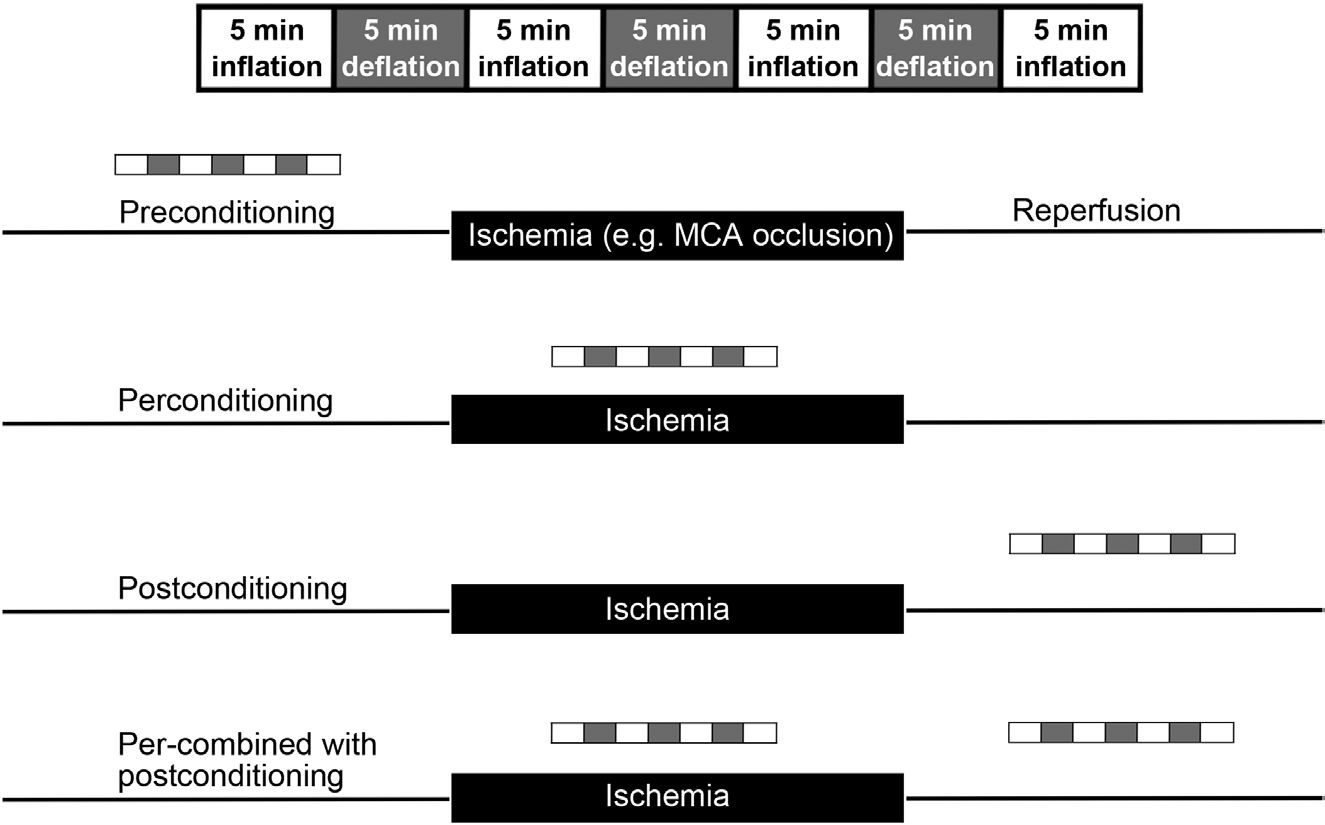
\includegraphics[width = \textwidth]{billeder/PrePerPostKonditionering.png}
	\caption{Oversigt over de forskellige former for RIC behandling. Kilde: \cite{RefWorks:3}}\label{fig:cycles}. 
\end{figure}

\subsection{Mekanismer}
Ligesom at der endnu ikke er evidence for at en bestemt tid pr cyklus og bestemt antal cyklusser, så hersker der også stor tvivl i hvilke mekanismer som er afgørende for at konditioneringen har effekt.  Dog er der eftervist en lang række mekanismer og endogene responser, som opstår når kroppen udsættes for konditionering. Ved behandling med RIC øges det cerebrale flow ved hjælp af en række mekanismer, bla. ved et forhøjet niveau af nitrit og microRNA-144. I iltfattige område omdannes nitrit til nitrit oxid og dette medfører dilation af blodkarrene. Nitrit har ydermere en effekt på mitokondrierne. Mitokondrierne producere energi til cellen og uden den dør cellen. Nitrit øger mitokondriernes tolerance over for iltmangel. MicroRNA-144 medvirker også til den gavnlige effekt af RIC ved at påvirke cirkulationen.
RIC har også vist at aktivere en række mekanismer i forbindelse med nervesystemet (Se figur \ref{fig:mechanism}. Under RIC er der en øget aktivitet af det autonome nervesystem, og især vagusnerven er aktiv. Blokeres responsen fra vagusnerven mindske effekt af RIC. Dette skyldes at vagusnerven indgår i et anti-inflammatoriske system, og øget aktivering af nerven reducerer inflammation ved fx. iskæmisk-reperfusionsskader. Studier har også vsit at RIC reducerer den inflammatoriske genekspression \cite{RefWorks:20}, \cite{RefWorks:3}. Ydermere  øger udskillelsen af endogene opioider muligvis aktiveringen og reguleringen af immunceller. Især den reducerede celledød ved behandling med RIC kan forbindes med sænket immunrespons. Hormonel påvirkning er også påvist i forbindelse med RIC. Den iskæmiske tilstande i kroppen har vist et øget udskillelse af fx. adenosine og bradykinin. Begge stoffer, bradykinin og adenosine har indvirkning på cirkulationen og blodflowet. Bradykinin dilaterer blodkarrene og sænker dermed trykket. Adenosine er flow regulerende, påvirker ATP produktionen og medfører øget signal transmission over cellemembranen \cite{RefWorks:3}.

\begin{figure}[H]
	\centering
	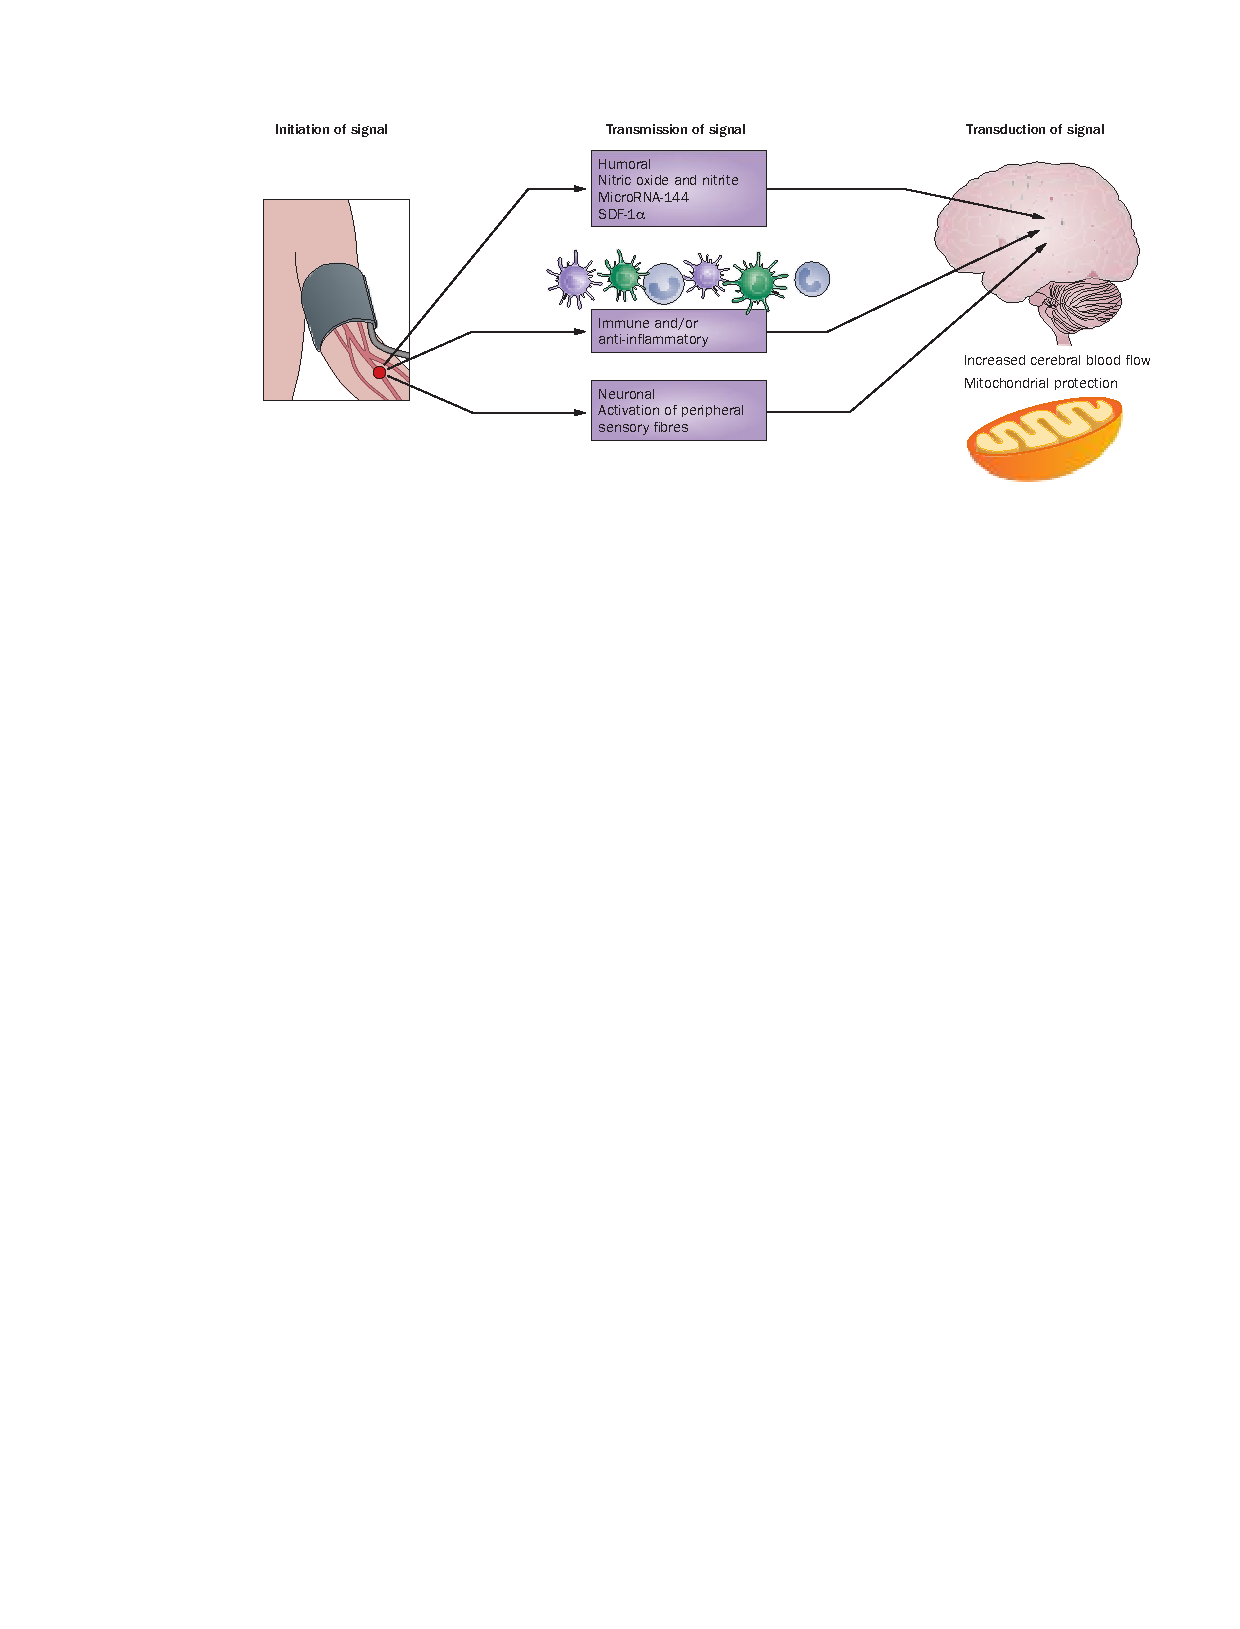
\includegraphics[width = 0.7\textwidth]{billeder/Konditioneringsmekanismer.png}
	\caption{Oversigt over mulige mekanismer der kan aktiverings under konditionering, kilde: \cite{RefWorks:3}} \label{fig:mechanism}
\end{figure}

\subsection{Studieprotokol}
Mange faktorer omkring RIC er endnu ukendt og især effekten af behandling mangler evidence. Et kommende studie for neurologisk afsnit på Aarhus Universitetshospital (AUH) ønsker at undersøge effekten af RIPerC og RIPpostC, for at forbedre den kliniske rutine til behandling af patienter med akute iskæmiske stroke. \fixme{Rerence til studieprotokol} Studiet skal foretages på patienter med akut iskæmiske stroke(AIS), som modtager trombolysebehandling. Patienterne udvælges tilfældig så nogle ikke vil modtage RIC. Studiet evaluerer patienter på en række kriterier, heriblandt størrelsen af infarktet efter trombolyse, RIPerC, RIpostC og det kliniske output, som bliver vurderet på \textit{modified Rankin Scale}. Der findes allerede studie, som har testet effekten af RIC på patienter med blodprop i hjerte og da disse ofte har et lavt blodtryk, findes der kun apparatet til okkludere armen ved 200mmHg. Da studiet undersøger patienter med AIS, som kan have blodtryk på over 200mmHg skal studiet bruge et modificeret blodtryksapparat, der kan håndterer systolisk blodtryk på over 200mmHg. Dette er nødvendigt for at sikre tilstrækkelig okklusion.

\section{Noninvasiv blodtryksmåling}\label{noninvasivBloodpressureMeasurement}
Noninvasiv blodtryksmåling, eller indirekte måling af det arterielle blodtryk er fællesbetegnelsen, for flere typer af tekniker, som alle estimerer blodtrykket i arteriet. Ofte associeres en blodtryksmåling af denne type, med den manuelle auditive detektion af puls, distal til en okkluderende manchet, som kan ses på figur \ref{fig:audiotoryBloodpressureMeasurement}. Denne manuelle auskulatoriske metode med kviksølvs sphygmomanometer anses stadig for at være guldstandarden inden for noninvasiv blodtryksmonitorering, \cite{RefWorks:24} .

\begin{figure}[H]
	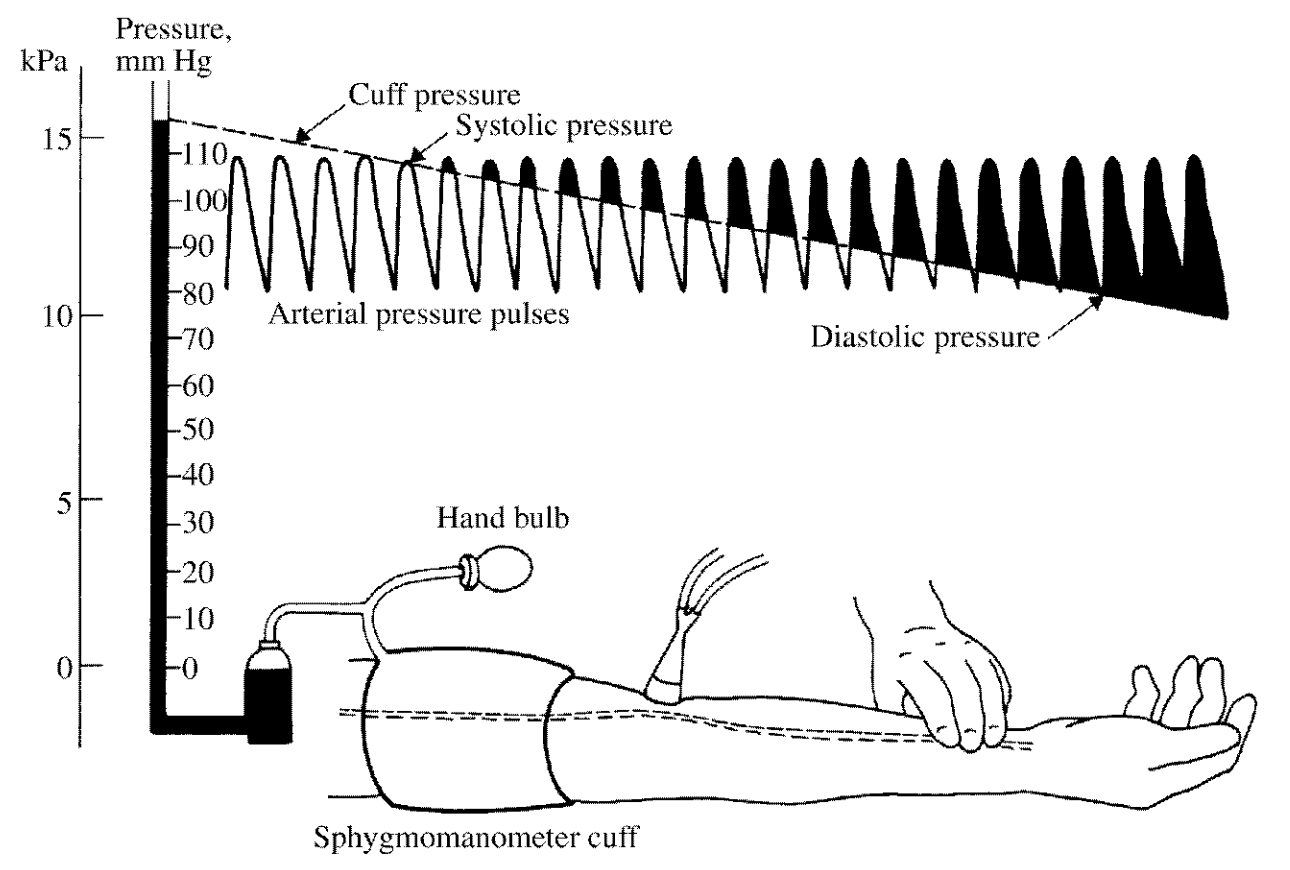
\includegraphics[width=0.9\textwidth]{billeder/TypicalIndirectBlood-pressureMeasurement.png}
	\caption{Typisk indirekte blodtryksmåling med sphygmomanometer, manchet ogstetoskop, kilde: \cite{RefWorks:27}, side 325}\label{fig:audiotoryBloodpressureMeasurement}
\end{figure}

Det automatiske blodtryks apparat som erstatter den manuelle auditive metode (automatiseret auskultatorisk apparat) anvender i alt sin simpelhed en mikrofon i stedet for stetoskopet. Ultralyd anvendes også i nogle blodtryksapparater som erstatning af stetoskoppet og bestemmer ved hjælp af doppler, hvornår arteriet er total okkluderet af manchetten. Ultralyd har særlige fordele, såsom at kunne bruges på spædbørn og hypotensive patienter, hvor lyden af blodflowvibrationerne i arteriet kan være svære at hører. Langt de fleste blodtryksmållere anvender dog i dag den oscillometriske metode, hvor selve manchetten selv agerer som interface til det pulserende arterie (se figur \ref{fig:OscillometriskMetode}), \cite{RefWorks:24} . Det ekspanderende arterie skubber til manchetten og skaber oscilloerende trykændringer i manchetten. På samme måde, som ved den auskultatoriske metode pumpes trykket i manchetten til over systolisk blodtryk, hvor arteriet er total okkluderet og manchetten udsættes på dette stadie ikke for pulsationer fra det underlæggene arterie. Luften i manchetten lukkes gradvist ud over tid. Når arterie trykket overstiger manchet trykket løber blodet ind i arteriet og skubber til arterievæggen. De små oscillotioner overføres til manchetten, hvilket resulterer i trykændringer (de største trykændringer i manchetten kan også observeres i sphygmomanometeret under en auskulatorisk måling). Oscillotionerne isoleres fra manchetrykket og kan ses på figur \ref{fig:OscillometriskMetode}. MAP ses hvor oscillotionerne er størst og det systoliske blodtryk ses hvor en pludseligt stigning i amplitude højden finder sted. Diastolen har ikke en klar overgang og er derfor bestemt ud fra algoritmer.\fixme{Webster side 328}

\begin{figure}[H]
	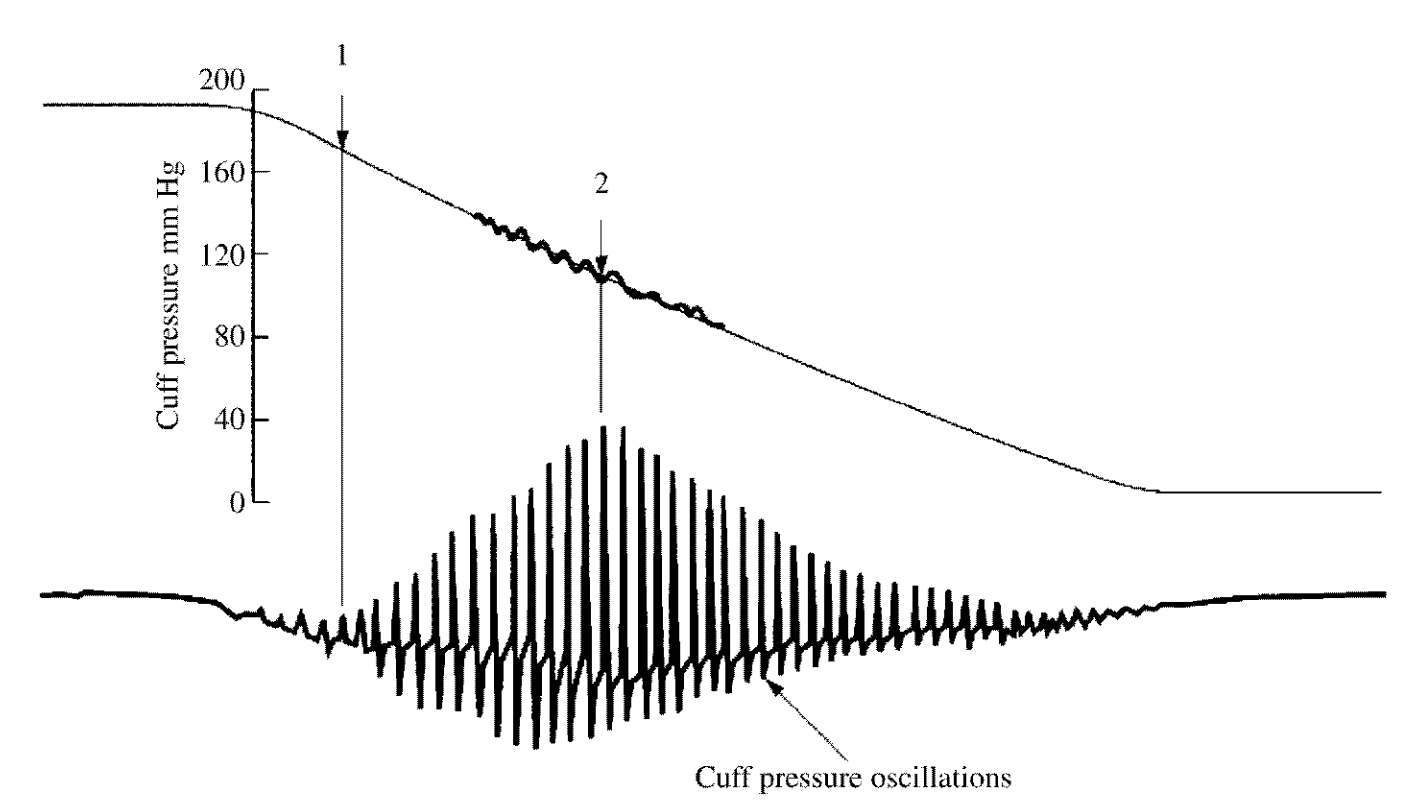
\includegraphics[width=0.9\textwidth]{billeder/OscillometriskMetode.png}
	\caption{Den oscillometriske metode. En kompressionsmanchet oppustes til et tryk over det systolisk blodtryk. Luften lukkes langsomt ud, hvorefter det systoliske tryk måles ved punkt 1 og MAP ved punkt 2. Det systoliske tryk ses ved den pluslige stigning i de oscillostionernes ampletuder og MAP er manchettrykket ved de største oscillotioner er til stede. Kilde: \cite{RefWorks:27}, side 329} \label{fig:OscillometriskMetode}
\end{figure}

\section{Okklusionstræning}
Okklusionstræning eller blood flow resistance (BFR) træning har i det senest år gennemgået mange undersøgelse og har vist en stor effekt i forbindelse med muskel hypertrofi og styrke. Ved normal styrketræning skal en utrænede person arbejde omkring 45-60\% af 1 repetition maks (RM) for at opnå hypertrofi og øget styrke, og hos en trænet person skal man ligge omkring 80-85\% af 1-RM. Ved okklusionstræning skal belastningen ligge væsentlig lavere, omkring 20-50\% af 1-RM, for at opnå samme eller større effekt. 
Okklusiontræning udfører ved at afklemme blodforsyningen til muskel, så manchetten sidder proximalt for musklen. Trykket der okkluderes ved varierer meget fra studierne. Imens musklen er okkluderet arbejder personen til udtrættelse. Dette gentager i et ønskede antal set. 
Pga. det lave belastning og det relativt korte træning periode og stadig store effekt, egner det træningsform sig ideal for person med ledskader, til genoptræningsforløb eller til person som har været sengeliggende længe, \fixme{Reference til The efficacy of blood flow restricted exercise: A systematic review and meta-analysis}










\chapter{Problemformulering}\label{title:problemformulering}
<<<<<<< HEAD
Som beskrevet i baggrundsafsnittet (Se afsnit \ref{chap:Baggrund}) ønsker en forsker gruppe ved Aarhus Universitetshospital(AUH) at undersøge effekten ved per og postkonditionering. Til dette formål bruges et modificeret blodtryksapparat, som kan indgå i forskningsprojekt til at foretage per og postkonditionering på forsøgspersonerne. Kunden har i samarbejde med Aarhus Universitet udarbejdet et bachelor projekt opslag med følgende punkter:
=======
Som beskrevet i baggrundsafsnittet (Se afsnit \ref{chap:Baggrund}) ønsker en forsker gruppe ved Aarhus Universitet Hospital at undersøge effekten ved per og postkonditionering. Til dette formål skal der bruges et modificeret blodtryksapparat, som kan indgå i forskningsprojekt til at foretage per og postkonditionering på forsøgspersonerne. Kunden har i samarbejde med Aarhus Universitet udarbejdet et bachelor projekt opslag med følgende punkter:
>>>>>>> origin/master
\begin{itemize}
	\item Samarbejde med en dansk producent af blodtryksappart
	\item Samarbejde med forsøgsansvarlige læger omkring produktkrav
	\item Designe et modificeret blodtryksapparat
	\item Samarbejde med produktionsvirksomhed i Kina omkring udvikling af prototype 
	\item Test af prototype udfra præspecificerede data
\end{itemize}

I samarbejde med projektvejleder Peter Johansen og projektudbyder Rolf Blauenfeldt har bachelorprojektet ændret karakter, fra at prototypen skulle fremstilling hos en kinesisk producent, til at bachelor gruppen selv fremstiller en \textit{proof of concept} prototype. Selvom bachelorgruppen selv udvikler prototypen ønskes det stadig fra kundens side at der bliver samarbejdet med den danske producent, for at sikre at prototypen ville ligge sig tæt op af deres blodtryksmålere.

For at produktet skal kunne bruges til konditioneringsbehandling skal det kunne måle et blodtryk, hvor efter der afklemmes i specificerede cyklusser. Afklemningstrykket skal være 25 mmHg over systolisk tryk for at sikre tilstrækkelig arteriel okklusion. De specificerede antal cyklusser fungerer, så forholdet mellem okklusion og reperfusion er en-til-en. 

Fra kundens side lyder endvidere et krav til konditioneringsprotokolen kan ændres, hvis forskningen viser bedre effekt ved en anden protokol. De ændringer der skal kunne foretages i protokollen er tiden en cyklus varer og antallet af cyklusser en konditioneringsbehandling skal have. 

Da patienten der skal modtage konditioneringsbehandling skal have armen afklemt i længerevarende perioder, er der fra kundens side stillet et krav omkring sikkerhedskontrol. Sikkerhedskontrollen stiller krav til at prototypen skal foretage et kredsløbstjek og vurdere om patienten kan risikere at tage skade af de iskæmiske tilstande, som den afklemte ekstremitet udsættes for under behandlingen.

<<<<<<< HEAD
Udover behovet for et apparat der kan udføre konditionering, er der efter foreslag fra vejleder Peter Johansen et ønske til prototypen skal kunne bruges til okklusionstræning. Som to separate funktioner skal prototype kunne skifte mellem konditioningsforløb og okklusionsforløb. Ved okklusionstræning er kravet at man holder et konstant tryk i manchetten på omkring 100mmHg. 
=======
Udover behovet for et apparat der kan udføre perkonditionering, er der efter foreslag fra vejleder Peter Johansen et ønske til at prototypen skal kunne bruges til okklusionstræning. Som en separat funktion skal prototype kunne skifte mellem konditioningsforløb og okklusionstræningsforløb. Ved okklusionstræning er kravet at trykket i manchetten holdes konstant på omkring 100mmHg. 
>>>>>>> origin/master


\chapter{Projektafgrænsninger}
Dette kapitel beskriver projektets afgrænsninger og hvilke arbejdsopgaver der blevet frasorteres i udviklingsfasen. Afgrænsninger kan både være til der er helt undladt i projektet, eller bestemte faktorer der har begrænset udvikling af vise dele i systemet. 

\section{Sikkerhedskontrol} \label{title:sikkerhedskontrol}
Fra projekts start i forprojektet lå der et ønske fra kunden siden omkring en sikkerhedskontrol ved konditioneringsbehandlingen. Fra kunden side bestod ønsket i at kontrollere kredsløbet på patienten, der modtog konditioneringsbehandling. Ønsket lød på at bruge et pulsoximeter som sikkerhedskontrol. Det færdige produkt skulle ved hjælp af et pulsoximeter tjekket patients saturation og puls og ud fra threshold værdier vurdere om patienten kunne tåle behandlingen. De tilfælde, der blev nævnt som kunne få sikkerhedskontrollen til at afbryde behandling, var patient med dårligt kredsløb, som ikke kunne nå at opfylde iltreserven i armen i reperfusionsfasen. Problematikken ved at bruge et pulsoximeter som sikkerhedskontrol ligger i teknikken bag pulsoximeteri. 

Pulsoximeteri måler variationer i det pulserende blod ved at detektere ændringerne i absorption af lys fra en to lyskilder med forskellige bølgelængder. Når væv belyses kan absorption grundlaget opdeles i fire dele (Se figur \ref{fig:opticTissue})
\begin{figure}[H]
	\centering
	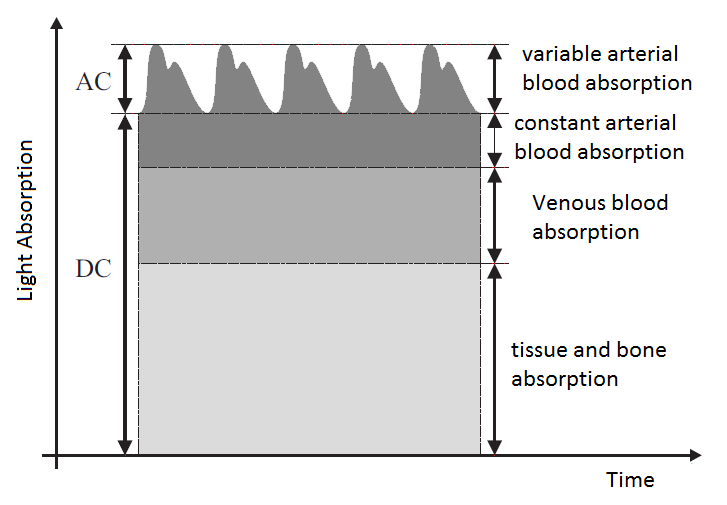
\includegraphics[width = 0.7\textwidth]{billeder/opticTissue.png}
	\caption{Oversigt over absorption af lys i væv}\label{fig:opticTissue}
\end{figure}

I pulsoximeteri filtreres alt DC væk, dvs absorption fra venøst blod, den konstante mængde af arterielt blod og alt andet væv og der kigges kun på signal fra det pulserende arterielle blod. For at måle saturationen udregnes forskellen på absorption ved \textit{pulstop} og \textit{pulsbund}. Disse absorption kan ved hjælp af de molar extinction koefficienter for hhv. oxyhæmoglobin og deoxyhæmoglobin og afstanden mellem lyskilde og modtager omregnes til relative koncentrations ændring i hhv. oxyhæmoglobin og deoxyhæmoglobin. Disse relative koncentration ændringer kan så omsættes til saturation via formlen \ref{eq:satequation}
\begin{equation}
	SaO_2 = \frac{\Delta[HbO_2]}{\Delta[HbO_2]+\Delta[HHb]}
	\label{eq:satequation}
\end{equation}

På grund af pulsoximeteri kun giver oplysninger omkring pulserende arteriel blod og at iltforsyningen af væv foregår via kapillærerne, mangler der information om kredsløbet i kapillærerne. På den måde giver pulsoximeteri en indikator for respirationen og for hvor iskemisk vævet er. Sikkerhedskontrollen skulle kontrollere om iltreserven i armen nået op på et tilstrækkeligt niveau efter hver afklemning, men pga det pulserende signal fra dette arterielle blod er meget små signaler, er et pulsoximeter udviklet til at detektere meget små signal. Derfor kan selv en person med dårlig kredsløb få målt en puls og saturation uden at vide om hans væv tager skade af konditioneringsbehandlingen. 

Denne problemstilling blev opdaget forholdsvis hurtigt i projektforløbet og kunden blev orienteret omkring problemstillingen. Det blev derfor bestemt at projektet skulle afgrænses i forbindelse med sikkerhedskontrollen. Der er gjort plads i udviklingsdokumentation til at implementering af en anden form for sikkerhedskontrol. For at få underbygget påstanden omkring pulsoximeteri og sikkerhedskontrol, har projektgruppen været i kontakt med Troels Johansen fra lungemedicinsk afsnit på AUH (Se afsnit \ref{title:samarbejdspartnere} omkring samarbejdspartnere og mødereferater \fixme{Reference til mødereferat med Troels Johansen}). Troels kunne kun bekræfte påstanden omkring at pulsoximeteri som være ugyldig til sikkerhedskontrol, og så istedet muligheder i NIRS(Se afsnit \ref{title:nirs} i perspektivering) eller at bruge pulsoximeteri som kontrol af om afklemningen var tilstrækkeligt. 

\section{MR kompatibilitet}
I forbindelse med forprojektet var et ønskescenarie fra kunden side at apparatet der skulle udviklings til at udfører konditionering skulle kunne gå i en MR-scanner. Dette var et ønske fordi perkonditionering, hvis det køres i fx 4 cyklusser af 5 minutter, vil tage længere til at gennemfører, end den tid det tager at kører til hospitalet. Proceduren for patient der mistænkes for have apopleksi er at få dem i MR scanneren så hurtigt så muligt, og derfor kan man i nogle tilfælde være nød til at afbryde konditioneringsbehandlingen og der kan stilles spørgsmålstegn ved den gavnlige effekt. Det blev meget hurtigt bestemt af projektet måtte afgrænse sig fra at lave apparatet MR kompatibel, da dette ville stille alt for høje krav til produktets komponenter.

\section{Signal behandling}

\section{Seagull samarbejde}
I begyndelse af projektet blev der igennem kunden etableret et sammen arbejdet med en dansk virksomhed, som skulle fungere som talerør til en kinesisk blodtryksapparat producent (Se afsnit \ref{title:samarbejdspartnere} omkring samarbejdspartnere). Tanken bag samarbejdet var et den kinesiske virksomhed skulle kunne bestå med komponenter og teknisks sparringen. Grunden til den danske virksomhed var med som mellemmand var et ønske fra deres side, da den kinesiske virksomhed var deres kontakt. Et andet argument for at det skulle være sammen arbejde med virksomheder var et ønskede fra kunden side omkring produktet skulle lige sig tæt opad Seagulls apparatet. 

Men efter flere forgæves forsøg for at kommunikere og få information ud af den kinesisk virksomhed blevet det opgivet at produktet skulle ligge sig op af deres apparater. Det forgæves samarbejde betød også at arbejdet med en blodtryksalgoritme måtte foretages på egen hånd af projektgruppen selv. 

\section{Prototypen}
\chapter{Systembeskrivelse}
Det giver kapitel indeholder en gennemgang af den udviklede prototype, kaldet \textit{Konditioneringsapparatet}. Kapitlet har til formål at give læseren en forståelse af \textit{Konditioneringsapparatet} og for at sikre forståelsen af kommende kapitler. Det afsnit skal derfor ikke ses som værende en opsummering af projektets resultater, her henvises til kapitel \ref{title:resultater}.

\textit{Konditioneringsapparatet} er en prototype og et \textit{proof of concept} apparat der kan udføre konditioneringsbehandling og okklusionstræning. På figur \ref{fig:systemTegning} ses en oversigt over systemet. Overordnet set består prototypen af én strømforsyning, ét pneumatisk system, én styringsenhed, én timer og ét display. Det pneumatiske system kan yderlige opdeles i 4 dele; ventil, motor, blodtryksmanchet og tryksensor. Styringsenheden består af en microkontroller og et motorshield. 

\begin{figure}[H]
	\centering
	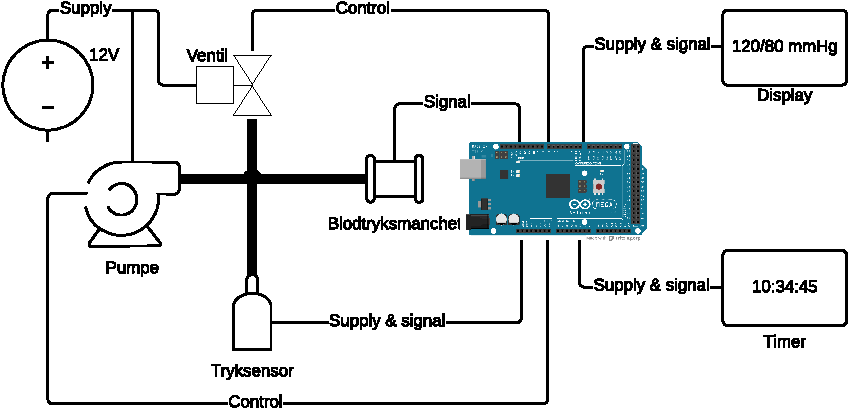
\includegraphics[width = \textwidth]{billeder/systemDrawing-crop.pdf}
	\caption{Oversigt over \textit{Konditioneringsapparatet}} \label{fig:systemTegning}
\end{figure}

Prototypen kan som beskrevet udføre konditioneringsbehandling og okklusionstræning. Begge funktioner kræver at manchetten monteres på enten armen eller benet. Ved konditioneringsbehandling måles blodtrykket og der afklemmes ved et tryk svarende til 25mmHg højere end det målte systoliske tryk. Dernæst udføres konditioneringsbehandling. Systemet logger information omkring konditioneringsbehandling. Okklusionstræning udføres ved at pumpe manchettrykket op til 100 mmHg og holde det tryk indtil brugeren stopper forløbet. 

Endvidere kan \textit{konditioneringsapparatet} konfigureres så der kan køres varierende antal cyklusser og tid pr cyklus.


\section{Brugergrænseflade}
\textit{Konditioneringsapparatets} brugergrænseflade består af 2 knapper og en skærm. Desuden findes en \textit{modeswitch} på prototypen, en \textit{modeswitch} er en knap med 3 stadier, som styre hvilket program prototypen skal udføre.  

\section{Data logging}
Systemet kan gemme information omkring konditioneringsbehandling. Disse gemmes på et SD kort og det gøres for at sikre at dokumentation af de udførte behandlinger.
\chapter{Metoder}
Metode kapitlet beskriver projektets arbejdsmetoder, hvilke metoder der brugt og hvordan de er blevet brugt. Metodeafsnittet vil især beskrive projektstyringsforløb og udviklingsmetoderne. 

\section{Projektstyring} \label{title:projektstyring}
Til overordnet projektstyring er der gjort brug af den \textit{Struktureret Agile Metode}, forkortet SAM. (Se hjemmeside \fixme{Reference til http://www.agilemanifesto.org/iso/dk/}). Metoden karakteriseres ved at inddele projektet i følgende faser: krav, design, implementering og test. Metoden passede godt på projektet i flere omstændigheder. SAM er oplagt til projektgrupper i størrelsen 2-3 personer og projekter der varer 3-9 måneder. Metoden er også særlig anvendelig til projektet da inddragelse af kunden fylder en stor del i arbejdet. 
Især i arbejde med forprojektet og opstartsfasen på projektet blev der afholdt mange møder for at fastlægge projektets rammer og kravene til produktet. I SAM metoden adskiller man møder i forskellige kategorier og de tre kategori er som følger: \textit{introduktionsmøde, planlægningsmøde og kontraktmøde}. Samarbejdet med kunde Rolf Blauenfeldt kan meget vel inddeles i tre forskellige møde kategorier. I forprojektet afholdte projektgruppen \textit{introduktionsmøde} med kunden for at forventningsafstemme. Da det var på plads og projektgruppen havde besluttet at kundens problemstilling var en opgave som gruppen kunne løse, blev der afholdt flere \textit{planlægningsmøder} for at finde og udspecificere de  krav som kunden havde til produktet. Disse møder er afholdt over flere omgange, da der undervejs i projekt er opstået situationer, som ikke var blevet fastlagte. Men efter der var afholdt tilstrækkeligt \textit{planlægningsmøder} igangsatte projektgruppen første fase af SAM metoden og der blev udarbejdet en kravspecifikation(Se afsnit \ref{title:kravspecifikation}). SAM faserne er iterative processer, derfor blev der undervejs i forløbet  foretaget ændringer og justeringer i kravspecifikationen. Kort efterfulgt af kravspecifikation er der udarbejdet en accepttest (Se afsnit \ref{title:accepttest}), som blev udfyldt da udviklingen af prototypen var færdig. Inden arbejdet med prototypen begyndte, blev der udarbejdet et system design (Se afsnit \ref{title:systemdesign}), for at fastlægge hvordan systemet skulle struktureres. Da system strukturen var fastlagt begyndt implementeringsfasen og slutter med at gennemføre accepttesten. For uddybende information se afsnit \ref{title:udviklingMetode} omkring udviklingsdokumentationen.

\subsection{Scrum/Pivotaltracker} \label{title:scrum}
Til arbejdsfordeling og planlægning af arbejdsopgaver er projektet udarbejdet ved hjælp af scrum. Der er ikke brugt scrum i direkte forstand. Men hver uge er blevet set som et sprint, hvor der hver mandag er udarbejdet en sprint backlog som skulle udføres i ugens løb. Emnerne til sprint backlogen er bla. taget fra tidsplanen som kan ses som en overordnet projekt backlog. Sidst på ugen er der afholdt møde, hvor der opsamles på ugens arbejdet og hvilke opgaver i sprint backloggen der er blevet løst. Opgaver, der ikke blev løst, er automatisk blevet videreført til næste uges backlog. Hver mandag når der oprettes et sprint backlog er disse opgaver blevet oprettet i projektstyringsværktøjet \textit{pivotaltracker}. ( se hjemmeside \fixme{https://www.pivotaltracker.com/}). 

\subsection{Samarbejdsaftale}
For at sikre interne forventninger til projektarbejde i gruppen, har gruppens medlemmer lavet og underskrevet en samarbejdsaftale i begyndelse af projektet. Aftalen kan læses i \ref{title:samarbejdsaftaleIntern}.

I forbindelse med samarbejdet med reviewgruppen, er der også blevet udarbejdet og underskrevet en samarbejdsaftale, for at sikre ens forventning til reviewmøderne. Aftalen kan læses i \ref{title:samarbejdsaftaleReview}.

\subsection{Samarbejdspartnere} \label{title:samarbejdspartnere}
Dette afsnit beskriver projektgruppens samarbejdspartnere igennem projektet. 

\textbf{Kunden og projektudbyder:} Rolf Ankerlund Blauenfeldt er læge ved neurologisk afsnit på Aarhus Universitet (AUH). Samarbejdet med Rolf har primært bestået i specificering af krav til udvikling af \textit{Konditioneringsapparatet} samt faglig ekspert for remote ischemic conditioning (RIC). Desuden er det kunden som godkender accepttesten.

\textbf{Vejleder:} Projektvejleder Peter Johansen, har været som faglig vejleder i gennem hele projektet og igennem vejledermøder Peter bistået med faglig kritik løbende. 

\textbf{Reviewgruppe:} Igennem projektet er der samarbejdet med en anden projektgruppe, hhv. Anders Esager og Anders Toft. Denne gruppe har fungeret som opponent/review gruppe, og hver gang en milepæl var nået, fx accepttest, har grupperne reviewet hinandens opgaver, hvorefter et møde er blevet afholdet og rettelserne er blevet gennemgået.  

\textbf{Firma:} Virksomheden Seagul forhandler blodtryksapparater og har i projektets opstart fungeret som kontaktperson til en kinesisks udviklingsvirksomhed. Samarbejdet blev oprettet for at projektgruppen kunne modtage teknisk sparring i specifikations- og udviklingsfasen. 

\textbf{Advokat:} I forbindelse med tavshedspligt (Se afsnit \ref{title:tavshedspligt}) har projektgruppen samarbejdet med juridisk rådgiver Maibrit Lerche Hendriksen fra Aarhus Universitet. Pga. projektgruppen ønskede samarbejde med en reviewgruppe, kunne samarbejdet ikke begynde før reviewgruppen også blev underlagt tavshedspligt.

\subsubsection{Medikoteknisk afd. AUH}
Til udvikling og kalibrering af \textit{Konditioneringsapparatet} har projektgruppen samarbejdet med medikotekniske ingeniører  Sara Rose Newell og Steven Brantlov fra Region Midtjylland. Disse har kunne bistå med en blodtrykssimulator, samt teknisk forståelse af blodtryksmåling. Samarbejdet har bestået i mail korrespondance, samt to møder på medikoteknisk afsnit på AUH, hvor projektgruppen har testet og kalibreret \textit{Konditioneringsapparatet} på blodtrykssimulatoren. 

\subsubsection{Lungemedicinsk afsnit og Troels Johansen}
I forbindelse med udvikling af sikkerhedskontrol til konditioneringsapparatet(Se afsnit \ref{title:sikkerhedskontrol} omkring projektafgrænsninger) har projektgruppen samarbejdet med Troels Johansen, PhD studerende ved lungemedicinsk afdelingen på AUH. Samarbejdet opstod pga. gruppen manglede ekspertviden omkring pulsoximeteri og afklemning.

\subsubsection{Institut for idræt og Kristian Vissing} 
Efter okklusionstræning blev en del prototypens funktionalitet, havde projektgruppen behov for mere indsigt omkring træningsformen. Her blev etableret et samarbejde med Kristian Vissing, lektor og forsker ved Institut for Idræt, Aarhus Universitet.  

\subsection{Ugeplan og logbog}
Som del af projektstyring, udviklingsproces, samt dagbog, er der på ugentlig basis udarbejdet en plan. Hver uge starter med en ugeplan og afsluttes med en logbog. Ugeplanen indholder de opgaver projektgruppen skal løse i ugens løb og logbogen er en opsamling på ugens arbejde. For uden at fungere som sprint backlog i scrum (Se afsnit \ref{title:scrum}) har logbogen også fungeret som en slags dagbog, hvor projekts forløb konstant er blevet beskrevet. Logbogen har også været særlig anvendeligt forbindelse med rapport skrivning. 

\subsection{Vejldermøde}
Fra projektets opstart blev der aftalt et vejledermøde i alle ulige uger under projektforløbet. Disse møder er blevet brugt til at sikre at projektarbejdet hele tiden var på rette spor, samt faglig vejledning til projektarbejdet. Desuden er vejledermøderne brugt til at få konstruktiv feedback på færdige dokumenter undervejs i forløbet. 

\subsection{Tidsplan}
I forbindelse med forprojektet blev der udarbejdet en tidsplan i gantt chart format (se afsnit \ref{title:tidsplan}). Et gantt chart illutreret start og slut dato for hvert af projektet delelementer. Hver række i tidsplanen udgør et delelement, fx. kravspecifikation og accepttesten og hver kolonne udgør én uge. Tidsplanen er løbende blevet opdateret efterhånden som projekt har nået delelementerne. 

\subsection{Tavshedspligt} \label{title:tavshedspligt}
Pga. af patentundersøgelse har hele projekt været underlagt tavshedspligt og underskrevet tavshedserklæringer med både universitet og neurologisk afsnit. Tavshedspligten har bla. forsinket nogle processer da alle parter skulle have underskrevet en tavshedserklæring inden. I andre tilfælde hvor et samarbejde har været kortvarig eller der ikke har været tid til at underskrive tavshedserklæring, har projektgruppen måtte undlade detaljer ved kommunikation med disse samarbejdspartnere. Dette har i nogle tilfælde betydet at hjælpen fra evt. eksperter har været begrænset af manglende forståelse for projektet.  Derfor har den igangværende patentundersøgelse været et begrænsning for projektarbejdet i flere omfang. \fixme{Reference til tavshedserklæring}
Tavshedspligten har også betydet at der skulle tages bestemte hensyn i forbindelse med versionsstyring. Ved brug af git (Se afsnit \ref{title:versionsstyring} omkring versionsstyring) som versionsstyrings værktøj, har gruppen skulle betale for at få et private repository. Dette er normal gratis, men så er ens repository offentligt tilgængeligt. 


\section{Versionsstyring} \label{title:versionsstyring}
For at sikre korrekt og brugervenlig versionsstyring af hele projektets versionsstyring blevet håndteret med git \fixme{Reference til git hjemmeside https://github.com/}. Git er versionsstyring primært udviklet til software. Styringen af versionshistorik fungere ved at der oprettes et respository, som ligger på en ekstern server. Hver gang der ønskes at arbejde på filerne i det oprettede repository, skal der synkroniseres, så den seneste version er tilgængelig. Foretages en ændring i en fil der køres versionshistorik på, skal denne \textit{committes} til ens repository. Alle ændringer der tilføjes, skal beskrives, for at sikre sporbarhed. Resten af versionsstyring foregår automatisk i git, og her gemmes automatisk versionsnummer og dato for ændring. Desuden gør git det også nemt at gå tilbage i versionshistorikken og finde tidligere versioner. 
Selvom prototypen \textit{Konditioneringsapparatet} ikke skal medicinsk godkendes, var det en grund til at vælge et detaljeret versionsstyrings system. Hvis et apparat skal medicinsk godkendelse stilles der store krav til dokumentationen, heriblandt versionsstyring, som indgår i kvalitetssikringen af produktet (Se afsnit \ref{title:medGodkendelse} ). 
Til grafisk interface findes en række programmer som gør git og versionsstyring mere brugervenligt, og her har det især været brugbart at kunne se forrige ændringer og tilføjelse. Dette har lettet projektarbejdet og mindsket uoverensstemmelser med hvilket dokument der er af seneste version. 

Udover git er dropbox brugt til at dele projektfiler, der ikke har behov for versionsstyring. Dette har fx. været videnskabelige artikler, datablade mm. 

\section{Udviklingsværktøjer}
\textbf{Eclipse:} er blevet brugt til software udvikling af \textit{Konditioneringsapparatet}. For at kunne simplificere kommunikation mellem eclipse og arduino boardet, er der blevet brugt et arduino plugin i eclipse. På den måde kan funktionaliteterne fra Arduino IDE bruges, samtidig med at eclipse funktionaliteter, som \textit{auto complete}, fejlhåndtering og projektstruktur også var tilstedet. 

\textbf{Arduino IDE:} er den oprindelig udviklingsplatform til arduino, men pga af manglende funktionalitet, er dette kun blevet brugt til simple enhedstests og små scripts. 

\textbf{Matlab:} Til databehandling og visualisering af signaler fra \textit{Konditioneringsapparatet}. Værktøjet er blevet brugt til at plotte tryk kurver fra tryksensoren, samt oscillationerne målt fra manchetten. Dette har været en stor hjælp for signal forståelse og i forbindelse med kalibrering af blodtryksmåleren. 

\textbf{Fritzing:} er blevet brugt til udarbejdning af fumlebræt tegning og schematics over hardware udvikling. Grundet prototype udviklingen har meget af arbejdet foregået på fumlebræt, og for at kunne dokumentere og "gemme" en opsætning på fumlebrættet har \textit{fritzing} været stor hjælp til bla. fejlhåndtering. \textit{Fritzing} er et open source program som er udviklet til dokumentation af prototyper. Da programmet er open source har processen med at finde nye komponenter været simpel. 

\textbf{Gimp:} Billede redigerings program som er blevet brugt til redigering og udarbejdelse af illustrationer. Især i forbindelse med figurer og illustrationer til latex har gimp været anvendeligt. 

\textbf{Maple:} Til filter udregning i forbindelse med design af analoge og digitale filtre er der blevet brugt Maple version 2015. Maple er kommercielt computer algebra system. 

\textbf{Modelio:} Alt udvikling af sysML og UML er foregået i Modelio. Modelio adskiller sig fra andre sysML værktøjer, da det ikke er et tegne program, men et programmeringssprog og IDE. Dette betyder at udviklingen af sysML har været begrænset af sproget, men det betyder også at det har været nemmere at overholde sysML standarden. 

\textbf{TexStudio:} Alt dokumentation er blevet udarbejdet i TexStudio. Dette er valgt for at få fuld kontrol over layoutet i dokumentationen og rapporten. LaTeX og TeXStudio gør også arbejdet med større projekter mere simpel, ved opdeling af dokumentationen i små underdokumenter.


\section{Udviklingsproces} \label{title:udviklingMetode}
Efter den struktureret agil metodes(SAM) fire faser: krav, design, implementering og test (se afsnit \ref{title:projektstyring}) er udviklingsprocessen foregået i denne rækkefølge. Disse fire faser vil blive beskrevet nedenfor.

	\subsection{Kravspecifikation} \label{title:kravspecifikation}
	Kravspecifikation er et dokument der beskriver de krav som produktet skal kunne. Der skelnes mellem funktionelle og ikke funktionelle krav. De funktionelle krav beskriver de essentielle krav for at produktet kan leve op til kundens behov. Et eksempel på et funktionelt krav er at apparatet skal kunne afklemme med tryk på 25 mmHg over det systoliske blodtryk. I kravspecifikation er de funktionelle krav beskrevet via \textit{fully dressed use cases}. En use case beskriver brugen med produktet i scenarier og ved hjælp af disse scenarier beskrives produktets funktionalitet. En \textit{fully dressed use case} indeholder, ud over en beskrivelse af hoved scenariet, også beskrivelse af hvilke aktører der er involveret i scenariet, samt før og efter betingelse for scenariet. I nogle scenarier kan det også være nødvendigt at beskrive undtagelser for forløbet, hvis disse ikke er for trivielle. Aktørerne der indgår i \textit{fully dressed use cases} er beskrevet med en aktørbeskrivelse i kravspecifikation. Her beskrives aktør rollen, og om han er primær eller sekundær. En primær aktør interagerer aktivt med produktet i use casen og er nødvendig for at scenariet lykkes. En sekundær aktør er passivt involveret med use casen og dette kan for eksempel være en patient der skal modtage behandling med et apparat. For at give læseren et overblik over sammenhængen mellem aktører og use cases, indeholder kravspecifikation et overordnet use case diagram, hvor alle scenerier er listet og aktørernes rolle er beskrevet med pile forbundet med use cases. 
	
	De ikke-funktionelle krav, er som navnet antyder, krav der ikke er nødvendige for produktets funktionalitet. Ikke-funktionelle krav er essentielle for brugervenligheden, sikkerheden og muligheden for at vedligeholde produktet. Ved specifikations af de ikke-funktionelle krav, indskærpes rammerne for udviklingen af produktet. Et eksempel på et funktionelt krav er at produktet skal kunne gemme information omkring konditioneringsbehandlingen på et SD kort. Her kan stilles et ikke-funktionelt krav, der specificeret datastrukturen på SD kortet og hvilken type SD produktet skal kunne håndtere. Det sikre brugervenlighed og sikkerhed, fordi brugeren ved hvordan data gemmes og hvilke SD kort der kan bruges i produktet. Herved imødekommes eventuelle data tab ved forkerte SD kort. For at fastlægge rammerne for udseende af prototypen, indeholder kravspecifikationen også illustrationer af bruger interfacet. 
	
	\subsection{Accepttest} \label{title:accepttest}
	Accepttest er en metode og en del af udviklingsprocessen, som er udarbejdet for at produktet kan leve op til kravspecifikation. Accepttesten er essentielt for produktudviklingen, for den udføres og godkendes i samarbejdet med kunden. Når accepttesten er gennemført er det kundens endegyldige godkendelse af produktet. 
	Dokumentet er struktureret med en tabel for hver use case, denne tabel indeholder punkterne fra hoved scenariet og hvert punkt indeholder en beskrivelse, en test metode, et forventet resultat og til sidste et felt hvor testen kan godkendes. Det samme struktur gælder for de ikke funktionelle krav. Hver test skal godkendes med underskrift af kunden.
	
	\subsection{System design} \label{title:systemdesign}
	Dette trin i udviklingsprocessen vedrører designet af \textit{Konditioneringsapparatet}. For at sikre overensstemmelse inden udviklingsprocessen blev igangsat, blev systemets design og arkitektur beskrevet. System designet indeholder først en beskrivelse af alle systemets underdele. Her beskrivelses hvilke dele der skal indgå i systemet for at det lever op til designet.
	For at sikre at alle områder i systemet designet blev belyst er der her gjort brug af metoden \textit{4 plus 1 modellen} på figur \ref{fig:4plus1model}. Modellen er oprindelig kun beregnet til software men i dette projekt er den tilpasset og bruges på systemet som helhed. 
	
	\begin{figure}[H]
		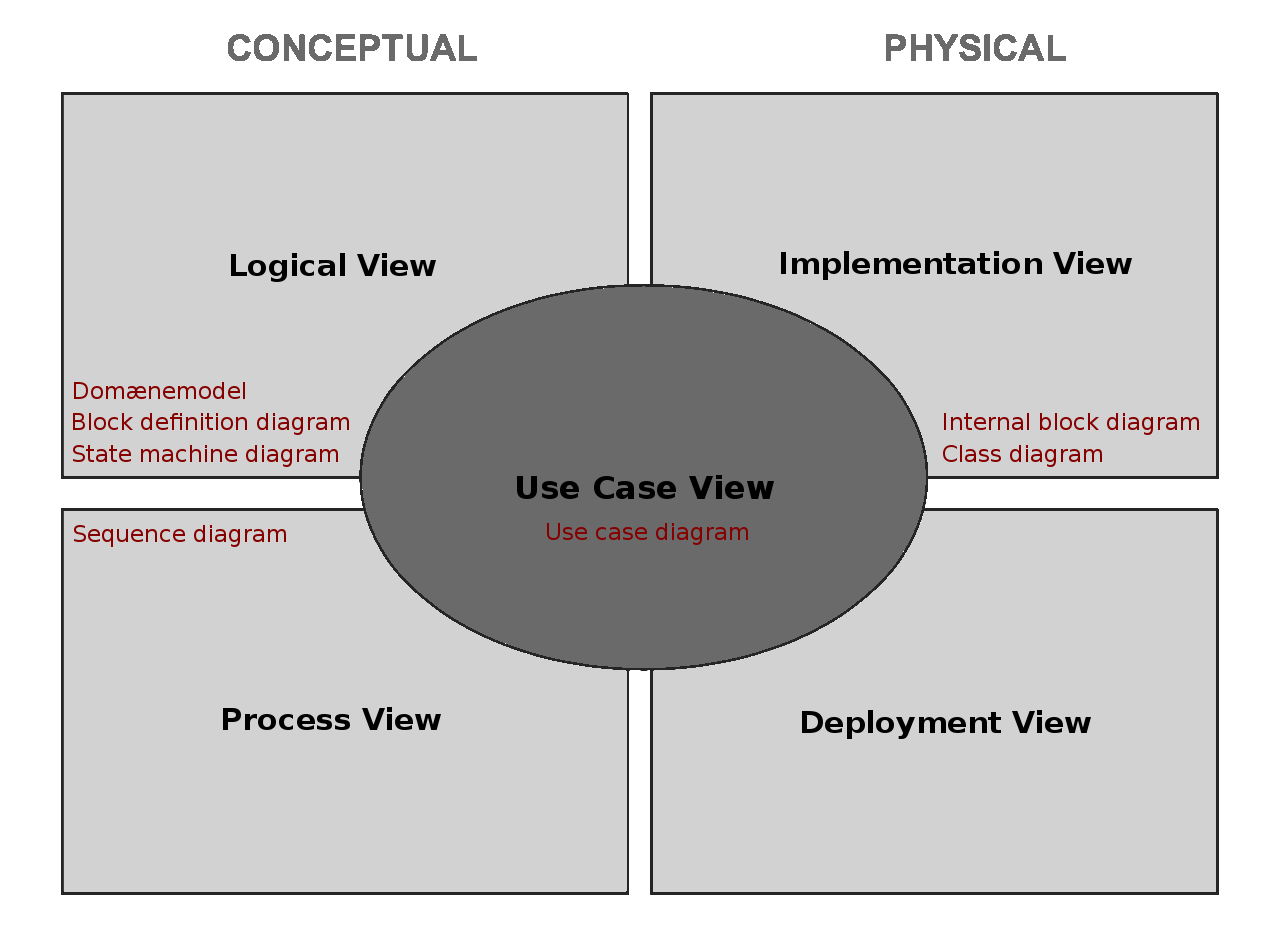
\includegraphics[width = \textwidth]{billeder/4plus1model.png}
		\caption{Tilpasset 4 + 1 model. Den røde tekst er de diagramtyper fra UML, som hører til de 5 inddelinger og er anvendt i dette projekt.}\label{4plus1model}
	\end{figure}
	
	4+1 modellen ser produktet fra fire forskellige synsvinkler og sikre at alle partners interesser er belyst. De fire synsvinker er som følger: 
	\\ \textit{Use case view}: Beskriver systemmet med aktører og de forskellige senarier de interagerer i. Dette er beskrevet i kravspecifikationen se (\fixme{ref: kravspec}).\\
	\textit{Logical view}: Denne synsvinkel beskriver systemets funktionalitet via centrale elementer, mekanismer og stadier. Synsvinklen er generelt mere abstrakt end de andre 3. \\
	\textit{Process view}: Beskæftiger sig med de dynamiske aspekter af systemet, forklaring system processer, hvordan de kommunikerer og fokuserer på systemets opførsel i drift. \\
	\textit{Implementation view}: Denne vinkel involverer udviklerens perspektiv og beskæftiger sig med hvordan software implementeres. \\
	\textit{Deployment view:} Beskriver systemet fra en fysisk synsvinkel, blandt andet hvordan eksekveringen af softwares skal foregå på apparatet og hvordan systemets fysisk setup skal ser ud. \\
	\textit{NB: Beskrivelse af de fire synsvinkler er udklip fra system design dokumentet.} \fixme{Indsæt reference til system design}
	
	I system design dokumentet er der også gjort stor brug af sysML diagram sproget. Sproget er universel blandt ingeniører og letter forståelsen af systemet. I \textit{Logical view} er der udarbejdet state machine diagrammer, som bruges til at beskrive stadierne som produktet kan befinde sig i, samt hvordan der skiftes mellem disse stadier. I \textit{process view} fokuseres der på hvordan systemet dele interagerer med hinanden. Til at beskrive denne kommunikation bruges sekvens diagrammer. Der er udarbejdet et sekvens diagram for hver use case. Sekvensdiagrammer beskriver hvordan scenarieret fra use case udføres i mellem systemets dele, samt hvilken information der videregives mellem underdelene. 
	
	\subsection{Implemetering} \label{title:implementering}
	Implementeringen af produktets funktionalitet er beskrevet i implementeringsdokumentet. Dette dokument bruges til at beskrive hvordan systemets enkelte software og hardware dele er implementeret og hvordan disse underdele har opnået deres ønskede funktionalitet. Dokumentet har også til formål at fungere som et opslagsværk, så ønsker læseren forståelse for en specifik software eller hardware del, står det i implementeringsdokumentet. Derfor skal implementeringsdokumentet også ses som en \textit{opskrift} på hvordan produktet er fremstillet. Dokumentet indeholder især erfaringer omkring arbejdet med systemets dele og hvordan de væsentlige dele er blevet enhedstestet. 

\subsection{V-model}
Den struktureret agile metode (SAM) indeholder samme faser som V modellen, men beskriver ikke på samme den iterative del af processen. V-modellen beskriver den iterative proces (Se figur \ref{fig:vmodel}). Modellen foreskriver at man starter med kravspecifikation og bevæger sig ned mod implementering hvorefter man i projektet arbejder op i mod accepttesten. Pilene i mellem beskriver at arbejdsprocessen er iterativ og fx de nederste 3 kasser; detaljeret design, implementering og unit test er den iterative proces meget brugbar. Når der opdages en fejl i implementering ændres designet og der gennemføres en ny enhedstest.  
\begin{figure}[H]
	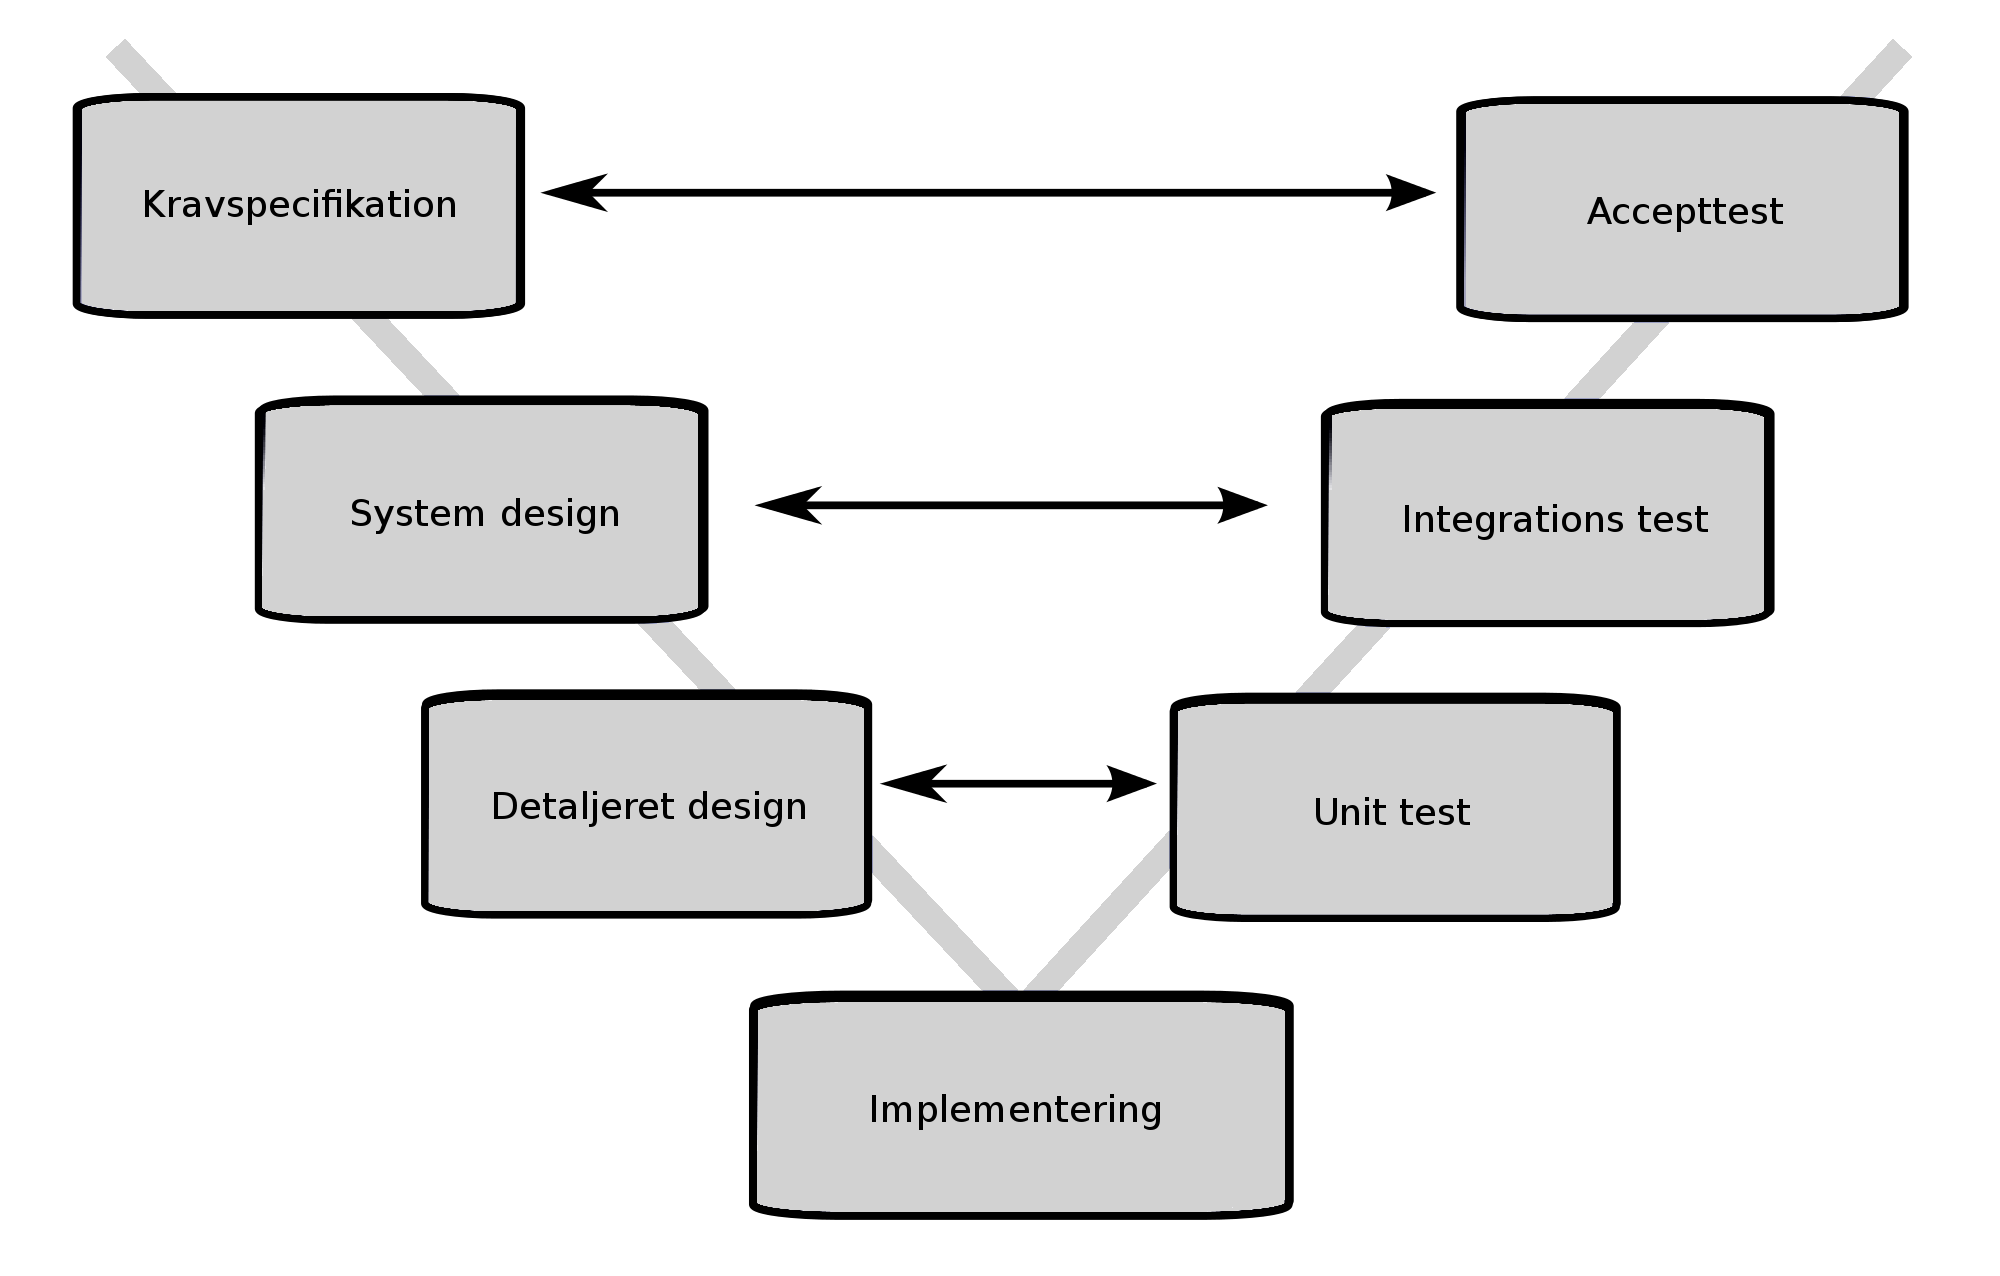
\includegraphics[width = \textwidth]{billeder/Vmodel.png}
	\caption{V-modellen}\label{fig:vmodel}
\end{figure}

\subsection{Review}
Review gruppen er beskrevet under afsnittet \ref{title:samarbejdspartnere}. Men review har også været en metode i udviklingsprocessen, i sammenfald med tidsplanen har reviewmøderne fungerede som deadline til hvornår bestemt mål skulle nåes i udviklingsprocessen. 

\subsection{3-lag modellen}
Denne metode bruges til at skabe struktur i \textit{Konditioneringsapparatets} software. 3-lags modellen sikre at der høj samhørighed og lav kobling mellem de tre lag. Inddelingen af konditioneringsapparatets software kan se system designet \fixme{Ref til system design} for mere information. 
\begin{figure}[H]
	\centering
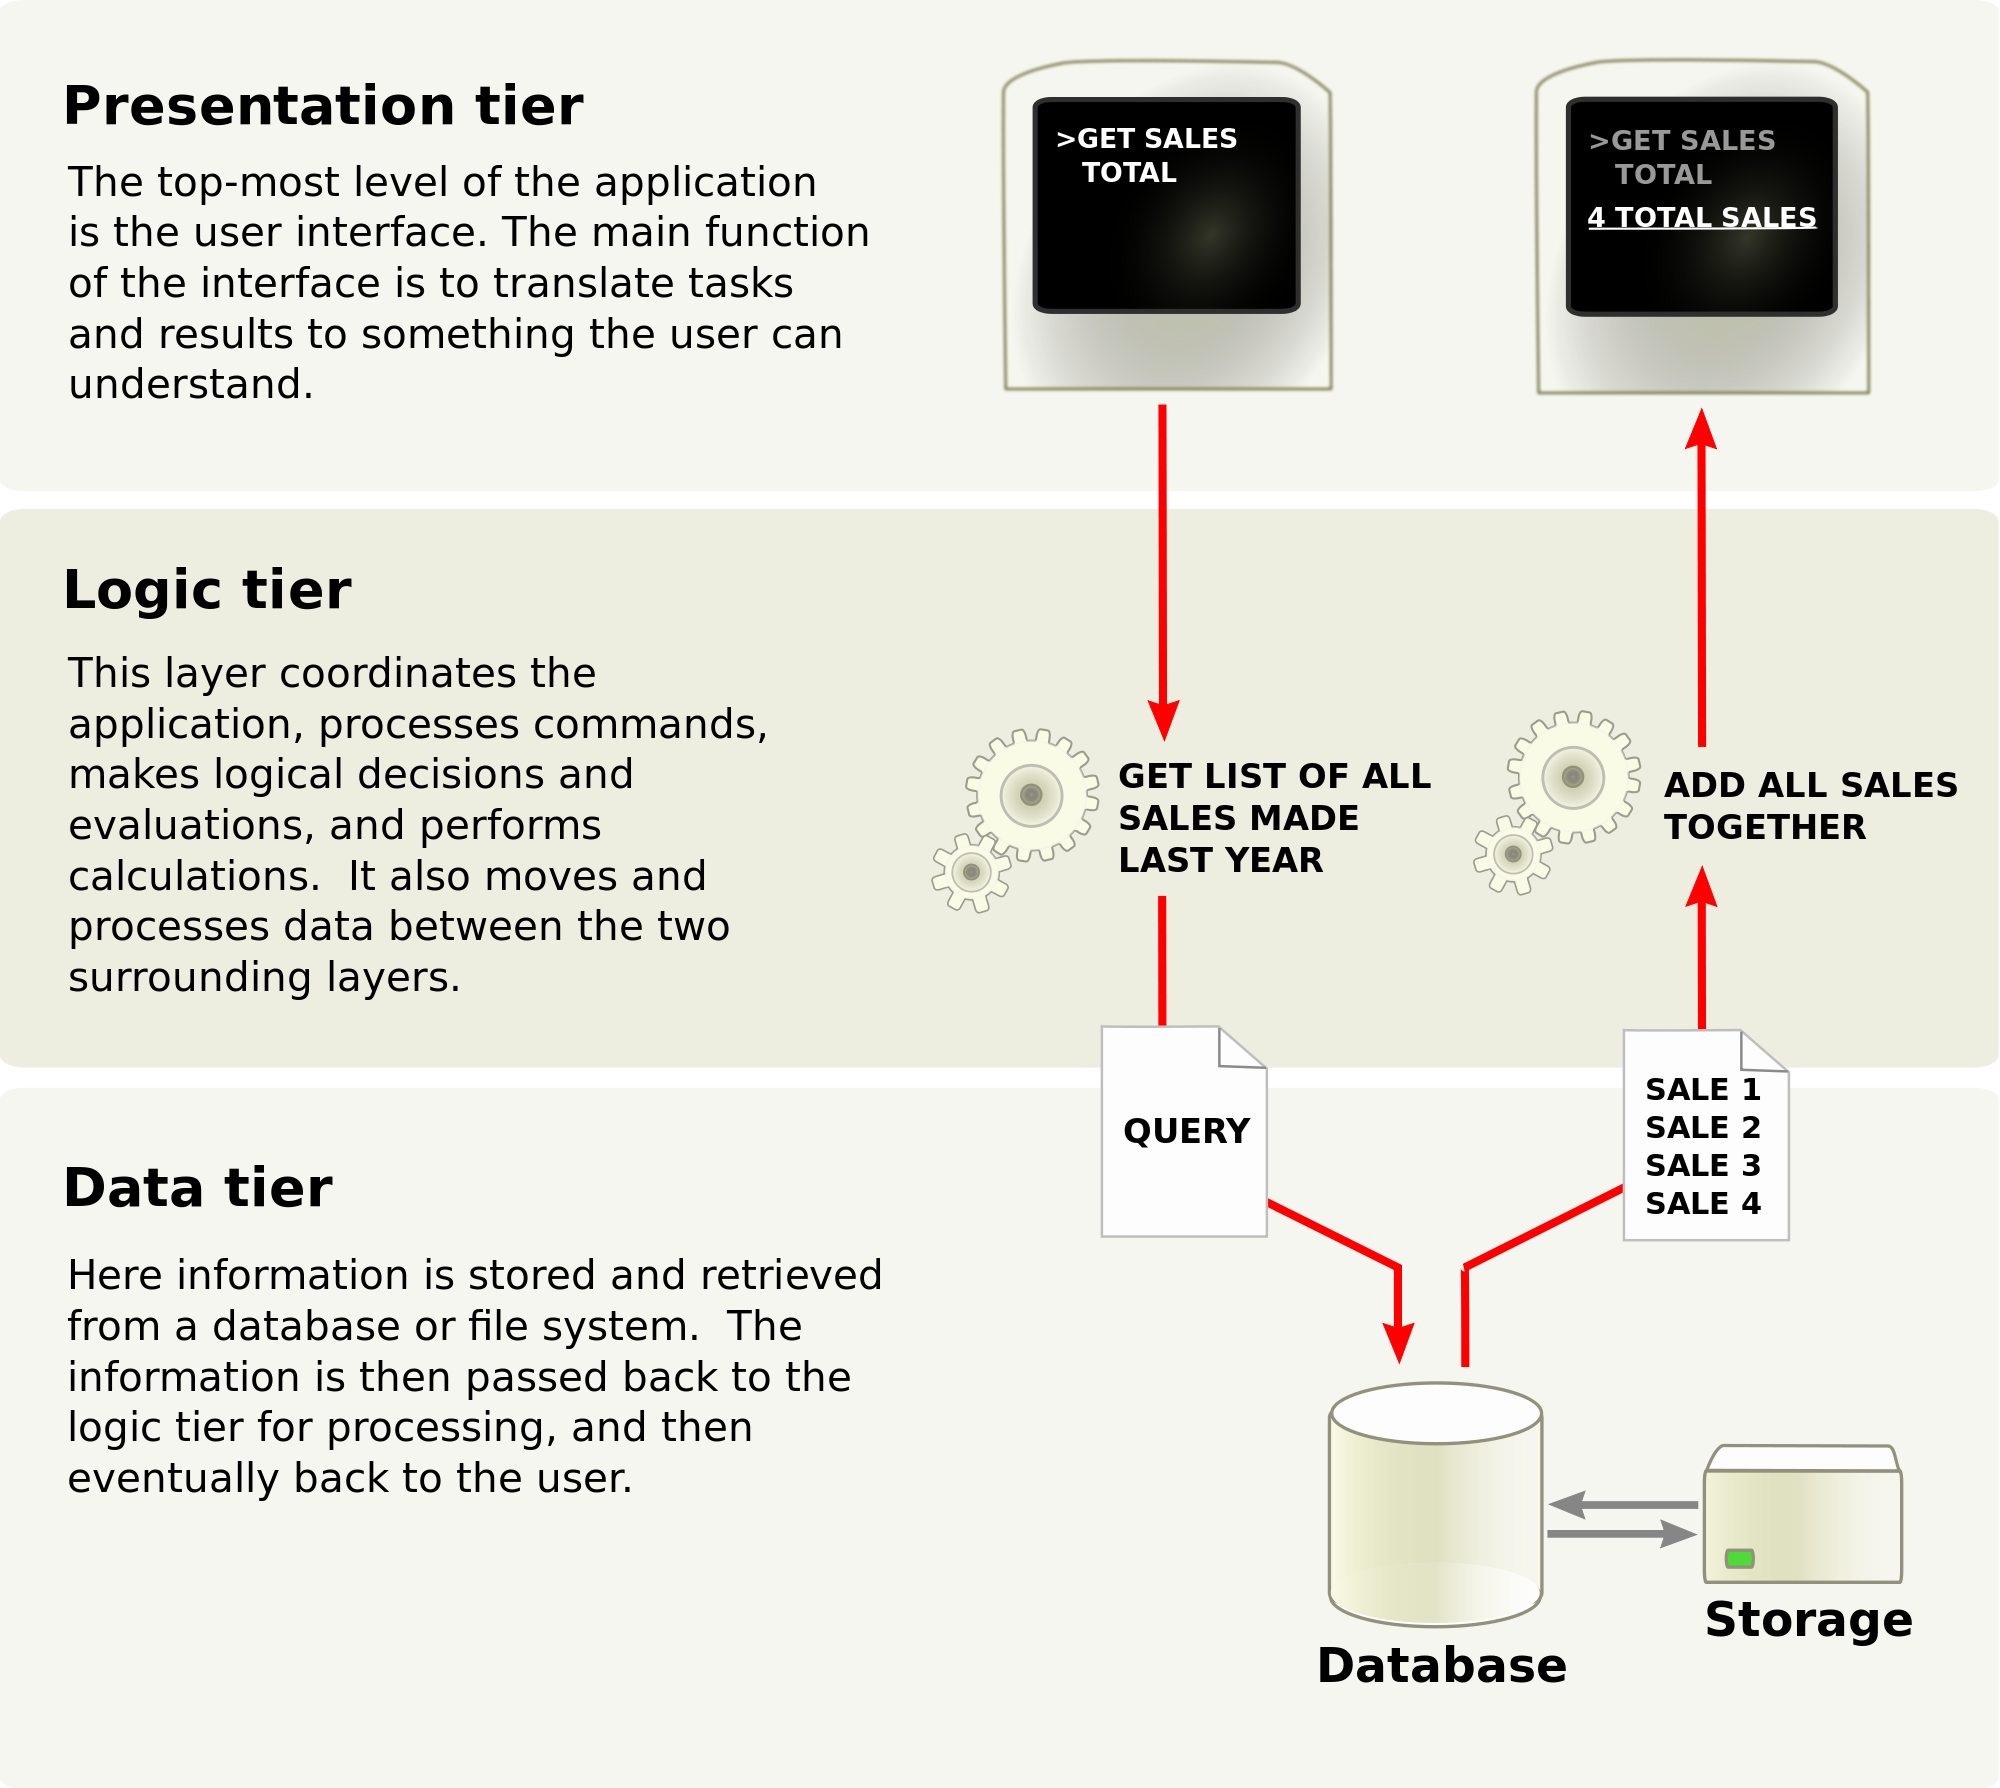
\includegraphics[width = 0.7\textwidth]{billeder/trelagsmodel.png}
\caption{Illustration af trelags-modellen med eksempel af typisk anvendse}\label{fig:3lagsmodel}
\end{figure}
\fixme{ref: til https://en.wikipedia.org/wiki/Multitier\_architecture}\\
De tre lag (Se figur \ref{fig:3lagsmodel}) er som følger: \\
\textit{GUI / Præsentations laget:} Dette lag håndterer præsentationen til bruger. Metoder, der tilhører dette lag, har til formål at skabe brugerfeedback. \\
\textit{Logik laget: } Her håndteres udregninger, data processering og evalueringen. Dette lag fungere ydermere som kommunikationens lag mellem data og præsentationslag. 
\\ \textit{Data laget: } Dette lag beskæftiger sig med data håndtering. Her håndteres kommunikation med hukommelse, eksterne databaser og andet udefrakommende data.

3-lags modellen sikre yderligere at software er logisk struktureret, har høj fleksibilitet og er nem at implementere. (\cite{RefWorks:31})

%\documentclass[a4paper,11pt,fleqn,twoside,openright ]{memoir} 	% Openright aabner kapitler paa hoejresider (openany begge)

%%%% PACKAGES %%%%

% ¤¤ Oversaettelse og tegnsaetning ¤¤ %
\usepackage[utf8]{inputenc}					% Input-indkodning af tegnsaet (UTF8)
\usepackage[danish]{babel}					% Dokumentets sprog
\usepackage[T1]{fontenc}					% Output-indkodning af tegnsaet (T1)
\usepackage{ragged2e,anyfontsize}			% Justering af elementer
\usepackage{fixltx2e}						% Retter forskellige fejl i LaTeX-kernen
																			
% ¤¤ Figurer og tabeller (floats) ¤¤ %
\usepackage{graphicx} 						% Haandtering af eksterne billeder (JPG, PNG, PDF)
\usepackage{multirow}                		% Fletning af raekker og kolonner (\multicolumn og \multirow)
\usepackage{colortbl} 						% Farver i tabeller (fx \columncolor, \rowcolor og \cellcolor)
\usepackage[dvipsnames]{xcolor}				% Definer farver med \definecolor. Se mere: http://en.wikibooks.org/wiki/LaTeX/Colors
\usepackage{flafter}						% Soerger for at floats ikke optraeder i teksten foer deres reference
\let\newfloat\relax 						% Justering mellem float-pakken og memoir
\usepackage{float}							% Muliggoer eksakt placering af floats, f.eks. \begin{figure}[H]
%\usepackage{eso-pic}						% Tilfoej billedekommandoer paa hver side
%\usepackage{wrapfig}						% Indsaettelse af figurer omsvoebt af tekst. \begin{wrapfigure}{Placering}{Stoerrelse}
%\usepackage{multicol}         	        	% Muliggoer tekst i spalter
%\usepackage{rotating}						% Rotation af tekst med \begin{sideways}...\end{sideways}

% ¤¤ Matematik mm. ¤¤
\usepackage{amsmath,amssymb,stmaryrd} 		% Avancerede matematik-udvidelser
\usepackage{mathtools}						% Andre matematik- og tegnudvidelser
\usepackage{textcomp}                 		% Symbol-udvidelser (f.eks. promille-tegn med \textperthousand )
\usepackage{siunitx}						% Flot og konsistent praesentation af tal og enheder med \si{enhed} og \SI{tal}{enhed}
\sisetup{output-decimal-marker = {,}}		% Opsaetning af \SI (DE for komma som decimalseparator) 
\usepackage[version=3]{mhchem} 				% Kemi-pakke til flot og let notation af formler, f.eks. \ce{Fe2O3}
%\usepackage{rsphrase}						% Kemi-pakke til RS-saetninger, f.eks. \rsphrase{R1}

% ¤¤ Referencer og kilder ¤¤ %
\usepackage[danish]{varioref}				% Muliggoer bl.a. krydshenvisninger med sidetal (\vref)
\usepackage{natbib}							% Udvidelse med naturvidenskabelige citationsmodeller
%\usepackage{xr}							% Referencer til eksternt dokument med \externaldocument{<NAVN>}
%\usepackage{glossaries}					% Terminologi- eller symbolliste (se mere i Daleifs Latex-bog)

% ¤¤ Misc. ¤¤ %
\usepackage{listings}						% Placer kildekode i dokumentet med \begin{lstlisting}...\end{lstlisting}
\usepackage{lipsum}							% Dummy text \lipsum[..]
\usepackage[shortlabels]{enumitem}			% Muliggoer enkelt konfiguration af lister
\usepackage{pdfpages}						% Goer det muligt at inkludere pdf-dokumenter med kommandoen \includepdf[pages={x-y}]{fil.pdf}	
\pdfoptionpdfminorversion=6					% Muliggoer inkludering af pdf dokumenter, af version 1.6 og hoejere
\pretolerance=2500 							% Justering af afstand mellem ord (hoejt tal, mindre orddeling og mere luft mellem ord)

\usepackage{calc}
\usepackage{longtable}
\usepackage{xcolor} %Enables user def colors
\usepackage{titletoc} %Enables more TOCs

\newcommand{\shortTOC}{
	\settocdepth{part} 	
	\tableofcontents*{}
	}
	
	\newcommand{\longTOC}{
		\settocdepth{subsection}
		\tableofcontents*{hej}
	}

\definecolor{usDef}{RGB}{180,180,180} 

% Kommentarer og rettelser med \fxnote. Med 'final' i stedet for 'draft' udloeser hver note en error i den faerdige rapport.
\usepackage[footnote,draft,danish,silent,nomargin]{fixme}		


%%%% CUSTOM SETTINGS %%%%

% ¤¤ Marginer ¤¤ %
\setlrmarginsandblock{3.5cm}{2.5cm}{*}		% \setlrmarginsandblock{Indbinding}{Kant}{Ratio}
\setulmarginsandblock{2.5cm}{3.0cm}{*}		% \setulmarginsandblock{Top}{Bund}{Ratio}
\checkandfixthelayout 						% Oversaetter vaerdier til brug for andre pakker

%	¤¤ Afsnitsformatering ¤¤ %
\setlength{\parindent}{0mm}           		% Stoerrelse af indryk
\setlength{\parskip}{3mm}          			% Afstand mellem afsnit ved brug af double Enter
\linespread{1,1}							% Linie afstand

% ¤¤ Litteraturlisten ¤¤ %
\bibpunct[,]{[}{]}{;}{a}{,}{,} 				% Definerer de 6 parametre ved Harvard henvisning (bl.a. parantestype og seperatortegn)
\bibliographystyle{bibtex/harvard}			% Udseende af litteraturlisten.

% ¤¤ Indholdsfortegnelse ¤¤ %
\setsecnumdepth{subsection}		 			% Dybden af nummerede overkrifter (part/chapter/section/subsection)
\maxsecnumdepth{subsection}					% Dokumentklassens graense for nummereringsdybde
\settocdepth{subsection} 					% Dybden af indholdsfortegnelsen

% ¤¤ Lister ¤¤ %
\setlist{
  topsep=0pt,								% Vertikal afstand mellem tekst og listen
  itemsep=-1ex,								% Vertikal afstand mellem items
} 

% ¤¤ Visuelle referencer ¤¤ %
\usepackage[colorlinks]{hyperref}			% Danner klikbare referencer (hyperlinks) i dokumentet.
\hypersetup{colorlinks = true,				% Opsaetning af farvede hyperlinks (interne links, citeringer og URL)
    linkcolor = black,
    citecolor = black,
    urlcolor = black
}

% ¤¤ Opsaetning af figur- og tabeltekst ¤¤ %
\captionnamefont{\small\bfseries\itshape}	% Opsaetning af tekstdelen ('Figur' eller 'Tabel')
\captiontitlefont{\small}					% Opsaetning af nummerering
\captiondelim{. }							% Seperator mellem nummerering og figurtekst
\hangcaption								% Venstrejusterer flere-liniers figurtekst under hinanden
\captionwidth{\linewidth}					% Bredden af figurteksten
\setlength{\belowcaptionskip}{0pt}			% Afstand under figurteksten
		
% ¤¤ Opsaetning af listings ¤¤ %
\definecolor{commentGreen}{RGB}{34,139,24}
\definecolor{stringPurple}{RGB}{208,76,239}

\lstset{language=Matlab,					% Sprog
	basicstyle=\ttfamily\scriptsize,		% Opsaetning af teksten
	keywords={for,if,while,else,elseif,		% Noegleord at fremhaeve
			  end,break,return,case,
			  switch,function},
	keywordstyle=\color{blue},				% Opsaetning af noegleord
	commentstyle=\color{commentGreen},		% Opsaetning af kommentarer
	stringstyle=\color{stringPurple},		% Opsaetning af strenge
	showstringspaces=false,					% Mellemrum i strenge enten vist eller blanke
	numbers=left, numberstyle=\tiny,		% Linjenumre
	extendedchars=true, 					% Tillader specielle karakterer
	columns=flexible,						% Kolonnejustering
	breaklines, breakatwhitespace=true,		% Bryd lange linjer
}

% ¤¤ Navngivning ¤¤ %
\addto\captionsdanish{
	\renewcommand\appendixname{Appendiks}
	\renewcommand\contentsname{Indholdsfortegnelse}	
	\renewcommand\appendixpagename{Appendiks}
	\renewcommand\appendixtocname{Appendiks}
	\renewcommand\cftchaptername{\chaptername~}				% Skriver "Kapitel" foran kapitlerne i indholdsfortegnelsen
	\renewcommand\cftappendixname{\appendixname~}			% Skriver "Appendiks" foran appendiks i indholdsfortegnelsen
}

% ¤¤ Kapiteludssende ¤¤ %

\newif\ifNoChapNumber
\makeatletter
\makechapterstyle{VZ34}{
	\renewcommand\chapternamenum{}
	\renewcommand\printchaptername{}
	\renewcommand\printchapternum{}
	\renewcommand\chapnumfont{\Huge\bfseries}
	\renewcommand\chaptitlefont{\Huge\bfseries\raggedright}
	\renewcommand\printchaptertitle[1]{%
		\begin{tabular}{@{}p{1cm}|!{\quad}p{\textwidth-1cm-2em-4\tabcolsep }}
			\ifNoChapNumber\relax\else\chapnumfont \thechapter\fi
			& \chaptitlefont ##1
		\end{tabular}
		\NoChapNumberfalse
	}
	\renewcommand\printchapternonum{\NoChapNumbertrue}
}
\chapterstyle{VZ34}

% ¤¤ Sidehoved ¤¤ %

\makepagestyle{Uni}							% Definerer sidehoved og sidefod udseende frem til ...
\makepsmarks{Uni}{%
	\createmark{chapter}{left}{shownumber}{}{. \ }
	\createmark{section}{right}{shownumber}{}{. \ }
	\createplainmark{toc}{both}{\contentsname}
	\createplainmark{lof}{both}{\listfigurename}
	\createplainmark{lot}{both}{\listtablename}
	\createplainmark{bib}{both}{\bibname}
	\createplainmark{index}{both}{\indexname}
	\createplainmark{glossary}{both}{\glossaryname}
}
\nouppercaseheads											% Ingen Caps oenskes

\makeevenhead{Uni}{Gruppe 15155}{}{\leftmark}				% Definerer lige siders sidehoved (\makeevenhead{Navn}{Venstre}{Center}{Hoejre})
\makeoddhead{Uni}{\rightmark}{}{Aarhus Universitet}			% Definerer ulige siders sidehoved (\makeoddhead{Navn}{Venstre}{Center}{Hoejre})
\makeevenfoot{Uni}{\thepage}{}{}							% Definerer lige siders sidefod (\makeevenfoot{Navn}{Venstre}{Center}{Hoejre})
\makeoddfoot{Uni}{}{}{\thepage}								% Definerer ulige siders sidefod (\makeoddfoot{Navn}{Venstre}{Center}{Hoejre})
\makeheadrule{Uni}{\textwidth}{0.5pt}						% Tilfoejer en streg under sidehovedets indhold
\makefootrule{Uni}{\textwidth}{0.5pt}{1mm}					% Tilfoejer en streg under sidefodens indhold

\copypagestyle{Unichap}{Uni}								% Sidehoved for kapitelsider defineres som standardsider, men med blank sidehoved
\makeoddhead{Unichap}{}{}{}
\makeevenhead{Unichap}{}{}{}
\makeheadrule{Unichap}{\textwidth}{0pt}
\aliaspagestyle{chapter}{Unichap}							% Den ny style vaelges til at gaelde for chapters
															% ... her
															
\pagestyle{Uni}												% Valg af sidehoved og sidefod (benyt "plain" for ingen sidehoved/fod)


%%%% CUSTOM COMMANDS %%%%

% ¤¤ Billede hack ¤¤ %										% Indsaet figurer nemt med \figur{Stoerrelse}{Fil}{Figurtekst}{Label}
\newcommand{\figur}[4]{
		\begin{figure}[H] \centering
			\includegraphics[width=#1\textwidth]{billeder/#2}
			\caption{#3}\label{#4}
		\end{figure} 
}

% ¤¤ Specielle tegn ¤¤ %
\newcommand{\decC}{^{\circ}\text{C}}
\newcommand{\dec}{^{\circ}}
\newcommand{\m}{\cdot}


%%%% ORDDELING %%%%

\hyphenation{}

\begin{document}
	
%Short TOC


\thispagestyle{empty} % Remove page numbering on this page


\colorbox{usDef}{
	\parbox[t]{1.0\linewidth}{
		\centering \fontsize{30pt}{50pt}\selectfont % The first argument for fontsize is the font size of the text and the second is the line spacing - you may need to play with these for your particular title
		\vspace*{0.7cm} % Space between the start of the title and the top of the grey box
		
		\hfill Remote Ischemic Conditioning\\
		\hfill Udviklingsdokumentation \\
		
		\vspace*{0.7cm} % Space between the end of the title and the bottom of the grey box
	}
}

\vfill % Space between the title box and author information


{\centering \large 
	\hfill Simon Vammen Grønbæk \\
	\hfill Karl-Johan Schmidt\\
	\hfill Aarhus University \\
	\hfill Aarhus School of Engineering\\
	\hfill Efteråret 2015 \\
}

\clearpage % Whitespace to the end of the page	
% Dette er et titelblad designet til videregående uddannelser på et universitet
% Filen kræver:
% Universitetets logo:  AU-logo-DK eller AU-logo-DK
% Synopsis: En fil ved navn synopsis.tex

% Udarbejdet af: Jesper Nørgaard (jesper@noergaard.eu) 10. april 2012

\phantomsection
\pdfbookmark[0]{Titelblad}{titelblad}
\thispagestyle{empty}

\begin{minipage}[t]{0.48\textwidth}
\vspace*{-8pt}			

\includegraphics[height=2.5cm]{billeder/AU-logo-DK}
\end{minipage}
\hfill
\begin{minipage}[t]{0.48\textwidth}
{\small 
\textbf{Ingeniørhøjskolen Aarhus}\\
Finlandsgade 22 \\
8200 Aarhus N \\
Tlf: 8715 0000 \\
http://www.ase.au.dk/}
\end{minipage}

\vspace*{1cm}

\begin{minipage}[t]{0.48\textwidth}
\textbf{Titel:} \\[5pt]\bigskip\hspace{2ex}
Remote Ischemic Conditioning

\textbf{Projekt:} \\[5pt]\bigskip\hspace{2ex}
Bachelor projekt

\textbf{Projektperiode:} \\[5pt]\bigskip\hspace{2ex}
Juli 2015 - December 2015

\textbf{Projektgruppe:} \\[5pt]\bigskip\hspace{2ex}
15155

\textbf{Deltagere:} \\[5pt]\hspace*{2ex}
Simon Vammen Grønbæk\\\hspace*{2ex}
Karl-Johan Schmidt \\\hspace*{2ex}


\textbf{Vejledere:} \\[5pt]\hspace*{2ex}
Peter Johansen \\\bigskip\hspace{2ex}

\textbf{Projektudbyder:} \\[5pt]\hspace*{2ex}
Rolf Blauenfeldt\\\bigskip\hspace{2ex}
\vspace*{4cm}

\textbf{Oplagstal: 10} \\
\textbf{Sidetal: \pageref{SidsteSide}} \\
\textbf{Afsluttet 18-12-2014}

\end{minipage}
\hfill
\begin{minipage}[t]{0.483\textwidth}
	\textbf{Godkendelse:}\vspace{1cm}
\begin{table}[H]
	\centering
	\begin{tabular}{c}
		\underline{\phantom{mmmmmmmmmmmmmm}}  \\
		Karl-Johan Schmidt \vspace{2cm}\\
		\underline{\phantom{mmmmmmmmmmmmmm}} \\
		Simon Vammen Grønbæk \vspace{2cm}	\\
		\underline{\phantom{mmmmmmmmmmmmmm}} \\
		Peter Johansen \vspace{2cm}	\\
		\underline{\phantom{mmmmmmmmmmmmmm}} \\
		Rolf Blauenfeldt \vspace{2cm}	\\
	\end{tabular}
\end{table}
\end{minipage}

\vfill

{\footnotesize\itshape Rapportens indhold er frit tilgængeligt, men offentliggørelse (med kildeangivelse) må kun ske efter aftale med forfatterne.}

% Rapportens indhold er frit tilgængeligt, men offentliggørelse (med kildeangivelse) må kun ske efter aftale med forfatterne.
% The content of the report is freely available, but publication (with source reference) may only take place in agreement with the authors.


\newpage

\startcontents[overall]
\printcontents[overall]{}{-1}{\chapter*{Indholdsfortegnelse}}
\newpage

\chapter*{Indledning}
\addcontentsline{toc}{chapter}{Indledning}
Udviklingsdokumentationen er en samling af skriftlige resultater igennem udviklingsfasen. Dokumentet samler kravspecifikationen, accepttesten, system designet og implementeringen i et fælles dokument. 

\section*{Formål}
Formålet med udviklingsdokumentationen er at beskrive udviklingsfasen og udarbejdelse af dokumentation, som beskriver produktet i hvert udviklingstrin. Et individuelt formål findes under hvert underdokument. 

\section*{Læsevejledning}
Dokumentet består af fire underdokumenter, hhv. kravspecifikation, accepttest, system design og implementering. En individuel læsevejledning findes under hvert underdokument. Hvert dokument har desuden sin egen indholdsfortegnelse. 


\part{Kravspecifikation} \label{part:ks}
\stopcontents[overall]
\startcontents[ks]
\documentclass[11pt]{article}
\usepackage[utf8]{inputenc}  % To control and create table of content
\usepackage{fancyhdr} 	% To create header
\usepackage{dirtytalk} % To create citations
\usepackage{array} % To control and create fixed size tables
\usepackage{longtable}
\usepackage{graphicx}
\graphicspath{ {Illustrationer/} }

\pagestyle{fancy}
\fancyhf{}
\lhead{Kravspecifikation}
\rhead{Version 0.1}
\rfoot{Page \thepage}

\renewcommand*\contentsname{Indholdsfortegnelse}

\begin{document}
	\begin{titlepage}
		\begin{center}
			\Large\textbf{Kravspecifikation}\\
			\large\textit{Version: 0.1}
		\end{center}
	\end{titlepage}
	
	\tableofcontents
	\newpage
	
	\section{Introduktion og baggrund}
	Formålet med dette dokument er at beskrive funktionelle og ikke-funktionelle krav for per konditionerings blodtryks apparatet. De funktionelle krav vil blive beskrevet ved hjælp af fully dressed use case diagrammer. 
	
	Beskrivelse af projektet: 
	
	\say{\textit{Akut blodprop i hjernen (Acute Ischemic Stroke – AIS) er en førende årsag til død og alvorlig handicap hos personer over 60 år.Intravenøs trombolysebehandling administreret indenfor 4,5 time fra symptomdebut er den nuværende bedste medicinske behandling. Grundet sikkerhedshensyn og det snævre tidsvindue er det desværre kun et fåtal af AIS patienterne, der modtager denne behandling. Målet er at opløse blodproppen og genoprette blodforsyning og dermed redde hjernevæv, der lider af iltmangel men endnu ikke er dødt. Om et område af hjernen dør eller står til at redde ved en blodprop afhænger ikke kun af selve blodproppen men også om hjernen er i stand til at få blod via omveje dannet af hjernens små blodkar. Et område af hjernen går til grunde med det samme (infarktkernen). Denne kerne af dødt hjernevæv kan i dagene efter en blodprop sprede sig og vokse. Der er således behov for at kunne beskytte hjernen mod iltmangel og øge andelen af hjernevæv, der overlever en blodprop. Iltmangel induceret periodevis i et fjernt organ (remote ischemic conditioning RIC) kan udføres ved at puste en blodtryksmanchet med afklemning af armen. Konditionering kan leveres som pre, per, og postconditionering, afhængig af om stimulus udøves før iltmangel, under iltmangel men før blodproppen er opløst og endelig efter blodproppen er opløst. Dyrestudier og senest kliniske studier har vist at RIC kan mindske det område af hjertet eller hjernen, der dør ved en blodprop. Det er ikke tilstrækkeligt undersøgt om RIC mindsker risikoen for handicap efter en blodprop i hjernen.}}
	
	\section{System beskrivelse}
	System er beregnet til behandling af patienter med \textit{acute ischemic stroke(AIS)}. Formålet er pre, per og postkonditioning af disse patienter. Systemet skal kunne lave arteriel okklusion i de øverste ydre ekstremiteter. For at sikre tilstrækkelig okklusion, skal det systoliske blodtryk først måles og derefter pumpe cuffen op til plus 25 mmHg over det målet tryk. Som minimum skal der afklemmes med et tryk på 180 mmHg. Okklusionen bliver holdt konstant i 5 minutter, hvor efter trykket lukkes ud der holdes en "pause" på 5 minutter. Denne process gentages ind til konditioneringen er færdig. 

	\section{Funktionelle krav}
	
	%Aktør beskrivelse
		\section{Aktør beskrivelse}
	Systemet har tre aktør og disse er beskrevet nedenfor. Aktørerne skal ses som brugere eller spillere der skal interagere med scenarierne for at de lykkes. 
	
	\begin{center}
		\begin{tabular}{ | m{4cm} | m{8cm}| } 
			\hline
			Aktørnavn& Medicinsk personale  \\ 
			\hline
			Aktørtype & Primær og sekundær \\ 
			\hline
			Beskrivelse af aktør & Aktør som påmontere manchetten og styre konditionering eller person som observere de gemte data fra behandlingsforløb\\ 
			\hline
		\end{tabular}
	\end{center}
	
	\begin{center}
		\begin{tabular}{ | m{4cm} | m{8cm}| } 
			\hline
			Aktørnavn& Patient \\ 
			\hline
			Aktørtype & Sekundær \\ 
			\hline
			Beskrivelse af aktør & En person med AIS som skal konditioneres\\ 
			\hline
		\end{tabular}
	\end{center}
	
	\begin{center}
		\begin{tabular}{ | m{4cm} | m{8cm}| } 
			\hline
			Aktørnavn& Database \\ 
			\hline
			Aktørtype & Sekundær \\ 
			\hline
			Beskrivelse af aktør & Gemmer data og logfiler omkring konditionerings forløb\\ 
			\hline
		\end{tabular}
	\end{center}
	
	\begin{center}
		\begin{tabular}{ | m{4cm} | m{8cm}| } 
			\hline
			Aktørnavn& Bruger \\ 
			\hline
			Aktørtype & Primær \\ 
			\hline
			Beskrivelse af aktør & Person der gør brug af konditioneringsapparatet til okklusionstræning, denne person behøver ikke besidde særlig faglig viden \\ 
			\hline
		\end{tabular}
	\end{center}
	\pagebreak
	
	%Use case 1
	\subsection{Use case 1 - Konditionering}
\begin{center}
		\begin{longtable}{ | p{0.3\textwidth} | p{0.7\textwidth}| } 
			\hline
			Goal& Gennemføre konditioneringsbehandling  \\ 
			\hline
			Initiation &  Medicinsk personale\\
			\hline
			Actors and stakeholders & 
			\begin{itemize}
				\item Medicinsk personale(primær)
				\item Patient (sekundær)
			\end{itemize} \\ 
			\hline
			References & Use case 3 \\ 
			\hline
			Number of concurrent occurrences & En til mange\\ 
			\hline	
			Precondition & 
			\begin{itemize}
				\item Mode switch er sat til “\textit{Konditionering}”
			\end{itemize} \\ 
			\hline
			Postcondition & 
			\begin{itemize}
				\item 5 hele cyklus er gennemført og gemt på hukommelsen
			\end{itemize} \\ 
			\hline
			Main scenario & \begin{enumerate}
				\setlength\itemsep{0cm} % Decrease line distance
				\item \textit{Medicinsk personale} placerer manchetten på patienten
				\item Knappen [Start/Stop] trykkes
				\item Et nyt patient ID genereres
				\subitem[Extension \#1] 
				\item Patient ID’et vises på skærmen
				\item Blodtrykket måles via \textit{use case 3}
				\subitem[Extension \#2]
				\item Blodtrykket vises på displayet og værdien gemmes i hukommelse
				\item Cuffen fyldes med luft til et tryk på 25 mmHG over systolisk tryk (minimum 180 mmHg)
			\end{enumerate} \\ 
			\hline
			Main scenario & \begin{enumerate}
				\setlength\itemsep{0cm} % Decrease line distance
				\setcounter{enumi}{7}				
				\item Tidsstempel gemmes når trykket er opnået
				\item Trykket opretholdes i 5 minutter(Okklusion) og resterende tid vises på displayet
				\item Blodtrykket måles via \textit{use case 3}
				fra punkt 2.
				\item Deflaterer cuffen helt og forbliver i dette stadie i 5 min(Reperfusion) Ved deflation start gemmes tidsstempel. Tid til næste okklusion vises på displayet
				\item Gentag punkt 7-11 (en cyklus) fire gange. Det nuværende cyklus nummer vises i displayet
			\end{enumerate} \\ 
			\hline
			Extensions & [Extension \#1] Et patient ID eksisterer allerede på apparatet. Der genereres ikke noget nyt patient ID.
			
			[Extension \#2] Blodtrykket kunne ikke måles. Gentag use case 3 hvis extension 2 ikke lige er eksekveret. Ellers skrives i display “FEJL kunne ikke måle blodtryk” og use casen stopper    .  \\
			\hline
		\end{longtable}
		
	\end{center}
	\pagebreak
	
	%Use case 2
		\subsection{Use case 2 - Initialiser blodtryksmåling }
	\begin{table}[H]
		\begin{center}
			\begin{tabular}{ | p{0.24\textwidth} | p{0.7\textwidth}| } 
				\hline
				Mål& Mål et blodtryk\\ 
				\hline
				Initiering &  Medicinsk personale\\
				\hline
				Aktører og interessenter & 
				\begin{itemize}
					\item Medicinsk personale(primær)
					\item Patient (sekundær)
				\end{itemize} \\ 
				\hline
				Referencer & Mål blodtryk(UC3) \\ 
				\hline
				Antal samtlige forekomster & En til mange\\ 
				\hline	
				Startbetingelser & 
				\begin{itemize}
					\item Manchetten er placeret på armen
					\item Mode switch er sat til “\textit{Konditionering}”
				\end{itemize} \\ 
				\hline
				Slutbetingelser & 
				\begin{itemize}
					\item Patientens blodtryk er målt
				\end{itemize} \\ 
				\hline
				Normal forløb & \begin{enumerate}
					\setlength\itemsep{0cm} % Decrease line distance
					\item Brugeren trykker på [Mål blodtryk]
					\item Et nyt patient ID genereres
					\subitem [Undtagelse \#1] 
					\item Patient ID’et vises på skærmen
					\item Blodtrykket måles via \textit{use case 3}
					\subitem [Undtagelse \#2]
				\end{enumerate} \\ 
				\hline
				Undtagelser &  [Undtagelse \#1] Et patient ID eksisterer allerede på apparatet. Der genereres ikke noget nyt patient ID.
				
				[Undtagelse \#2] Blodtrykket kunne ikke måles. Gentag use case 3 hvis undtagelse 2 ikke er blevet eksekveret inden for 2 minutter. Ellers skrives i display “FEJL kunne ikke måle blodtryk” og use casen stopper\\ 
				\hline
				
			\end{tabular}
		\end{center}
		\caption{\textit{Fully dressed} use case diagram over use case 2}
			\end{table}
		\newpage
	
	%Use case 3
		\subsection{Use case 3 - Mål blodtryk}
	\begin{table}[H]
		\begin{center}
			\begin{tabular}{ | p{0.24\textwidth} | p{0.7\textwidth}| } 
				\hline
				Mål & Mål et systolisk, diastolisk og middel(MAP) tryk\\ 
				\hline
				Initiering &  Konditionering (UC1) eller Initialiser blodtryksmåling (UC2)\\
				\hline
				Aktører og interessenter & - \\
				\hline
				Referencer & - \\ 
				\hline
				Antal samtlige forekomster & En til mange\\ 
				\hline	
				Startbetingelser & 
				\begin{itemize}
					\item Patient ID er oprettet
					\item Manchetten er placeret på armen
					\item Mode switch er sat til “\textit{Konditionering}”
				\end{itemize} \\ 
				\hline
				Slutbetingelser & 
				\begin{itemize}
					\item Blodtrykket er mål
				\end{itemize} \\ 
				\hline
				Normal forløb & \begin{enumerate}
					\setlength\itemsep{0cm} % Decrease line distance
					\item Manchetten fyldes til tryk over systolisk niveau 
					\item Luften lukkes gradvist ud og det systoliske tryk registreres 
					\item Middel trykket (MAP) måles 
					\item Det diastoliske tryk udregnes ud fra systole og MAP 
					\item Blodtrykket vises på skærmen og værdien gemmes i hukommelsen med et tidsstempel 
				\end{enumerate} \\ 
				\hline
				Undtagelser & -\\ 
				\hline
			\end{tabular}
		\end{center}
			\caption{\textit{Fully dressed} use case diagram over use case 3}
			\end{table}
			\newpage
	
	%Use case 4
		\subsection{Use case 4 - Overfør data}
	\begin{table}[H]
		\begin{center}
			\begin{tabular}{ | p{0.24\textwidth} | p{0.7\textwidth}| } 
				\hline
				Mål & Eksportér data fra blodtryksapparat til databasen\\ 
				\hline
				Initiering &  Medicinsk personale\\
				\hline
				Aktører og interessenter & 
				\begin{itemize}
					\item Medicinsk personale(primær)
					\item Patient (sekundær)
				\end{itemize} \\ 
				\hline
				Referencer & - \\ 
				\hline
				Antal samtlige forekomster & Én pr behandlingsforløb \\ 
				\hline	
				Startbetingelser & 
				\begin{itemize}
					\item Der eksisterer en logfil på hukommelsen
				\end{itemize} \\ 
				\hline
				Slutbetingelser & 
				\begin{itemize}
					\item Logfilen er overført til database
					\item Blodtryksapparat udstyres med formateret hukommelse og klar til næste patient
				\end{itemize} \\ 
				\hline
				Normal forløb & \begin{enumerate}
					\setlength\itemsep{0cm} % Decrease line distance
					\item Tag SD kortet ud af blodtryksapparatet 
					\item Sæt SD kortet i computeren og overfør filen 
					\item Formatér SD kortet
					\item Sæt SD kortet tilbage i konditioneringsapparatet 
				\end{enumerate} \\ 
				\hline
				Undtagelser & -\\ 
				\hline
			\end{tabular}
		\end{center}
		
			\caption{\textit{Fully dressed} use case diagram over use case 4}
		\end{table}
			\newpage
	
	%UseCase 5
		\subsection{Use case 5 - Sikkerhedskontrol med pulsoximeter}
		\begin{center}
			\begin{tabular}{ | p{0.3\textwidth} | p{0.7\textwidth}| } 
				\hline
				Mål & Sikre at patientens kredsløb tåler konditionering \\ 
				\hline
				Initiering &  Konditionering (UC1)\\
				\hline
				Aktører og interessenter & 
				\begin{itemize}
					\item Patient (sekundær)
				\end{itemize} \\ 
				\hline
				Referencer & - \\ 
				\hline
				Antal samtlige forekomster & En til mange \\ 
				\hline	
				Startbetingelser & 
				\begin{itemize}
					\item Konditionering (UC1) igangværende
					\item Pulsoximeteret er monteret på patients finger
					\item Patient har gennemført én afklemnings cyklus
 				\end{itemize} \\ 
				\hline
				Slutbetingelser & 
				\begin{itemize}
					\item Patients tilstand er bestemt 
				\end{itemize} \\ 
				\hline
				Normal forløb & \begin{enumerate}
					\setlength\itemsep{0cm} % Decrease line distance
					\item Saturation detekteres
					\item Saturation gemmes på SD-kort
					\item Saturation er tilfredsstillende
					\subitem [Undtagelse \#1.1][Undtagelse \#1.2]
					\item Behandlingen kan fortsætte
				\end{enumerate} \\ 
				\hline
				Undtagelser &  [Undtagelse \#1.1] Tegn på dårlig kredsløb: Blodtryksapparatet stopper konditionerings forløbet 
				[Undtagelse \#1.2] Kør use case 7\\ 
				\hline
			\end{tabular}
		\end{center}
			\pagebreak
	
	%UseCase 6
		\subsection{Use case 6 - Okklusionstræning}
		\begin{center}
			\begin{tabular}{ | p{0.3\textwidth} | p{0.7\textwidth}| } 
				\hline
				Goal& Gennemføre okklusion af venøs kredsløb under træning  \\ 
				\hline
				Initiation &  Bruger\\
				\hline
				Actors and stakeholders & 
				\begin{itemize}
					\item Bruger (primær)
				\end{itemize} \\ 
				\hline
				References & - \\ 
				\hline
				Number of concurrent occurrences & En pr træningspas \\ 
				\hline	
				Precondition & 
				\begin{itemize}
					\item Mode switch er sat til  “\textit{okklusionstræning}”
 				\end{itemize} \\ 
				\hline
				Postcondition & 
				\begin{itemize}
					\item Okklusions træningssæt gennemført
				\end{itemize} \\ 
				\hline
				Main scenario & \begin{enumerate}
					\setlength\itemsep{0cm} % Decrease line distance
					\item Montere manchetten på arm/ben
					\item Tryk på knap [Start/Stop]
					\item Manchetten pumpes op til 100mmHg
					\item Træningssættet begyndes og trykkes holdes konstant på 100mmHg (+/-10mmHg)
					\item Tryk på knap [Stop]
					\item Manchetten deflateres
				\end{enumerate} \\ 
				\hline
				Extensions & - \\ 
				\hline
			\end{tabular}
		\end{center}
	\pagebreak
		
	
	%UseCase 7
		\subsection{Use case 7 - Afbryd}
	\begin{table}[H]
			\begin{center}
			\begin{tabular}{ | p{0.3\textwidth} | p{0.7\textwidth}| } 
				\hline
				Mål & Tømme manchetten for luft og afbryde nuværende procedure \\ 
				\hline
				Initiering &  Medicinsk personale, Patient\\
				\hline
				Aktører og interessenter & 
				\begin{itemize}
					\item Medicinsk personale 
					\item Bruger 
				\end{itemize} \\ 
				\hline
				Referencer & Konditionering (UC1) og Mål blodtryk (UC3) \\ 
				\hline
				Antal samtlige forekomster & En til mange \\ 
				\hline	
				Startbetingelser & 
				\begin{itemize}
					\item Konditionering (UC1) og Mål blodtryk (UC3) er igangværende 
 				\end{itemize} \\ 
				\hline
				Slutbetingelser & 
				\begin{itemize}
					\item Behandlingen er afbrudt og manchetten er tom for luft
				\end{itemize} \\ 
				\hline
				Normal forløb & \begin{enumerate}
					\setlength\itemsep{0cm} % Decrease line distance
					\item Brugeren trykker på knappen [Start/Stop konditionering]
					\item Den igangværende use case afbrydes
					\item Manchetten tømmes for luft og tidsstempel med “\textit{Gennemført afklemning} = false” gemmes i hukommelsen
					\subitem[Undtagelse \#1]
				\end{enumerate} \\ 
				\hline
				Undtagelser & [Undtagelse \#1] Use case 6 er aktiv: ingen data gemmes i hukommelsen. \\ 
				\hline
			\end{tabular}
		\end{center}
			\caption{\textit{Fully dressed} use case diagram over use case 7}
		\end{table}
	\newpage

		
	
	%UseCase8
		\subsection{Use case 8 - Setup}
		\begin{table}[H]
				\begin{center}
			\begin{tabular}{ | p{0.24\textwidth} | p{0.7\textwidth}| } 
				\hline
				Mål & Ændre konditioneringsforholdene \\ 
				\hline
				Initiation &  Medicinsk personale\\
				\hline
				Aktører og interessenter & 
				\begin{itemize}
					\item Medicinsk personale 
				\end{itemize} \\ 
				\hline
				Referencer & Illustration over setup \\ 
				\hline
				Antal samtlige forekomster & En til mange \\ 
				\hline	
				Startbetingelser & 
				\begin{itemize}
					\item Mode switch er sat til “\textit{setup}” 
					\item Displayet er ændret til setup
 				\end{itemize} \\ 
				\hline
				Slutbetinglser & 
				\begin{itemize}
					\item Cyklus længden og/eller antallet er cyklusser er ændret
				\end{itemize} \\ 
				\hline
				Normal forløb & \begin{enumerate}
					\setlength\itemsep{0cm} % Decrease line distance
					\item Brugeren trykker på knappen [Mål blodtryk]  for at vælge \textit{Tid pr cyklus}
					\item Bruger trykker på knappen [Start/Stop] for at ændre \textit{Tid pr cyklus}
					\item Bruger trykker på knappen [Mål blodtryk]  for at gemme ændringen
					\item Bruger trykker på knappen [Start/Stop] for at navigere til \textit{Antal cyklusser}
					\item Ved knap tryk på [Mål blodtryk]  vælges \textit{Antal cyklusser}
					\item Ved knap tryk på [Start/Stop] ændre \textit{Antal cyklusser}
					\item Brugeren trykker på knappen [Mål blodtryk] for at gemme ændringen
				\end{enumerate} \\ 
				\hline
				Undtagelser & -  \\ 
				\hline
			\end{tabular}
		\end{center}

			\caption{\textit{Fully dressed} use case diagram over use case 8}
		\end{table}
			\newpage

	
	\section{Ikke-funktionelle krav }
	
	\subsection{Microcontroller}
	\begin{enumerate}
		\setlength\itemsep{0cm}
		\item Atmega32
		\end{enumerate}
	
	\subsection{Filformat og opsætning}
	\begin{enumerate}
		\setlength\itemsep{0cm} % Decrease line distance
		\item Data logged i formatet .csv og hver kolonne indeholder følgende værdier og enheder: 
		\begin{enumerate}
			\item Tidsstempel [yy:mm:dd hh:mm:ss]
			\item Afklemningstryk [mmHg]
			\item Gennemført afklemning [Boolean]
			\item Systoliske blodtryk [mmHg]
			\item Middelblodtryk (MAP) [mmHg]
			\item Diastolisk blodtryk [mmHg]
		\end{enumerate}
		\item Der oprettet én fil pr patient, med filnavn tilsvarende det unikke patient ID
	\end{enumerate}
	
	\subsection{Patient ID}
	\begin{enumerate}
		\setlength\itemsep{0cm} % Decrease line distance
		\item Består af karaktererne A-Z og tallene 0-9
		\begin{enumerate}
			\item ID’et er fem karakterer lang: ***** svarende til 60 millioner kombinationer
			\item ID’et er ikke case sensitiv
		\end{enumerate}
	\end{enumerate}
	
	
	\subsection{Hukommelse}
	\begin{enumerate}
		\setlength\itemsep{0cm} % Decrease line distance
		\item Information lagres på micro SDSC af typen:
		\begin{enumerate}
			\item Class 4
			\item Fil system [fat32] og minimum 128mb
		\end{enumerate}
	\end{enumerate}
	
	\subsection{Forsyning}
	\begin{enumerate}
		\setlength\itemsep{0cm} % Decrease line distance
		\item Konditionerings apparatet skal forsynes med 12V, min 2A
		\begin{enumerate}
			\item DC-connector (angiv diameter) 
			\item 8 stk AAA batterier (1,5V)
		\end{enumerate}
	\end{enumerate}
	
	%User interface 
	\section{User interface}
User interface består overordnede af en skærm og 2 knapper. En knap til at start og stoppe funktioner og en knap til at måle blodtryk. Til brugerfeedback er der en display hvorpå trykket, patient ID, resterende tid og antallet af gennemførte cyklusser vises. Apparatet betjenes i tre forskellige stadier “Konditionering, Okklusion og setup”. Disse tre stadier er beskrevet med hver siden illustration nedenfor. For at skifte mellem disse stadier er der en mode switch på bagsiden af apparatet, den er også beskrevet nedenfor: 

\subsection{Konditionering}
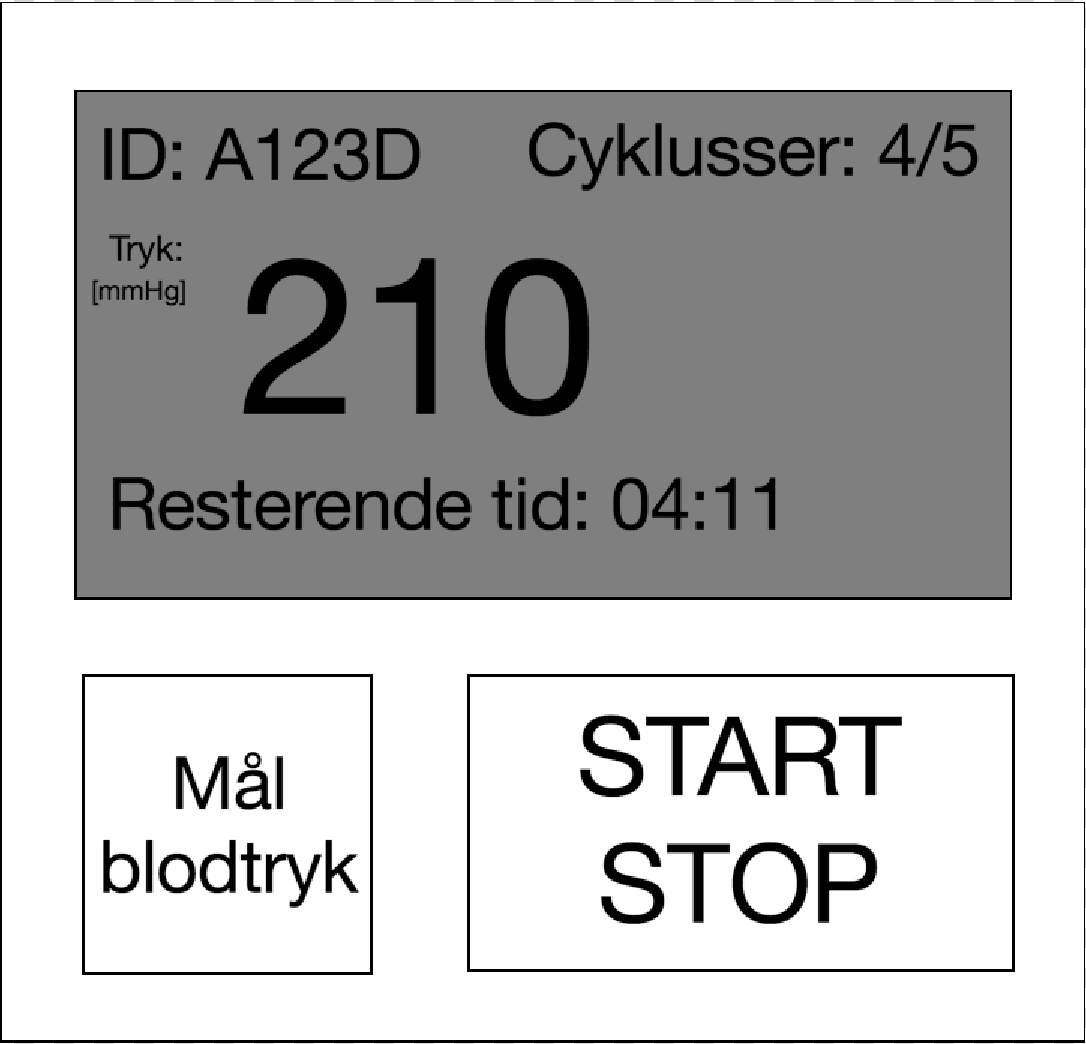
\includegraphics[width=\textwidth]{Illustrationer/KonditioneringGUI}
\subsection{Okklusion}
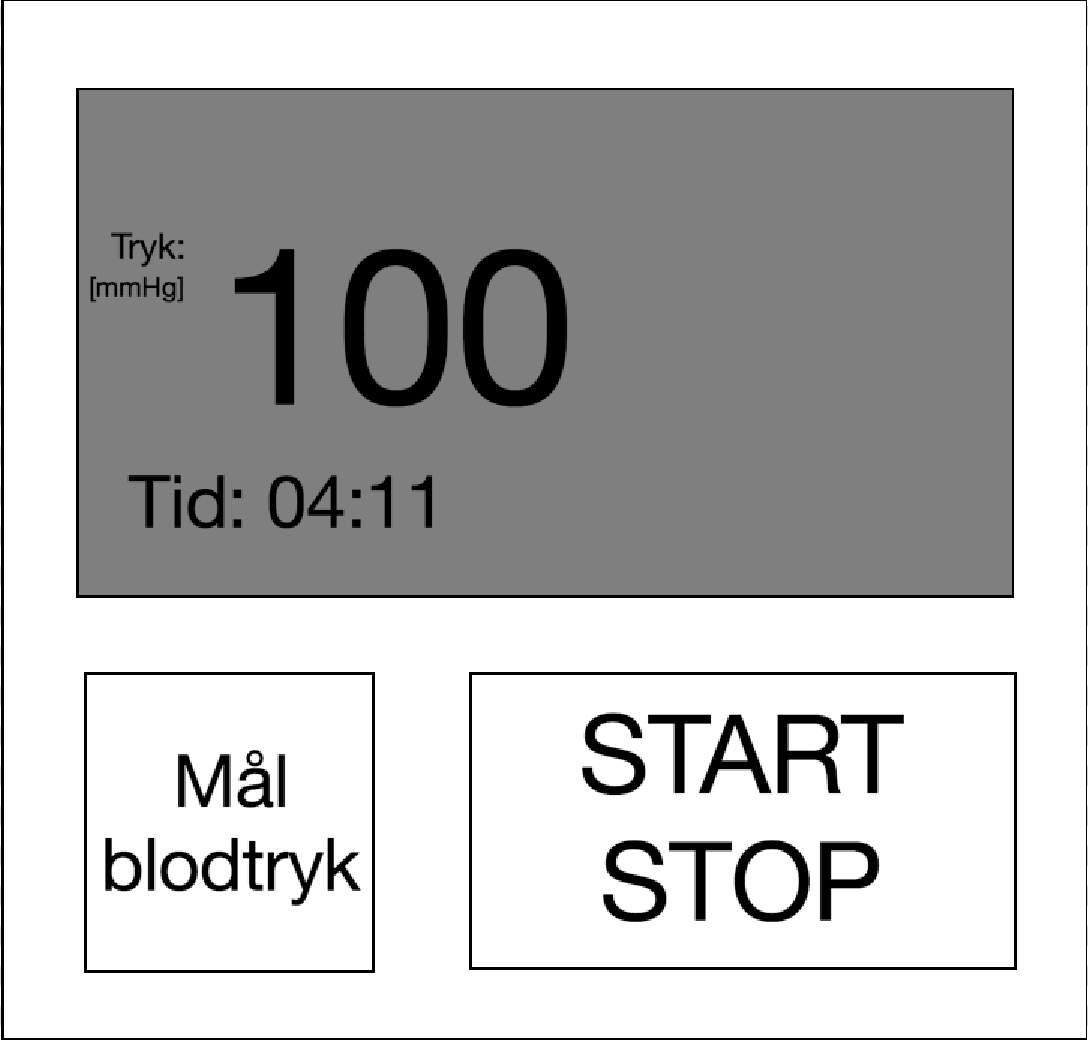
\includegraphics[width=\textwidth]{Illustrationer/OkklusionGUI}

\subsection{Setup}
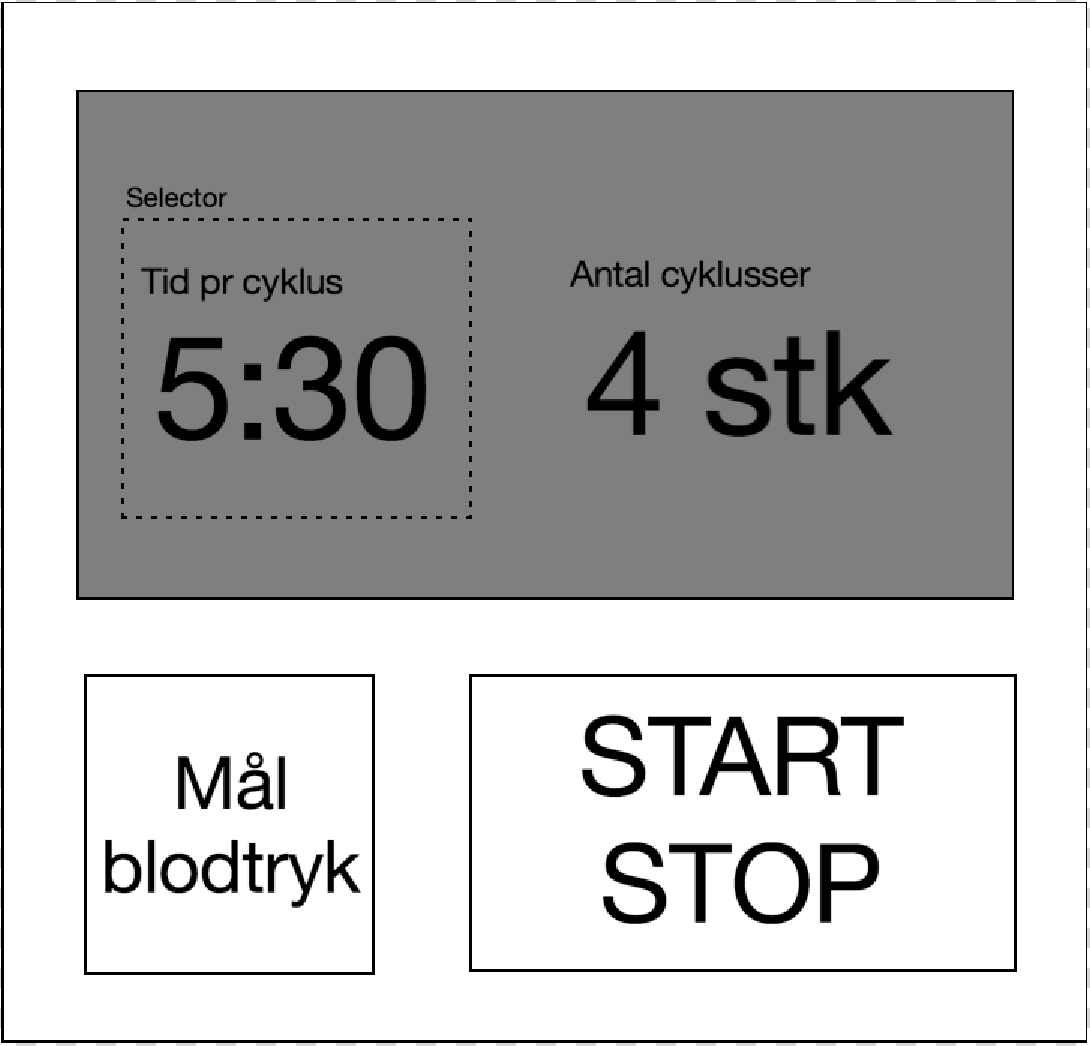
\includegraphics[width=\textwidth]{Illustrationer/SetupGUI}

\subsection{Bagside}
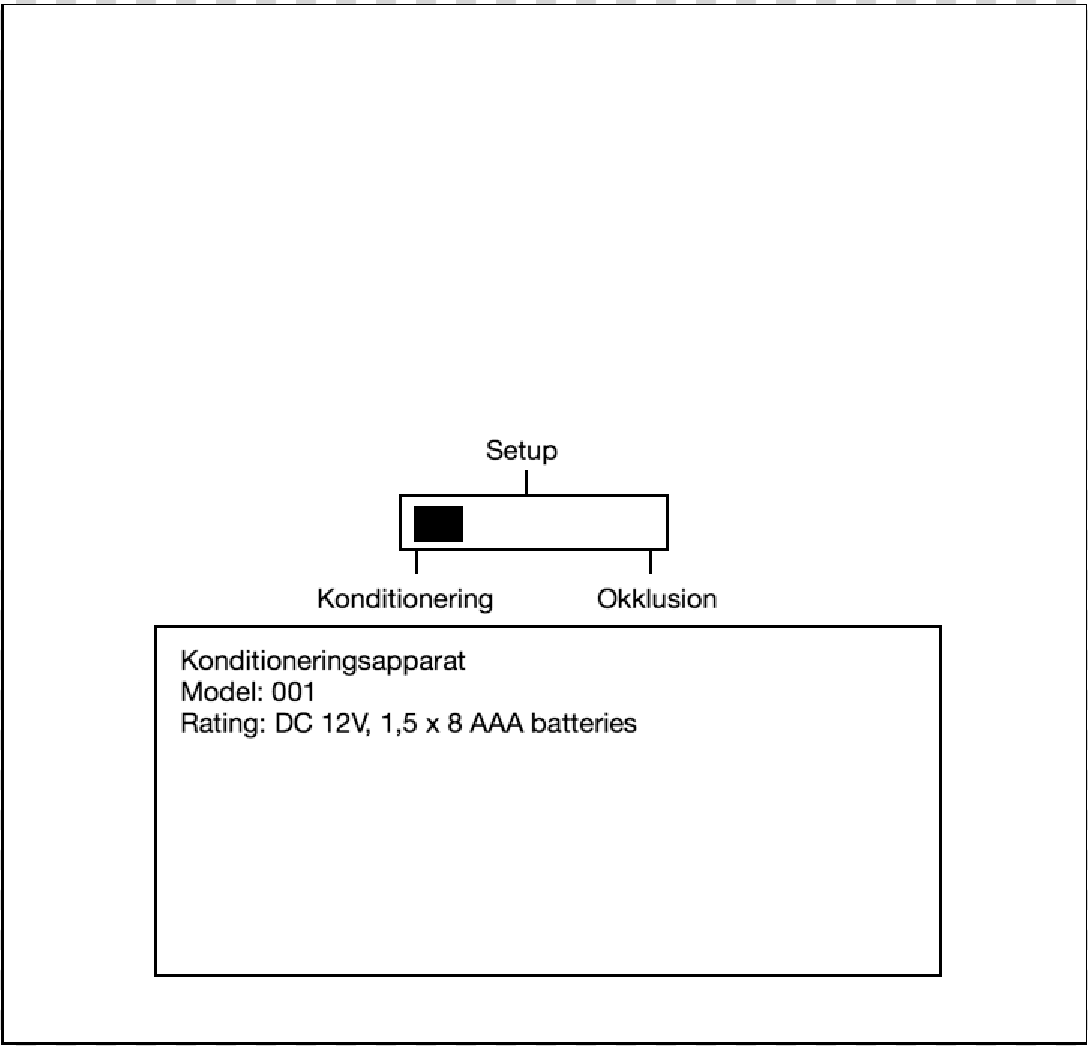
\includegraphics[width=\textwidth]{Illustrationer/BagsideGUI}

	
	
\end{document}
\stopcontents[ks]
\resumecontents[overall]
\newpage

\part{Accepttest} \label{part:at}
\stopcontents[overall]
\startcontents[at]
\documentclass[11pt]{article}
\usepackage[utf8]{inputenc}  % To control and create table of content
\usepackage{fancyhdr} 	% To create header
\usepackage{dirtytalk} % To create citations
\usepackage{array} % To control and create fixed size tables
\usepackage{longtable}
\usepackage{graphicx}
\usepackage{enumitem}
\graphicspath{ {Illustrationer/} }

\pagestyle{fancy}
\fancyhf{}
\lhead{Kravspecifikation}
\rhead{Version 0.1}
\rfoot{Page \thepage}

\renewcommand*\contentsname{Indholdsfortegnelse}

\begin{document}
	\begin{titlepage}
		\begin{center}
			\Large\textbf{Accepttest}\\
			\large\textit{Version: 0.1}
		\end{center}
	\end{titlepage}
	
	\tableofcontents
	\newpage
	
	\section{Funktionelle krav}
	
		\begin{center}
			\begin{tabular}{ | m{3cm} | m{3cm}| m{3cm}| m{3cm}| }
			\hline
			Krav nr.: & Forventet resultat & Test metode & Resultat  \\
			\hline
		    &  &  &   \\
			\hline
			&  &  &  \\
			\hline
			&  &  &  \\
			\hline
			&  &  &   \\
			\hline
			&  &  &  \\
			\hline
			&  &  &  \\
			\hline
			&  &  &   \\
			\hline
			&  &  &  \\
			\hline
			&  &  &  \\
			\hline
		\end{tabular}
		\end{center}

	
	\end{document}
\stopcontents[at]
\resumecontents[overall]
\newpage

\part{ System design} \label{part:sd}
\stopcontents[overall]
\startcontents[sd]
\documentclass[a4paper,11pt,fleqn,twoside,openright ]{memoir} 	% Openright aabner kapitler paa hoejresider (openany begge)

%%%% PACKAGES %%%%

% ¤¤ Oversaettelse og tegnsaetning ¤¤ %
\usepackage[utf8]{inputenc}					% Input-indkodning af tegnsaet (UTF8)
\usepackage[danish]{babel}					% Dokumentets sprog
\usepackage[T1]{fontenc}					% Output-indkodning af tegnsaet (T1)
\usepackage{ragged2e,anyfontsize}			% Justering af elementer
\usepackage{fixltx2e}						% Retter forskellige fejl i LaTeX-kernen

% ¤¤ Figurer og tabeller (floats) ¤¤ %
\usepackage{graphicx} 						% Haandtering af eksterne billeder (JPG, PNG, PDF)
\usepackage{multirow}                		% Fletning af raekker og kolonner (\multicolumn og \multirow)
\usepackage{colortbl} 						% Farver i tabeller (fx \columncolor, \rowcolor og \cellcolor)
\usepackage[dvipsnames]{xcolor}				% Definer farver med \definecolor. Se mere: http://en.wikibooks.org/wiki/LaTeX/Colors
\usepackage{flafter}						% Soerger for at floats ikke optraeder i teksten foer deres reference
\let\newfloat\relax 						% Justering mellem float-pakken og memoir
\usepackage{float}							% Muliggoer eksakt placering af floats, f.eks. \begin{figure}[H]
%\usepackage{eso-pic}						% Tilfoej billedekommandoer paa hver side
%\usepackage{wrapfig}						% Indsaettelse af figurer omsvoebt af tekst. \begin{wrapfigure}{Placering}{Stoerrelse}
%\usepackage{multicol}         	        	% Muliggoer tekst i spalter
%\usepackage{rotating}						% Rotation af tekst med \begin{sideways}...\end{sideways}

% ¤¤ Matematik mm. ¤¤
\usepackage{amsmath,amssymb,stmaryrd} 		% Avancerede matematik-udvidelser
\usepackage{mathtools}						% Andre matematik- og tegnudvidelser
\usepackage{textcomp}                 		% Symbol-udvidelser (f.eks. promille-tegn med \textperthousand )
\usepackage{siunitx}						% Flot og konsistent praesentation af tal og enheder med \si{enhed} og \SI{tal}{enhed}
\sisetup{output-decimal-marker = {,}}		% Opsaetning af \SI (DE for komma som decimalseparator) 
\usepackage[version=3]{mhchem} 				% Kemi-pakke til flot og let notation af formler, f.eks. \ce{Fe2O3}
%\usepackage{rsphrase}						% Kemi-pakke til RS-saetninger, f.eks. \rsphrase{R1}

% ¤¤ Referencer og kilder ¤¤ %
\usepackage[danish]{varioref}				% Muliggoer bl.a. krydshenvisninger med sidetal (\vref)
\usepackage{natbib}							% Udvidelse med naturvidenskabelige citationsmodeller
%\usepackage{xr}							% Referencer til eksternt dokument med \externaldocument{<NAVN>}
%\usepackage{glossaries}					% Terminologi- eller symbolliste (se mere i Daleifs Latex-bog)

% ¤¤ Misc. ¤¤ %
\usepackage{listings}						% Placer kildekode i dokumentet med \begin{lstlisting}...\end{lstlisting}
\usepackage{lipsum}							% Dummy text \lipsum[..]
\usepackage[shortlabels]{enumitem}			% Muliggoer enkelt konfiguration af lister
\usepackage{pdfpages}						% Goer det muligt at inkludere pdf-dokumenter med kommandoen \includepdf[pages={x-y}]{fil.pdf}	
\pdfoptionpdfminorversion=6					% Muliggoer inkludering af pdf dokumenter, af version 1.6 og hoejere
\pretolerance=2500 							% Justering af afstand mellem ord (hoejt tal, mindre orddeling og mere luft mellem ord)

\usepackage{calc}
\usepackage{pdflscape}
\usepackage{longtable}
\definecolor{usDef}{RGB}{180,180,180}


% Kommentarer og rettelser med \fxnote. Med 'final' i stedet for 'draft' udloeser hver note en error i den faerdige rapport.
\usepackage[footnote,draft,danish,silent,nomargin]{fixme}		


%%%% CUSTOM SETTINGS %%%%

% ¤¤ Marginer ¤¤ %
\setlrmarginsandblock{3.5cm}{2.5cm}{*}		% \setlrmarginsandblock{Indbinding}{Kant}{Ratio}
\setulmarginsandblock{2.5cm}{3.0cm}{*}		% \setulmarginsandblock{Top}{Bund}{Ratio}
\checkandfixthelayout 						% Oversaetter vaerdier til brug for andre pakker

%	¤¤ Afsnitsformatering ¤¤ %
\setlength{\parindent}{0mm}           		% Stoerrelse af indryk
\setlength{\parskip}{3mm}          			% Afstand mellem afsnit ved brug af double Enter
\linespread{1,1}							% Linie afstand

% ¤¤ Litteraturlisten ¤¤ %
\bibpunct[,]{[}{]}{;}{a}{,}{,} 				% Definerer de 6 parametre ved Harvard henvisning (bl.a. parantestype og seperatortegn)
\bibliographystyle{bibtex/harvard}			% Udseende af litteraturlisten.

% ¤¤ Indholdsfortegnelse ¤¤ %
\setsecnumdepth{subsection}		 			% Dybden af nummerede overkrifter (part/chapter/section/subsection)
\maxsecnumdepth{subsection}					% Dokumentklassens graense for nummereringsdybde
\settocdepth{subsection} 					% Dybden af indholdsfortegnelsen

% ¤¤ Lister ¤¤ %
\setlist{
	topsep=0pt,								% Vertikal afstand mellem tekst og listen
	itemsep=-1ex,								% Vertikal afstand mellem items
} 

% ¤¤ Visuelle referencer ¤¤ %
\usepackage[colorlinks]{hyperref}			% Danner klikbare referencer (hyperlinks) i dokumentet.
\hypersetup{colorlinks = true,				% Opsaetning af farvede hyperlinks (interne links, citeringer og URL)
	linkcolor = black,
	citecolor = black,
	urlcolor = black
}

% ¤¤ Opsaetning af figur- og tabeltekst ¤¤ %
\captionnamefont{\small\bfseries\itshape}	% Opsaetning af tekstdelen ('Figur' eller 'Tabel')
\captiontitlefont{\small}					% Opsaetning af nummerering
\captiondelim{. }							% Seperator mellem nummerering og figurtekst
\hangcaption								% Venstrejusterer flere-liniers figurtekst under hinanden
\captionwidth{\linewidth}					% Bredden af figurteksten
\setlength{\belowcaptionskip}{0pt}			% Afstand under figurteksten

% ¤¤ Opsaetning af listings ¤¤ %
\definecolor{commentGreen}{RGB}{34,139,24}
\definecolor{stringPurple}{RGB}{208,76,239}

\lstset{language=Matlab,					% Sprog
	basicstyle=\ttfamily\scriptsize,		% Opsaetning af teksten
	keywords={for,if,while,else,elseif,		% Noegleord at fremhaeve
		end,break,return,case,
		switch,function},
	keywordstyle=\color{blue},				% Opsaetning af noegleord
	commentstyle=\color{commentGreen},		% Opsaetning af kommentarer
	stringstyle=\color{stringPurple},		% Opsaetning af strenge
	showstringspaces=false,					% Mellemrum i strenge enten vist eller blanke
	numbers=left, numberstyle=\tiny,		% Linjenumre
	extendedchars=true, 					% Tillader specielle karakterer
	columns=flexible,						% Kolonnejustering
	breaklines, breakatwhitespace=true,		% Bryd lange linjer
}

% ¤¤ Navngivning ¤¤ %
\addto\captionsdanish{
	\renewcommand\appendixname{Appendiks}
	\renewcommand\contentsname{Indholdsfortegnelse}	
	\renewcommand\appendixpagename{Appendiks}
	\renewcommand\appendixtocname{Appendiks}
	\renewcommand\cftchaptername{\chaptername~}				% Skriver "Kapitel" foran kapitlerne i indholdsfortegnelsen
	\renewcommand\cftappendixname{\appendixname~}			% Skriver "Appendiks" foran appendiks i indholdsfortegnelsen
}

% ¤¤ Kapiteludssende ¤¤ %

\newif\ifNoChapNumber
\makeatletter
\makechapterstyle{VZ34}{
	\renewcommand\chapternamenum{}
	\renewcommand\printchaptername{}
	\renewcommand\printchapternum{}
	\renewcommand\chapnumfont{\Huge\bfseries}
	\renewcommand\chaptitlefont{\Huge\bfseries\raggedright}
	\renewcommand\printchaptertitle[1]{%
		\begin{tabular}{@{}p{1cm}|!{\quad}p{\textwidth-1cm-2em-4\tabcolsep }}
			\ifNoChapNumber\relax\else\chapnumfont \thechapter\fi
			& \chaptitlefont ##1
		\end{tabular}
		\NoChapNumberfalse
	}
	\renewcommand\printchapternonum{\NoChapNumbertrue}
}
\chapterstyle{VZ34}

% ¤¤ Sidehoved ¤¤ %

\makepagestyle{Uni}							% Definerer sidehoved og sidefod udseende frem til ...
\makepsmarks{Uni}{%
	\createmark{chapter}{left}{shownumber}{}{. \ }
	\createmark{section}{right}{shownumber}{}{. \ }
	\createplainmark{toc}{both}{\contentsname}
	\createplainmark{lof}{both}{\listfigurename}
	\createplainmark{lot}{both}{\listtablename}
	\createplainmark{bib}{both}{\bibname}
	\createplainmark{index}{both}{\indexname}
	\createplainmark{glossary}{both}{\glossaryname}
}
\nouppercaseheads											% Ingen Caps oenskes

\makeevenhead{Uni}{Gruppe 15155}{}{\leftmark}				% Definerer lige siders sidehoved (\makeevenhead{Navn}{Venstre}{Center}{Hoejre})
\makeoddhead{Uni}{\rightmark}{}{Aarhus Universitet}			% Definerer ulige siders sidehoved (\makeoddhead{Navn}{Venstre}{Center}{Hoejre})
\makeevenfoot{Uni}{\thepage}{}{}							% Definerer lige siders sidefod (\makeevenfoot{Navn}{Venstre}{Center}{Hoejre})
\makeoddfoot{Uni}{}{}{\thepage}								% Definerer ulige siders sidefod (\makeoddfoot{Navn}{Venstre}{Center}{Hoejre})
\makeheadrule{Uni}{\textwidth}{0.5pt}						% Tilfoejer en streg under sidehovedets indhold
\makefootrule{Uni}{\textwidth}{0.5pt}{1mm}					% Tilfoejer en streg under sidefodens indhold

\copypagestyle{Unichap}{Uni}								% Sidehoved for kapitelsider defineres som standardsider, men med blank sidehoved
\makeoddhead{Unichap}{}{}{}
\makeevenhead{Unichap}{}{}{}
\makeheadrule{Unichap}{\textwidth}{0pt}
\aliaspagestyle{chapter}{Unichap}							% Den ny style vaelges til at gaelde for chapters
% ... her

\pagestyle{Uni}												% Valg af sidehoved og sidefod (benyt "plain" for ingen sidehoved/fod)


%%%% CUSTOM COMMANDS %%%%

% ¤¤ Billede hack ¤¤ %										% Indsaet figurer nemt med \figur{Stoerrelse}{Fil}{Figurtekst}{Label}
\newcommand{\figur}[4]{
	\begin{figure}[H] \centering
		\includegraphics[width=#1\textwidth]{billeder/#2}
		\caption{#3}\label{#4}
	\end{figure} 
}

% ¤¤ Specielle tegn ¤¤ %
\newcommand{\decC}{^{\circ}\text{C}}
\newcommand{\dec}{^{\circ}}
\newcommand{\m}{\cdot}


%%%% ORDDELING %%%%

\hyphenation{}

\begin{document}
	
	
	%Frontpage
	\thispagestyle{empty} % Remove page numbering on this page


\colorbox{usDef}{
	\parbox[t]{1.0\linewidth}{
		\centering \fontsize{30pt}{50pt}\selectfont % The first argument for fontsize is the font size of the text and the second is the line spacing - you may need to play with these for your particular title
		\vspace*{0.7cm} % Space between the start of the title and the top of the grey box
		
		\hfill Remote Ischemic Conditioning\\
		\hfill Udviklingsdokumentation \\
		
		\vspace*{0.7cm} % Space between the end of the title and the bottom of the grey box
	}
}

\vfill % Space between the title box and author information


{\centering \large 
	\hfill Simon Vammen Grønbæk \\
	\hfill Karl-Johan Schmidt\\
	\hfill Aarhus University \\
	\hfill Aarhus School of Engineering\\
	\hfill Efteråret 2015 \\
}

\clearpage % Whitespace to the end of the page
	
	%Title page
	% Dette er et titelblad designet til videregående uddannelser på et universitet
% Filen kræver:
% Universitetets logo:  AU-logo-DK eller AU-logo-DK
% Synopsis: En fil ved navn synopsis.tex

% Udarbejdet af: Jesper Nørgaard (jesper@noergaard.eu) 10. april 2012

\phantomsection
\pdfbookmark[0]{Titelblad}{titelblad}
\thispagestyle{empty}

\begin{minipage}[t]{0.48\textwidth}
\vspace*{-8pt}			

\includegraphics[height=2.5cm]{billeder/AU-logo-DK}
\end{minipage}
\hfill
\begin{minipage}[t]{0.48\textwidth}
{\small 
\textbf{Ingeniørhøjskolen Aarhus}\\
Finlandsgade 22 \\
8200 Aarhus N \\
Tlf: 8715 0000 \\
http://www.ase.au.dk/}
\end{minipage}

\vspace*{1cm}

\begin{minipage}[t]{0.48\textwidth}
\textbf{Titel:} \\[5pt]\bigskip\hspace{2ex}
Remote Ischemic Conditioning

\textbf{Projekt:} \\[5pt]\bigskip\hspace{2ex}
Bachelor projekt

\textbf{Projektperiode:} \\[5pt]\bigskip\hspace{2ex}
Juli 2015 - December 2015

\textbf{Projektgruppe:} \\[5pt]\bigskip\hspace{2ex}
15155

\textbf{Deltagere:} \\[5pt]\hspace*{2ex}
Simon Vammen Grønbæk\\\hspace*{2ex}
Karl-Johan Schmidt \\\hspace*{2ex}


\textbf{Vejledere:} \\[5pt]\hspace*{2ex}
Peter Johansen \\\bigskip\hspace{2ex}

\textbf{Projektudbyder:} \\[5pt]\hspace*{2ex}
Rolf Blauenfeldt\\\bigskip\hspace{2ex}
\vspace*{4cm}

\textbf{Oplagstal: 10} \\
\textbf{Sidetal: \pageref{SidsteSide}} \\
\textbf{Afsluttet 18-12-2014}

\end{minipage}
\hfill
\begin{minipage}[t]{0.483\textwidth}
	\textbf{Godkendelse:}\vspace{1cm}
\begin{table}[H]
	\centering
	\begin{tabular}{c}
		\underline{\phantom{mmmmmmmmmmmmmm}}  \\
		Karl-Johan Schmidt \vspace{2cm}\\
		\underline{\phantom{mmmmmmmmmmmmmm}} \\
		Simon Vammen Grønbæk \vspace{2cm}	\\
		\underline{\phantom{mmmmmmmmmmmmmm}} \\
		Peter Johansen \vspace{2cm}	\\
		\underline{\phantom{mmmmmmmmmmmmmm}} \\
		Rolf Blauenfeldt \vspace{2cm}	\\
	\end{tabular}
\end{table}
\end{minipage}

\vfill

{\footnotesize\itshape Rapportens indhold er frit tilgængeligt, men offentliggørelse (med kildeangivelse) må kun ske efter aftale med forfatterne.}

% Rapportens indhold er frit tilgængeligt, men offentliggørelse (med kildeangivelse) må kun ske efter aftale med forfatterne.
% The content of the report is freely available, but publication (with source reference) may only take place in agreement with the authors.

	
	\newpage
	\tableofcontents*{}
	\newpage
	
	%Indledning
	\chapter{Indledning}
Neurologisk afdeling på Aarhus Universitetshospital skal i et kommende studie undersøge effekten af \textit{Remote Ischemic Pre- og Postcondtioning}. \textit{Remote ischemic conditiong (RIC)} er en behandlingsform, som har vist lovende resultater i forebyggelse og behandling af patienter med blodprop i hjertet. Studiet ønsker at undersøge, om denne behandlingsform kan have samme gavnlige effekt på patienter med apopleksi. For at studiet skal kunne gennemføres, har afdelingen kontaktet Ingeniørhøjskolen, Aarhus Universitet, omkring udvikling af det apparat, som skal udføre RIC behandlingen under studiet. Denne udviklingsopgave blev til dette bachelorprojekt. 

\section{Formål}
Formålet med denne projektrapport er at beskrive projektforløbet i forbindelse med udviklingen af \textit{Konditioneringsapparatet}. Rapporten beskriver den faglige baggrund for projektet og behovet for et modificeret blodtryksapparat (konditioneringsapparat). Hernæst gennemgås hvilke afgrænsninger, projektgruppen har foretaget. Ydermere er formålet med rapporten at sikre, læseren har en forståelse for, hvilke metoder der er anvendt i projektforløbet samt resultatet og diskussion af den opnåede prototype. 

\section{Læsevejledning}
Projektrapporten skal læses som resultatet af projektforløbet. Rapporten er opdelt i følgende kapitler;

	\begin{longtable}{ p{0.14\textwidth} p{0.8\textwidth} } 
		Kapitel 1 & Præsentation af indledende punkter omkring bachelorprojektet, \textit{Remote ischemic conditioning}\\
		Kapitel 2 & Her beskrives den viden, der ligger til grund for forståelsen af projektet. \\
		Kapitel 3 & Beskrivelse af problemformuleringen, som er udarbejdet i samarbejde med kunden og vejlederen\\
		Kapitel 4 & Præsentation af områder, hvor projektet er blevet afgrænset\\
		Kapitel 5 & Giver en kort beskrivelse af den udviklede prototype\\
		Kapitel 6 & Redegørelse for hvilke ingeniørfaglige metoder projektet har gjort brug af \\
		Kapitel 7 & Præsentation af de centrale opnåede resultater ved produktudviklingen og projektforløbet\\
		Kapitel 8 & Beskrivelse og gennemgang af diskussionspunkter omkring de centrale resultater\\
		Kapitel 9 & Redegørelse for fremtiden for prototypen\\ 
		Kapitel 10& Indeholder en opsamling og konklusion på projektforløbet og prototypen\\
	\end{longtable}

\subsubsection{Appendiks}
Appendiksafsnittet indeholder logbog, tidsplan, samarbejdsaftale mm. Dette afsnit skal læses som dokumentation for projektforløbet

\subsubsection{Udviklingsdokumentation}
Foruden projektsrapporten består projektgruppens skriftlige produkt også af et udviklingsdokument. Dette udviklingsdokument giver læseren fuldt indblik i udviklingsfasen af \textit{Konditioneringsapparatet}. Dokument består af 4 underdokumenter, hhv. kravspecifikation, accepttest, system design og implementering. 

Dokumentationsrapporten bygger på udviklingsdokumentationen, som af denne grund er fungerende som opslagsdokument for dokumentationsrapporten. Se udviklingsdokumentet i vedlagte ZIP-fil under \textit{Konditioneringsapparat/udviklingsdokument.pdf}.





\end{document}
\stopcontents[sd]
\resumecontents[overall]
\newpage

\part{ Implementeringsdokument} \label{part:id}
\stopcontents[overall]
\startcontents[id]
\input{filer/preamble_impl}

\begin{document}
	\thispagestyle{empty} % Remove page numbering on this page


\colorbox{usDef}{
	\parbox[t]{1.0\linewidth}{
		\centering \fontsize{30pt}{50pt}\selectfont % The first argument for fontsize is the font size of the text and the second is the line spacing - you may need to play with these for your particular title
		\vspace*{0.7cm} % Space between the start of the title and the top of the grey box
		
		\hfill Remote Ischemic Conditioning\\
		\hfill Udviklingsdokumentation \\
		
		\vspace*{0.7cm} % Space between the end of the title and the bottom of the grey box
	}
}

\vfill % Space between the title box and author information


{\centering \large 
	\hfill Simon Vammen Grønbæk \\
	\hfill Karl-Johan Schmidt\\
	\hfill Aarhus University \\
	\hfill Aarhus School of Engineering\\
	\hfill Efteråret 2015 \\
}

\clearpage % Whitespace to the end of the page
	% Dette er et titelblad designet til videregående uddannelser på et universitet
% Filen kræver:
% Universitetets logo:  AU-logo-DK eller AU-logo-DK
% Synopsis: En fil ved navn synopsis.tex

% Udarbejdet af: Jesper Nørgaard (jesper@noergaard.eu) 10. april 2012

\phantomsection
\pdfbookmark[0]{Titelblad}{titelblad}
\thispagestyle{empty}

\begin{minipage}[t]{0.48\textwidth}
\vspace*{-8pt}			

\includegraphics[height=2.5cm]{billeder/AU-logo-DK}
\end{minipage}
\hfill
\begin{minipage}[t]{0.48\textwidth}
{\small 
\textbf{Ingeniørhøjskolen Aarhus}\\
Finlandsgade 22 \\
8200 Aarhus N \\
Tlf: 8715 0000 \\
http://www.ase.au.dk/}
\end{minipage}

\vspace*{1cm}

\begin{minipage}[t]{0.48\textwidth}
\textbf{Titel:} \\[5pt]\bigskip\hspace{2ex}
Remote Ischemic Conditioning

\textbf{Projekt:} \\[5pt]\bigskip\hspace{2ex}
Bachelor projekt

\textbf{Projektperiode:} \\[5pt]\bigskip\hspace{2ex}
Juli 2015 - December 2015

\textbf{Projektgruppe:} \\[5pt]\bigskip\hspace{2ex}
15155

\textbf{Deltagere:} \\[5pt]\hspace*{2ex}
Simon Vammen Grønbæk\\\hspace*{2ex}
Karl-Johan Schmidt \\\hspace*{2ex}


\textbf{Vejledere:} \\[5pt]\hspace*{2ex}
Peter Johansen \\\bigskip\hspace{2ex}

\textbf{Projektudbyder:} \\[5pt]\hspace*{2ex}
Rolf Blauenfeldt\\\bigskip\hspace{2ex}
\vspace*{4cm}

\textbf{Oplagstal: 10} \\
\textbf{Sidetal: \pageref{SidsteSide}} \\
\textbf{Afsluttet 18-12-2014}

\end{minipage}
\hfill
\begin{minipage}[t]{0.483\textwidth}
	\textbf{Godkendelse:}\vspace{1cm}
\begin{table}[H]
	\centering
	\begin{tabular}{c}
		\underline{\phantom{mmmmmmmmmmmmmm}}  \\
		Karl-Johan Schmidt \vspace{2cm}\\
		\underline{\phantom{mmmmmmmmmmmmmm}} \\
		Simon Vammen Grønbæk \vspace{2cm}	\\
		\underline{\phantom{mmmmmmmmmmmmmm}} \\
		Peter Johansen \vspace{2cm}	\\
		\underline{\phantom{mmmmmmmmmmmmmm}} \\
		Rolf Blauenfeldt \vspace{2cm}	\\
	\end{tabular}
\end{table}
\end{minipage}

\vfill

{\footnotesize\itshape Rapportens indhold er frit tilgængeligt, men offentliggørelse (med kildeangivelse) må kun ske efter aftale med forfatterne.}

% Rapportens indhold er frit tilgængeligt, men offentliggørelse (med kildeangivelse) må kun ske efter aftale med forfatterne.
% The content of the report is freely available, but publication (with source reference) may only take place in agreement with the authors.

	
	\newpage
	\tableofcontents*{}
	\newpage
	
	\chapter{Indledning}
Neurologisk afdeling på Aarhus Universitetshospital skal i et kommende studie undersøge effekten af \textit{Remote Ischemic Pre- og Postcondtioning}. \textit{Remote ischemic conditiong (RIC)} er en behandlingsform, som har vist lovende resultater i forebyggelse og behandling af patienter med blodprop i hjertet. Studiet ønsker at undersøge, om denne behandlingsform kan have samme gavnlige effekt på patienter med apopleksi. For at studiet skal kunne gennemføres, har afdelingen kontaktet Ingeniørhøjskolen, Aarhus Universitet, omkring udvikling af det apparat, som skal udføre RIC behandlingen under studiet. Denne udviklingsopgave blev til dette bachelorprojekt. 

\section{Formål}
Formålet med denne projektrapport er at beskrive projektforløbet i forbindelse med udviklingen af \textit{Konditioneringsapparatet}. Rapporten beskriver den faglige baggrund for projektet og behovet for et modificeret blodtryksapparat (konditioneringsapparat). Hernæst gennemgås hvilke afgrænsninger, projektgruppen har foretaget. Ydermere er formålet med rapporten at sikre, læseren har en forståelse for, hvilke metoder der er anvendt i projektforløbet samt resultatet og diskussion af den opnåede prototype. 

\section{Læsevejledning}
Projektrapporten skal læses som resultatet af projektforløbet. Rapporten er opdelt i følgende kapitler;

	\begin{longtable}{ p{0.14\textwidth} p{0.8\textwidth} } 
		Kapitel 1 & Præsentation af indledende punkter omkring bachelorprojektet, \textit{Remote ischemic conditioning}\\
		Kapitel 2 & Her beskrives den viden, der ligger til grund for forståelsen af projektet. \\
		Kapitel 3 & Beskrivelse af problemformuleringen, som er udarbejdet i samarbejde med kunden og vejlederen\\
		Kapitel 4 & Præsentation af områder, hvor projektet er blevet afgrænset\\
		Kapitel 5 & Giver en kort beskrivelse af den udviklede prototype\\
		Kapitel 6 & Redegørelse for hvilke ingeniørfaglige metoder projektet har gjort brug af \\
		Kapitel 7 & Præsentation af de centrale opnåede resultater ved produktudviklingen og projektforløbet\\
		Kapitel 8 & Beskrivelse og gennemgang af diskussionspunkter omkring de centrale resultater\\
		Kapitel 9 & Redegørelse for fremtiden for prototypen\\ 
		Kapitel 10& Indeholder en opsamling og konklusion på projektforløbet og prototypen\\
	\end{longtable}

\subsubsection{Appendiks}
Appendiksafsnittet indeholder logbog, tidsplan, samarbejdsaftale mm. Dette afsnit skal læses som dokumentation for projektforløbet

\subsubsection{Udviklingsdokumentation}
Foruden projektsrapporten består projektgruppens skriftlige produkt også af et udviklingsdokument. Dette udviklingsdokument giver læseren fuldt indblik i udviklingsfasen af \textit{Konditioneringsapparatet}. Dokument består af 4 underdokumenter, hhv. kravspecifikation, accepttest, system design og implementering. 

Dokumentationsrapporten bygger på udviklingsdokumentationen, som af denne grund er fungerende som opslagsdokument for dokumentationsrapporten. Se udviklingsdokumentet i vedlagte ZIP-fil under \textit{Konditioneringsapparat/udviklingsdokument.pdf}.




	
	\chapter{Software}

\section{Klasse diagram}
Oversigtsklassediagram, se figur \ref{fig:classDiagramSimple}, som fortæller strukturen af namespaces og klasse, men for overskueligheden er alle metoder undladt, se disse under deres respektive afsnit
\begin{figure}[H]
	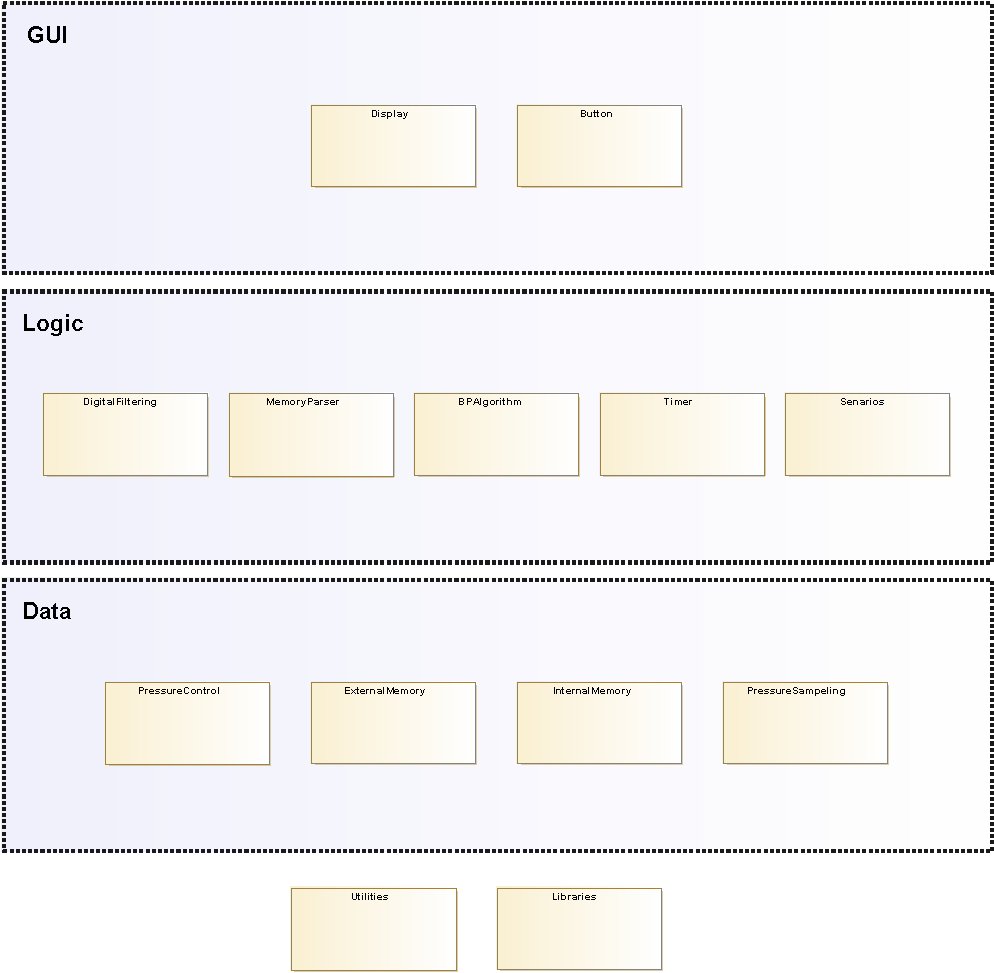
\includegraphics[width=\textwidth]{Implementeringsdokument/klassediagram_forsimplet-crop.pdf}
	\caption{Forsimplet klasse diagram}\label{fig:classDiagramSimple}
\end{figure}
\newpage

\input{Implementeringsdokument/filer/GUILaget}

\input{Implementeringsdokument/filer/LogikLaget}

\input{Implementeringsdokument/filer/DataLaget}

\input{Implementeringsdokument/filer/helpMetoder}
	
	\newpage
\section{Filter design} \label{title:filters}

\subsection{Analoge filtre}

Det analoge filter design har blandt andet funktionen at isolerer og forstærke DC niveauet fra tryksensoren, som er koblet til manchetten. Tryksensoren (MPX5100) er lineær og kan derfor ud fra en enkel koefficient kalibreres.1 DC niveauet skal forstærkes for at øge ADC opløsningen i forhold til mmHg per bit. Arduino MEGA 2560 har en ADC opløsning på 10bit. I volt er dette en opløsning på 5/1023=4.9mV. Sensoren har en sensitivitet på 45mV/kPA, svarende til 6mV/mmHg. Uden DC forstærkning er opløsningen altså 4.9/6=0.817mmHg. Ved at anvende gain X2 øges opløsningen til 0.817/2=0.408mmHg. Ren DC opnås ved at lavpas filteret fjerner alt AC over knækfrekvensen.

\begin{figure}[H]
	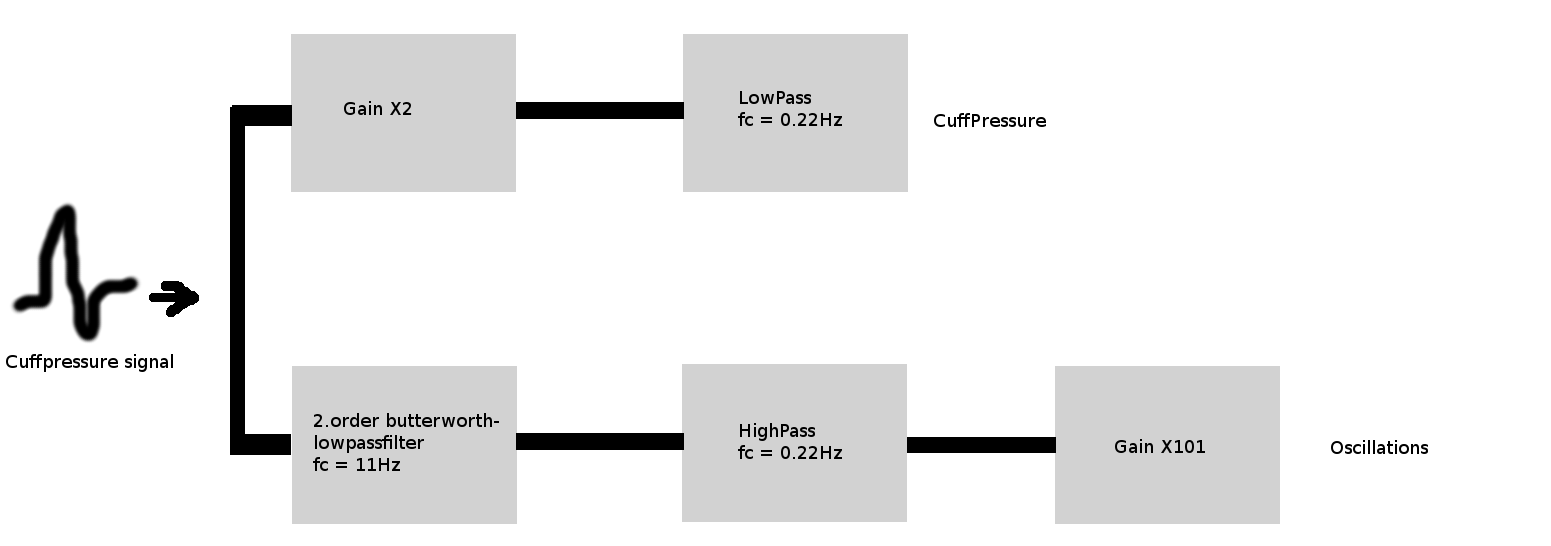
\includegraphics[width=\textwidth]{billeder/AnalogFilter.png}
	\caption{Filter model med inputsignal til venstre og de to output signaler	til højre}\label{pic:analogfilter}
\end{figure}
CuffPressure er forstærket DC og Oscillations er forstærket AC mellem 0.22Hz og 11Hz

Oscillationerne i manchetten isoleres med 11Hz anden ordens butterworth for at opnå god dæmpning på 50Hz brummen. L.A. Geddes et al. Sætter knæk frekvensen til 30Hz2, men efter som at puls signalet befinder sig på ca 1Hz og at Geddes med høj sandsynlighed har anvendt kaskade filtre sættes butterworth filterets knæk til 11Hz, svarende til elve afledte af puls grund frekvensen. Højpasfilteret fjerner DC ved at knække ved 0.22Hz. For at forstærke oscillationerne op i en størrelse, som arduinoen kan sample forstærkes det pulserende signal med gain X101.

\subsection{Komponent udregninger}
\input{filer/filterCalculations}

\subsection{Praksis}
Signal generator med frekvens 0.8Hz svarende til en sund puls. Simuleringen er vist på billederne under. Den lilla kurve er inputsignalet, rød er det oscillerende udgangssignal efter filteret og den grønne kurve er udgangssignalet efter det ikke oscillerende filter.

\begin{figure}[H]
	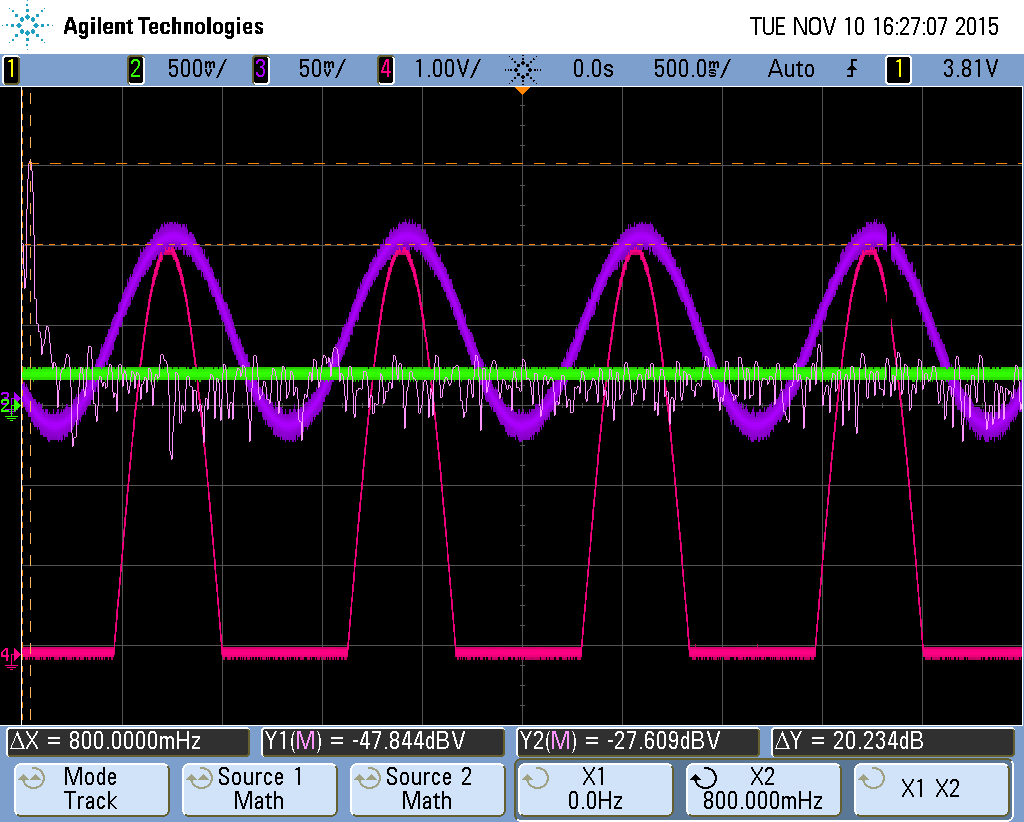
\includegraphics[width=\textwidth]{billeder/scope_9.png}
	\caption{Lilla er input sinus 0.8Hz. Grøn er ren DC. Rød er det filtrerede signal med oscillationerne. Den lyserøde kurve er FFT af det lella signal, hvor det ses at det består af 0.8Hz grundtone.}\label{fig:filterone}
\end{figure}

\begin{figure}[H]
	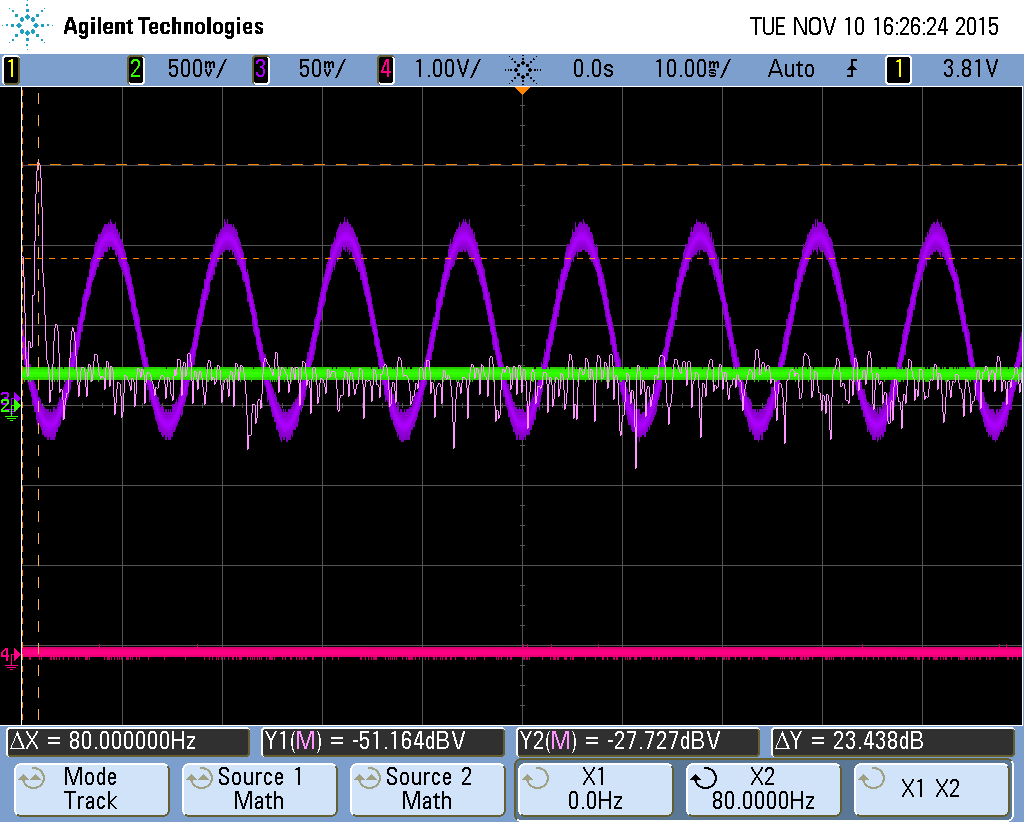
\includegraphics[width=\textwidth]{billeder/scope_8.png}
	\caption{Lilla er input sinus 80Hz. Grøn er ren DC. Rød er det 	filtrerede signal med oscillationerne. Den lyserøde kurve er FFT af det lella signal, hvor det ses at det består af 80Hz grundtone.}\label{fig:filtertwo}
\end{figure}
\newpage

\begin{figure}[H]
	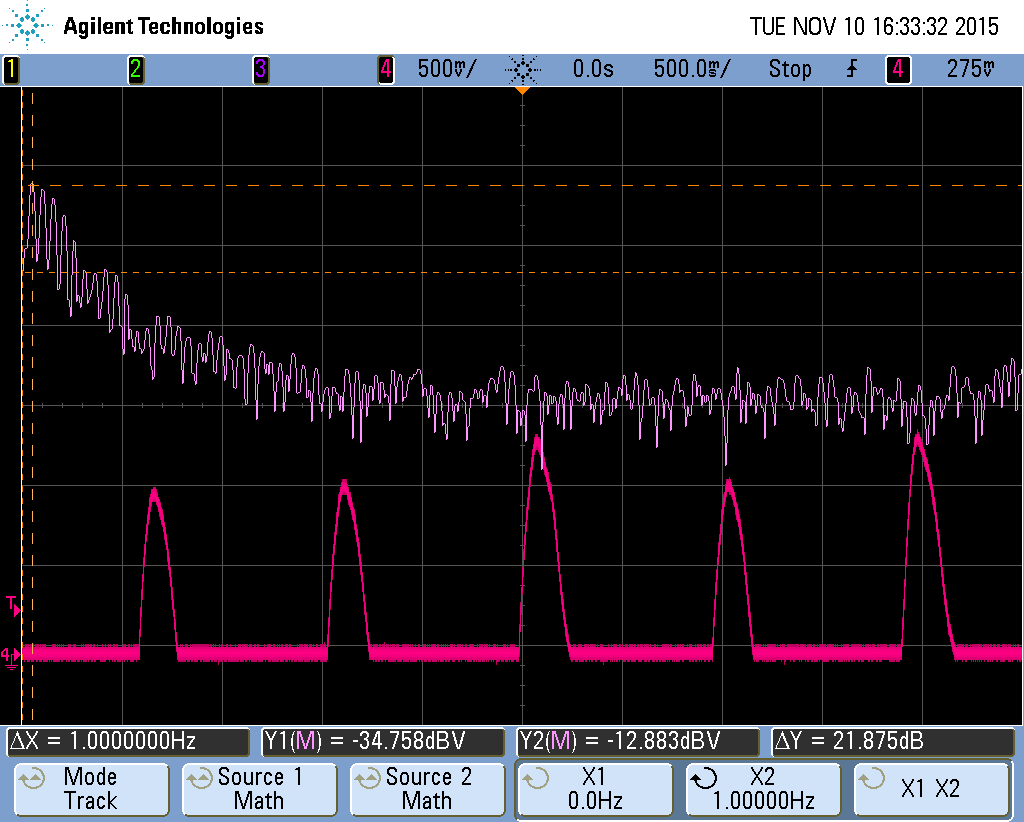
\includegraphics[width=\textwidth]{billeder/scope_10.png}
	\caption{Oscilloskop billedet viser udgangssignalet efter den oscillerende 	filtrering (Rød) og en FFT af signalet (lyserød). Her ses det tydeligt at grundtonen er ca 1Hz og har mindst 4 afledte der af 	(2,3,4,5 Hz), som gider den spidse smalle form.}\label{fig:filterthree}
\end{figure}

Hvis manchet signalet ikke simuleres, men i stedet måles på et rigtigt menneske ligner signalet ikke perfekte sinuser, men i stedet korte udsving, med en grundfrekvens og en masse overtoner. På nedenstående billede ses forskellige typiske udgangssignaler under en normal blodtryksmåling.
\newpage

\begin{figure}[H]
	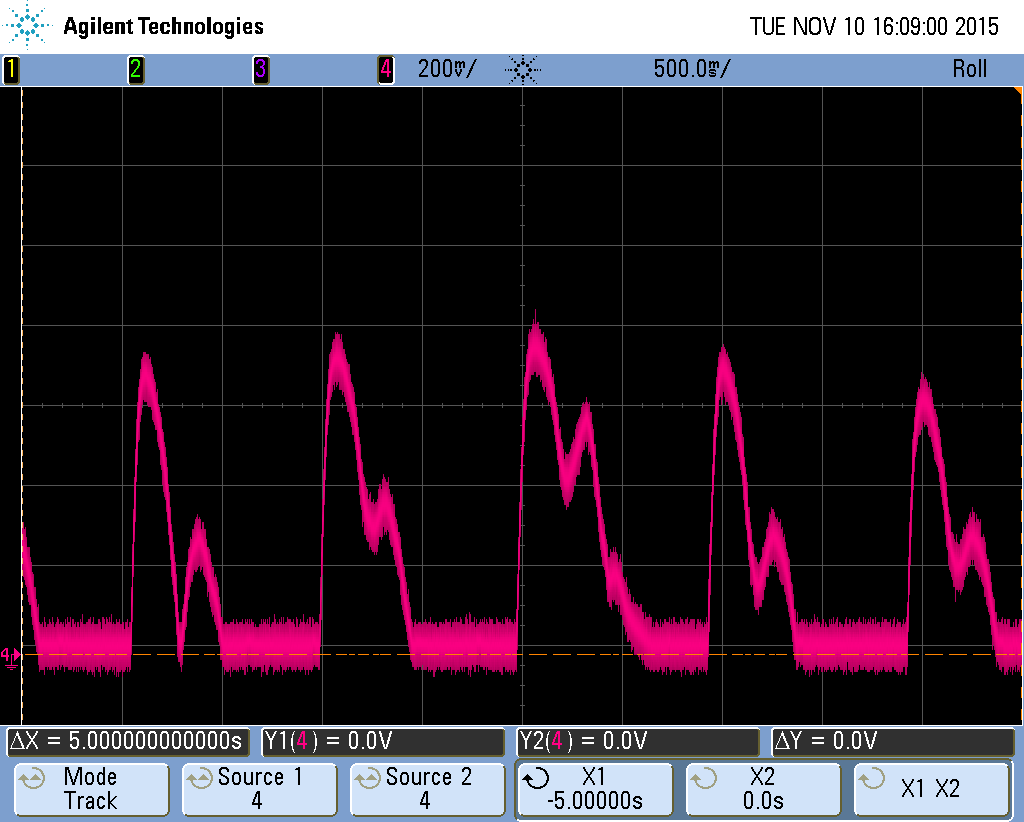
\includegraphics[width=\textwidth]{billeder/scope_2.png}
	\caption{Når manchet trykket nærmer sig det systolliske tryk obesrveres 	der et signal som ser lidt anderledes u.}\label{fig:filterfour}
\end{figure}

Det ses meget tydeligt på billede (se figur \ref{fig:filterthree} og \ref{fig:filterfour}) at det pulserende signal svinger meget med hensyn til peak amplituden over tid. Dette fænomen ses kan skyldes mange ting, her iblandt respirationen og andre mekaniske bevægelse. Den analoge filtrering når sin begrænsning, da den ikke kan filtrere peak amplituden til at passe en optimal blodtryksmåling, som kan ses på figur \ref{fig:goodMeasurement}, hvor amplituderne er konstant stigende ind til MAP og så aftagende efterfølgende. Til at håndterer dette problem anvendes der digital filtrering.
\newpage

\begin{figure}[H]
	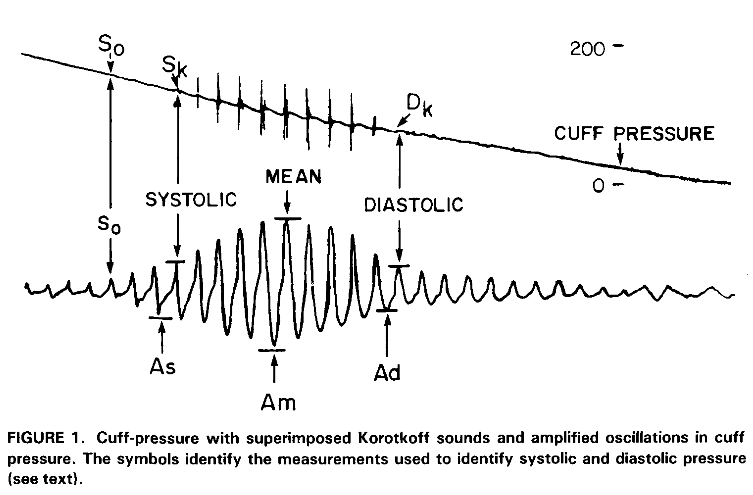
\includegraphics[width=\textwidth]{billeder/OptimalBlodtryksmaling.png}
	\caption{Signal fra oscillometrisk blodtryksmåling }\label{fig:goodMeasurement}
\end{figure}
Reference \fixme{Billedet er taget fra CHARACTERIZATION 	 OF THE OSClLLOMETRlC METHOD FOR MEASURING INDIRECT BLOOD 	PRESSURE}

\subsection{Digital filtrering}
Til digital filtrering er der anvendt et ekspotentiel midlingsfilter med zero group delay.
\begin{equation}
	y(n) = \alpha x(n)+(1-\alpha )y(n-1)
\end{equation}
Filteret midler peak ampletryderne, så den gennemsnitlige ampletyde forøgelse/dæmpning kommer til udtryk. Blodtryks filteret anvender en alfaværdi på $\alpha = 0.11$. Udermere filtreres data fra begge sider, altså først fra venstre mod højre og så bag efter fra højre mod venstre. Denne teknik sikre ingen group delay, som er vigtigt for at kunne bestemme MAP, som det tryk der er i manchetten på samme tidspunkt som den maksimal målte peak ampletyde. Dette er bedst ilistreret på figur XX, hvor manchettrykket er faldende over tid og peak amplituderne er stigende og efter MAP så faldende. Når det rå signal midles fra venstre mod højre opstår et group delay på peak ampletyderne, som ikke er på manchet tryk data'en. Af denne grund må der ikke være group delay på signalet.

\begin{figure}[H]
	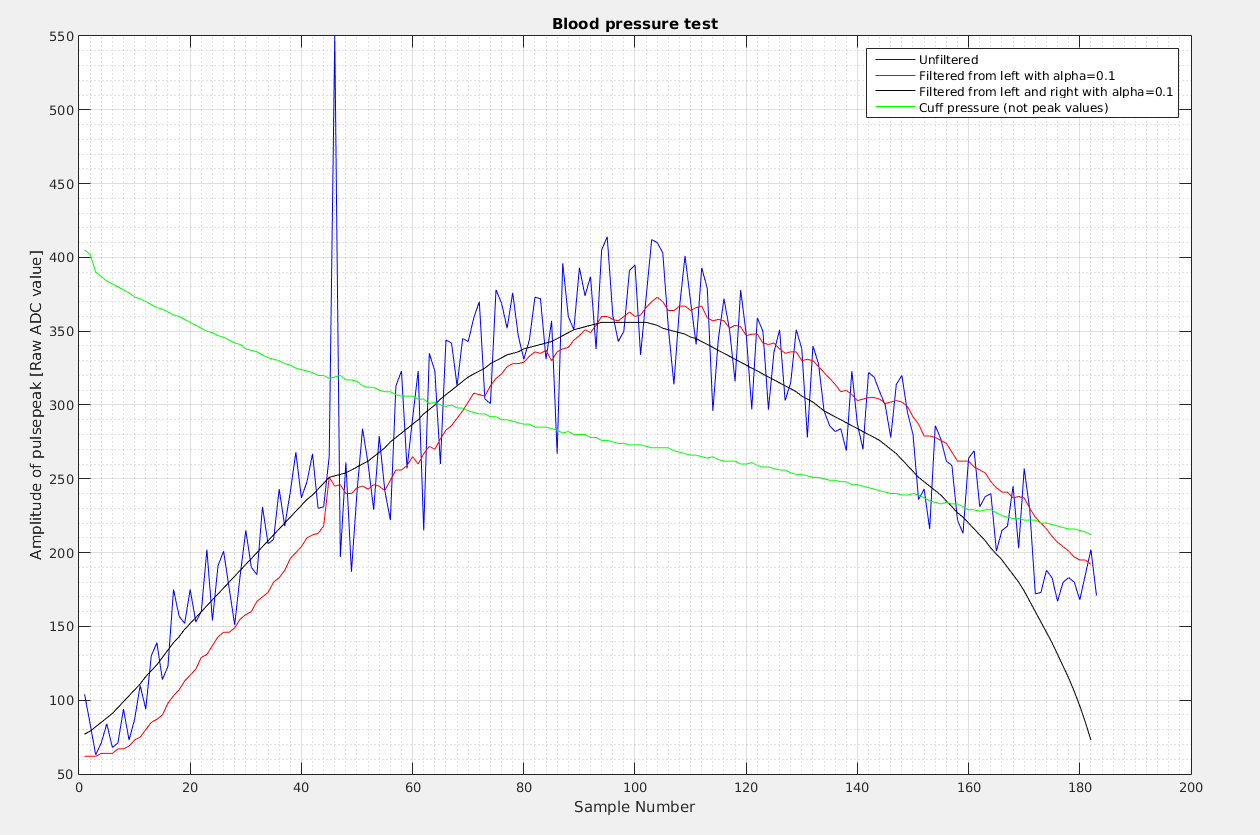
\includegraphics[width=\textwidth]{billeder/4_11_2016_udenMap.png}
	\caption{Graf med data fra en blodtryksmåling. Her ses at det rå signal 	er støjfyldt. Grøn er manchet trykket, blå er de rå peak amplituder, rød er filtreret en gang fra venstre mod højre, sort er filtreret fra begge sider 	}\label{fig:filterWithoutMap}
\end{figure}


	
	\newpage
\chapter{Hardware}

\section{Schmetic}
På figur \ref{fig:schematics} ses tegning over hardware setup. \textit{Signal in}, \textit{Signal out(A3)} og \textit{Signal out(A4)} skal ses som interface med arduino og tryksensoren. Disse er undladt for ikke gøre diagrammet for kompleks.
\begin{figure}[H]
	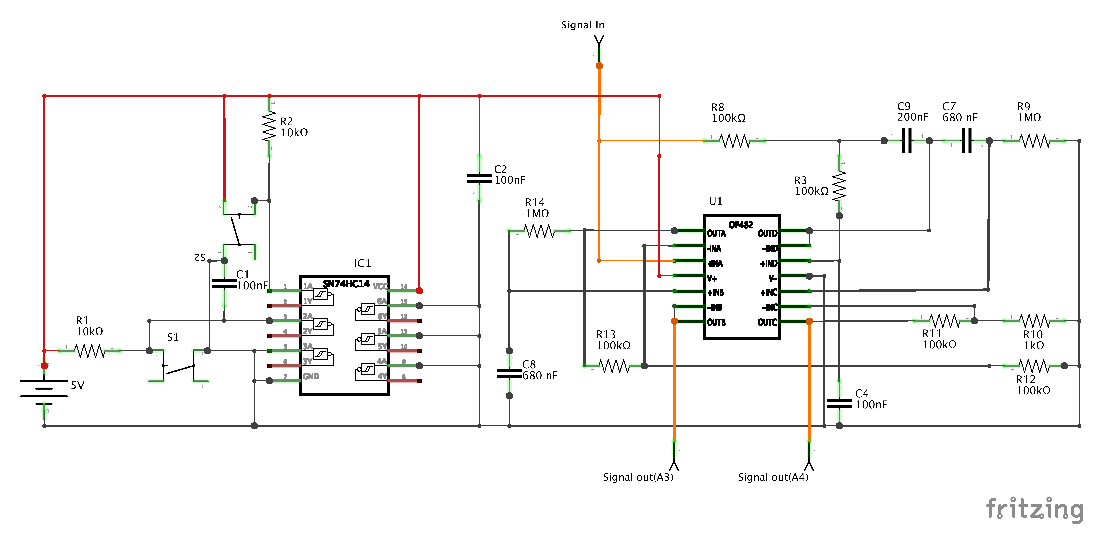
\includegraphics[trim = 0 30 0 0, clip=true, width = \textwidth]{Implementeringsdokument/billeder/Konditionering_schem.pdf}
	\caption{}\label{fig:schematics}
\end{figure}

\newpage
\section{Knapper} \label{title:buttons}
For at imødegå debouncing ved tryk på knapperne, er der bygget et støttekredsløbs til disse. Debouncing kan ses på figur \ref{fig:withbounce} hvor det mekaniske slip på knappen, giver anledning til en løs forbindelse ses på multimeteret som en lav efterfulgt af en høj, for så at blive lav igen. Microcontrolleren er hurtig nok til at registrer dette som et nyt knaptryk.
\begin{figure}[H]
	\begin{minipage}{0.50\textwidth}
		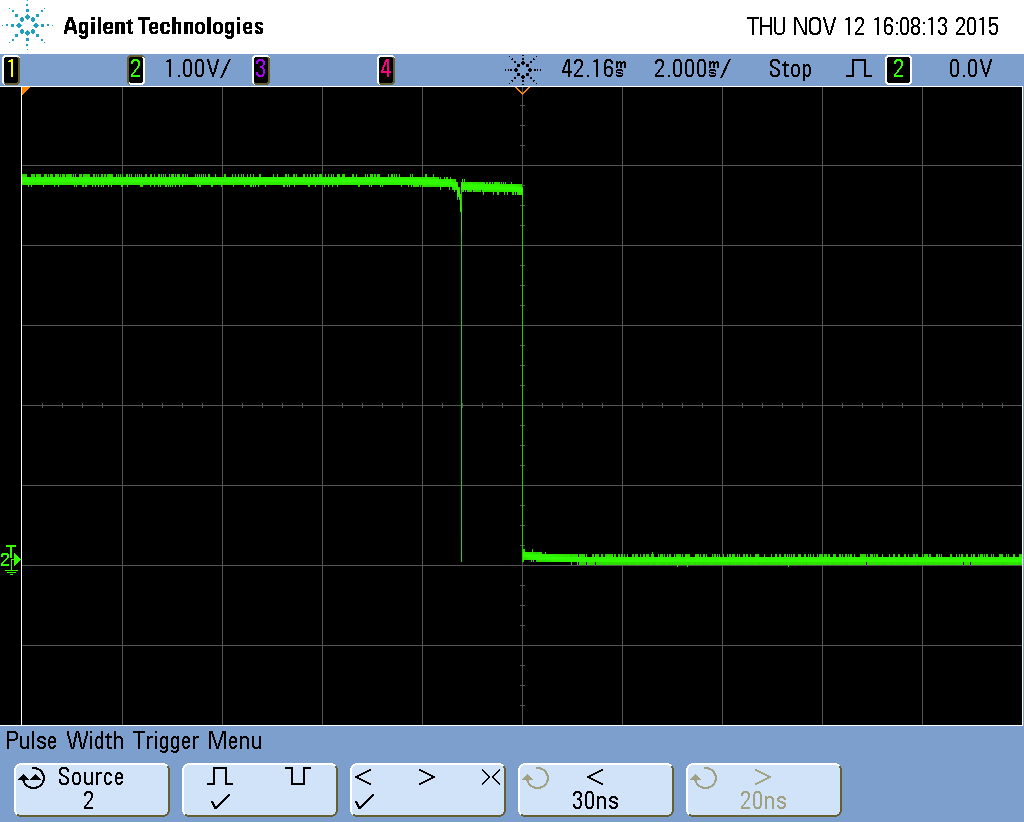
\includegraphics[width = \textwidth]{Implementeringsdokument/billeder/scope_14.png}
		\caption{Figuren viser et knaptryk, hvor der opstår debouncing.}\label{fig:withbounce}
	\end{minipage}
	\begin{minipage}{0.50\textwidth}
		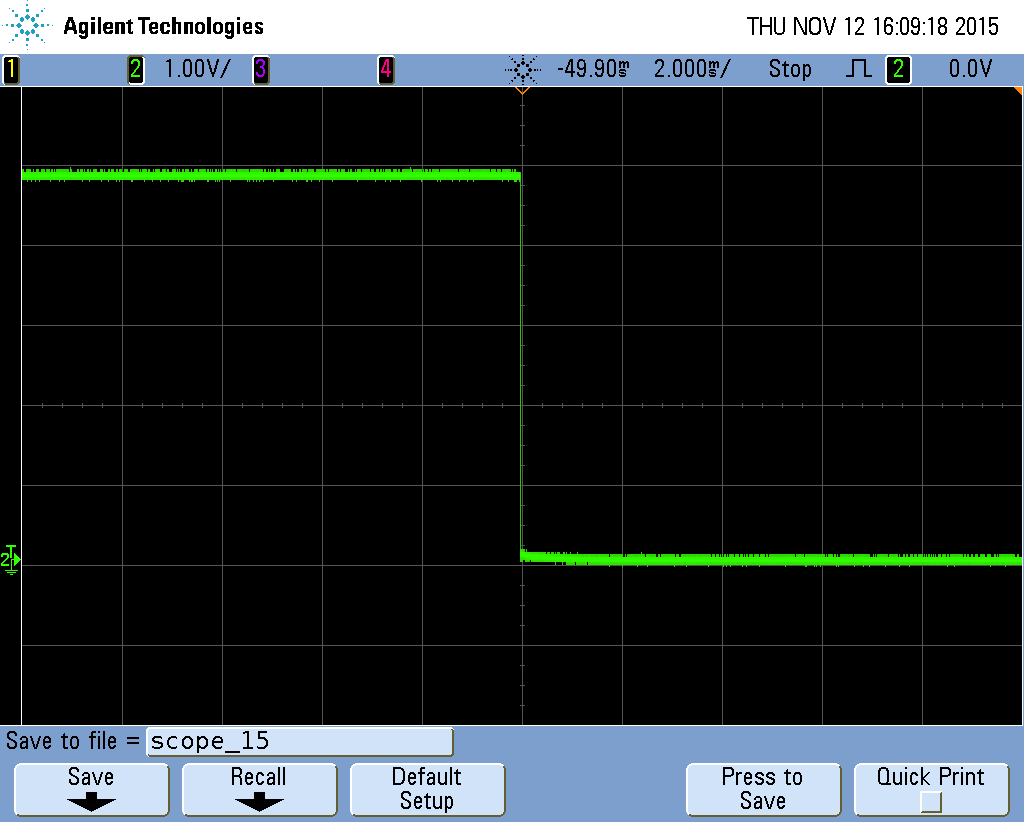
\includegraphics[width = \textwidth]{Implementeringsdokument/billeder/scope_15.png}
		\caption{Knaptryk hvor der er implementeret et anti debouncing kredsløb.}\label{fig:withoutbounce}
	\end{minipage}
\end{figure}

For at imødekomme  er der implementeret et debounce kredsløb (figur \ref{fig:antidebouncingcircuit}) med en inverting schmitt trigger. Schmitt triggeren leverer en stabil høj og kapacitoren forhindre den lav ved kortvarig open circuit under knaptryk. 
\begin{figure}[H]
	\centering
	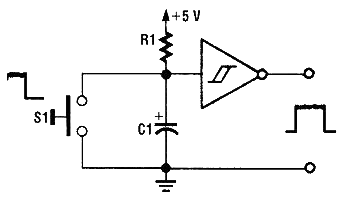
\includegraphics[width = 0.4\textwidth]{Implementeringsdokument/billeder/debounceSchematic.png}
	\caption{Anti debouncing kredsløb}\label{fig:antidebouncingcircuit}
\end{figure}

\section{Filter}
Filtreringen af signalet er opdelt i isolering af manchet tryk og isolering af pulserende signal. På figur \ref{fig:filterschematics} ses opdelingen af signalet i to til ADCen. Dyberer forklaring af filterdesignet kan findes under afsnit \ref{title:filters} omkring filter design.

\begin{figure}[H]
	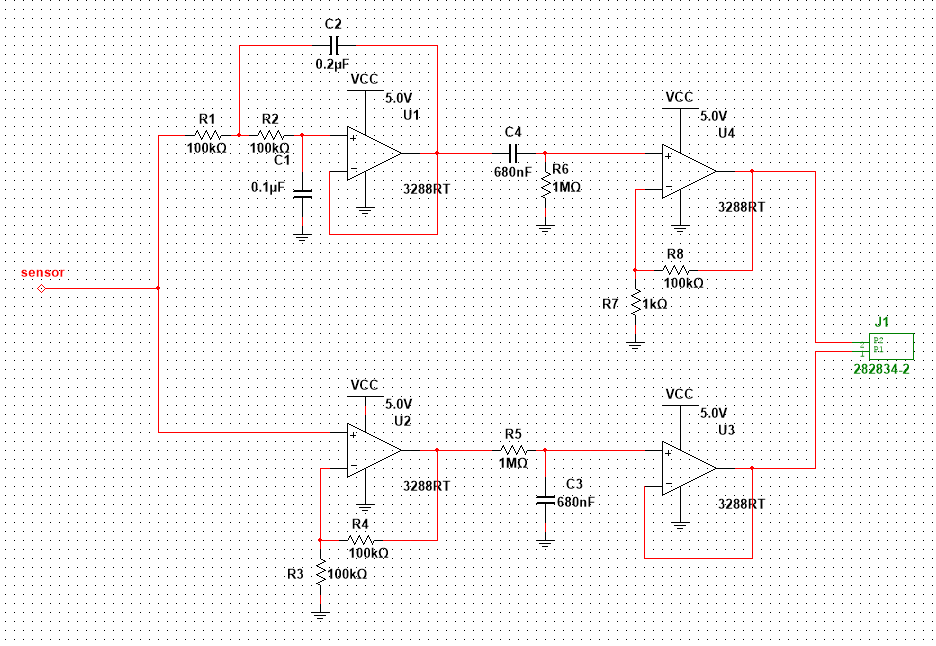
\includegraphics[width = \textwidth]{Implementeringsdokument/billeder/filterSchematics.PNG}
	\caption{Schematics over filter design}\label{fig:filterschematics}
\end{figure}

\section{Timer}
For at kunne lave tidsstempler til målinger med \textit{konditioneringsapparatet} var prototypen nød til at have en real time clock, som kunne holde korrekt tid, selvom apparatet blev slukket. Dette er opnået ved hjælp af en \textit{timekeeping chip} model DS1302 (Se datablad \cite{Manual:2}. Når prototypen er tændt forsynes den via \textit{konditioneringsapparatets} strømforsyning, og når prototypen er slukket forsynes DS1302 med et knapcelle batteri. Se figur \ref{fig:timerschematic} for at se hvordan timeren er komplet på arduino. 
\begin{figure}[H]
	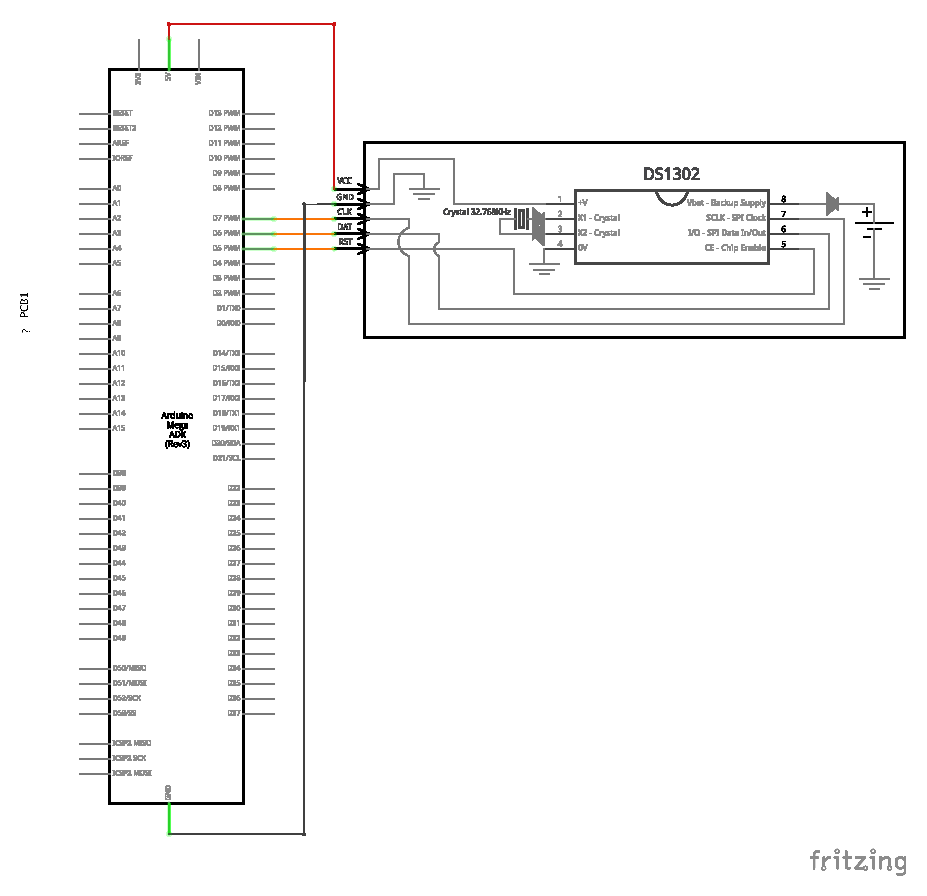
\includegraphics[trim = 15 30 0 0, clip = true, width = \textwidth]{Implementeringsdokument/billeder/Timer_schem.pdf}
	\caption{Oversigt over hvordan DS1302 er forbundet}\label{fig:timerschematic}
\end{figure}

\section{Display}
Til styring af bruger interfacet og feedback. Displayet er 2.2" med en opløsning på 320x240. Displayet styres med IC'en ILI9340 (Se datablad \cite{RefWorks:14}). Kommunikation med displayet foregår via en SPI forbindelse som er koblet til Arduino Mega's digitale port 50, 51 og 52. For komplet interface se figur
\begin{figure}[H]
	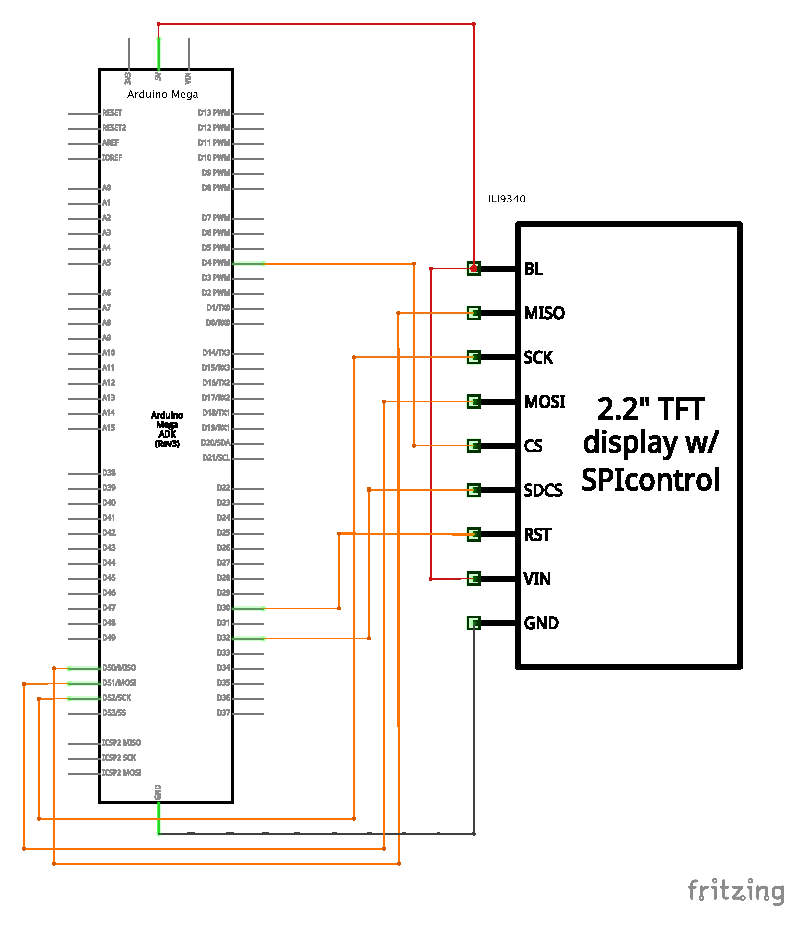
\includegraphics[trim = 10 30 0 0, clip = true, width = \textwidth]{Implementeringsdokument/billeder/Display_schem.pdf}
	\caption{Oversigt over hvordan ILI9340 er forbundet}\label{fig:displayschematic}
\end{figure}


\section{Motor shield}
Arduino motor shield implementerer L298P (se figur \ref{fig:shieldfront} og \ref{fig:shieldback} med selvinduktion beskyttelse og en adskillelse af motor forsyning og den logiske strømforsyning. Schematics over boarded er taget fra (\cite{Manual:3}). Desuden er motor shield modificeret, så det har en ekstern strøm forsyning på 12V. Derfor er 5V forbindelse mellem arduino og motor shield brudt.
\begin{figure}[H]
	\begin{minipage}{0.5\textwidth}
		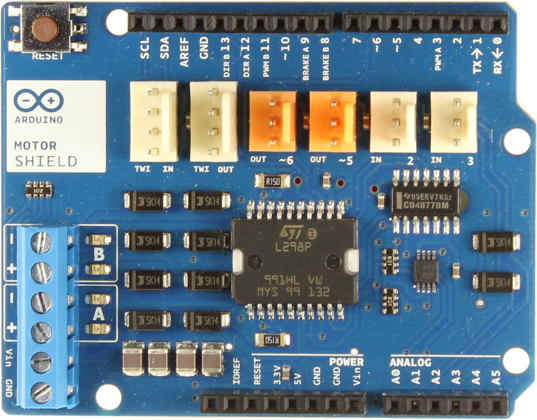
\includegraphics[width = \textwidth]{Implementeringsdokument/billeder/shieldforside.png}
		\caption{Arduino motorshield forside}\label{fig:shieldfront}
	\end{minipage}
	\begin{minipage}{0.5\textwidth}
		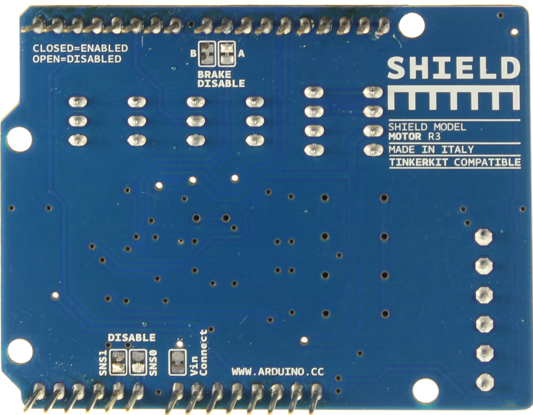
\includegraphics[width = \textwidth]{Implementeringsdokument/billeder/shieldbagside.png}
		\caption{Knaptryk hvor der er implementeret et anti debouncing kredsløb.}\label{fig:shieldback}
	\end{minipage}
\end{figure}

\label{lastPage}
	
\end{document}
\stopcontents[id]
\resumecontents[overall]

%%%% Kilder %%%%

\begingroup
\raggedright
\bibliography{bibtex/litteratur}							% Litteraturlisten inkluderes
\endgroup


%%%% Fixme-listen %%%%

\newpage														% Ny side til Fixme-listen
\listoffixmes													% Fixme-listen - fjernes til sidst i projektet med "%"



\end{document}


\stopcontents[overall]
\chapter{Resultater}

\section{Konditioneringsapparat}
Konditioneringsapparatet er opbygget af flere blokke, som kan ses på figur \ref{fig:BDD(SystemOverview)}. Blok Definition diagrammer beskriver relationerne mellem blokke, så som sammenhæng, forening og specialisering. I denne sammenhæng beskriver figur \ref{fig:BDD(SystemOverview)} opbygningen af konditioneringsapparatet. 
\begin{figure}[H]
	\centering
	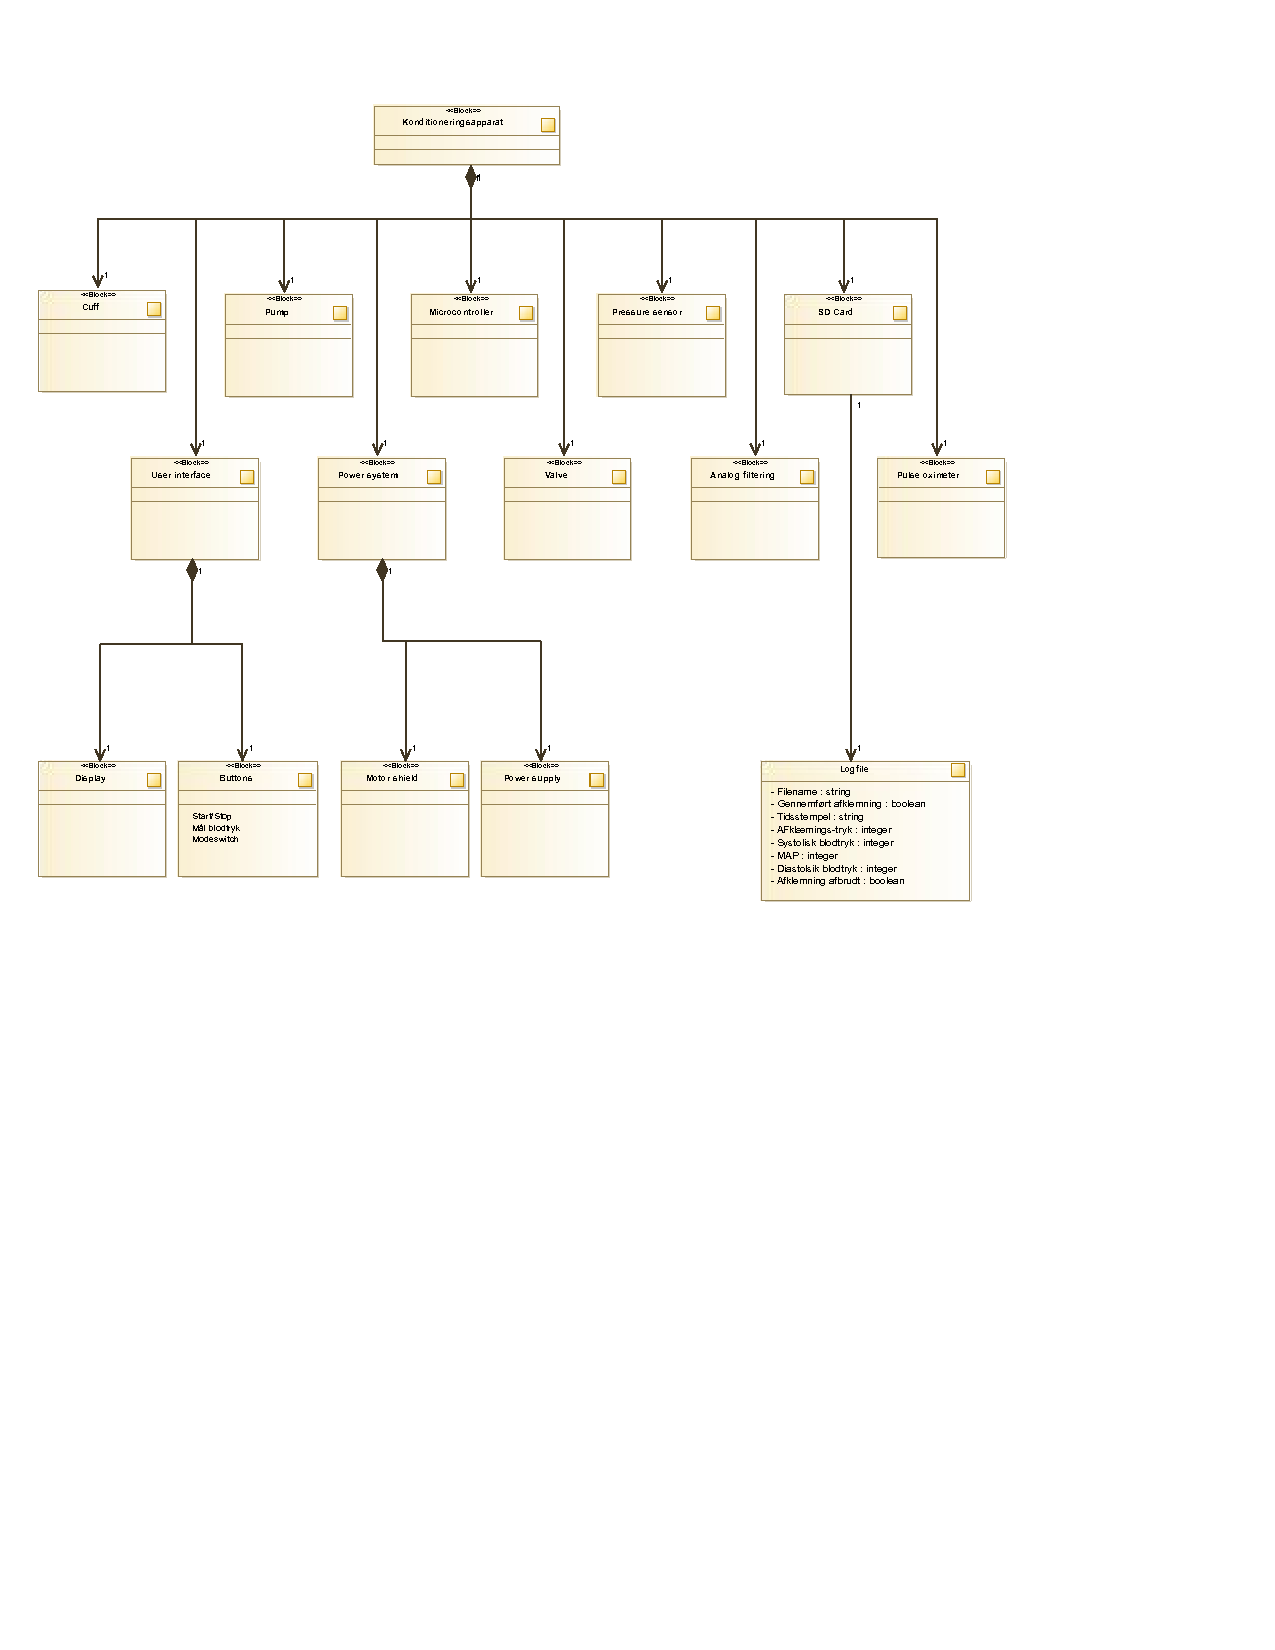
\includegraphics[width=0.9\textwidth]{billeder/BDD(SystemOverview).pdf}
	\caption{Block difinition diagram over konditioneringsapparatet.}\label{fig:BDD(SystemOverview)}
\end{figure}

\subsection{Oscilumetrisk blodtryks apparat}
Den oscillometriske blodtryks måle metode, beskrevet i afsnit \ref{noninvasivBloodpressureMeasurement}, er implementeret i implementeringsdokumentet\fixme{reff: implementeringsdokument} og resultaterne er beskrevet i dette afsnit.

Det pulserende signal fra tryksensoren, som blodtryksmåleren analyserer er i sin rå (ubehandlet) tilstand støjfyldt. Signalet beskrevet i afsnit \ref{noninvasivBloodpressureMeasurement} på figur \ref{fig:OscillometriskMetode} er meget rent og amplitudehøjderne danner en flot parabel formet kurve. På figur \ref{fig:rawPulseSignal} ses det pulserende signal direkte fra tryksensoren, som er indhyldet i støj. Kurven er stødt faldende, fordi trykket i manchetten langsomt lukkes ud. Ydermere observeres der også varierende amplitudehøjder, som ikke er stødt stigende/faldende, men virker som tilfældigheder.  

\begin{figure}[H]
	\centering
	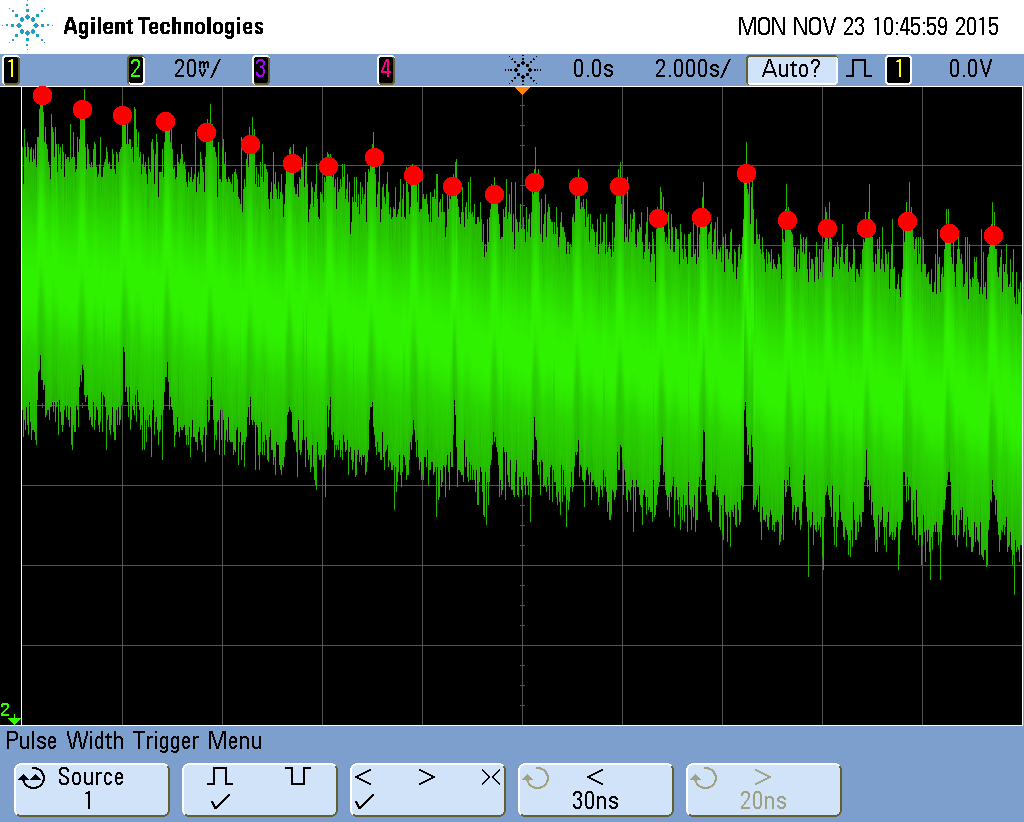
\includegraphics[trim={0 7cm 0 1.5cm},clip, width=1\textwidth]{billeder/rawPulseSignalPeaks.png}
	\caption{Oscilloskops måling af rå signal fra blodtryksmåling, med konditioneringsapparatet. De røde cirkler er pulse oscillationernes højeste punkt}\label{fig:rawPulseSignal}
\end{figure}

Efter analog filtrering af det rå signal på endnu en blodtryksmåling med konditioneringsapparatet, ses at amplitude oscillationerne isoleret og uden manchettrykket (offset). Over en hel blodtryksmåling skal kurven ifølge teorien (se figur \ref{fig:OscillometriskMetode}), starte med en stigende amplitude højde efterfulgt af en top og til sidst faldende oscillationshøjder med laverer hældnings koefficient end starten. En hel blodtryksmåling med filtreret råsignal kan ses på figur \ref{fig:filteredPulseSignal}.

\begin{figure}[H]
	\centering
	\subbottom[Stigende]{%
		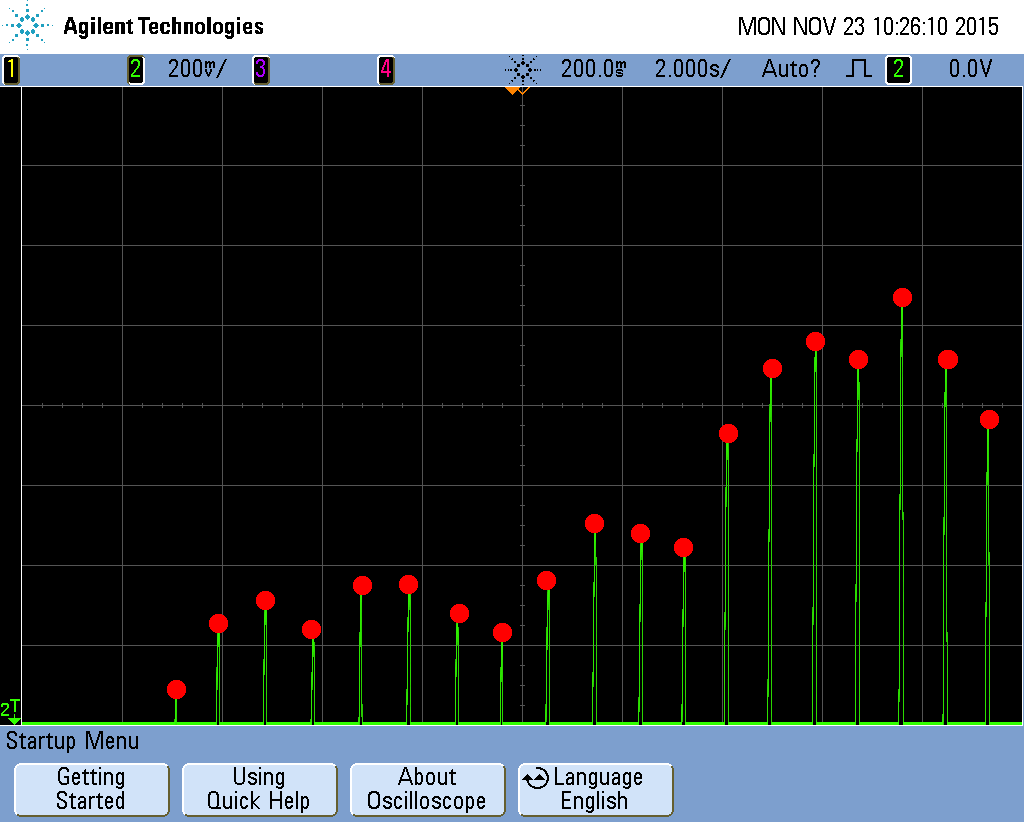
\includegraphics[trim={0 3.3cm 0 1.5cm},clip, width=0.328\textwidth]{billeder/filteredPulseSignalPeaks1.png}}
	\subbottom[Højdepunkt]{%
		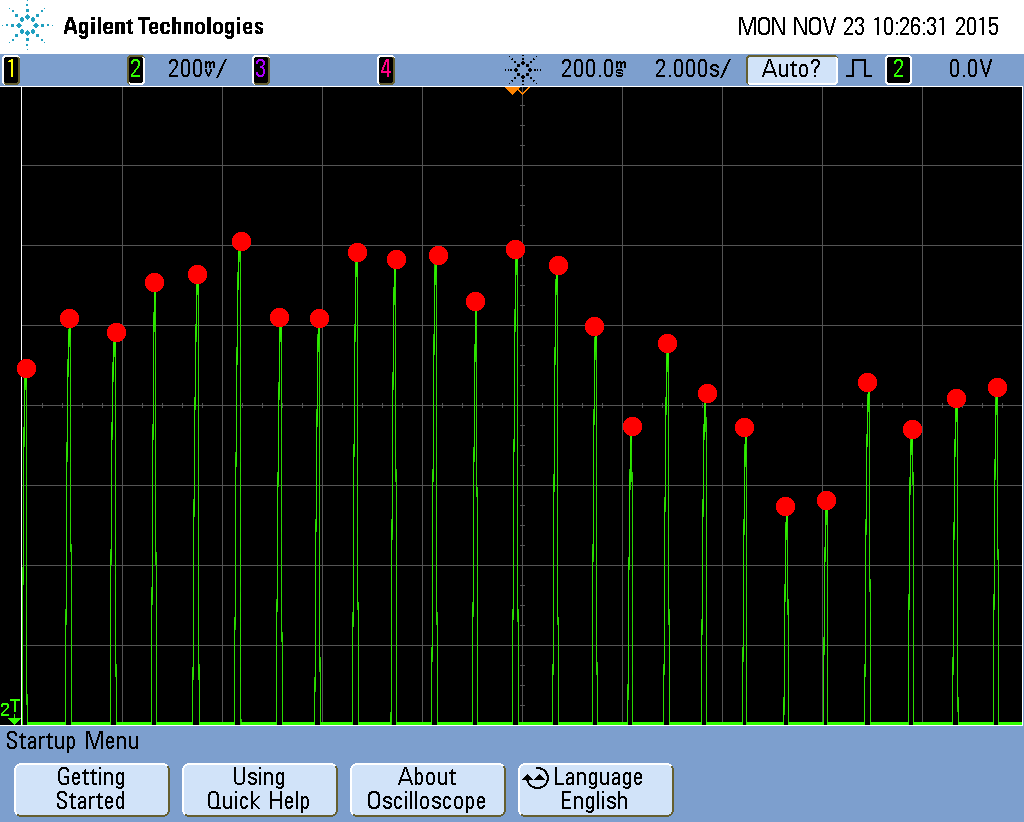
\includegraphics[trim={0 3.3cm 0 1.5cm},clip, width=0.328\textwidth]{billeder/filteredPulseSignalPeaks2.png}}
	\subbottom[Faldende]{%
		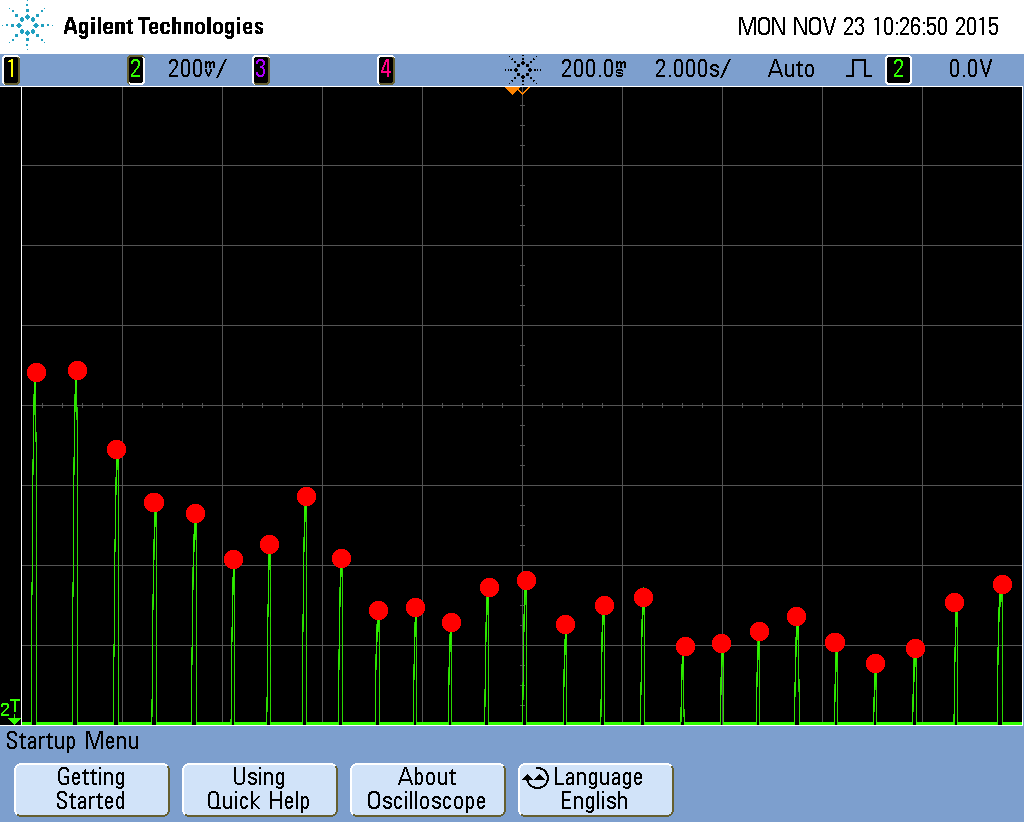
\includegraphics[trim={0 3.3cm 0 1.5cm},clip, width=0.328\textwidth]{billeder/filteredPulseSignalPeaks3.png}}
	\caption{Osclilloskops måling af filtreret signal af blodtryksmåling, med konditioneringsapparatet. (a) er første del af blodtryksmålingen, (b) er de midten af signalet med, hvor MAP befinder sig og (c) er slutningen af signalet, hvor amplituderne flader ud. De røde cirkler er pulse oscillotionernes højeste punkt}\label{fig:filteredPulseSignal}
\end{figure}

\subsubsection{Analog filtrering}
Den analoge filtrering, ses på forskellen mellem figur \ref{fig:rawPulseSignal} og figur \ref{fig:filteredPulseSignal}, er implementeret i implementeringsdokumentet se \fixme{ref: implementeringsdokument}. 
Det resulterende analoge filter, er bestemt ud fra test opsætninger (se \fixme{ref: implementeringsdokument}) og litteraturen \fixme{CHARACTERIZATION OF THE OSClLLOMETRlC METHOD FOR MEASURING INDIRECT BLOOD PRESSURE}. De pulserende oscillationer isoleret fra det rå signal kan ses på figur \ref{fig:filteredPulseSignalWithFFT}. Resultatet er opnået, ved at implementere et båndpasfilter, med et pasbånd som starter før lavest mulige puls\fixme{fortæl hvad det er} og slutter ved den tiende afledte af grundfrekvensen 60bmp (se figur \ref*{fig:BandPassFilter}).

\begin{figure}[H]
	\centering
	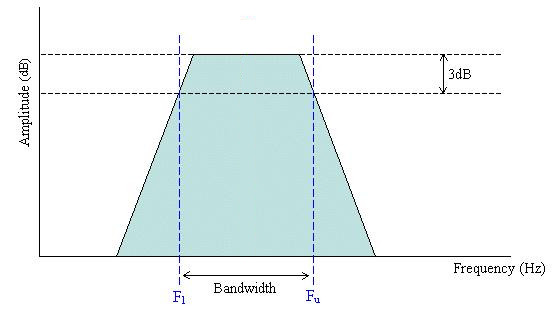
\includegraphics[trim={0 0 0 1.5cm},clip, width=0.8\textwidth]{billeder/BandPass_filter.JPG}
	\caption{Bånd pass filter med passfilter mellem $F_1$ og $F_u$. $F_1=0.22Hz$ (13 bmp under mulig puls) og $F_u=11Hz$ (660 bmp 10 afledte af 60 bpm) }\label{fig:BandPassFilter}
\end{figure}

\begin{figure}[H]
	\centering
	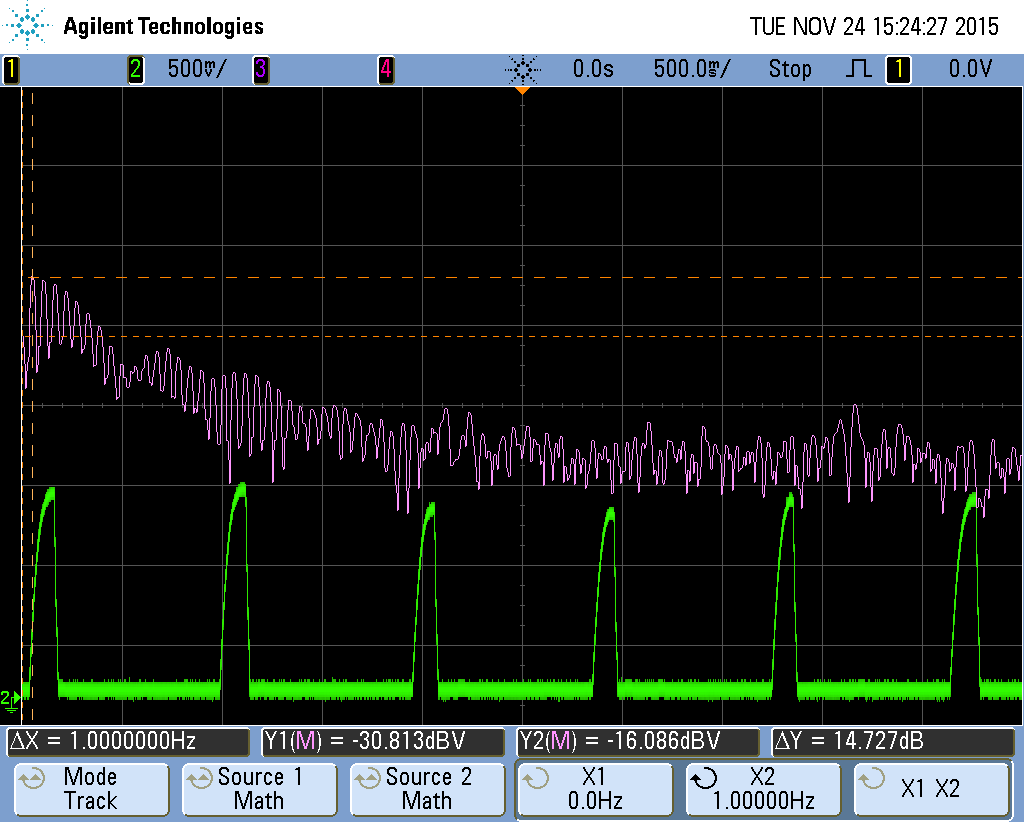
\includegraphics[trim={0 2.5cm 0 1.5cm},clip, width=0.8\textwidth]{billeder/filteredPulseSignalWithFFT.png}
	\caption{Osclilloskops måling af filtreret signal fra manchetten oppustet på arm. Den grønne kurve er de pulserende oscillotioner og den lilla kurve er en Fast Fourier Transformation (FFT) af den grønne kurve, hvor den udregnede grundfrekvens af oscillationerne måles til 1Hz (60 bpm).}\label{fig:filteredPulseSignalWithFFT}
\end{figure}

\subsubsection{Digital filtrering}
For at opnå en glat parabel, som vist på  figur \ref{fig:OscillometriskMetode}, er der implementeret et digitalt filter, som har til opgave at udglatte oscillutions amplituderne fra blodtryksmålingerne. Resultatet af implementeringen kan ses på figur \ref{fig:digitalFilterData}. Det bedste forhold mellem udglatning og reaktionshastighed af filteret er opnået ved et ekspotentielt midlingsfilter (se \ref{eq:ekspotentielmidlingsfilter}) med alfa værdi på 0.15 (se \fixme{reff: implementeringsdokument} for uddybende beskrivelse).  

\begin{equation}
y(n)=\alpha*x(n)+(1-\alpha)*y(n-1)
\label{eq:ekspotentielmidlingsfilter}
\end{equation}
\begin{figure}[H]
	\centering
	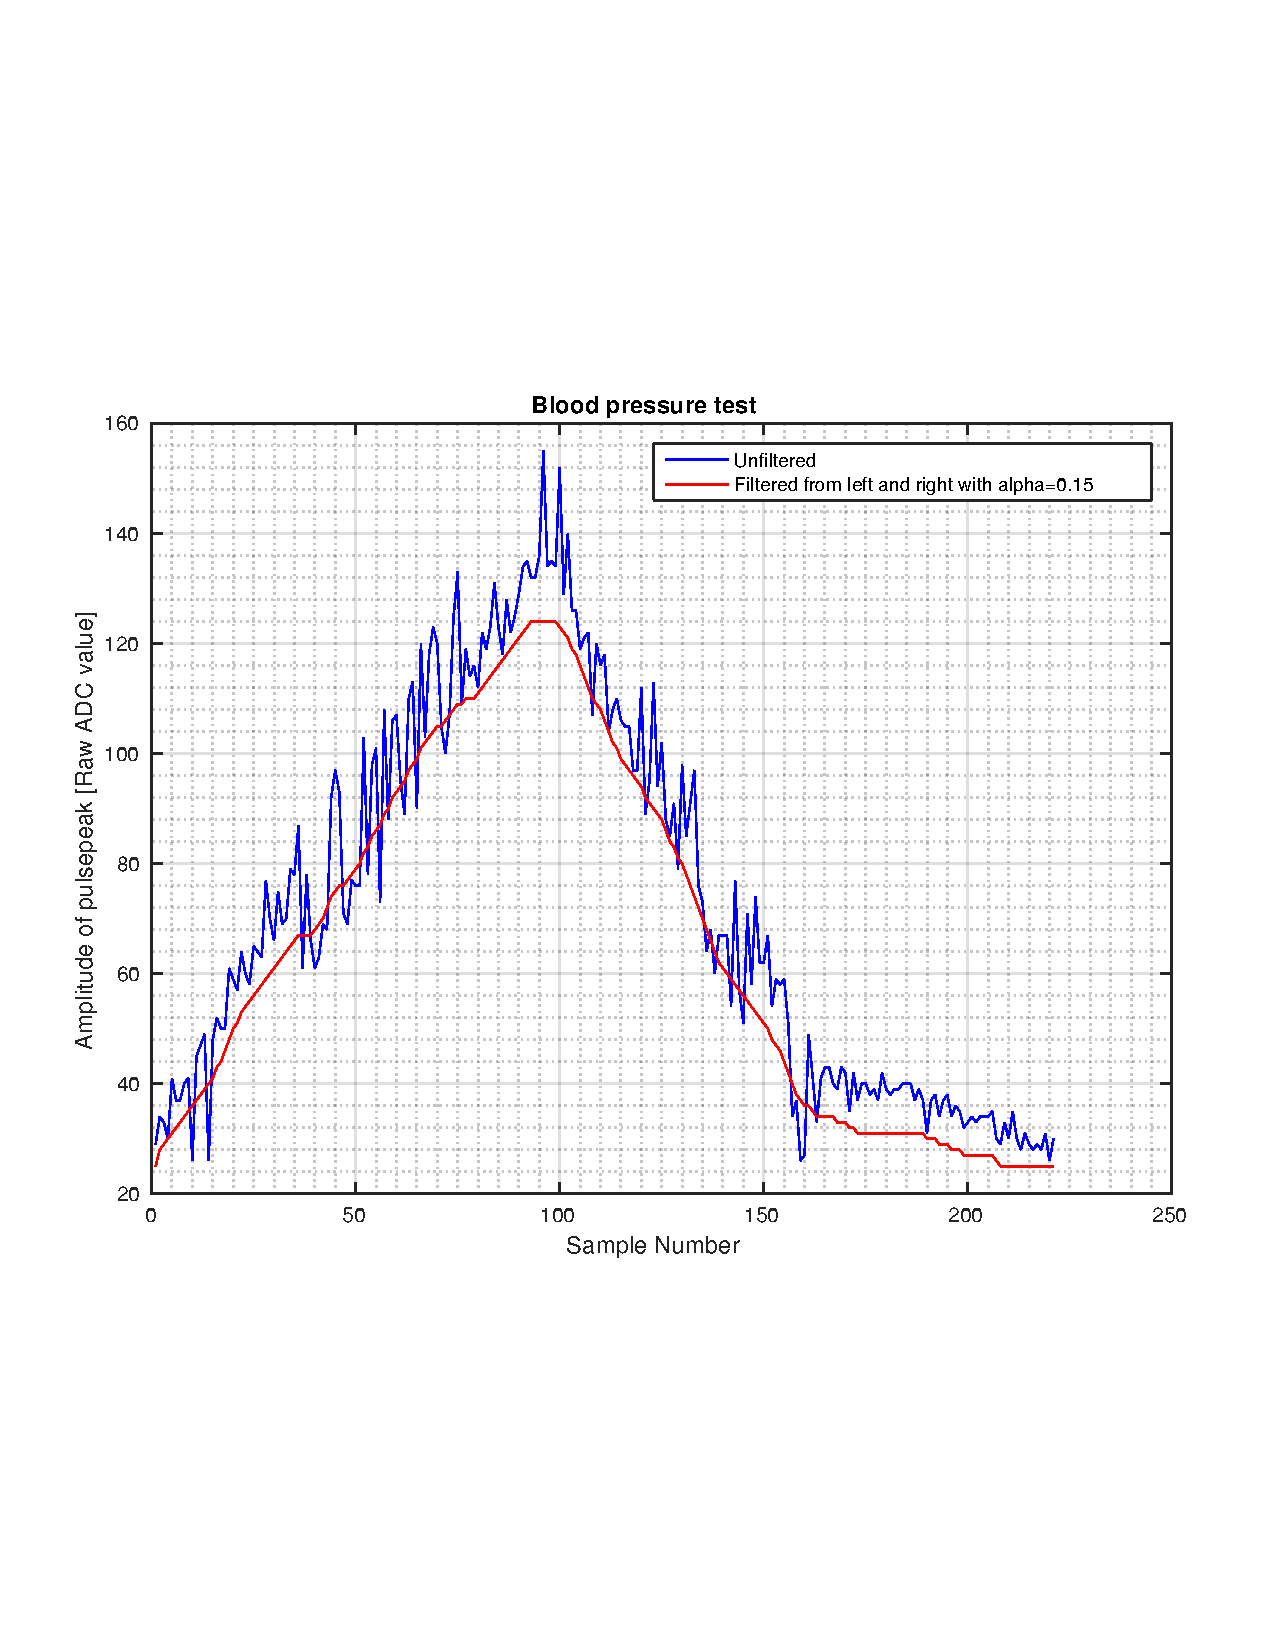
\includegraphics[trim={0 0 0 0},clip, width=0.7\textwidth]{billeder/digitalFilterData.pdf}	
	\parbox{10.5cm}{\caption{Digital filtrering af oscillotions peaks fra blodtryksmåling på simulator med ekspotentiel midlingsfilter.}\label{fig:digitalFilterData}}
\end{figure}


\subsection{Fikseret-ratio} \label{Fikseret-ratio}
Konditioneringsapparatets mest avancerede egenskab er uden tvivl estimering af blodtrykket. Apparatet anvender den oscillometriske metode hvor det systoliske og diastoliske tryk blandt andet bestemmes ud fra MAP. Under udviklingen af konditioneringsapparatet blev det besluttet at anvende den fikserede-ratio metode for at forsimple udviklingsarbejdet.

Fikseret-ratio metoden anvender empirisk data til at bestemme hvor store oscillationerne i manchettenv skal være i forhold til oscillationerne ved MAP, for at identificerer SYS og DIA. Dette betyder at systolisk og diastolisk tryk er bestemt ved manchettrykket når amplituden af oscillationerne er en ratio af den maksimale værdi.\fixme{ref: Theory of the Oscillometric Maximum and the Systolic and Diastolic Detection Ratios}

\begin{minipage}[c]{0.5\textwidth}
	Ratio værdierne til \textit{konditioneringsapparatet} kunne ikke bestemmes ud fra en større mængde empirisk data fra patienter, på grund af projektets omfang. I stedet er empirisk data blevet indsamlet fra "Fluke biomedicalBP Pump 2" en oscillometrisk blodtrykssimulator (se figur \ref{fig:TheFlukeBiomedicalBPPump2L}). \textit{Konditioneringsapparatet} opsamlede data fra simulatoren, hvilket kan ses på figur \ref{fig:digitalFilterData} og \ref{fig:digitalFilterDataSysMapDia}. Fordi simulatoren indstilles til kendte blodtryksværdier kan de fikserede-ratiorer bestemmes ud fra oscillations amplituden (OA) ved et givent manchettryk. f.eks ved simulering af 120/80 skal oscillations amplituden ved manchettrykket 120mmHg aflæses og forholdet mellem MAP og denne aflæste værdi er den systoliske ratio.
	
	
\end{minipage}
\begin{minipage}[c]{0.5\textwidth}
	\begin{figure}[H]
		\centering
		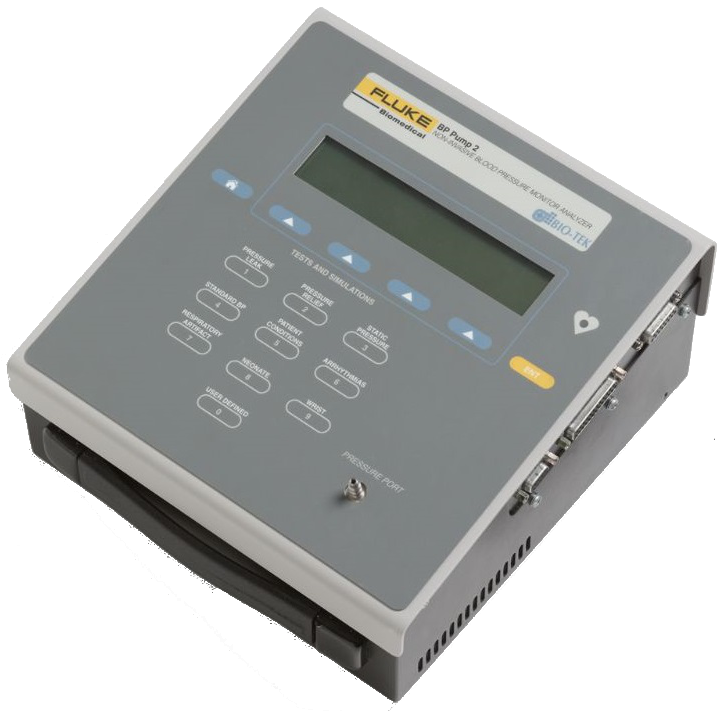
\includegraphics[trim={0 0 0 0},clip, width=0.9\textwidth]{billeder/TheFlukeBiomedicalBPPump2L.png}	
		\parbox{7cm}{\caption{Fluke Biomedical BP Pump 2 Non-invasiv blodtrykssimulator}\label{fig:TheFlukeBiomedicalBPPump2L}}
	\end{figure}
\end{minipage}

Resultatet af simulationerne kan ses på figur \ref{fig:digitalFilterDataSysMapDia1} uden manchettrykket og med manchettrykket på figur \ref{fig:digitalFilterDataSysMapDia2}. Ratioen for SYS (se \ref{eq:sysratio}) blev udregnet til 0.38 og for DIA (se \ref{eq:sysratio}) til 0.48. 
	\begin{equation}
	SYS_{OA}=MAP_{OA}*0.38
	\label{eq:sysratio}
	\end{equation}
	\begin{equation}
	DIA_{OA}=MAP_{OA}*0.48
	\label{eq:diaratio}
	\end{equation}

\begin{figure}[H]
	\centering
	\subbottom[Simulationsdata uden manchettryk]{\label{fig:digitalFilterDataSysMapDia1}%
		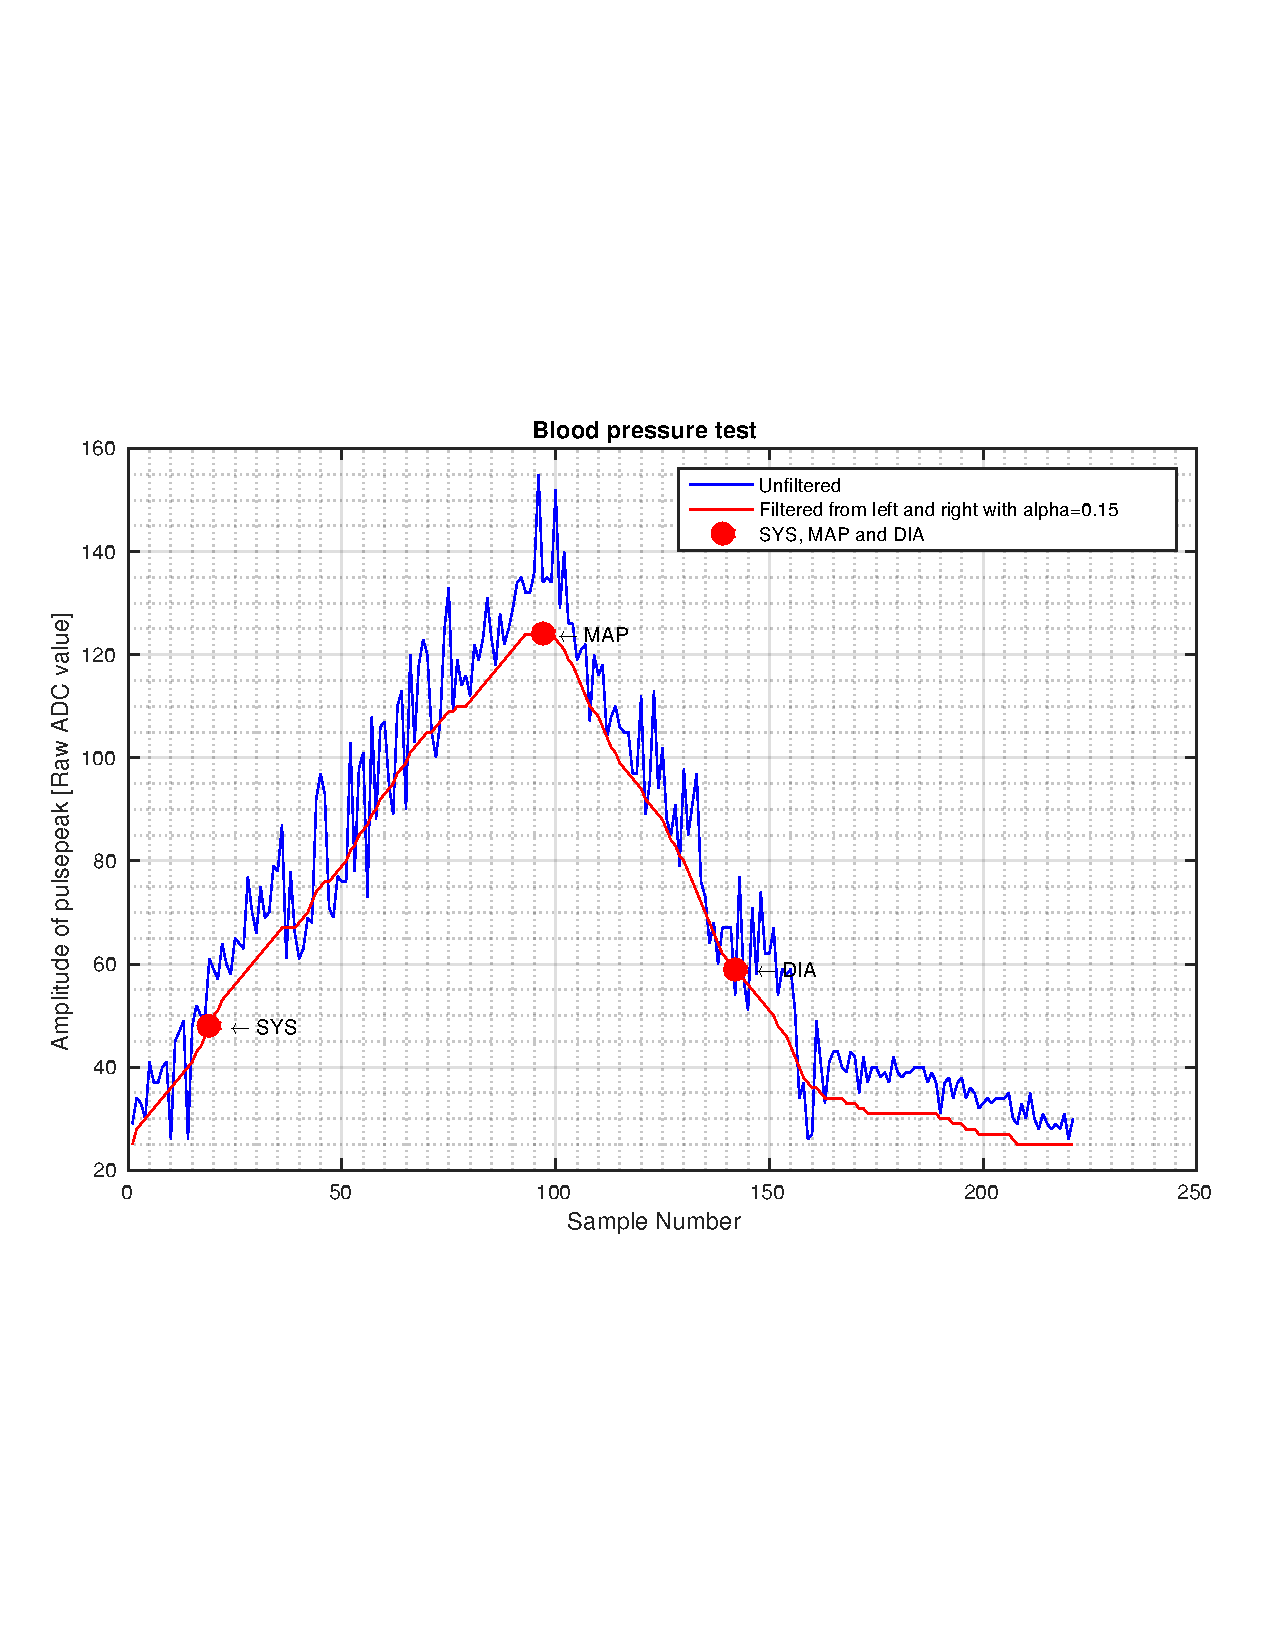
\includegraphics[trim={0 0 0 0},clip, width=0.48\textwidth]{billeder/digitalFilterDataSysMapDia.pdf}}
	\subbottom[Simulationsdata med manchettryk]{\label{fig:digitalFilterDataSysMapDia2}%
		\includegraphics[trim={0 0 0 0},clip, width=0.48\textwidth]{billeder/digitalFilterDataCuffSysMapDia.pdf}}
	\caption{Digital filtrering af oscillotions amplituderne fra blodtryksmåling på simulator med ekspotentiel midlingsfilter. De røde prikker er placeret  hvor SYS, MAP og DIA befinder sig ved fikseret-ratio på 0.38(SYS) og 0.48(DIA).}
\end{figure}
  

\section{Dataopsamling}
I forbindelse med udviklingen af prototypen var der et ønske fra kunden side omkring dataopsamling fra \textit{Konditioneringsapparatet}. For at apparatet kan bruges til forskningsprojektet er nødvendigt, at kunne dokumentere hvor mange konditioneringscyklusser en patient har modtaget. I samarbejde med kunden blev aftalt at et \textit{konditioneringsapparat} skal følge en patient i gennem hele forløbet, altså fra præhospital, til hospital og til sidst i hjemmet. Derfor blev det besluttet at data blev gemt på et SD kort, som hver gang et apparat returneres fra en patient bliver tømt for data og formateret. 

\begin{figure}[H]
	\includegraphics[width = \textwidth]{billeder/fileksempel-crop.pdf}
	\caption{Et eksempel på fil udtræk fra SD kortet}\label{fig:fileksempel}
\end{figure}

På figur \ref{fig:fileksempel} oversigt over fil udtræk. Her er udført en konditioneringsbehandling, hvor blodtrykket først er blevet målt til 174/100(124) mmHg. Der gemmes en værdi ved blodtryksmåling, hver gang trykket i manchetten når afklemningstrykket og når en okklusionsfase er færdig. Endvidere skrives det til SD kortet hvis konditioneringsbehandlingen afbrydes. Hver gang der skrives til SD kortet gemmes et tidsstempel, om afklemningen er gennemført, afklemningstrykket, blodtrykket og information omkring konditioneringsbehandling blev færdig gjort. 

I den måling der er vist på figur \ref{fig:fileksempel} er der foretaget en blodtrykmåling, 2 fulde cyklusser og en afbrudt cyklus. En okklusion cyklus var sat til 10 sekunder og antallet af cyklusser var 3. Grundet til tidsstemplerne ikke er med 10 sekunder forskel er at der først skrives til SD kortet når afklemningstrykket er højere end det målte systoliske tryk.. Det tager lidt tid for motoren at pumpe manchetten op til dette tryk. 

For at sikre at informationen på SD kan kobles til en patient, genereres der et unikt ID på 5 hexidecimaler, som sammen med apparat ID'et på 3 cifre, bliver til navnet på filen. Filen der er vist på figur \ref{fig:fileksempel} har derfor navnet \textit{93C09001.csv}. \textit{93C090} er det tilfældig patient ID og \textit{001} er apparat ID. Når den første måling fortages på et apparat med formateret SD kort bliver der generet en .csv fil med det 8 cifrede navn. Patient ID bliver vist på skærmen af \textit{Konditioneringsapparatet}. Patient ID'et skal noteres at ambulance personalet, Patient ID'et parres med CPR nummeret, så dette er utilgængeligt for alle involveret i forskningsprojektet. Dette gøres for at apparatet ikke skal håndtere patient følsomme oplysninger.

\section{Pulsoximetri} \label{title:pulsOxi}
Som beskrevet i projektafgrænsninger (se afsnit \ref{title:sikkerhedskontrol}) blev projektet afgrænset fra at have sikkerhedskontrol med pulsoximeteri. For at bekræfte pulsoximeteri var et brugbart til sikkerhedskontrol, har projektgruppen foretaget test med pulsoximeter. Formålet med testen var at se om puls og saturation gav nogle brugbare udsving efter en endt okklusionsfase. I testen blev der lavet to fulde cyklusser, hver især bestod af en 5 minutters okklusionsfase efterfulgt af en 5 minutters reperfusionsfasen. Saturation og puls var de målbar parameter i denne test. Parametrene blev noteret lige før okklusionsfasen blev påbegyndt, hvert 30. sekunder under okklusionen og hhv. 10, 20 og 30 sekunder inde i reperfusionsfasen. Pulsoximeteret der blev brugt til målingerne var fra EDAN, model H100B (Se datablad \cite{RefWorks:30}). Blodtrykket på testpersonen var målt til 120/63 mmHg og afklemningstrykket blev vagt til 220mmHg. Trykket i manchetten lå med en tolerance på +/-20 mmHg under okklusionsfasen. 

Testen viste ingen indikation af udsving i saturationen når armen var afklemt. Når trykket i manchet faldt, fandt pulsoximeter med det samme puls og saturation. Pulsen der blev fundet, lå på samme niveau før og efter okklusionsfasen. Saturation var i begge tilfælde cirka 20 sekunder om at nå tilbage til samme værdi, som før okklusionsfasen. \fixme{Reference til test resultatet}

\chapter{Diskussion}

\section{Oscillometrisk fikseret-ratio}
Den oscillometriske fikseret-ratio metode er brugt i vid udstrækning til non-invasive målinger af det systoliske og diastoliske blodtryk. Det er derfor ikke unormalt at apparatet beskrevet i denne rapport under afsnit \ref{Fikseret-ratio}, anvender fikseret-ratio fastsat ud fra empirisk data. Flere studier har også vist at denne metode har en høj nøjagtighed.\fixme{Theory of the Oscillometric Maximum and the Systolic and Diastolic Detection Ratios} Problemet med denne rigide fortolkning, at det systoliske og diastoliske blodtryk altid befinder sig samme procentsats fra middel arterie trykke, opstår ved individernes forskellighed.

Jiankun et al\fixme{Error Mechanisms of the Oscillometric Fixed-Ratio BloodPressure Measurement Method} opstiller en matematisk model for den oscillometriske metode medregnet arterie eftergivenheden og undersøger ud fra dette hvilke faktorer, som påvirker den fikserede-ratio og hvor stor en afvigelse, fra den sande værdi dette giver. Resultaterne af denne gennemgang er teoretiske afvigelser på op til 58 mmHg ved svær arterie stivhed. Efter som at stive arterier ofte er til stede ved  arteriosklerose er apopleksi patienter (også beskrevet i afsnit \ref{chap:Baggrund}) særlig udsatte for fejlmålinger med fikseret-ratio metoden. Den korte forklaring på dette problem er ændringer af manchet oscillotionernes kurve brede. Kurven som dannes af peak ampletuderne af oscillotionerne (se figur \ref{fig:OscillometriskMetode}) ændre karakter ved ændring af arterie stivheden. Dette illustreres bedst ved at afbillede data med normaliseret manchettryk oscillotioner over manchettrykket på arterier forskellig eftergivenhed. 

\begin{minipage}[t]{0.5\textwidth}
På figur \ref{fig:ErrorMechanismOfFixedRatio} er fejl mekanismen ved fikseret-ratio bestemt systolisk tryk (SP) og diastolisk tryk (DP) illustreret. Peak ampletuderne er normaliseret, hvilket tydeliggør ændringerne i kurve bredden, når arterie eftergivenheden ændres. 

Ved normale arterievægge passerer de empiriske ratio værdier godt, men efter som arteriet afviger fra det normale stiger fejl estimationen af SP og DP i takt med afvigelsen af eftergivenheden. Hvis karrene er stivere end normalt, resulterer det i en overestimation af det systoliske tryk og en underestimation af det diastoliske tryk. Overestimationen finder sted fordi den konstante ratio for det systoliske tryk (SP/MAP) nu befinder sig på et tidligere tidspunkt i tid, hvor manchet trykket er højere og derfor overestimerers SP. På samme måde som det systolisk tryk overestimeres, underestimeres det diastoliske tryk fordi den konstante ratio for det diastolisk tryk (SP/MAP) nu befinder sig på et senere tidspunkt i tid, hvor manchettrykket er lavere. Det samme scenarie gør sig gældende bare modsat, for en blodtryksmåling på arterier med en højere eftergivenhed end normalt. Ændringer i arterievæggens eftergivenhed påvirker ikke estimationen af MAP, som altid befinder sig med de største oscillationer i manchetten.

Anvendelse af oscillometrisk fikseret-ratio metoden, til at måle blodtryk på patienter med apopleksi kan være problematisk på grund af arterie stivheden, som giver anledning til fejl estimationer på op til 58 mmHg. Det bør derfor overvejes om andre metoder til at estimere det sys- og diastoliske tryk skal anvendes i stedet, for at sikre en højere nøjagtighed af blodtryksmålingerne.

Overestimationen af det systoliske blodtryk optræder ikke som fejlkilde ved konditioneringen, da her blot ønskes en total okklution af arterierne. Overestimationen giver ikke anledning til et for lavt afklemningstryk, som tillader blod til den afklemte ekstremitet. Fejlkonditionering på grund af blodtryksmålingen opstår kun ved underestimering af SYS.
\end{minipage}
\begin{minipage}[t]{0.5\textwidth}
	\begin{figure}[H]
		\centering
		\includegraphics[width=1\textwidth]{billeder/ErrorFixed-Ratio.pdf}
		\caption{Fejl mekanismen i fixed-ratio metoden ved ændringer af arterie stivheden. Pc er manchet tryk. DP er det diastoliske tryk og SP er det systoliske tryk}\label{fig:ErrorMechanismOfFixedRatio}
	\end{figure}
	\fixme{billede Ref: Error Mechanisms of the Oscillometric Fixed-Ratio BloodPressure Measurement Method}
\end{minipage}

\section{Medicinsk godkendelse} \label{title:medGodkendelse}
I dette afsnit udledes hvilke krav produktet skal opfylde, for at kunne anvendes i klinisk forsøg (se afsnit \ref{title:studieprotokold}) og til hjemmebehandling (Se afsnit \ref{title:Hjemmebehandling} omkring hjemmebehandling). Dette er relevant at diskuterer, fordi dette bør overvejes inden \textit{konditioneringsapparatet} kan tages i brug på patienter.

\subsection{Medicinsk udstyr}
Apparater, som skal bruges i medicinsk sammenhæng skal godkendes af sikkerhedsmæssige årsager, men kravene er forskellige alt efter hvilken sammenhæng apparates skal bruges og hvor farligt apparatet potentielt kan være (klassificering). \textit{Konditioneringsapparatet} er af kategorien \textit{medicinsk udstyr}, fordi dens anvendelse er beskrevet i direktivet om medicinsk udstyr (MDD 93/42/EEC) Artikel 1, 2.a:

\begin{quote}
	"Medicinsk udstyr: ethvert instrument, apparat, udstyr, software,
	materiale eller anden genstand anvendt alene eller i kombination,
	herunder software, som af fabrikanten er beregnet til specifik anvendelse
	til diagnostiske og/eller terapeutiske formål, og som hører med
	til korrekt brug heraf, og som af fabrikanten er beregnet til anvendelse
	på mennesker med henblik på:
	\begin{itemize}
		\item Diagnosticering, forebyggelse, overvågning, behandling eller
		lindring af sygdomme
		\item Diagnosticering, overvågning, behandling, lindring af eller
		kompensation for skader eller handicap
		\item Undersøgelse, udskiftning eller ændring af anatomien eller en
		fysiologisk proces
		\item Svangerskabsforebyggelse
	\end{itemize}
	
	og hvis forventede hovedvirkning i eller på det menneskelige
	legeme ikke fremkaldes ad farmakologisk, immunologisk eller metabolisk
	vej, men hvis virkning kan understøttes ad denne vej"
	
	Kilde:  \fixme{Kilde til derektivet 93/42/EEC}
\end{quote}

Konditioneringsapparatet opfylder første punkt fordi den skal forebygge celledød i penumbra. Ydermere opfyldes punkt to også, fordi konditioneringensapparatet måler blodtrykket af patienten og dermed hjælper til diagnosticering af patienten.

\subsubsection{Klassificering af medicinsk udstyr}
Klassificering af medicisk udstyr er krævet, fordi dokumentationskravene varierer her af. Jo højere klasse des farligere er apparatet klasseficeret. I følge "MEDICAL DEVICES: Guidance document - Classification of medical devices" er konditioneringsapparatet klasse IIa. Klassificeringen er bestemt ud fra regel 10 punkt 3, som beskriver elektriske apparater til måling af blodtrykket non-invasivst.

\subsection{Medicinsk udstyr til klinisk forsøg}
Den nationale myndighed i Danmark er sundhedsstyrelsen, som stiller krav til medicinsk udstyr. Ud over at de skal kontaktes og indformeres inden et klinisk forsøg med ikke CE godkendt udstyr, så stiller de også krav til dokumentationen af apparatet. Det krævede dokumentation er opfyldelse af relevant krav fra bekendtgørelsens \textit{væsentlige krav}.\fixme{ref: sundhedsstyrelsen  Introduktion til klinisk afprøvning af medicinsk udstyr} De væsentlige krav kan læses i MDD Bilag 1.

\subsection{Medicinsk udstyr til hjemmebrug}
Når apparatet skal avendes uden observation af medicinsk personale, skal det være CE godkendt. For at opnå denne godkendelse skal det bemyndigede organ (f.eks. Mermaid Medical) godkende klassificeringen af apparatet og dokumentationen som opfylder enten MDD bilag II, IV, V eller VI. 

\begin{quote}
	"Når fabrikanten har underskrevet EF-overensstemmelseserklæringen, kan udstyret CE-mærkes."
	
	Kilde: \fixme{ref: sundhedsstyrelsen  CE-Mærkning}
\end{quote}

Til opsummering må det konkluderes at det skal nøje overvejes om konditioneringsapparatet skal CE godkendes med det samme, for at kunne bruges til flere studier og forsøg, eller om apparatet blot skal godkendes til det ene studie beskrevet i studieprotokolden (se \ref{title:studieprotokold}).

\section{Okklusionstræning og trykregulering}
Som okklusionstræning er implementeret lige nu i \textit{Konditioneringsapparatet} findes der ingen nedregulering af trykket, hvis en pudselig trykstigning opstår, og derfor variere trykket i manchetten meget under træning. Ved okklusionstræning af fx. biceps brachii, vil en normal blodtryksmanchet, pga. dens størrelse, sidde meget i vejen under okklusionstræning. Desuden vil manchetten side oven på en stor del af biceps musklen, og dette vil betyde store variationer i trykket mellem den koncentriske og excentriske fase. Denne effekt kan reduceres ved at udskifte den brede manchet til en smallere manchet, som i stedet kun blev placeret proximalt for biceps brachii (Se figur \ref{fig:okklcuff}). En anden måde at imødekomme trykvariationer på, er ved at montere en "reserve"-tank under okklusionstræningen. Dette vil betyde en større volume i det pneumatiske system og mindske trykændringer ved kontraktion af musklen. 
\begin{figure}[H]
	\centering
	\includegraphics[trim={1.5cm 0 1.5cm 0}, clip, width=0.5\textwidth]{billeder/okklusionCuff.png}
	\caption{Placering af small manchet ved træning af biceps brachii}\label{fig:okklcuff}
\end{figure}
\fixme{ref: http://www.halsesf.com/cns-fatigue/  dato: 3-12-2015}

\section{Pulsoximetri}
Under resultat afsnittet \ref{title:pulsOxi} er der beskrevet en test, som bruger pulsoximeter for at tjekket kredsløbets status på armen under RIC behandling. Der blev kun foretaget én af sådan en test og den blev foretaget på person som er sund og rask. Derfor er testen ikke et gyldigt grundlag for at eksludere pulsoximetri som sikkerhedskontrol. Men teorien bag pulsoximeteri, som beskrives i projektafgrænsnings afsnittet (\ref{title:sikkerhedskontrol}), sætter tydelige begrænsninger for brugen af pulsoximetri som sikkerhedskontrol og testen underbygger kun denne påstand. 

\section{Projektplanlægning og gennemførsel}
Dette afsnit omhandler hvad der gik godt, mindre godt i projektet og tanker om dette.

Projektgruppens medlemmer Karl-Johan og Simon, har begge baggrund som sundhedsteknologi studerende, hvilket resulterede i nogle manglende egenskaber og erfaringer til projektet. Særligt under udvikling af \textit{Konditioneringsapparatets} kode, som er skrevet i C++, oplevede projektgruppen problemer, fordi begge medlemmer først skulle lære sproget. Det ville have været oplagt at en af gruppens medlemmer havde fulgt et fag på Ingeniørhøjskolen Aarhus Universitet, for at sikre en god udvikling af koden. På tros af den manglende C++ erfaring i projektgruppen lykkedes det at opnå et godt resultat af koden. Koden kan læses i den vedlagte .ZIP fil.

Projektgruppens forholdsvise lille størrelse har også betydet at ikke alle former for projektstyringsværktøjer, kan betale sig tidsmæssigt. I metodeafsnittet (se afsnit \ref{title:scrum}) er det beskrevet hvordan gruppen halvvejs inde i projektet droppede anvendelsen af Pivotaltracker. På samme måde kan det også diskuteres om alt den skrevne udviklingsdokumentation er for meget. Projektgruppen har brugt rigtig meget tid på at dokumenterer udviklingen og planlægningen af projektet, selv om at gruppens størrelse kun er på to mand. Det har under hele projektet været muligt at få en mundtlig dokumentation på grund af at begge medlemmer havde den samme kontorplads og arbejdstider.
Udviklingsdokumentationen har dog aldrig væres set som overflødig, bl.a. på grund af kundens interesse i et masseproduceret konditioneringsapparat. Den store mængde udviklingsdokumentation sikre muligheden for fremtidig udvikling af \textit{konditioneringsapparatet}. 

Under system design fasen blev der anvendt \textit{Modelio} (se afsnit \ref{title:udviklingsvaerktoejer}) til SysML diagrammer. Dette var både en stor velsignelse og bryde. \textit{Modelio} er ikke et tegneprogram, men et open source modellerings miljø, hvilket resulterer i en meget høj indlæringskurve. Projektgruppen har brugt store mængder af tid på at forstå \textit{Modelio}, som kunne have været sparet ved at anvende et allerede kendt program, så som \textit{Visio}. Værktøjet \textit{Modelio} giver til gengæld muligheden for kompilering af alle tegnede diagrammer, hvilket stærkt mindsker mængden af fejl. Samtidig er programmet open source, hvilket tillader projektgruppen af anvende \textit{Modelio} i fremtiden uden betaling til licenser.

Beslutningen om anvendelse af Git til versionsstyring har været rigtig god. Efter at projektgruppen havde lært at anvende git, er store mængde af tid sparet på versionsstyring af projektdokumenter og kode.


\chapter{Perspektivering} 

\section{Prototypen}
Da \textit{konditioneringsapparatet} er en \textit{proof of concept} prototype, kræves der et stykke arbejde til udviklingsfasen endnu, før apparatet kan tages i brug til RIC studiet. Funktionaliteten af apparatet er på plads, men størrelse, udseende, samt produktion er en række af de område hvor \textit{konditioneringsapparatet} mangler videreudvikling. En oplagt retning at udvikle prototypen i, vil være at designe et print til alle komponenter. Dette vil reducere størrelsen af prototypen og forsimple designfasen af et housing til produktet. Arduino platformen hæmmer kompleksiteten af print design fasen, da platformen er open source. I print design fasen ville det være oplagt at genbruge processoren på microcontroller, ATMEGA2560, og udlade resten af komponenter på Arduino Mega'en, for at mindske produktets fysiske størrelse. 

En medicinsk godkendelse af \textit{konditioneringsapparatet} (se afsnit \ref{title:medGodkendelse}) vil i fremtiden sikre et større anvendelsesområde af apparatet til forsøg og studier, men samtidig også åbne op for salg af apparatet og derved et økonomisk grundlag for masseproduktion.

\section{Sikkerhedskontrol}\label{title:nirs}
Selvom pulsoximetri viste sig ikke at være gyldig som sikkerhedskontrol, findes der alternativer, som også benytter optik til at monitorere iltningen af vævet. NIRS er en teknik, der i stil med pulsoximeteri også benytter optik i det nær infrarøde område af lysspektret, nemmere betegnet 700-1100 nm. NIRS står for \textit{Near InfraRed Spectroscopy} og adskiller sig fra pulsoximetri på flere parametre. Pulsoximetri kigger kun på absorption fra det pulserende blod i arterierne, hvor NIRS analyserer det optiske respons fra hele det belyste område, arterielt blod, venøst blod og væv (se figur \ref{fig:opticTissue}). Dette giver, i stedet for en saturation af kun det arterielle blod, et index for hvor godt vævet er iltet, kaldet \textit{Tissue Saturation Index} (TSI). Afhængig af hvilken NIRS teknologi man benytter, giver NIRS enten et mål for ændringer i iltkoncentration, eller den absolutte iltkoncentration i det belyste væv. Begge dele ville være særdeles egnede som sikkerhedskontrol til \textit{Konditioneringsapparatet}, da begge giver en indikation af hvor godt iltet vævet er, (\cite{RefWorks:22}) .

NIRS adskiller sig yderligere fra pulsoximetri ved at lyskilder og lysmodtager sidder på samme side, og kan derfor monteres direkte i forlængelse af f.eks. manchetten, hvor imod pulsoximetri skal sidde på fingeren og det sætter krav til enten en kablet eller trådløs kommunikation til \textit{Konditioneringsapparatet}. 

Udover at NIRS kunne fungere som en sikkerhedskontrol ved konditioneringsbehandling, så vil NIRS også være gavnlig ved okklusionstræning. Kunne man lave en manchet, hvor der på den distale side sad en NIRS sensor, ville den kunne monitore hvor hurtigt musklen brugte sin iltreserve. Hvis denne reserve når under en hvis threshold værdi, kunne man bruge det som en indikator for et godkendt okklusionstrænings set. Som træningsformen bruges i dag, udføres hvert sæt til \textit{udtrættelse}. Netop fordi \textit{udtrættelse} er en subjektivt vurdering og vil kunne variere meget fra person til person, og fra dag til dag, er det et problem. Med NIRS monitorering, sammen med okklusionstræning, er det muligt at sikre den samme udtrættelse af musklen hver gang. 

\section{Kombinering af RIC og okklusionstræning} \label{title:kombRICogOkkl}
\textit{Remote ischemic conditioning} (RIC) laver midlertidig iskæmi i det afklemte område. Denne tilstand opstår også under hård fysisk træning. Ved belastning af en muskel øges dens ilt behov, og trykket i musklen stiger under hver kontraktion. Desto større belastning og længere tid musklen skal arbejde, desto mere iskæmisk bliver muskel. På den måde opstår en lignende tilstand, som ved behandling med RIC. Ved okklusionstræning opstår den iskæmiske tilstand hurtigere end normal træning, da iltforsyningen til musklen er begrænset. Denne samhørighed er belyst i litteraturen (\cite{RefWorks:3}), men især efter samarbejde med Kristian Vissing (Se afsnit \ref{title:samarbejdspartnere} omkring samarbejdspartnere), blev projektgruppen opmærksom på den tilsvarende tilstand. Kristian Vissing lagde op til muligheden at kombinerede RIC behandling med okklusionstræning(Se mødereferat \ref{app:kristianuge46}). Da \textit{Konditioneringsapparatet} både kan udfører okklusionstræning og RIC er det oplagt at videreudvikle disse funktionaliteter, så de kan sammenkobles til én behandling. 

Patienter, der rammes af AIS, har stor risiko for at blive ramt igen. Endvidere risikerer nogle AIS patienter at blive invalideret af sygdommen, og ender med at være sengeliggende i en periode efter tilfældet. I begge tilfælde vil der være behov for at forbygge risikoen for et nyt tilfælde af AIS. Hvis patienten samtidig også har været sengeliggende, vil der også opstå et behov for genoptræning. Her er kombinationen af okklusionstræning og konditioneringsbehandling særdeles oplagt. Okklusionstræning medfører øget hypotrofi og RIC behandlingen forbygger et nyt AIS tilfælde. Forsøg/studier på en kombination af de to behandlinger bør overvejes, på grund af de store forbedringer af den allerede eksisterende behandling det kan have. 

Som beskrevet i afsnit \ref{title:nirs} omkring sikkerhedskontrol med NIRS, vil det være oplagt at implementere NIRS i en videreudvikling af \textit{Konditioneringsapparatet}. Med NIRS monitoreringen og kombination af okklusionstræning og RIC opstår også muligheden for at sammenligne effektten af de to behandlinger. Hvis en person der udfører okklusionstræning opnår samme TSI værdi, som en person der modtager konditioneringsbehandling, kunne det være interessant at undersøge om okklusionstræning har tilsvarende effekt som RIC og om okklusionstræning kan gøre det ud for RIC behandling. 

\section{Hjemmebehandling}\label{title:Hjemmebehandling}
Da RIC behandling både kan bruges som før, under og efterbehandling mod AIS, er det oplagt at \textit{Konditioneringsapparatet} kan sendes med en patient hjem efter udskrivelse. Som beskrevet i afsnit \ref{title:kombRICogOkkl} er der en række patientgrupper hvor både RIC behandling og okklusionstræning er særlig gavnligt. Set ud fra patientens og sygehusets synspunkt kan der store fordele ved at behandlingen kan fortsætte i hjemmet. For patienter betyder hjemmebehandling kortere tid på sygehuset, som mindsker belastningen på antallet af sengepladser og er dermed en mindre økonomisk byrde. Samtidig øges sikkerheden for patienten, fordi risikoen for et nyt slagtilfælde mindskes (\cite{RefWorks:20}). Fra sygehuset (regionens) og kommunens side er hjemmebehandlingen en økonomisk fordel, fordi det betyder færre sengepladser og den bedre behandling af patienten giver samtidig færre symptomer og følgesygdomme. 
For at \textit{Konditioneringsapparatet} skal kunne sendes med patienten hjem, skal apparatet CE godkendes (Se afsnit \ref{title:medGodkendelse})


\chapter{Konklusion}

I kapitel \ref{sec:energi} blev den energirenoverede bygnings forventede energibesparelse udregnet.


%%%% Kilder %%%%

\begingroup
	\raggedright
	\bibliography{bibtex/litteratur}							% Litteraturlisten inkluderes
\endgroup


%%%% Fixme-listen %%%%

\newpage														% Ny side til Fixme-listen
\listoffixmes													% Fixme-listen - fjernes til sidst i projektet med "%"


%%%% Appendiks %%%%

\appendix														% Appendiks/bilag start - giver chapter bogstaver i stedet for tal
\clearforchapter												% Sikrer at pagestylen aktiveres paa den rigtige side
\phantomsection													% Kunstigt afsnit, som hyperlinks kan 'holde fast i'
%\pdfbookmark[0]{Appendiks}{appendiks}							% Tildeler en klikbar bookmark til den endelige PDF

%% Indstillinger for appendiks (deaktiveret med "%") %%

%\pagestyle{empty}												% Sidehoved/-fod for standardsider aendres til tom for appendiks
%\aliaspagestyle{chapter}{empty}								% Sidehoved/-fod for kapitelsider aendres til tom for appendiks
%\settocdepth{chapter}											% Kun kapitel-niveau vises i ToC
%\addtocontents{toc}{\protect\cftpagenumbersoff{chapter}}		% Sidetal for kapitler fjernes i ToC

%% Filer til appendiks %%

%\chapter{Appendiks} 


\section{Test med pulsoximeter} \label{app:pulstest}

Test resultater ved aklemning af arm ved 220 mmHg sammenholdt med pulsoximeter
\begin{longtable}{p{0.14\textwidth} p{0.14\textwidth} p{0.14\textwidth} p{0.14\textwidth} }
	\hline
	Tid [s] & Saturation [\%] & Puls [bpm] & Tryk [mmHg] \\ \hline
	0 &	100 &	54 &	0 \\ \hline
	30 &	100 &	48 &	220 \\ \hline
	60 &	100 &	41 &	220 \\ \hline
	90 &	100	& 45  &	220 \\ \hline
	120	& 0	& 0	& 220 \\ \hline
	150 &	100 &	52 &	220 \\ \hline
	180	& 0 &	0 &	220 \\ \hline
	210	& 0	 & 0 &	220 \\ \hline
	240 &	0 &	0 &	220 \\ \hline
	270 &	0 &	0 &	220 \\ \hline
	300 &	0 &	0 &	220 \\ \hline
	310 &	91 &	64 &	0 \\ \hline
	320 &	100 &	60 &	0 \\ \hline
	330 &	100 &	57 &	0 \\ \hline
	600 &	98 &	56 &	0 \\ \hline
	630 &	100 &	52 &	220 \\ \hline
	660 &	100 &	52 &	220 \\ \hline
	690 &	100 &	46 &	220 \\ \hline
	720 &	100 &	50 &	220 \\ \hline
	750	 & 100 &	42 &	220 \\ \hline
	780 &	0 &	0 &	220 \\ \hline
	810 &	0 &	0 &	220 \\ \hline
	840 &	0 &	0 &	220 \\ \hline
	870 &	0 &	0 &	220 \\ \hline
	900 &	0 &	0 &	220 \\ \hline
	910 &	0 &	0 &	0 \\ \hline
	920 &	100 &	61 &	0 \\ \hline
	920 &	96 &	60 &	0 \\ \hline
\end{longtable}
\newpage
\section{Samarbejdsaftale - intern}\label{title:samarbejdsaftaleIntern}

\textbf{Faglige forventninger til projektet:}
\begin{itemize}
	\item Vi forventer at udarbejde et projekt, som vi kan stå inde for
	\item Vi forventer at det faglige niveau lever op til kravene i kursus beskrivelsen
	\item Vi forventer at der gøre brug af viden og kompetencer fra tidligere kursuser
	\item Vi forventer at gruppens medlemmer viser engagement i projektet
	\item Det forventes at projektet lever op til en topkarakter
\end{itemize}

\textbf{Forventninger til gruppearbejdet og interne aftale:}
\begin{itemize}
	\item Alle gruppemedlemmer deltager aktivt og yder efter bedste evne
	\item Bidrager til konstruktivt diskussioner og problemstillinger undervejs i projektforløbet
	\item Alle aftaler indskrives i den fælles Google Calender, hvor det er eget ansvar at være opdateret
	\item Alle dokumenter der ikke kræver versionshistorik gemmes i gruppens fælles Dropbox mappe
	\item Versionsstyring af dokumenter foregår i git, og det er eget ansvar at ajourføre sine ændringer
	\item Eget ansvar at give besked til gruppen hvis man bliver forhindret i at møde til den ellers aftalte tid
	\item Der må forventes at gruppemedlemmerne pålægges hjemme opgaver og det er eget ansvar at løse disse
	\item Den forventede mødetid i hverdage er 8.15 til 16
	\item Det er et fælles ansvar at oprette en ugentlig plan for ugens opgaver, samt føre logbog over den forgangne uge	
	\item Vi forventer et vejledermøde hver anden uge
	\item Gruppens medlemmer overholder de ovenstående aftale
\end{itemize}

\hspace{3cm}

Underskrives af: 




\begin{table}[H]
	\centering
	\begin{tabular}{c c}
		\underline{\phantom{mmmmmmmmmmmmmmmmmmmmm}} & \underline{\phantom{mmmmmmmmmmmmmmmmmmmmm}} \\
		Simon Vammen Grønbæk (201270788) \vspace{2cm} & Karl-Johan Schmidt (201270751) \vspace{2cm}\\
	\end{tabular}
\end{table}

\newpage
\section{Samarbejdsaftale - reviewgruppe}\label{title:samarbejdsaftaleReview}

Forventninger til samarbejdet:
\begin{itemize}
	\item For hver milepæl i projektet udføres reviewmøder
	\item Efter hvert endt reviewmøde aftales et ny dato for næste møde
	\item De aftalte deadlines forventes overholdt
	\item Vi forventer at reviewgruppen kommer med kontruktiv kritik af det udleverede materiale
	\item Der forventes at grupperne har diskuteret materialet intern, inden det aftalte reviewmøde
	\item Vi forventer at reviewsamarbejdet styrker projekts fremgang og bidrager til et veludarbejdet projekt
	\item Der forventes som minimum to dage fra materiale udleveres til review, før det kan gennemgås. 
\end{itemize}

\hspace{3cm}

Projektgruppens underskrift: 
\begin{table}[H]
	\centering
	\begin{tabular}{c c}
		\underline{\phantom{mmmmmmmmmmmmmmmmmmmmm}} & \underline{\phantom{mmmmmmmmmmmmmmmmmmmmm}} \\
		Simon Vammen Grønbæk (201270788) \vspace{2cm} & Karl-Johan Schmidt (201270751) \vspace{2cm}\\
	\end{tabular}
\end{table}
Reviewgruppens underskrift:
\begin{table}[H]
	\centering
	\begin{tabular}{c c}
		\underline{\phantom{mmmmmmmmmmmmmmmmmmmmm}} & \underline{\phantom{mmmmmmmmmmmmmmmmmmmmm}} \\
		Anders Toft (11242) \vspace{2cm} & Anders Esager (201270874) \vspace{2cm}\\
	\end{tabular}
\end{table}

\newpage

\section{Tidsplan}\label{title:tidsplan}
\begin{figure}[H]
	\centering
	\includegraphics[width = 1.3\textwidth, angle=90,origin=c]{billeder/Tidsplanv04.pdf}
	\caption{Gantt chart over projektforløb}
\end{figure}

\newpage
\section{Fortrolighedsaftale - reviewgruppe} \label{app:tavshedserkl}
\begin{figure}[H]
	\includegraphics[width = 1\textwidth]{billeder/FortrolighedsaftaleSide1.pdf}
\end{figure}
\newpage
\begin{figure}[H]
	\includegraphics[width = 1\textwidth]{billeder/FortrolighedsaftaleSide2.pdf}
\end{figure}
\newpage
\begin{figure}[H]
	\includegraphics[width = 1\textwidth]{billeder/FortrolighedsaftaleSide3.pdf}
\end{figure}
\newpage
\section{Kalibrering af blodtrykmåler}
Test på medicoteknisk værksted d. 13/11
Tilstede: KJS og SVG
Den 13/11 var vi på medicoteknisk værksted for at teste prototypen på et blodtryksimulator. Undervej opstod der en række problemer

Prototype systemet er udstyret med en ventil, som hver gang der detekteres en puls åbner og lukker luft ud. Det viste sig at ventilen forstyrede signal og gjorde det umuligt at detektere nogle peaks fra blodtryksimulatoren. Det lykkes at lave blodtrykmåling ved at lave en lille utæthed i system og på den måde sikre at luften slipper ud. 

Simulator: 
Fluke biomedical BP pump2
\url{http://www.maquet-dynamed.com/inside_sales/literature/fluke/bp_\%20pump_2_datasheet.pdf}

Dog var peak’ene stadig mindre end når vi målte på os selv. 

\begin{enumerate}
	\item Første måling med udtæthed: 
	115 sys, 111 map ud fra simulation på 120/80 (93)
	142 sys, 138 map ud fra simulation på 150/100 (116)
	
	\item Vi ændrede på offsetet fra sensoren fra 79 til 88 så nu hedder formlen fra rå værdi til tryk: 
	tryk = (råværdi - 88 ) * 0.408
	
	\item Efter ændring af omregning fra råværdi til mmhg 
	128 sys, 124 map ud fra simulation på 150/100 (116), filnavn “newOffset1.txt” 
	
	\item Ændret alpha til = 0.13 og systole peak at 0.6
	132 sys, 118 map ud fra simulation på 150/100 (116), filnavn “newOffset2.txt” 
	
	\item Jo større utæt vi “laver” i systemet, jo senere kommer amplituderne og jo sværere bliver det at detektere systolisk tryk
	
	\item Ændret threshold = 25
	110 sys, 95 map ud fra simulation på 120/80 (93), filnavn “newOffset3.txt” 
	Denne måling gav et forhold mellem sys og map på 0,31. 
	
	\item SYS/MAP = 0.31, DIA/MAP = 0.51 
	\begin{enumerate}
		\item 120 sys, 95 map, 80 dia ud fra simulation på 120/80 (93), filnavn “newOffset4.txt” 
		\item 149 sys, 119 map, 100 dia ud fra simulation på 150/100 (116), filnavn “newOffset5.txt” 
		\item 129 sys 83 map, 52 dia ud fra omrom apparat på 128/61(84), filnavn “KJ1.txt”, tid for måling 3:02. 
		\item 141 sys, 86 map, 53 dia ud fra omrom apparat på 119/62(81), filnavn “SVG2.txt”, tid for måling 1:36
		\item 140 sys, 85 map, 50 dia ud fra omrom apparat på 119/62(81), filnavn “SVG3.txt”, tid for måling 1:36
		\item 122 sys, 95 map, 81 dia ud fra simulation på 120/80(93), filnavn; “newOffsetAlpha015.txt”
	\end{enumerate}
\end{enumerate}

\newpage
\section{Ugeplan og logbog} \label{title:ugeplanOgLogbog}

	\subsection{Uge 36}
	\begin{longtable}{|p{0.24\linewidth}|p{0.7\linewidth}|}
		\hline
		Uge nr.: & 36 (31/8-6/9) \\ \hline
		Ugeplan & 
		\begin{itemize}
			\item Valg af værktøjer:
			\begin{itemize}
				\item Projektstyring
				\item Versionsstyring
				\item Kildestyring 
				\item Latex
			\end{itemize}
			\item Planlægning af møder
			\begin{itemize}
				\item Vejlder 
				\item Review gruppe
			\end{itemize}
			\item Komponent bestilling
			\item Udformelse af skabeloner til møder mm. 
			\item Tidsplan
			\item Kravspec
		\end{itemize}
		
		\\ \hline
		Logbog & 
		\begin{itemize}
		\item Projektsstyring
			\begin{itemize}
			\item Valg af værktøjer 
				\begin{itemize}
				\item Latex til rapport og Design dokumentation
				\item Google Docs til logbog, tidsplan, møder mm.
				\end{itemize}
			\item Arrangeret review møder med review gruppe (Anders Toft og Anders Esager)
			\item Arrangeret vejleder møder med Peter Johansen
			\item Anvender Pivotaltracker og har i den sammenhæng oprettet deadlines for projektet samt milestones.
			\end{itemize}
		\item Indkøb og lån af komponenter:
			\begin{itemize}
			\item Pumpe, ventil, cuff, arduino UNO og motorshield
			\end{itemize}
		\item Opdatering af tidsplan
		\item Kravspecifikation - opdatering
		\item Oprettelse af skabeloner for Logbog, reviewmøder, ugeplan og vejledermøder 
		\item Kildestyring
			\begin{itemize}
		\item Oprettelse af Refwork bruger og en række kilder
			\end{itemize}
		\end{itemize}
		\\ \hline
	\end{longtable}
	
	\subsection{Uge 37}
	\begin{longtable}{|p{0.24\linewidth}|p{0.7\linewidth}|}
		\hline
		Uge nr.: & 37 (7/9-13/9) \\ \hline
		Ugeplan & 
		\begin{itemize}
			\item Kravspec
			\begin{itemize}
				\item Use cases
				\item System arkitektur
				\item 	SysML
			\end{itemize}
			\item Kildelæsning
			\begin{itemize}
				\item 	Perkonditionering
				\item Oximetri 
				\item Litteratursøgning 
			\end{itemize}
		\end{itemize}
		
		\\ \hline
		Logbog & 
		\begin{itemize}
			\item Opdatering af kravspecifikation
			\begin{itemize}
				\item Fully dressed use case diagrammer
				\begin{itemize}
					\item Tilføjelse af 2 nye use cases og opdatering af de forrige
				\end{itemize}
				\item Ikke funktionelle krav
				\item SysML
				\begin{itemize}
					\item Use case diagram 
					\item Sequence diagram
				\end{itemize}
				\item Illustrationer 
			\end{itemize}
			\item Vejleder møde med Peter d. 7/9
			\item Møde med Rolf d. 10/9
			\item Valg af versionsstyringsværktøj
			\begin{itemize}
			\item 	Git / GitHub
			\end{itemize}
			\item Valg af SysML / UML værktøj
			\begin{itemize}
				\item Modelio 
			\end{itemize}
		\end{itemize}
		\\ \hline
	\end{longtable}
	
	\subsection{Uge 38}
	\begin{longtable}{|p{0.24\linewidth}|p{0.7\linewidth}|}
		\hline
		Uge nr.: & 38 (14/9-20/9)\\ \hline
		Ugeplan & 
		\begin{itemize}
			\item Kravspec
			\begin{itemize}
				\item Ikke funktionelle krav
				\item SysML
			\end{itemize}
			\item Bestil ved Farnell
			\begin{itemize}
				\item MPXV5100GC6V
				\item 2x 165-0687
				\item Display
			\end{itemize}
			\item Aflevér kravspec og accepttest til review gruppe
			\item Github
			\item Accepttest
		\end{itemize}
		\\ \hline
		Logbog & 
		\begin{itemize}
				\item Kravspec
				\begin{itemize}
					\item Ikke funktionelle krav
					\item SysML
				\end{itemize}
				\item Bestilt ved Farnell
				\begin{itemize}
					\item MPXV5100GC6V
					\item 2x 165-0687
					\item Display
				\end{itemize}
				\item Fortrolighedsaftale med reviewgruppe
				\item Opsætning af arduino og strømforsyning.
				\item Modtaget komponenter
				\item Aflevér kravspec og accepttest til review gruppe
				\item Github
				\item Accepttest
		\end{itemize}
		\\ \hline
	\end{longtable}
	
	\subsection{Uge 39}
	\begin{longtable}{|p{0.24\linewidth}|p{0.7\linewidth}|}
		\hline
		Uge nr.: & 39 (21/9-27/9)\\ \hline
		Ugeplan & 
		\begin{itemize}
			\item Vejledermøde 
			\item Skaf “slangemuffer”
			\item Gennemarbejde af review materiale 
			\item Status over dokumentation
			\item Versionsstyring af source kode
			\item Pivotaltracker skal opdateres
			\item Systembeskrivelse og illustration 
			\item Prototypemål
			\begin{itemize}
				\item Inflatere (hastighed) 
				\item Deflatere cuff(tidsstyring)
				\item Opsætning af de forskellige “programmer
				\item Intern hukommelse
			\end{itemize}
		\end{itemize}
	
		\\ \hline
		Logbog & 
		\begin{itemize}
			\item Vejledermøde 
			\item Fundet en løsning på samling af slangerne - afventer svar fra Rasmus
			\item Gennemarbejde af review materiale 
			\item Status over dokumentation
			\begin{itemize}
				\item Opdateret kravspec og accepttest til ny skabelon og tilføjet indledning
				\item Næste skridt: System arkitektur
			\end{itemize}
			\item Versionsstyring af source kode
			\begin{itemize}
				\item Køres over Git, ligger under /Prototype
			\end{itemize}
			\item Pivotaltracker skal opdateres
			\begin{itemize}
				\item Skal tjekkes om morgen og inden man går hjem
			\end{itemize}
			\item Systembeskrivelse og illustration 
			\begin{itemize}
				\item Systembeskrivelse er færdigt. Mangler oversigtstegning
			\end{itemize}
			\item Prototypen 
			\begin{itemize}
				\item Udskiftning af arduino 
				\item Styre ventilen
				\item Hastighedsstyring af motoren
			\end{itemize}
		\end{itemize}
		\\ \hline
	\end{longtable}
	
	\subsection{Uge 40}
	\begin{longtable}{|p{0.24\linewidth}|p{0.7\linewidth}|}
		\hline
		Uge nr.: & 40 (28/9-4/10)\\ \hline
		Ugeplan & 
		\begin{itemize}
			\item Følg op joint tupes fra Rasmus
			\item Systemarkitektur 
			\begin{itemize}
				\item UC1- UC8
			\end{itemize}
			\item Kravspec og accepttest
			\begin{itemize}
				\item Ret sysML
			\end{itemize}
			\item Møde med Troels
			\item Evt. mødes Stefan Wagner
			\begin{itemize}
				\item Kig på pulsoximeter
			\end{itemize}
		\end{itemize}
		
		\\ \hline
		Logbog & 
		\begin{itemize}
			\item System Architecture
			\begin{itemize}
				\item State machine diagrams
				\item IBD (Hardware)
				\item Overordnet beskrivelse af systemets dele
				\item Beskrivelse af 4 + 1 modellen
				\item Beskrivelse af BDD og domæne model
			\end{itemize}
			\item Indledende undersøgelser omkring arduinoens DAQ egenskaber
			\begin{itemize}
				\item Sampling rate
				\item ADC bits
				\item Regnekraft
				\item RAM (til lokale variabler)
			\end{itemize}
			\item Møde med Troels ang. pulsoximeter
			\begin{itemize}
				\item NIRS er vores bedste mulig pga af bl.a tiden og videnskabelig evidens
			\end{itemize}
		\end{itemize}
		\\ \hline
	\end{longtable}
	
	\subsection{Uge 41}
	\begin{longtable}{|p{0.24\linewidth}|p{0.7\linewidth}|}
		\hline
		Uge nr.: & 41 (5/10-11/10)\\ \hline
		Ugeplan & 
		\begin{itemize}
			\item Systemarkitektur
			\begin{itemize} 
				\item Implementeringsview
				\begin{itemize}
					\item IBD 
				\end{itemize}
			\end{itemize}
			\item Projektafgrænsninger
			\begin{itemize}
				\item Arduino, RAM
				\item 10-bit ADC 
				\item Processorkraft 
			\end{itemize}
			\item Designdokumentation
		\end{itemize}
		
		\\ \hline
		Logbog & 
		\begin{itemize}
			\item Systemarkitektur 
			\begin{itemize}
				\item Processview
				\begin{itemize}
					\item State machines for all senarier
				\end{itemize}
				\item Implementationview 
				\begin{itemize}
					\item IBD hardware
					\item Class diagram software
					\item Udviklingsvæktøjer
				\end{itemize}
				\item Deployment view
				\begin{itemize}
					\item Beskrivende tekst
				\end{itemize}
				\item Google docs overført til LaTex
				\begin{itemize}
					\item Alt dokumentation er overført til Latex 
				\end{itemize}
			\end{itemize}
			\item Projektafgrænsninger
			\begin{itemize}
				\item Arduino, RAM
				\item 10-bit ADC 
				\item Processorkraft 
				\item Endnu ikke dokumenteret 
			\end{itemize}
			\item Dokumentation
			\begin{itemize}
				\item Rettet billede- og tabel test for accepttest, kravspec og system arkitektur
				\item Styring af float objekter i latex - brug aldrig pagebreak 
			\end{itemize}
			\item Komponent bestilling
			\begin{itemize}
				\item Fitting til ventilslange og sensor er skaffet
				\item Fitting til pumpe og manchet samt t-rør er bestilt hos Rasmus - kommer i løbet af næste uge 
			\end{itemize}
		\end{itemize}
		\\ \hline
	\end{longtable}
	
	\subsection{Uge 42}
	\begin{longtable}{|p{0.24\linewidth}|p{0.7\linewidth}|}
		\hline
		Uge nr.: & 42 (12/10-18/10)\\ \hline
		Ugeplan & 
		\begin{itemize}
			\item Systemarkitektur 
			\begin{itemize}
				\item Gøres klar til review
			\end{itemize}
			\item Opfølgning på komponenter(joint tupes) 
			\item Anskaf reference pulsoximeter
			\item Test sensor
		\end{itemize}
		
		\\ \hline
		Logbog & 
		\begin{itemize}
			\item Systemarkitektur 
			\begin{itemize}
				\item Gjort klar til review og rettet igen af SVG
				\begin{itemize}
					\item Indsættelse af figurtekster 
				\end{itemize}
			\end{itemize}
			\item Joint tupes er leveret og udkast til “systemopsætning” er lavet
			\item Tryksensor
			\begin{itemize}
				\item Målt tryk med sensoren og det er blevet sammenholdt med det analog sphygmonanometer
				\item Tætning af kredsløb
			\end{itemize}
			\item Skaffet reference pulsoximeter
			\begin{itemize}
				\item Lavet kort test hvor puls og sat observeres efter 5 mins afklemning - umiddelbart ikke noget brugbart
			\end{itemize}
			\item Test sensor
		\end{itemize}
		\\ \hline
	\end{longtable}
	
	\subsection{Uge 43}
	\begin{longtable}{|p{0.24\linewidth}|p{0.7\linewidth}|}
		\hline
		Uge nr.: & 43 (19/10-25/10)\\ \hline
		Ugeplan & 
		\begin{itemize}
			\item Review af systemarkitektur 
			\item Kalibrering af sensor
			\item Dataopsamling 
			\item Tætning af kredsløb
			\item Opsætning af software efter klassediagram
			\begin{itemize}
				\item Namespaces og dokumentstruktur
			\end{itemize}
			\item Opfølgning på display 
			\item Test setup til at måle oscillationer 
		\end{itemize}
		
		\\ \hline
		Logbog & 
		\begin{itemize}
			\item Review af systemarkitektur 
			\begin{itemize}
				\item Læst og rettet review gruppens system Ark og afholdt review møde. 
			\end{itemize}
			\item Kalibrering af sensor
			\begin{itemize}
				\item Fik fjernet start off-set
				\item Tilføjede buffer - sensor kan ikke sende stor nok spændingen til arduino pga af lav indgangsimpedens 
			\end{itemize}
			\item Dataopsamling 
			\begin{itemize}
				\item Design af 2. ordens butterworth lav pas filter
				\item Design af 1. ordens høj pas filter til fjernelse af DC
				\item Design af forstærkning kredsløb
			\end{itemize}
			\item Tætning af kredsløb
			\begin{itemize}
				\item Påsætning af tætningstape(PTFE tape)
				\item Systemet har stadig et lille leak, men under 10mmHG pr 30 sek
			\end{itemize}
			\item Opfølgning på display 
			\begin{itemize}
				\item Displayet er stadig under levering, men midlertidig display er lånt med samme opløsning og udvikling af grænseflade er i gang. 
				\begin{itemize}
					\item Displayet kan skifte mellem de 3 programmer; konditionering, okklusion og setup
					\item Setup programme kører delvist
				\end{itemize}
			\end{itemize}
			\item Test setup til at måle oscillationer 
			\begin{itemize}
				\item Har snakket med Sara Rose Newell og vi kan muligvis låne fantom setup til at måle oscillationer
			\end{itemize}
		\end{itemize}
		\\ \hline
	\end{longtable}
	
	\subsection{Uge 44}
	\begin{longtable}{|p{0.24\linewidth}|p{0.7\linewidth}|}
		\hline
		Uge nr.: & 44 (26/10-1/11)\\ \hline
		Ugeplan & 
		\begin{itemize}
			\item Software implementering
			\begin{itemize}
				\item Klasser
				\begin{itemize}
					\item PressureControl
					\item MotorControl
					\item Sensoring
				\end{itemize}
				\item Dokumentering af implementering
			\end{itemize}
		\end{itemize}
		
		\\ \hline
		Logbog & 
		\begin{itemize}
			\item Software implementering
			\begin{itemize}
				\item Displayet
				\begin{itemize}
					\item Setup er færdig, kan skifte mellem værdier og ændre værdier
					\item Occlusion er færdig, kan starte og stoppe opdatering af sensor værdi og timer
					\item Conditioning kan start og stoppe behandlingsforløb med timer og sensor aflæsning
					\begin{itemize}
						\item Mangler implementering af blodtryksknap
					\end{itemize}
				\end{itemize}
				\item Filter design
				\begin{itemize}
					\item 2. ordens butterworth ved cut off på 11Hz
					\item Høj pas filter knækker 0.2 Hz
					\item Gain på x100
				\end{itemize}
				\item Signalbehandling på arduino
				\begin{itemize}
					\item Problematik omkring mangel på ram - delvist løst
					\item Detektering af toppunkter 
				\end{itemize}
				\item Monitorering af strøm belastning fra motoren
			\end{itemize}
			\item Review
			\begin{itemize}
				\item Aftalt deadline for implementeringsdokument d. 7. nov og review d. 11. november
			\end{itemize}
			\item Fantomtest
			\begin{itemize}
				\item Torsdag d. 3. nov har vi lånt fanton test setup til test af manchet oscillationer.  
			\end{itemize}
			\item Komponentbestilling
			\begin{itemize}
				\item Bestilling af modeswitch 
				\item Display ankommer i denne uge
			\end{itemize}
		\end{itemize}
		\\ \hline
	\end{longtable}
	
	\subsection{Uge 45}
	\begin{longtable}{|p{0.24\linewidth}|p{0.7\linewidth}|}
		\hline
		Uge nr.: & 45 (2/11-8/11)\\ \hline
		Ugeplan & 
		\begin{itemize}
			\item Prototype skal kunne måle blodtryk til den 5/11, hvor aparatet skal måle på et fantom.
			\begin{itemize}
				\item Printet skal lodes op
				\item Sofwaren skal kunne måle et MAP og et SYS som minimum og gerne kunne måle DIA også.
			\end{itemize}
			\item Yderligere implementering af software
			\begin{itemize}
				\item Software til at holde styr på tiden og fremvise resterende cyklus tid skal vises på display.
				\item Metode til at gemme Setup indstillinger i EEPROM’en
			\end{itemize}
			\item Implementering dokument skal skrives til review deadline
		\end{itemize}
		
		\\ \hline
		Logbog & 
		\begin{itemize}
			\item Software implementering
			\begin{itemize}
				\item Namespace
				\begin{itemize}
					\item GUI
					\begin{itemize}
						\item Display og Buttons er implemeteret 
					\end{itemize}
					\item Logic
					\begin{itemize}
						\item Der er indkøbt en real time clock, til præcis styring af tiden og til at indhente tidsstempler
						\item RTC’en er udskifter timeren der bruger interrupt og muliggør delays i koden
						\item Impl. af midlingsfilter 
						\item Ændre af samplingsteknik, så der tjekkes over et vindue med 13 samples efter peaks. 
					\end{itemize}
					\item Data 
					\begin{itemize}
						\item Der kan nu læses og skrives fra SD kortet
						\item EEPROMs adresserne 100 og 101 er allokeret til at gemme tid pr cyklus og antal cyklusser
					\end{itemize}
				\end{itemize}
			\end{itemize}
			\item Hardware implementering 
			\begin{itemize}
				\item Alle filtre, knapper og sensor er blevet samlet på et print, som passer oven på arduinoen lige som et shield. Undervejs i ugen var der store problemer med støj på signal. Og testen på medico tekniske afd. fejlede da der var for meget støj på signalet. Vi har derfor aftalt ny tid hvor vi kan få lov til at teste igen. Grunden til støjen var input benene på en schmitt trigger der ikke var “tøjret”. 
				\item Vi venter stadig på display shieldet. 
			\end{itemize}
		\end{itemize}
		\\ \hline
	\end{longtable}
	
	\subsection{Uge 46}
	\begin{longtable}{|p{0.24\linewidth}|p{0.7\linewidth}|}
		\hline
		Uge nr.: & 46 (9/11-15/11)\\ \hline
		Ugeplan & 
		\begin{itemize}
			\item Dokumentation af software afleveres onsdag d. 12/9 og der laves review fredag. 
			\item Prototypen skal være “færdig” fredag d. 13/9 og softwaren skal være samlet i et projekt
			\item Møde med Rolf ang. kravspec og accepttest d. 10/9 
			\item Møde med Kristian ang. occlusionstræning d. 11/9
			\item Test på fantomarm d. 13/9
		\end{itemize}
		
		\\ \hline
		Logbog & 
		\begin{itemize}
			\item Dokumentation af prototype, det vil sige implementeringsdokumentet blev udskudt til fredag den 13/11. hvilket flyttede reviewet til mandag den 16.
			\item Prototypen er bygget sammen med display og knapper. Der mangler stadig en forening af softwaren.
			\item Møde med Rolf ang. kravspec og accepttest d. 10/9 gik godt. han var meget positiv indstillet.
			\item Møde med Kristian ang. occlusionstræning d. 11/9. Se møde refferat
			\item Test på fantomarm d. 13/9 er udført på trods af mange indledende problemer med simulatoren, som ikke fungerer med ventil i kredsløbet.
		\end{itemize}
		\\ \hline
	\end{longtable}
	
	\subsection{Uge 47}
	\begin{longtable}{|p{0.24\linewidth}|p{0.7\linewidth}|}
		\hline
		Uge nr.: & 47 (16/11-22/11)\\ \hline
		Ugeplan & 
		\begin{itemize}
			\item Implementeringsdokument
			\begin{itemize}
				\item Tilføj beskrivelse af motorshield, timer og display
				\item Tilføj opfyldt krav. 
				\item Review
			\end{itemize}
			\item Opdatér tidsplan
			\item Samle kode 
			\item Vejledermøde
			\item Fordel opgaver til rapporten. 
		\end{itemize}
		
		\\ \hline
		Logbog & 
		\begin{itemize}
			\item Reviewmøde 
			\begin{itemize}
				\item Stor forskel på AT og AE implementeringsdokument.
				\item Enige om at målgruppen skal specificeres i læsevejledning
				\item Planlagt af vi reviewer rapporten i så bider
				\item Udarbejdet skabelon til rapport 
			\end{itemize}
			\item Implementeringsdokument
			\begin{itemize}
				\item Tilføjet beskrivelse af motor shield, knapper og display
				\item Fikset rettelser efter review møde
			\end{itemize}
			\item Opdatér tidsplan
			\item Samle kode 
			\begin{itemize}
				\item Der var en del komplikation ved samlingsprocessen, og nogle ting kunne godt have været gjort anderledes
				\item RTC er loddet på prototypen
				\item Prototypen mangler nu kun at få ændre få threshold værdier for puls detektion og at få monteret en modeswitch
				\item Prototypen er færdig i denne uge. 
				\begin{itemize}
					\item Foruden strømforsyning
				\end{itemize}
			\end{itemize}
			\item Vejledermøde
			\begin{itemize}
				\item PJO ønskede filter afsnit i rapport, hvor der beskrives resultatet af filteringen
			\end{itemize}
		\end{itemize}
		\\ \hline
	\end{longtable}
	
	\subsection{Uge 48}
	\begin{longtable}{|p{0.24\linewidth}|p{0.7\linewidth}|}
		\hline
		Uge nr.: & 48 (23/11-29/11)\\ \hline
		Ugeplan & 
		\begin{itemize}
			\item Rapport
			\begin{itemize}
				\item Baggrundsafsnit 
				\item Problemformulering
				\item Resultatafsnit
				\begin{itemize}
					\item Ratiosfikseret metode 
					\item Signal behandling(filtrering)
					\item Bruger interface
					\item Data loging 
				\end{itemize}
				\item Projektstyring
			\end{itemize}
			\item Prototype
			\begin{itemize}
				\item Strømforsyning
				\item Ret koden igennem(kommentarer, ubrugte variabler etc.) 
				\item Ret ventil under okklusionstræning
			\end{itemize}
			\item General prøve af accepttest
		\end{itemize}
		
		\\ \hline
		Logbog & 
		\begin{itemize}
			\item Rapport
			\begin{itemize}
				\item Baggrundsafsnit er færdigt, skal reviewes
				\item Problemformulering er færdig, skal til review
				\item Resultatafsnit indeholder nu
				\begin{itemize}
					\item Ratiosfikseret metode 
					\item Signal behandling(filtrering)
					\item Data loging 
				\end{itemize}
				\item Metode afsnittet er udarbejdet, skal nu rettes igennem
				\item Projektafgrænsninger indeholder nu: 
				\begin{itemize}
					\item Sikkerhedskontrol 
					\item MR kompatibilitet 
					\item Samarbejdet med Seagull
				\end{itemize}
				\item Diskussionsafsnit:
				\begin{itemize}
					\item BT med fikseret ratio. 
				\end{itemize}
			\end{itemize}
			\item Prototypen
			\begin{itemize}
				\item Ventil fungere nu optimalt under okklusionstræning
			\end{itemize}
			\item General prøve af accepttest
			\begin{itemize}
				\item D. 26/11 blev der gennemført generalprøve på accepttesten. 
				\item Der blev foretaget små rettelser, og tilpasninger i koden og kravene.
			\end{itemize}
		\end{itemize}
		\\ \hline
	\end{longtable}
	
	\subsection{Uge 49}
	\begin{longtable}{|p{0.24\linewidth}|p{0.7\linewidth}|}
		\hline
		Uge nr.: & 49 (30/11-6/12)\\ \hline
		Ugeplan & 
		\begin{itemize}
			\item Accepttesten 
			\begin{itemize}
				\item Afholdes d. 30/11
			\end{itemize}
			\item Review af del 1 af 2 af rapporten
			\begin{itemize}
				\item Afholdes d. 1/12
			\end{itemize}
			\item Rapport
			\begin{itemize}
				\item Systembeskrivelse 
				\item Resultater
				\item Diskussion
			\end{itemize}
			\item Projektdokumentation
			\begin{itemize}
				\item Samle KS, AT, system design og implementering 
			\end{itemize}
		\end{itemize}
		
		\\ \hline
		Logbog & 
		\begin{itemize}
			\item test
		\end{itemize}
		\\ \hline
	\end{longtable}
	
	\subsection{Uge 50}
	\begin{longtable}{|p{0.24\linewidth}|p{0.7\linewidth}|}
		\hline
		Uge nr.: & 50 (7/12-13/11)\\ \hline
		Ugeplan & 
		\begin{itemize}
			\item test \fixme{skal udfyldes}
		\end{itemize}
		
		\\ \hline
		Logbog & 
		\begin{itemize}
			\item test
		\end{itemize}
		\\ \hline
	\end{longtable}
	

	
	
\newpage
\section{Mødereferater} \label{app:referater}
	\subsection{Vejledermøde uge - 37} \label{app:vejlderuge37}
	\begin{longtable}{|p{0.24\linewidth}|p{0.7\linewidth}|}
		\hline
		Dato: & 7/9-2015\\ \hline
		Tilstede: & SVG, KJS og PJ \\ \hline
		Dagsorden: &
		\begin{enumerate}
			\item Pulse oximetri som indikator for dårlig kredsløb efter okklusion
			\item Måling af systolisk og diastolisk blodtryk 
			\item Versionsstyring og LaTex
			\item Status af projekt
			\item Evt.
		\end{enumerate}
		\\ \hline
		Referat: & 
		\begin{enumerate}
			\item PJ:  Lav eksperiment med blodtryksmåler og pulseoximetry - se hvordan der iltes 
			Snak med Rolf præcis hvad pulse oximetri skal vise
			PJ: måske kun behov for at se om der kommer en puls
			\item Webster referere til basis algoritme til udregning af diastoliske tryk
			Verificere systolisk tryk ved at “lytte” eller måle puls med stetoskop 
			\item Medicinsk godkendelse og versionsstyring (Spørg Finn Overgaard)
			\item Følg op på NDA til review gruppe 
			Til kravspec: sørg for at krav
			Peter snakker idrætsmand omkring okklusions apparat
			\item -
		\end{enumerate}
		\\ \hline
	\end{longtable}
	
	\subsection{Møde med Rolf - uge 37} \label{app:rolfuge37}
	\begin{longtable}{|p{0.24\linewidth}|p{0.7\linewidth}|}
		\hline
		Dato: & 10/9-2015\\ \hline
		Tilstede: & Rolf, Nema, Søren og Simon\\ \hline
		Dagsorden: & -
		\\ \hline
		Referat: & 
		\begin{enumerate}
			\item Pumpe op til 200mmHg minimum og maximum 300mmHg, Systolisk er vigtigt, men også gerne diastolisk og MAP.
			\item Mulighed for at kunne ændre på antallet af cyklusser og varigheden af cyklusser.
			\item Apparater til studier (forskning) behøver CE. Der er meget overvågning under forsøg og høj bemanding så apparaterne behøver ikke så højt godkendelse. Rolf anvender ISO 14155.
			\item Rolf (dem som er involveret i forskningen) må først kende til CPR numrene når han har gennemført behandlingen.
			\item Det er VIGTIGT at datafilen også indeholder information omkring hvilket apparat som er blevet anvendt i tilfælde af at et apparat ter sig anderledes end andre.
			\item Time remaining af en afklemning skal stå på displayet.
			\item Pulse oximetry: saturation under 90 skal måske ikke med i forsøget. Skriv mail til Rolf med problemstillinger omkring det pulserende signal.
			\item Måske nogle lyde som feedback til brugeren, så lufte lukker ud. Den behøver ikke at give feedback, men er rart at have. Det vigtige er at den klare sig selv.
			\item Lufttab i cuffen må ikke komme til under 10mmHg over systolisk tryk
		\end{enumerate}
		\\ \hline
	\end{longtable}
	
	\subsection{Vejledermøde - uge 39} \label{app:vejlederuge39}
	\begin{longtable}{|p{0.24\linewidth}|p{0.7\linewidth}|}
		\hline
		Dato: & 21/9-2015\\ \hline
		Tilstede: & SVG, KJS og PJO\\ \hline
		Dagsorden: &
		\begin{enumerate}
			\item Projektstatus
			\begin{enumerate}
				\item Kravspecifikation og accepttest sendt til review
				\item Pulsoximetri sat på pause - Rolf følger op
				\item Versionsstyring
				\item Begyndt at bygge på prototypen 
			\end{enumerate}
			\item “Jointupes” til at samle slangerne
			\item Kravspecifikation og accepttest godkendelse?
			\item Tissue saturation index (TSI) apparat
			\item Evt. 
		\end{enumerate}
		\\ \hline
		Referat: & 
		\begin{enumerate}
			\item Ang. pulsoximetri - snak med Troels fra KVI troels.johansen@clin.au.dk
			\item Måske er der nogle slanger i CAVE lab - snak med Preben, spørg på værkstederne
			\item Kravspec og accepttest: Vigtigst er at Rolf er inde over. 
			\begin{enumerate}
				\item Beskrive situationen for Rolf. 
			\end{enumerate}
			\item TSI apparat: Peter: pas på med ikke at sætte sig for mange mål.
			\begin{enumerate}
				\item Kan være et “future perspective” til projektet - et mock-up(HVIS DER ER TID) 
				\begin{enumerate}
					\item Fokus på den primære opgave 
				\end{enumerate}
				\item Per Thorsen har tidligere udviklet et pulsoximeter
			\end{enumerate}
			\item EVT:
			\begin{enumerate}
				\item Undgå “redondans”: undgå skabeloner
				\item Kompleksitet: beskriv udfordringer i detajler
			\end{enumerate}
		\end{enumerate}
		\\ \hline
	\end{longtable}
	
	\subsection{Møde med Troels - uge 40} \label{app:troelsuge40}
	\begin{longtable}{|p{0.24\linewidth}|p{0.7\linewidth}|}
		\hline
		Dato: & 30/9-2015\\ \hline
		Tilstede: & KJS, SVG, Troels Johansen (TJ) \\ \hline
		Dagsorden: &
		\begin{enumerate}
			\item Forklar situationen med RIPC på hjerte patienter
			\item Væsen problemstillinger vedr. pulsoximteri
			\begin{enumerate}
				\item Fortæller ikke noget om vævs tilstanden
				\item Et udtryk for respiration 
			\end{enumerate}
		\end{enumerate}
		\\ \hline
		Referat: & 
		\begin{enumerate}
			\item TJ: Pulsoximeter som indikator for afklemning
			\item Scenariet vil sjældent være “ingen puls” 
			\item TJ: Nemmer med NIRS end med pulsoximeteri 
			\begin{enumerate}
				\item Nogle som har adgang til NIRS på muskler
				\item Snak med Preben
				\item Sammenlign det rå signal med saturation før og efter
				\begin{enumerate}
					\item Kigge på hvornår hver kurve er normaliseret 
				\end{enumerate}
			\end{enumerate}
			\item Kendskab til det rå signals udsving
			\item Hvad er ilt reserverne, sæt et forsøgsprotokol op
			\item Er det selve afklemningen der er farlig eller det antallet af afklemninger 
			\item Snak med medicoteknisk afdeling omkring NIRS 
			\item EmBase ( søger også og plakater ), søg på NIRS 
			\item Christian storgaard fra idræt
		\end{enumerate}
		KJ: Hvordan skal den her process beskrives? Snak med Peter 
		\\ \hline
	\end{longtable}
	
	\subsection{Vejledermøde - uge 43} \label{app:vejlederuge43}
	\begin{longtable}{|p{0.24\linewidth}|p{0.7\linewidth}|}
		\hline
		Dato: & 19/10-2015\\ \hline
		Tilstede: & KJS, SVG, PJO\\ \hline
		Dagsorden: &
		\begin{enumerate}
			\item Status af projekt
			\item Kravspecifikation
			\item Accepttest
			\item Systemarkitektur
			\item Hvad er næste skridt? 
			\item Evt. 
		\end{enumerate}
		\\ \hline
		Referat: & 
		\begin{enumerate}
			\item Kravspecifikation 
			\begin{enumerate}
				\item Tekst til use cases 
				\item Læsevejledning
				\begin{enumerate}
					\item Metodik: Beskrivelse af krav via use cases
				\end{enumerate}
				\item Indledningende tekst til overskrifter(fx ikke-funktionelle krav) 
			\end{enumerate}
			\item System arkitektur
			\begin{enumerate}
				\item Beskrivelse af hver diagram: “Hvad kan det” (Læg som bilag, hvis det fylder for meget) 
				\item Diagram på sider(så det kan læses) 
				\item Tekst til alle diagrammer 
				\item Referér til CD ved store diagrammer. 
			\end{enumerate}
			\item Accepttest
			\begin{enumerate}
				\item Ret afstand indledning
				\item Tekst til tabellerne
				\item Læsevejledning: forklar mere grundigt. 
				\item Diskussionsafsnit
				\item BAROMETER kaldes Nanometer 
			\end{enumerate}
			\item Generelt: “Forhold os meget kritisk til eget projekt”
			\item Sara Rose Newell, ift. testsetup: \url{https://dk.linkedin.com/pub/sara-rose-newell/26/47/b19}
			\item Peter tager fat i idrætsmand med okklusionstræning
		\end{enumerate}
		\\ \hline
	\end{longtable}
	
	\subsection{Vejledermøde - uge 45} \label{app:vejlederuge45}
	\begin{longtable}{|p{0.24\linewidth}|p{0.7\linewidth}|}
		\hline
		Dato: & 2/11-15\\ \hline
		Tilstede: & PJO, KJS, SVG\\ \hline
		Dagsorden: &
		\begin{enumerate}
			\item Projektstatus
			\begin{enumerate}
				\item Test på fantom arm d. 5/11 
				\item Brugerinterface er næsten færdigt
			\end{enumerate}
			\item Rapport - hvad skal den indeholde? 
			\begin{enumerate}
				\item Indledning
				\item Metode afsnit
				\item Kravspec og accepttest
				\item Systemarkitektur
				\item Design og implementering
				\item Resultater 
				\item Diskussion
			\end{enumerate}
			\item Design dokumenation/Implementering
			\begin{enumerate}
				\item Filter design og PCB tegning 
				\item Hvor hører dette til henne? 
			\end{enumerate}
			\item Evt
		\end{enumerate}
		\\ \hline
		Referat: & 
		\begin{enumerate}
			\item Gennemgang af systemet
			\begin{enumerate}
				\item Beskrive af signalbehandling fra manchet trykket og fra oscillationerne. 
				\item PJO: ændre cut off på HP filter: prøv evt højere værdi. 
				\begin{enumerate}
					\item Kigge over større tids interval
					\item Tag evt. det negative signal med. 
					\item OP27 - operationsforstærker
				\end{enumerate}
			\end{enumerate}
			\item Rapport - hvad skal den indeholde?
			\begin{enumerate} 
				\item Indledning
				\item Metode afsnit
				\item Kravspec og accepttest
				\item Systemarkitektur
				\item Design og implementering
				\item Resultater 
				\item Diskussion
			\end{enumerate}
			\item PJO: tjek projekt skabelon fra Bente 
			\begin{enumerate}
				\item Rapport vs dokumentation - lav mange reference fra rapport til projektdokumenation 
				\item Opgave analyse (hører til i rapport) 
				\begin{enumerate}
					\item Forundersøgelser
					\begin{enumerate}
						\item puls oximeter
						\item microcontroller
					\end{enumerate}
				\end{enumerate}
			\item Design dokumenation/Implementering
			\begin{enumerate}
				\item Filter design og PCB tegning 
				\item Hvor hører dette til henne? 
			\end{enumerate}
		\end{enumerate}
	\end{enumerate}
		\\ \hline
	\end{longtable}
	
	\subsection{Møde med Rolf - uge 46} \label{app:rolfuge46}
	\begin{longtable}{|p{0.24\linewidth}|p{0.7\linewidth}|}
		\hline
		Dato: & 10/11-2015\\ \hline
		Tilstede: & KJS, SVG, ROLF\\ \hline
		Dagsorden: &
		\begin{enumerate}
			\item Produktfremvisning og projektstatus
			\item Kravspec
			\item Accepttest 
			\item Puls oximeteri
			\item Evt.
		\end{enumerate}
		\\ \hline
		Referat: & 
		\begin{enumerate}
			\item Produktfremvisning og projektstatus
			\begin{enumerate}
				\item Antal cyklusser optil 10. 
			\end{enumerate}
			\item Kravspec
			\begin{enumerate}
				\item Ret minimumstryk fra 180 til 200 mmHg
				\item Tryk efter hver afklemningsfasen: Trykket kan være kunstigt høj pga evt. smerte.
				\item Brug evt MAP som udgangspunkt for konditionering
				\item Rolf: apparat til konditionering af hjertepatienter pumper kun op til 200mmHg og måler ikke tryk. 
			\end{enumerate}
			\item Puls oximeteri
			\begin{enumerate}
				\item Vi forklarede Rolf omkring puls oximeteri og problemstillingerne, samt vores snak med Troels. Troels afviste også muligheden for at bruge pulsoximeteri som sikkerhedskontrol og Rolf virker forståelse overfor vi har valgt at udelukke det. 
			\end{enumerate}
			\item Evt.
			\begin{enumerate}
				\item Sham mode: pumper op til 20mmHg til placebo 
				\item TIl klinisk forskning - lave et placebo mode. 
				\item kaatsu: occlusion apparat
			\end{enumerate}
		\end{enumerate}
		\\ \hline
	\end{longtable}
	
	\subsection{Møde med Kristian - uge 46} \label{app:kristianuge46}
	\begin{longtable}{|p{0.24\linewidth}|p{0.7\linewidth}|}
		\hline
		Dato: & 11/11-2015\\ \hline
		Tilstede: & KJS, SVG, PJO, Kristian Vissing\\ \hline
		Dagsorden: &
		\begin{enumerate}
			\item Introduktion af os
			\item Introduktion af prototype
			\item Hvad er krav til trykket, hvor konstant skal trykket være?
			\item Hvilke krav er der til apparatet udover at holde et tryk på 100mmHg? Størrelse, brugerfeedback? 
			\item Hvilke anvendelses muligheder ser du? Udover til træning. 
			\item Patologisk
			\item Evt.
		\end{enumerate}
		\\ \hline
		Referat: & 
		\begin{enumerate}
			\item Introduktion af prototype
			\item Hvad er krav til trykket, hvor konstant skal trykket være?
			\begin{enumerate}
				\item Drift: et rimelig drift, gør ikke noget at man kan lave en eller to gentagelser mere. 
			\end{enumerate}
			\item Hvilke krav er der til apparatet udover at holde et tryk på 100mmHg? Størrelse, brugerfeedback? 
			\begin{enumerate}
				\item Pris, telemetri
				\item Kunne påmonteres direkte på armen
				\item Bredden af cuff har vist sig at være betydende
				\item Bi lateral 
			\end{enumerate}
			\item Hvilke anvendelses muligheder ser du? Udover til træning. 
			\begin{enumerate}
				\item Patologisk
				\begin{enumerate}
					\item Man staser blod op, trykforøgelse i muskelcellen giver øget stimuli 
					\item Ingen bevis for at risiko ved brug af okklusionstræning 
					\item Vigtigt at man køre til fuldstændig udtrætning
				\end{enumerate}
				\item Idræt: Det søger hurtig muskeltilvækst til fx. patient der har haft stroke. 
				\begin{enumerate}
					\item Finder der studie der samlinger venøs afklemning med arteriel afklemning
					\item Kan godt kombineres med hjerte patienter, altså perconditionering + okklusionstræning 
				\end{enumerate}
				\item Behov
				\begin{enumerate}
					\item Ikke motiveret
					\item Kræver ikke meget tid
					\item Et tryk på 100mmHg er tilstrækkeligt
					\begin{enumerate}
						\item Et højere tryk har ikke vist nogen effekt. 
					\end{enumerate}
				\end{enumerate}
			\item Sikkerhed
			\begin{enumerate}
				\item Kristian: det er virke usandsynligt at 5 min reperfusions tid er nok til at armen er re-iltet igen.
			\end{enumerate}
			\item Kristians krav:
			\begin{enumerate}
				\item kan virke på en stor population
				\begin{enumerate}
					\item pris
					\item driftsikkerhed
					\item nemt at styre
				\end{enumerate}
			\end{enumerate}
			\item Evt.
		\end{enumerate}
	\end{enumerate}
		\\ \hline
	\end{longtable}
	
	\subsection{Vejledermøde - uge 47} \label{app:vejlederuge47}
	\begin{longtable}{|p{0.24\linewidth}|p{0.7\linewidth}|}
		\hline
		Dato: & 16/7-2015\\ \hline
		Tilstede: & KJS, SVG, PJO\\ \hline
		Dagsorden: &
		\begin{enumerate}
			\item Opsamling på møde med Kristian Vissing
			\item Opsamling af møde med Rolf
			\item Fremvisning af prototype
			\begin{enumerate}
				\item Test på medicoteknisk afd.
			\end{enumerate} 
			\item Status på projekt
			\item Implementeringsdokument
			\item Evt. 
		\end{enumerate}
		\\ \hline
		Referat: & 
		\begin{enumerate}
			\item Opsamling på møde med Kristian Vissing
			\begin{enumerate}
				\item Ny tanke med at kombinere okklusionstræning og prekonditionering 
				\item Skriv ang. manchet
			\end{enumerate}
			\item Opsamling af møde med Rolf
			\begin{enumerate}
				\item Man kan godt bruge MAP som udgangspunkt i stedet for systole
			\end{enumerate}
			\item Fremvisning af prototype
			\begin{enumerate}
				\item Test på medicoteknisk afd. 
				\begin{enumerate}
					\item Forklaring omkring alle tests og problemet med støj
				\end{enumerate}
				\item Problemstilling omkring Simons blodtryk vs Karl-Johan 
				\item Præsentation af signalet i matlab
				\item Centralized moving average 
				\begin{enumerate}
					\item  $y(n) = 0.1X(n-1) + 0.8X(n) + 0.1X(n-1) $
				\end{enumerate}
			\end{enumerate}
			\item Status på projekt
			\begin{enumerate}
				\item Færdig med implementeringsdokument
				\item Start på rapporten 
			\end{enumerate}
			\item Implementeringsdokument
			\begin{enumerate}
				\item Filterering skal være under hardware 
			\end{enumerate}
			\item Evt. 
			\begin{enumerate}
				\item Til rapport - Signal behandling
				\begin{enumerate}
					\item Medtage filter beskrivelse - især før og efter billede af signalet 
					\item Illustrerer hvor meget signalet afviger fra “bogen”
				\end{enumerate}
				\item Til design 
				\item Tegning af filter karakteristik
			\end{enumerate}
		\end{enumerate}
		\\ \hline
	\end{longtable}
	
	\subsection{Vejledermøde - uge 49} \label{app:vejlederuge49}
	\begin{longtable}{|p{0.24\linewidth}|p{0.7\linewidth}|}
		\hline
		Dato: & 3/12-2015\\ \hline
		Tilstede: & PJO, SVG, KJS, Nema og Søren\\ \hline
		Dagsorden: & - \\ \hline
		Referat: & 
		\begin{enumerate}
			\item Reference til webster 
			\begin{enumerate}
				\item Hvis vi refererer ordentligt, så går vi ikke galt i byen 
				\item Webster skal skrive at man ikke må citerer
			\end{enumerate}
			\item Aflevering af prototype
			\begin{enumerate}
				\item Den skal ikke afleveres, den skal bare med til eksamen
			\end{enumerate}
			\item Aflevering af rapport
			\begin{enumerate}
				\item PJO vil gerne have et skriftlig eksempel af det hele, resten afleveres digital
			\end{enumerate}
			\item Etisk problemstillering
			\begin{enumerate}
				\item Datahåndtering, skal kun skrives hvis det er relavant
			\end{enumerate}
			\item Tilføj kalibreringstest til bilag
			\item Header: Ingeniørhøjskolen, Aarhus Universitet
			\item Eksempler: Når der forklares hvilke SysML diagrammer der bruges, så er det godt med et eksempel. 
			\item Forklarer liste over andre dokumenter udover rapport. Det skal skrives i indledning/læsevejledning
		\end{enumerate}
		\\ \hline
	\end{longtable}
	
	

\chapter{Appendiks} 
\section{Test med pulsoximeter} \label{app:pulstest}

Test resultater ved aklemning af arm ved 220 mmHg sammenholdt med pulsoximeter
\begin{longtable}{p{0.14\textwidth} p{0.14\textwidth} p{0.14\textwidth} p{0.14\textwidth} }
	\hline
	Tid [s] & Saturation [\%] & Puls [bpm] & Tryk [mmHg] \\ \hline
	0 &	100 &	54 &	0 \\ \hline
	30 &	100 &	48 &	220 \\ \hline
	60 &	100 &	41 &	220 \\ \hline
	90 &	100	& 45  &	220 \\ \hline
	120	& 0	& 0	& 220 \\ \hline
	150 &	100 &	52 &	220 \\ \hline
	180	& 0 &	0 &	220 \\ \hline
	210	& 0	 & 0 &	220 \\ \hline
	240 &	0 &	0 &	220 \\ \hline
	270 &	0 &	0 &	220 \\ \hline
	300 &	0 &	0 &	220 \\ \hline
	310 &	91 &	64 &	0 \\ \hline
	320 &	100 &	60 &	0 \\ \hline
	330 &	100 &	57 &	0 \\ \hline
	600 &	98 &	56 &	0 \\ \hline
	630 &	100 &	52 &	220 \\ \hline
	660 &	100 &	52 &	220 \\ \hline
	690 &	100 &	46 &	220 \\ \hline
	720 &	100 &	50 &	220 \\ \hline
	750	 & 100 &	42 &	220 \\ \hline
	780 &	0 &	0 &	220 \\ \hline
	810 &	0 &	0 &	220 \\ \hline
	840 &	0 &	0 &	220 \\ \hline
	870 &	0 &	0 &	220 \\ \hline
	900 &	0 &	0 &	220 \\ \hline
	910 &	0 &	0 &	0 \\ \hline
	920 &	100 &	61 &	0 \\ \hline
	920 &	96 &	60 &	0 \\ \hline
\end{longtable}
\newpage
\section{Samarbejdsaftale - intern}\label{title:samarbejdsaftaleIntern}

\textbf{Faglige forventninger til projektet:}
\begin{itemize}
	\item Vi forventer at udarbejde et projekt, som vi kan stå inde for
	\item Vi forventer at det faglige niveau lever op til kravene i kursus beskrivelsen
	\item Vi forventer at der gøre brug af viden og kompetencer fra tidligere kursuser
	\item Vi forventer at gruppens medlemmer viser engagement i projektet
	\item Det forventes at projektet lever op til en topkarakter
\end{itemize}

\textbf{Forventninger til gruppearbejdet og interne aftale:}
\begin{itemize}
	\item Alle gruppemedlemmer deltager aktivt og yder efter bedste evne
	\item Bidrager til konstruktivt diskussioner og problemstillinger undervejs i projektforløbet
	\item Alle aftaler indskrives i den fælles Google Calender, hvor det er eget ansvar at være opdateret
	\item Alle dokumenter der ikke kræver versionshistorik gemmes i gruppens fælles Dropbox mappe
	\item Versionsstyring af dokumenter foregår i git, og det er eget ansvar at ajourføre sine ændringer
	\item Eget ansvar at give besked til gruppen hvis man bliver forhindret i at møde til den ellers aftalte tid
	\item Der må forventes at gruppemedlemmerne pålægges hjemme opgaver og det er eget ansvar at løse disse
	\item Den forventede mødetid i hverdage er 8.15 til 16
	\item Det er et fælles ansvar at oprette en ugentlig plan for ugens opgaver, samt føre logbog over den forgangne uge	
	\item Vi forventer et vejledermøde hver anden uge
	\item Gruppens medlemmer overholder de ovenstående aftale
\end{itemize}

\hspace{3cm}

Underskrives af: 




\begin{table}[H]
	\centering
	\begin{tabular}{c c}
		\underline{\phantom{mmmmmmmmmmmmmmmmmmmmm}} & \underline{\phantom{mmmmmmmmmmmmmmmmmmmmm}} \\
		Simon Vammen Grønbæk (201270788) \vspace{2cm} & Karl-Johan Schmidt (201270751) \vspace{2cm}\\
	\end{tabular}
\end{table}

\newpage
\section{Samarbejdsaftale - reviewgruppe}\label{title:samarbejdsaftaleReview}

Forventninger til samarbejdet:
\begin{itemize}
	\item For hver milepæl i projektet udføres reviewmøder
	\item Efter hvert endt reviewmøde aftales et ny dato for næste møde
	\item De aftalte deadlines forventes overholdt
	\item Vi forventer at reviewgruppen kommer med kontruktiv kritik af det udleverede materiale
	\item Der forventes at grupperne har diskuteret materialet intern, inden det aftalte reviewmøde
	\item Vi forventer at reviewsamarbejdet styrker projekts fremgang og bidrager til et veludarbejdet projekt
	\item Der forventes som minimum to dage fra materiale udleveres til review, før det kan gennemgås. 
\end{itemize}

\hspace{3cm}

Projektgruppens underskrift: 
\begin{table}[H]
	\centering
	\begin{tabular}{c c}
		\underline{\phantom{mmmmmmmmmmmmmmmmmmmmm}} & \underline{\phantom{mmmmmmmmmmmmmmmmmmmmm}} \\
		Simon Vammen Grønbæk (201270788) \vspace{2cm} & Karl-Johan Schmidt (201270751) \vspace{2cm}\\
	\end{tabular}
\end{table}
Reviewgruppens underskrift:
\begin{table}[H]
	\centering
	\begin{tabular}{c c}
		\underline{\phantom{mmmmmmmmmmmmmmmmmmmmm}} & \underline{\phantom{mmmmmmmmmmmmmmmmmmmmm}} \\
		Anders Toft (11242) \vspace{2cm} & Anders Esager (201270874) \vspace{2cm}\\
	\end{tabular}
\end{table}

\newpage

\section{Tidsplan}\label{title:tidsplan}
\begin{figure}[H]
	\centering
	\includegraphics[width = 1.3\textwidth, angle=90,origin=c]{billeder/Tidsplanv04.pdf}
	\caption{Gantt chart over projektforløb}
\end{figure}

\newpage
\section{Fortrolighedsaftale - reviewgruppe} \label{app:tavshedserkl}
\begin{figure}[H]
	\includegraphics[width = 1\textwidth]{billeder/FortrolighedsaftaleSide1.pdf}
\end{figure}
\newpage
\begin{figure}[H]
	\includegraphics[width = 1\textwidth]{billeder/FortrolighedsaftaleSide2.pdf}
\end{figure}
\newpage
\begin{figure}[H]
	\includegraphics[width = 1\textwidth]{billeder/FortrolighedsaftaleSide3.pdf}
\end{figure}
\newpage
\section{Kalibrering af blodtrykmåler}
Test på medicoteknisk værksted d. 13/11
Tilstede: KJS og SVG
Den 13/11 var vi på medicoteknisk værksted for at teste prototypen på et blodtryksimulator. Undervej opstod der en række problemer

Prototype systemet er udstyret med en ventil, som hver gang der detekteres en puls åbner og lukker luft ud. Det viste sig at ventilen forstyrede signal og gjorde det umuligt at detektere nogle peaks fra blodtryksimulatoren. Det lykkes at lave blodtrykmåling ved at lave en lille utæthed i system og på den måde sikre at luften slipper ud. 

Simulator: 
Fluke biomedical BP pump2
\url{http://www.maquet-dynamed.com/inside_sales/literature/fluke/bp_\%20pump_2_datasheet.pdf}

Dog var peak’ene stadig mindre end når vi målte på os selv. 

\begin{enumerate}
	\item Første måling med udtæthed: 
	115 sys, 111 map ud fra simulation på 120/80 (93)
	142 sys, 138 map ud fra simulation på 150/100 (116)
	
	\item Vi ændrede på offsetet fra sensoren fra 79 til 88 så nu hedder formlen fra rå værdi til tryk: 
	tryk = (råværdi - 88 ) * 0.408
	
	\item Efter ændring af omregning fra råværdi til mmhg 
	128 sys, 124 map ud fra simulation på 150/100 (116), filnavn “newOffset1.txt” 
	
	\item Ændret alpha til = 0.13 og systole peak at 0.6
	132 sys, 118 map ud fra simulation på 150/100 (116), filnavn “newOffset2.txt” 
	
	\item Jo større utæt vi “laver” i systemet, jo senere kommer amplituderne og jo sværere bliver det at detektere systolisk tryk
	
	\item Ændret threshold = 25
	110 sys, 95 map ud fra simulation på 120/80 (93), filnavn “newOffset3.txt” 
	Denne måling gav et forhold mellem sys og map på 0,31. 
	
	\item SYS/MAP = 0.31, DIA/MAP = 0.51 
	\begin{enumerate}
		\item 120 sys, 95 map, 80 dia ud fra simulation på 120/80 (93), filnavn “newOffset4.txt” 
		\item 149 sys, 119 map, 100 dia ud fra simulation på 150/100 (116), filnavn “newOffset5.txt” 
		\item 129 sys 83 map, 52 dia ud fra omrom apparat på 128/61(84), filnavn “KJ1.txt”, tid for måling 3:02. 
		\item 141 sys, 86 map, 53 dia ud fra omrom apparat på 119/62(81), filnavn “SVG2.txt”, tid for måling 1:36
		\item 140 sys, 85 map, 50 dia ud fra omrom apparat på 119/62(81), filnavn “SVG3.txt”, tid for måling 1:36
		\item 122 sys, 95 map, 81 dia ud fra simulation på 120/80(93), filnavn; “newOffsetAlpha015.txt”
	\end{enumerate}
\end{enumerate}

\newpage
\section{Ugeplan og logbog} \label{title:ugeplanOgLogbog}

	\subsection{Uge 36}
	\begin{longtable}{|p{0.24\linewidth}|p{0.7\linewidth}|}
		\hline
		Uge nr.: & 36 (31/8-6/9) \\ \hline
		Ugeplan & 
		\begin{itemize}
			\item Valg af værktøjer:
			\begin{itemize}
				\item Projektstyring
				\item Versionsstyring
				\item Kildestyring 
				\item Latex
			\end{itemize}
			\item Planlægning af møder
			\begin{itemize}
				\item Vejlder 
				\item Review gruppe
			\end{itemize}
			\item Komponent bestilling
			\item Udformelse af skabeloner til møder mm. 
			\item Tidsplan
			\item Kravspec
		\end{itemize}
		
		\\ \hline
		Logbog & 
		\begin{itemize}
		\item Projektsstyring
			\begin{itemize}
			\item Valg af værktøjer 
				\begin{itemize}
				\item Latex til rapport og Design dokumentation
				\item Google Docs til logbog, tidsplan, møder mm.
				\end{itemize}
			\item Arrangeret review møder med review gruppe (Anders Toft og Anders Esager)
			\item Arrangeret vejleder møder med Peter Johansen
			\item Anvender Pivotaltracker og har i den sammenhæng oprettet deadlines for projektet samt milestones.
			\end{itemize}
		\item Indkøb og lån af komponenter:
			\begin{itemize}
			\item Pumpe, ventil, cuff, arduino UNO og motorshield
			\end{itemize}
		\item Opdatering af tidsplan
		\item Kravspecifikation - opdatering
		\item Oprettelse af skabeloner for Logbog, reviewmøder, ugeplan og vejledermøder 
		\item Kildestyring
			\begin{itemize}
		\item Oprettelse af Refwork bruger og en række kilder
			\end{itemize}
		\end{itemize}
		\\ \hline
	\end{longtable}
	
	\subsection{Uge 37}
	\begin{longtable}{|p{0.24\linewidth}|p{0.7\linewidth}|}
		\hline
		Uge nr.: & 37 (7/9-13/9) \\ \hline
		Ugeplan & 
		\begin{itemize}
			\item Kravspec
			\begin{itemize}
				\item Use cases
				\item System arkitektur
				\item 	SysML
			\end{itemize}
			\item Kildelæsning
			\begin{itemize}
				\item 	Perkonditionering
				\item Oximetri 
				\item Litteratursøgning 
			\end{itemize}
		\end{itemize}
		
		\\ \hline
		Logbog & 
		\begin{itemize}
			\item Opdatering af kravspecifikation
			\begin{itemize}
				\item Fully dressed use case diagrammer
				\begin{itemize}
					\item Tilføjelse af 2 nye use cases og opdatering af de forrige
				\end{itemize}
				\item Ikke funktionelle krav
				\item SysML
				\begin{itemize}
					\item Use case diagram 
					\item Sequence diagram
				\end{itemize}
				\item Illustrationer 
			\end{itemize}
			\item Vejleder møde med Peter d. 7/9
			\item Møde med Rolf d. 10/9
			\item Valg af versionsstyringsværktøj
			\begin{itemize}
			\item 	Git / GitHub
			\end{itemize}
			\item Valg af SysML / UML værktøj
			\begin{itemize}
				\item Modelio 
			\end{itemize}
		\end{itemize}
		\\ \hline
	\end{longtable}
	
	\subsection{Uge 38}
	\begin{longtable}{|p{0.24\linewidth}|p{0.7\linewidth}|}
		\hline
		Uge nr.: & 38 (14/9-20/9)\\ \hline
		Ugeplan & 
		\begin{itemize}
			\item Kravspec
			\begin{itemize}
				\item Ikke funktionelle krav
				\item SysML
			\end{itemize}
			\item Bestil ved Farnell
			\begin{itemize}
				\item MPXV5100GC6V
				\item 2x 165-0687
				\item Display
			\end{itemize}
			\item Aflevér kravspec og accepttest til review gruppe
			\item Github
			\item Accepttest
		\end{itemize}
		\\ \hline
		Logbog & 
		\begin{itemize}
				\item Kravspec
				\begin{itemize}
					\item Ikke funktionelle krav
					\item SysML
				\end{itemize}
				\item Bestilt ved Farnell
				\begin{itemize}
					\item MPXV5100GC6V
					\item 2x 165-0687
					\item Display
				\end{itemize}
				\item Fortrolighedsaftale med reviewgruppe
				\item Opsætning af arduino og strømforsyning.
				\item Modtaget komponenter
				\item Aflevér kravspec og accepttest til review gruppe
				\item Github
				\item Accepttest
		\end{itemize}
		\\ \hline
	\end{longtable}
	
	\subsection{Uge 39}
	\begin{longtable}{|p{0.24\linewidth}|p{0.7\linewidth}|}
		\hline
		Uge nr.: & 39 (21/9-27/9)\\ \hline
		Ugeplan & 
		\begin{itemize}
			\item Vejledermøde 
			\item Skaf “slangemuffer”
			\item Gennemarbejde af review materiale 
			\item Status over dokumentation
			\item Versionsstyring af source kode
			\item Pivotaltracker skal opdateres
			\item Systembeskrivelse og illustration 
			\item Prototypemål
			\begin{itemize}
				\item Inflatere (hastighed) 
				\item Deflatere cuff(tidsstyring)
				\item Opsætning af de forskellige “programmer
				\item Intern hukommelse
			\end{itemize}
		\end{itemize}
	
		\\ \hline
		Logbog & 
		\begin{itemize}
			\item Vejledermøde 
			\item Fundet en løsning på samling af slangerne - afventer svar fra Rasmus
			\item Gennemarbejde af review materiale 
			\item Status over dokumentation
			\begin{itemize}
				\item Opdateret kravspec og accepttest til ny skabelon og tilføjet indledning
				\item Næste skridt: System arkitektur
			\end{itemize}
			\item Versionsstyring af source kode
			\begin{itemize}
				\item Køres over Git, ligger under /Prototype
			\end{itemize}
			\item Pivotaltracker skal opdateres
			\begin{itemize}
				\item Skal tjekkes om morgen og inden man går hjem
			\end{itemize}
			\item Systembeskrivelse og illustration 
			\begin{itemize}
				\item Systembeskrivelse er færdigt. Mangler oversigtstegning
			\end{itemize}
			\item Prototypen 
			\begin{itemize}
				\item Udskiftning af arduino 
				\item Styre ventilen
				\item Hastighedsstyring af motoren
			\end{itemize}
		\end{itemize}
		\\ \hline
	\end{longtable}
	
	\subsection{Uge 40}
	\begin{longtable}{|p{0.24\linewidth}|p{0.7\linewidth}|}
		\hline
		Uge nr.: & 40 (28/9-4/10)\\ \hline
		Ugeplan & 
		\begin{itemize}
			\item Følg op joint tupes fra Rasmus
			\item Systemarkitektur 
			\begin{itemize}
				\item UC1- UC8
			\end{itemize}
			\item Kravspec og accepttest
			\begin{itemize}
				\item Ret sysML
			\end{itemize}
			\item Møde med Troels
			\item Evt. mødes Stefan Wagner
			\begin{itemize}
				\item Kig på pulsoximeter
			\end{itemize}
		\end{itemize}
		
		\\ \hline
		Logbog & 
		\begin{itemize}
			\item System Architecture
			\begin{itemize}
				\item State machine diagrams
				\item IBD (Hardware)
				\item Overordnet beskrivelse af systemets dele
				\item Beskrivelse af 4 + 1 modellen
				\item Beskrivelse af BDD og domæne model
			\end{itemize}
			\item Indledende undersøgelser omkring arduinoens DAQ egenskaber
			\begin{itemize}
				\item Sampling rate
				\item ADC bits
				\item Regnekraft
				\item RAM (til lokale variabler)
			\end{itemize}
			\item Møde med Troels ang. pulsoximeter
			\begin{itemize}
				\item NIRS er vores bedste mulig pga af bl.a tiden og videnskabelig evidens
			\end{itemize}
		\end{itemize}
		\\ \hline
	\end{longtable}
	
	\subsection{Uge 41}
	\begin{longtable}{|p{0.24\linewidth}|p{0.7\linewidth}|}
		\hline
		Uge nr.: & 41 (5/10-11/10)\\ \hline
		Ugeplan & 
		\begin{itemize}
			\item Systemarkitektur
			\begin{itemize} 
				\item Implementeringsview
				\begin{itemize}
					\item IBD 
				\end{itemize}
			\end{itemize}
			\item Projektafgrænsninger
			\begin{itemize}
				\item Arduino, RAM
				\item 10-bit ADC 
				\item Processorkraft 
			\end{itemize}
			\item Designdokumentation
		\end{itemize}
		
		\\ \hline
		Logbog & 
		\begin{itemize}
			\item Systemarkitektur 
			\begin{itemize}
				\item Processview
				\begin{itemize}
					\item State machines for all senarier
				\end{itemize}
				\item Implementationview 
				\begin{itemize}
					\item IBD hardware
					\item Class diagram software
					\item Udviklingsvæktøjer
				\end{itemize}
				\item Deployment view
				\begin{itemize}
					\item Beskrivende tekst
				\end{itemize}
				\item Google docs overført til LaTex
				\begin{itemize}
					\item Alt dokumentation er overført til Latex 
				\end{itemize}
			\end{itemize}
			\item Projektafgrænsninger
			\begin{itemize}
				\item Arduino, RAM
				\item 10-bit ADC 
				\item Processorkraft 
				\item Endnu ikke dokumenteret 
			\end{itemize}
			\item Dokumentation
			\begin{itemize}
				\item Rettet billede- og tabel test for accepttest, kravspec og system arkitektur
				\item Styring af float objekter i latex - brug aldrig pagebreak 
			\end{itemize}
			\item Komponent bestilling
			\begin{itemize}
				\item Fitting til ventilslange og sensor er skaffet
				\item Fitting til pumpe og manchet samt t-rør er bestilt hos Rasmus - kommer i løbet af næste uge 
			\end{itemize}
		\end{itemize}
		\\ \hline
	\end{longtable}
	
	\subsection{Uge 42}
	\begin{longtable}{|p{0.24\linewidth}|p{0.7\linewidth}|}
		\hline
		Uge nr.: & 42 (12/10-18/10)\\ \hline
		Ugeplan & 
		\begin{itemize}
			\item Systemarkitektur 
			\begin{itemize}
				\item Gøres klar til review
			\end{itemize}
			\item Opfølgning på komponenter(joint tupes) 
			\item Anskaf reference pulsoximeter
			\item Test sensor
		\end{itemize}
		
		\\ \hline
		Logbog & 
		\begin{itemize}
			\item Systemarkitektur 
			\begin{itemize}
				\item Gjort klar til review og rettet igen af SVG
				\begin{itemize}
					\item Indsættelse af figurtekster 
				\end{itemize}
			\end{itemize}
			\item Joint tupes er leveret og udkast til “systemopsætning” er lavet
			\item Tryksensor
			\begin{itemize}
				\item Målt tryk med sensoren og det er blevet sammenholdt med det analog sphygmonanometer
				\item Tætning af kredsløb
			\end{itemize}
			\item Skaffet reference pulsoximeter
			\begin{itemize}
				\item Lavet kort test hvor puls og sat observeres efter 5 mins afklemning - umiddelbart ikke noget brugbart
			\end{itemize}
			\item Test sensor
		\end{itemize}
		\\ \hline
	\end{longtable}
	
	\subsection{Uge 43}
	\begin{longtable}{|p{0.24\linewidth}|p{0.7\linewidth}|}
		\hline
		Uge nr.: & 43 (19/10-25/10)\\ \hline
		Ugeplan & 
		\begin{itemize}
			\item Review af systemarkitektur 
			\item Kalibrering af sensor
			\item Dataopsamling 
			\item Tætning af kredsløb
			\item Opsætning af software efter klassediagram
			\begin{itemize}
				\item Namespaces og dokumentstruktur
			\end{itemize}
			\item Opfølgning på display 
			\item Test setup til at måle oscillationer 
		\end{itemize}
		
		\\ \hline
		Logbog & 
		\begin{itemize}
			\item Review af systemarkitektur 
			\begin{itemize}
				\item Læst og rettet review gruppens system Ark og afholdt review møde. 
			\end{itemize}
			\item Kalibrering af sensor
			\begin{itemize}
				\item Fik fjernet start off-set
				\item Tilføjede buffer - sensor kan ikke sende stor nok spændingen til arduino pga af lav indgangsimpedens 
			\end{itemize}
			\item Dataopsamling 
			\begin{itemize}
				\item Design af 2. ordens butterworth lav pas filter
				\item Design af 1. ordens høj pas filter til fjernelse af DC
				\item Design af forstærkning kredsløb
			\end{itemize}
			\item Tætning af kredsløb
			\begin{itemize}
				\item Påsætning af tætningstape(PTFE tape)
				\item Systemet har stadig et lille leak, men under 10mmHG pr 30 sek
			\end{itemize}
			\item Opfølgning på display 
			\begin{itemize}
				\item Displayet er stadig under levering, men midlertidig display er lånt med samme opløsning og udvikling af grænseflade er i gang. 
				\begin{itemize}
					\item Displayet kan skifte mellem de 3 programmer; konditionering, okklusion og setup
					\item Setup programme kører delvist
				\end{itemize}
			\end{itemize}
			\item Test setup til at måle oscillationer 
			\begin{itemize}
				\item Har snakket med Sara Rose Newell og vi kan muligvis låne fantom setup til at måle oscillationer
			\end{itemize}
		\end{itemize}
		\\ \hline
	\end{longtable}
	
	\subsection{Uge 44}
	\begin{longtable}{|p{0.24\linewidth}|p{0.7\linewidth}|}
		\hline
		Uge nr.: & 44 (26/10-1/11)\\ \hline
		Ugeplan & 
		\begin{itemize}
			\item Software implementering
			\begin{itemize}
				\item Klasser
				\begin{itemize}
					\item PressureControl
					\item MotorControl
					\item Sensoring
				\end{itemize}
				\item Dokumentering af implementering
			\end{itemize}
		\end{itemize}
		
		\\ \hline
		Logbog & 
		\begin{itemize}
			\item Software implementering
			\begin{itemize}
				\item Displayet
				\begin{itemize}
					\item Setup er færdig, kan skifte mellem værdier og ændre værdier
					\item Occlusion er færdig, kan starte og stoppe opdatering af sensor værdi og timer
					\item Conditioning kan start og stoppe behandlingsforløb med timer og sensor aflæsning
					\begin{itemize}
						\item Mangler implementering af blodtryksknap
					\end{itemize}
				\end{itemize}
				\item Filter design
				\begin{itemize}
					\item 2. ordens butterworth ved cut off på 11Hz
					\item Høj pas filter knækker 0.2 Hz
					\item Gain på x100
				\end{itemize}
				\item Signalbehandling på arduino
				\begin{itemize}
					\item Problematik omkring mangel på ram - delvist løst
					\item Detektering af toppunkter 
				\end{itemize}
				\item Monitorering af strøm belastning fra motoren
			\end{itemize}
			\item Review
			\begin{itemize}
				\item Aftalt deadline for implementeringsdokument d. 7. nov og review d. 11. november
			\end{itemize}
			\item Fantomtest
			\begin{itemize}
				\item Torsdag d. 3. nov har vi lånt fanton test setup til test af manchet oscillationer.  
			\end{itemize}
			\item Komponentbestilling
			\begin{itemize}
				\item Bestilling af modeswitch 
				\item Display ankommer i denne uge
			\end{itemize}
		\end{itemize}
		\\ \hline
	\end{longtable}
	
	\subsection{Uge 45}
	\begin{longtable}{|p{0.24\linewidth}|p{0.7\linewidth}|}
		\hline
		Uge nr.: & 45 (2/11-8/11)\\ \hline
		Ugeplan & 
		\begin{itemize}
			\item Prototype skal kunne måle blodtryk til den 5/11, hvor aparatet skal måle på et fantom.
			\begin{itemize}
				\item Printet skal lodes op
				\item Sofwaren skal kunne måle et MAP og et SYS som minimum og gerne kunne måle DIA også.
			\end{itemize}
			\item Yderligere implementering af software
			\begin{itemize}
				\item Software til at holde styr på tiden og fremvise resterende cyklus tid skal vises på display.
				\item Metode til at gemme Setup indstillinger i EEPROM’en
			\end{itemize}
			\item Implementering dokument skal skrives til review deadline
		\end{itemize}
		
		\\ \hline
		Logbog & 
		\begin{itemize}
			\item Software implementering
			\begin{itemize}
				\item Namespace
				\begin{itemize}
					\item GUI
					\begin{itemize}
						\item Display og Buttons er implemeteret 
					\end{itemize}
					\item Logic
					\begin{itemize}
						\item Der er indkøbt en real time clock, til præcis styring af tiden og til at indhente tidsstempler
						\item RTC’en er udskifter timeren der bruger interrupt og muliggør delays i koden
						\item Impl. af midlingsfilter 
						\item Ændre af samplingsteknik, så der tjekkes over et vindue med 13 samples efter peaks. 
					\end{itemize}
					\item Data 
					\begin{itemize}
						\item Der kan nu læses og skrives fra SD kortet
						\item EEPROMs adresserne 100 og 101 er allokeret til at gemme tid pr cyklus og antal cyklusser
					\end{itemize}
				\end{itemize}
			\end{itemize}
			\item Hardware implementering 
			\begin{itemize}
				\item Alle filtre, knapper og sensor er blevet samlet på et print, som passer oven på arduinoen lige som et shield. Undervejs i ugen var der store problemer med støj på signal. Og testen på medico tekniske afd. fejlede da der var for meget støj på signalet. Vi har derfor aftalt ny tid hvor vi kan få lov til at teste igen. Grunden til støjen var input benene på en schmitt trigger der ikke var “tøjret”. 
				\item Vi venter stadig på display shieldet. 
			\end{itemize}
		\end{itemize}
		\\ \hline
	\end{longtable}
	
	\subsection{Uge 46}
	\begin{longtable}{|p{0.24\linewidth}|p{0.7\linewidth}|}
		\hline
		Uge nr.: & 46 (9/11-15/11)\\ \hline
		Ugeplan & 
		\begin{itemize}
			\item Dokumentation af software afleveres onsdag d. 12/9 og der laves review fredag. 
			\item Prototypen skal være “færdig” fredag d. 13/9 og softwaren skal være samlet i et projekt
			\item Møde med Rolf ang. kravspec og accepttest d. 10/9 
			\item Møde med Kristian ang. occlusionstræning d. 11/9
			\item Test på fantomarm d. 13/9
		\end{itemize}
		
		\\ \hline
		Logbog & 
		\begin{itemize}
			\item Dokumentation af prototype, det vil sige implementeringsdokumentet blev udskudt til fredag den 13/11. hvilket flyttede reviewet til mandag den 16.
			\item Prototypen er bygget sammen med display og knapper. Der mangler stadig en forening af softwaren.
			\item Møde med Rolf ang. kravspec og accepttest d. 10/9 gik godt. han var meget positiv indstillet.
			\item Møde med Kristian ang. occlusionstræning d. 11/9. Se møde refferat
			\item Test på fantomarm d. 13/9 er udført på trods af mange indledende problemer med simulatoren, som ikke fungerer med ventil i kredsløbet.
		\end{itemize}
		\\ \hline
	\end{longtable}
	
	\subsection{Uge 47}
	\begin{longtable}{|p{0.24\linewidth}|p{0.7\linewidth}|}
		\hline
		Uge nr.: & 47 (16/11-22/11)\\ \hline
		Ugeplan & 
		\begin{itemize}
			\item Implementeringsdokument
			\begin{itemize}
				\item Tilføj beskrivelse af motorshield, timer og display
				\item Tilføj opfyldt krav. 
				\item Review
			\end{itemize}
			\item Opdatér tidsplan
			\item Samle kode 
			\item Vejledermøde
			\item Fordel opgaver til rapporten. 
		\end{itemize}
		
		\\ \hline
		Logbog & 
		\begin{itemize}
			\item Reviewmøde 
			\begin{itemize}
				\item Stor forskel på AT og AE implementeringsdokument.
				\item Enige om at målgruppen skal specificeres i læsevejledning
				\item Planlagt af vi reviewer rapporten i så bider
				\item Udarbejdet skabelon til rapport 
			\end{itemize}
			\item Implementeringsdokument
			\begin{itemize}
				\item Tilføjet beskrivelse af motor shield, knapper og display
				\item Fikset rettelser efter review møde
			\end{itemize}
			\item Opdatér tidsplan
			\item Samle kode 
			\begin{itemize}
				\item Der var en del komplikation ved samlingsprocessen, og nogle ting kunne godt have været gjort anderledes
				\item RTC er loddet på prototypen
				\item Prototypen mangler nu kun at få ændre få threshold værdier for puls detektion og at få monteret en modeswitch
				\item Prototypen er færdig i denne uge. 
				\begin{itemize}
					\item Foruden strømforsyning
				\end{itemize}
			\end{itemize}
			\item Vejledermøde
			\begin{itemize}
				\item PJO ønskede filter afsnit i rapport, hvor der beskrives resultatet af filteringen
			\end{itemize}
		\end{itemize}
		\\ \hline
	\end{longtable}
	
	\subsection{Uge 48}
	\begin{longtable}{|p{0.24\linewidth}|p{0.7\linewidth}|}
		\hline
		Uge nr.: & 48 (23/11-29/11)\\ \hline
		Ugeplan & 
		\begin{itemize}
			\item Rapport
			\begin{itemize}
				\item Baggrundsafsnit 
				\item Problemformulering
				\item Resultatafsnit
				\begin{itemize}
					\item Ratiosfikseret metode 
					\item Signal behandling(filtrering)
					\item Bruger interface
					\item Data loging 
				\end{itemize}
				\item Projektstyring
			\end{itemize}
			\item Prototype
			\begin{itemize}
				\item Strømforsyning
				\item Ret koden igennem(kommentarer, ubrugte variabler etc.) 
				\item Ret ventil under okklusionstræning
			\end{itemize}
			\item General prøve af accepttest
		\end{itemize}
		
		\\ \hline
		Logbog & 
		\begin{itemize}
			\item Rapport
			\begin{itemize}
				\item Baggrundsafsnit er færdigt, skal reviewes
				\item Problemformulering er færdig, skal til review
				\item Resultatafsnit indeholder nu
				\begin{itemize}
					\item Ratiosfikseret metode 
					\item Signal behandling(filtrering)
					\item Data loging 
				\end{itemize}
				\item Metode afsnittet er udarbejdet, skal nu rettes igennem
				\item Projektafgrænsninger indeholder nu: 
				\begin{itemize}
					\item Sikkerhedskontrol 
					\item MR kompatibilitet 
					\item Samarbejdet med Seagull
				\end{itemize}
				\item Diskussionsafsnit:
				\begin{itemize}
					\item BT med fikseret ratio. 
				\end{itemize}
			\end{itemize}
			\item Prototypen
			\begin{itemize}
				\item Ventil fungere nu optimalt under okklusionstræning
			\end{itemize}
			\item General prøve af accepttest
			\begin{itemize}
				\item D. 26/11 blev der gennemført generalprøve på accepttesten. 
				\item Der blev foretaget små rettelser, og tilpasninger i koden og kravene.
			\end{itemize}
		\end{itemize}
		\\ \hline
	\end{longtable}
	
	\subsection{Uge 49}
	\begin{longtable}{|p{0.24\linewidth}|p{0.7\linewidth}|}
		\hline
		Uge nr.: & 49 (30/11-6/12)\\ \hline
		Ugeplan & 
		\begin{itemize}
			\item Accepttesten 
			\begin{itemize}
				\item Afholdes d. 30/11
			\end{itemize}
			\item Review af del 1 af 2 af rapporten
			\begin{itemize}
				\item Afholdes d. 1/12
			\end{itemize}
			\item Rapport
			\begin{itemize}
				\item Systembeskrivelse 
				\item Resultater
				\item Diskussion
			\end{itemize}
			\item Projektdokumentation
			\begin{itemize}
				\item Samle KS, AT, system design og implementering 
			\end{itemize}
		\end{itemize}
		
		\\ \hline
		Logbog & 
		\begin{itemize}
			\item test
		\end{itemize}
		\\ \hline
	\end{longtable}
	
	\subsection{Uge 50}
	\begin{longtable}{|p{0.24\linewidth}|p{0.7\linewidth}|}
		\hline
		Uge nr.: & 50 (7/12-13/11)\\ \hline
		Ugeplan & 
		\begin{itemize}
			\item test \fixme{skal udfyldes}
		\end{itemize}
		
		\\ \hline
		Logbog & 
		\begin{itemize}
			\item test
		\end{itemize}
		\\ \hline
	\end{longtable}
	

	
	
\newpage
\section{Mødereferater} \label{app:referater}
	\subsection{Vejledermøde uge - 37} \label{app:vejlderuge37}
	\begin{longtable}{|p{0.24\linewidth}|p{0.7\linewidth}|}
		\hline
		Dato: & 7/9-2015\\ \hline
		Tilstede: & SVG, KJS og PJ \\ \hline
		Dagsorden: &
		\begin{enumerate}
			\item Pulse oximetri som indikator for dårlig kredsløb efter okklusion
			\item Måling af systolisk og diastolisk blodtryk 
			\item Versionsstyring og LaTex
			\item Status af projekt
			\item Evt.
		\end{enumerate}
		\\ \hline
		Referat: & 
		\begin{enumerate}
			\item PJ:  Lav eksperiment med blodtryksmåler og pulseoximetry - se hvordan der iltes 
			Snak med Rolf præcis hvad pulse oximetri skal vise
			PJ: måske kun behov for at se om der kommer en puls
			\item Webster referere til basis algoritme til udregning af diastoliske tryk
			Verificere systolisk tryk ved at “lytte” eller måle puls med stetoskop 
			\item Medicinsk godkendelse og versionsstyring (Spørg Finn Overgaard)
			\item Følg op på NDA til review gruppe 
			Til kravspec: sørg for at krav
			Peter snakker idrætsmand omkring okklusions apparat
			\item -
		\end{enumerate}
		\\ \hline
	\end{longtable}
	
	\subsection{Møde med Rolf - uge 37} \label{app:rolfuge37}
	\begin{longtable}{|p{0.24\linewidth}|p{0.7\linewidth}|}
		\hline
		Dato: & 10/9-2015\\ \hline
		Tilstede: & Rolf, Nema, Søren og Simon\\ \hline
		Dagsorden: & -
		\\ \hline
		Referat: & 
		\begin{enumerate}
			\item Pumpe op til 200mmHg minimum og maximum 300mmHg, Systolisk er vigtigt, men også gerne diastolisk og MAP.
			\item Mulighed for at kunne ændre på antallet af cyklusser og varigheden af cyklusser.
			\item Apparater til studier (forskning) behøver CE. Der er meget overvågning under forsøg og høj bemanding så apparaterne behøver ikke så højt godkendelse. Rolf anvender ISO 14155.
			\item Rolf (dem som er involveret i forskningen) må først kende til CPR numrene når han har gennemført behandlingen.
			\item Det er VIGTIGT at datafilen også indeholder information omkring hvilket apparat som er blevet anvendt i tilfælde af at et apparat ter sig anderledes end andre.
			\item Time remaining af en afklemning skal stå på displayet.
			\item Pulse oximetry: saturation under 90 skal måske ikke med i forsøget. Skriv mail til Rolf med problemstillinger omkring det pulserende signal.
			\item Måske nogle lyde som feedback til brugeren, så lufte lukker ud. Den behøver ikke at give feedback, men er rart at have. Det vigtige er at den klare sig selv.
			\item Lufttab i cuffen må ikke komme til under 10mmHg over systolisk tryk
		\end{enumerate}
		\\ \hline
	\end{longtable}
	
	\subsection{Vejledermøde - uge 39} \label{app:vejlederuge39}
	\begin{longtable}{|p{0.24\linewidth}|p{0.7\linewidth}|}
		\hline
		Dato: & 21/9-2015\\ \hline
		Tilstede: & SVG, KJS og PJO\\ \hline
		Dagsorden: &
		\begin{enumerate}
			\item Projektstatus
			\begin{enumerate}
				\item Kravspecifikation og accepttest sendt til review
				\item Pulsoximetri sat på pause - Rolf følger op
				\item Versionsstyring
				\item Begyndt at bygge på prototypen 
			\end{enumerate}
			\item “Jointupes” til at samle slangerne
			\item Kravspecifikation og accepttest godkendelse?
			\item Tissue saturation index (TSI) apparat
			\item Evt. 
		\end{enumerate}
		\\ \hline
		Referat: & 
		\begin{enumerate}
			\item Ang. pulsoximetri - snak med Troels fra KVI troels.johansen@clin.au.dk
			\item Måske er der nogle slanger i CAVE lab - snak med Preben, spørg på værkstederne
			\item Kravspec og accepttest: Vigtigst er at Rolf er inde over. 
			\begin{enumerate}
				\item Beskrive situationen for Rolf. 
			\end{enumerate}
			\item TSI apparat: Peter: pas på med ikke at sætte sig for mange mål.
			\begin{enumerate}
				\item Kan være et “future perspective” til projektet - et mock-up(HVIS DER ER TID) 
				\begin{enumerate}
					\item Fokus på den primære opgave 
				\end{enumerate}
				\item Per Thorsen har tidligere udviklet et pulsoximeter
			\end{enumerate}
			\item EVT:
			\begin{enumerate}
				\item Undgå “redondans”: undgå skabeloner
				\item Kompleksitet: beskriv udfordringer i detajler
			\end{enumerate}
		\end{enumerate}
		\\ \hline
	\end{longtable}
	
	\subsection{Møde med Troels - uge 40} \label{app:troelsuge40}
	\begin{longtable}{|p{0.24\linewidth}|p{0.7\linewidth}|}
		\hline
		Dato: & 30/9-2015\\ \hline
		Tilstede: & KJS, SVG, Troels Johansen (TJ) \\ \hline
		Dagsorden: &
		\begin{enumerate}
			\item Forklar situationen med RIPC på hjerte patienter
			\item Væsen problemstillinger vedr. pulsoximteri
			\begin{enumerate}
				\item Fortæller ikke noget om vævs tilstanden
				\item Et udtryk for respiration 
			\end{enumerate}
		\end{enumerate}
		\\ \hline
		Referat: & 
		\begin{enumerate}
			\item TJ: Pulsoximeter som indikator for afklemning
			\item Scenariet vil sjældent være “ingen puls” 
			\item TJ: Nemmer med NIRS end med pulsoximeteri 
			\begin{enumerate}
				\item Nogle som har adgang til NIRS på muskler
				\item Snak med Preben
				\item Sammenlign det rå signal med saturation før og efter
				\begin{enumerate}
					\item Kigge på hvornår hver kurve er normaliseret 
				\end{enumerate}
			\end{enumerate}
			\item Kendskab til det rå signals udsving
			\item Hvad er ilt reserverne, sæt et forsøgsprotokol op
			\item Er det selve afklemningen der er farlig eller det antallet af afklemninger 
			\item Snak med medicoteknisk afdeling omkring NIRS 
			\item EmBase ( søger også og plakater ), søg på NIRS 
			\item Christian storgaard fra idræt
		\end{enumerate}
		KJ: Hvordan skal den her process beskrives? Snak med Peter 
		\\ \hline
	\end{longtable}
	
	\subsection{Vejledermøde - uge 43} \label{app:vejlederuge43}
	\begin{longtable}{|p{0.24\linewidth}|p{0.7\linewidth}|}
		\hline
		Dato: & 19/10-2015\\ \hline
		Tilstede: & KJS, SVG, PJO\\ \hline
		Dagsorden: &
		\begin{enumerate}
			\item Status af projekt
			\item Kravspecifikation
			\item Accepttest
			\item Systemarkitektur
			\item Hvad er næste skridt? 
			\item Evt. 
		\end{enumerate}
		\\ \hline
		Referat: & 
		\begin{enumerate}
			\item Kravspecifikation 
			\begin{enumerate}
				\item Tekst til use cases 
				\item Læsevejledning
				\begin{enumerate}
					\item Metodik: Beskrivelse af krav via use cases
				\end{enumerate}
				\item Indledningende tekst til overskrifter(fx ikke-funktionelle krav) 
			\end{enumerate}
			\item System arkitektur
			\begin{enumerate}
				\item Beskrivelse af hver diagram: “Hvad kan det” (Læg som bilag, hvis det fylder for meget) 
				\item Diagram på sider(så det kan læses) 
				\item Tekst til alle diagrammer 
				\item Referér til CD ved store diagrammer. 
			\end{enumerate}
			\item Accepttest
			\begin{enumerate}
				\item Ret afstand indledning
				\item Tekst til tabellerne
				\item Læsevejledning: forklar mere grundigt. 
				\item Diskussionsafsnit
				\item BAROMETER kaldes Nanometer 
			\end{enumerate}
			\item Generelt: “Forhold os meget kritisk til eget projekt”
			\item Sara Rose Newell, ift. testsetup: \url{https://dk.linkedin.com/pub/sara-rose-newell/26/47/b19}
			\item Peter tager fat i idrætsmand med okklusionstræning
		\end{enumerate}
		\\ \hline
	\end{longtable}
	
	\subsection{Vejledermøde - uge 45} \label{app:vejlederuge45}
	\begin{longtable}{|p{0.24\linewidth}|p{0.7\linewidth}|}
		\hline
		Dato: & 2/11-15\\ \hline
		Tilstede: & PJO, KJS, SVG\\ \hline
		Dagsorden: &
		\begin{enumerate}
			\item Projektstatus
			\begin{enumerate}
				\item Test på fantom arm d. 5/11 
				\item Brugerinterface er næsten færdigt
			\end{enumerate}
			\item Rapport - hvad skal den indeholde? 
			\begin{enumerate}
				\item Indledning
				\item Metode afsnit
				\item Kravspec og accepttest
				\item Systemarkitektur
				\item Design og implementering
				\item Resultater 
				\item Diskussion
			\end{enumerate}
			\item Design dokumenation/Implementering
			\begin{enumerate}
				\item Filter design og PCB tegning 
				\item Hvor hører dette til henne? 
			\end{enumerate}
			\item Evt
		\end{enumerate}
		\\ \hline
		Referat: & 
		\begin{enumerate}
			\item Gennemgang af systemet
			\begin{enumerate}
				\item Beskrive af signalbehandling fra manchet trykket og fra oscillationerne. 
				\item PJO: ændre cut off på HP filter: prøv evt højere værdi. 
				\begin{enumerate}
					\item Kigge over større tids interval
					\item Tag evt. det negative signal med. 
					\item OP27 - operationsforstærker
				\end{enumerate}
			\end{enumerate}
			\item Rapport - hvad skal den indeholde?
			\begin{enumerate} 
				\item Indledning
				\item Metode afsnit
				\item Kravspec og accepttest
				\item Systemarkitektur
				\item Design og implementering
				\item Resultater 
				\item Diskussion
			\end{enumerate}
			\item PJO: tjek projekt skabelon fra Bente 
			\begin{enumerate}
				\item Rapport vs dokumentation - lav mange reference fra rapport til projektdokumenation 
				\item Opgave analyse (hører til i rapport) 
				\begin{enumerate}
					\item Forundersøgelser
					\begin{enumerate}
						\item puls oximeter
						\item microcontroller
					\end{enumerate}
				\end{enumerate}
			\item Design dokumenation/Implementering
			\begin{enumerate}
				\item Filter design og PCB tegning 
				\item Hvor hører dette til henne? 
			\end{enumerate}
		\end{enumerate}
	\end{enumerate}
		\\ \hline
	\end{longtable}
	
	\subsection{Møde med Rolf - uge 46} \label{app:rolfuge46}
	\begin{longtable}{|p{0.24\linewidth}|p{0.7\linewidth}|}
		\hline
		Dato: & 10/11-2015\\ \hline
		Tilstede: & KJS, SVG, ROLF\\ \hline
		Dagsorden: &
		\begin{enumerate}
			\item Produktfremvisning og projektstatus
			\item Kravspec
			\item Accepttest 
			\item Puls oximeteri
			\item Evt.
		\end{enumerate}
		\\ \hline
		Referat: & 
		\begin{enumerate}
			\item Produktfremvisning og projektstatus
			\begin{enumerate}
				\item Antal cyklusser optil 10. 
			\end{enumerate}
			\item Kravspec
			\begin{enumerate}
				\item Ret minimumstryk fra 180 til 200 mmHg
				\item Tryk efter hver afklemningsfasen: Trykket kan være kunstigt høj pga evt. smerte.
				\item Brug evt MAP som udgangspunkt for konditionering
				\item Rolf: apparat til konditionering af hjertepatienter pumper kun op til 200mmHg og måler ikke tryk. 
			\end{enumerate}
			\item Puls oximeteri
			\begin{enumerate}
				\item Vi forklarede Rolf omkring puls oximeteri og problemstillingerne, samt vores snak med Troels. Troels afviste også muligheden for at bruge pulsoximeteri som sikkerhedskontrol og Rolf virker forståelse overfor vi har valgt at udelukke det. 
			\end{enumerate}
			\item Evt.
			\begin{enumerate}
				\item Sham mode: pumper op til 20mmHg til placebo 
				\item TIl klinisk forskning - lave et placebo mode. 
				\item kaatsu: occlusion apparat
			\end{enumerate}
		\end{enumerate}
		\\ \hline
	\end{longtable}
	
	\subsection{Møde med Kristian - uge 46} \label{app:kristianuge46}
	\begin{longtable}{|p{0.24\linewidth}|p{0.7\linewidth}|}
		\hline
		Dato: & 11/11-2015\\ \hline
		Tilstede: & KJS, SVG, PJO, Kristian Vissing\\ \hline
		Dagsorden: &
		\begin{enumerate}
			\item Introduktion af os
			\item Introduktion af prototype
			\item Hvad er krav til trykket, hvor konstant skal trykket være?
			\item Hvilke krav er der til apparatet udover at holde et tryk på 100mmHg? Størrelse, brugerfeedback? 
			\item Hvilke anvendelses muligheder ser du? Udover til træning. 
			\item Patologisk
			\item Evt.
		\end{enumerate}
		\\ \hline
		Referat: & 
		\begin{enumerate}
			\item Introduktion af prototype
			\item Hvad er krav til trykket, hvor konstant skal trykket være?
			\begin{enumerate}
				\item Drift: et rimelig drift, gør ikke noget at man kan lave en eller to gentagelser mere. 
			\end{enumerate}
			\item Hvilke krav er der til apparatet udover at holde et tryk på 100mmHg? Størrelse, brugerfeedback? 
			\begin{enumerate}
				\item Pris, telemetri
				\item Kunne påmonteres direkte på armen
				\item Bredden af cuff har vist sig at være betydende
				\item Bi lateral 
			\end{enumerate}
			\item Hvilke anvendelses muligheder ser du? Udover til træning. 
			\begin{enumerate}
				\item Patologisk
				\begin{enumerate}
					\item Man staser blod op, trykforøgelse i muskelcellen giver øget stimuli 
					\item Ingen bevis for at risiko ved brug af okklusionstræning 
					\item Vigtigt at man køre til fuldstændig udtrætning
				\end{enumerate}
				\item Idræt: Det søger hurtig muskeltilvækst til fx. patient der har haft stroke. 
				\begin{enumerate}
					\item Finder der studie der samlinger venøs afklemning med arteriel afklemning
					\item Kan godt kombineres med hjerte patienter, altså perconditionering + okklusionstræning 
				\end{enumerate}
				\item Behov
				\begin{enumerate}
					\item Ikke motiveret
					\item Kræver ikke meget tid
					\item Et tryk på 100mmHg er tilstrækkeligt
					\begin{enumerate}
						\item Et højere tryk har ikke vist nogen effekt. 
					\end{enumerate}
				\end{enumerate}
			\item Sikkerhed
			\begin{enumerate}
				\item Kristian: det er virke usandsynligt at 5 min reperfusions tid er nok til at armen er re-iltet igen.
			\end{enumerate}
			\item Kristians krav:
			\begin{enumerate}
				\item kan virke på en stor population
				\begin{enumerate}
					\item pris
					\item driftsikkerhed
					\item nemt at styre
				\end{enumerate}
			\end{enumerate}
			\item Evt.
		\end{enumerate}
	\end{enumerate}
		\\ \hline
	\end{longtable}
	
	\subsection{Vejledermøde - uge 47} \label{app:vejlederuge47}
	\begin{longtable}{|p{0.24\linewidth}|p{0.7\linewidth}|}
		\hline
		Dato: & 16/7-2015\\ \hline
		Tilstede: & KJS, SVG, PJO\\ \hline
		Dagsorden: &
		\begin{enumerate}
			\item Opsamling på møde med Kristian Vissing
			\item Opsamling af møde med Rolf
			\item Fremvisning af prototype
			\begin{enumerate}
				\item Test på medicoteknisk afd.
			\end{enumerate} 
			\item Status på projekt
			\item Implementeringsdokument
			\item Evt. 
		\end{enumerate}
		\\ \hline
		Referat: & 
		\begin{enumerate}
			\item Opsamling på møde med Kristian Vissing
			\begin{enumerate}
				\item Ny tanke med at kombinere okklusionstræning og prekonditionering 
				\item Skriv ang. manchet
			\end{enumerate}
			\item Opsamling af møde med Rolf
			\begin{enumerate}
				\item Man kan godt bruge MAP som udgangspunkt i stedet for systole
			\end{enumerate}
			\item Fremvisning af prototype
			\begin{enumerate}
				\item Test på medicoteknisk afd. 
				\begin{enumerate}
					\item Forklaring omkring alle tests og problemet med støj
				\end{enumerate}
				\item Problemstilling omkring Simons blodtryk vs Karl-Johan 
				\item Præsentation af signalet i matlab
				\item Centralized moving average 
				\begin{enumerate}
					\item  $y(n) = 0.1X(n-1) + 0.8X(n) + 0.1X(n-1) $
				\end{enumerate}
			\end{enumerate}
			\item Status på projekt
			\begin{enumerate}
				\item Færdig med implementeringsdokument
				\item Start på rapporten 
			\end{enumerate}
			\item Implementeringsdokument
			\begin{enumerate}
				\item Filterering skal være under hardware 
			\end{enumerate}
			\item Evt. 
			\begin{enumerate}
				\item Til rapport - Signal behandling
				\begin{enumerate}
					\item Medtage filter beskrivelse - især før og efter billede af signalet 
					\item Illustrerer hvor meget signalet afviger fra “bogen”
				\end{enumerate}
				\item Til design 
				\item Tegning af filter karakteristik
			\end{enumerate}
		\end{enumerate}
		\\ \hline
	\end{longtable}
	
	\subsection{Vejledermøde - uge 49} \label{app:vejlederuge49}
	\begin{longtable}{|p{0.24\linewidth}|p{0.7\linewidth}|}
		\hline
		Dato: & 3/12-2015\\ \hline
		Tilstede: & PJO, SVG, KJS, Nema og Søren\\ \hline
		Dagsorden: & - \\ \hline
		Referat: & 
		\begin{enumerate}
			\item Reference til webster 
			\begin{enumerate}
				\item Hvis vi refererer ordentligt, så går vi ikke galt i byen 
				\item Webster skal skrive at man ikke må citerer
			\end{enumerate}
			\item Aflevering af prototype
			\begin{enumerate}
				\item Den skal ikke afleveres, den skal bare med til eksamen
			\end{enumerate}
			\item Aflevering af rapport
			\begin{enumerate}
				\item PJO vil gerne have et skriftlig eksempel af det hele, resten afleveres digital
			\end{enumerate}
			\item Etisk problemstillering
			\begin{enumerate}
				\item Datahåndtering, skal kun skrives hvis det er relavant
			\end{enumerate}
			\item Tilføj kalibreringstest til bilag
			\item Header: Ingeniørhøjskolen, Aarhus Universitet
			\item Eksempler: Når der forklares hvilke SysML diagrammer der bruges, så er det godt med et eksempel. 
			\item Forklarer liste over andre dokumenter udover rapport. Det skal skrives i indledning/læsevejledning
		\end{enumerate}
		\\ \hline
	\end{longtable}
	
	



%%%% Bilag %%%%

%\phantomsection												% Kunstigt afsnit, som hyperlinks kan 'holde fast i'
%\addcontentsline{toc}{chapter}{Bilag A \ Navn} 				% Manuelle indgange i indholdsfortegnelsen (naar \includepdf bruges)

%\includepdf[pages={x-y}]{filnavn}								% Inkluder eksterne bilag med \includepdf[pages={x-y}]{filnavn}


\end{document}													% Slutter dokumentet - obligatorisk


